\documentclass[UTF8]{ctexart}
\title{汽车构造拆装实习报告}
\author{1852479 康嘉梁}
\date{}
\ctexset{
bibname = {参考文献},
}
\pagestyle{plain}

\usepackage[a4paper]{geometry}
\geometry{left=3.18cm,right=3.18cm,top=2.54cm,bottom=2.54cm}

\usepackage{amsmath}
\numberwithin{figure}{section}
\numberwithin{table}{section}

% \renewcommand\thesection{\chinese{section}}
% \renewcommand\thesubsection{\arabic{subsection}}
% \renewcommand\thesubsubsection{\thesubsection\thinspace.\thinspace\arabic{subsubsection}}
\renewcommand\thesubsubsection{\alph{subsubsection})}

\usepackage[version=4]{mhchem}

\usepackage{siunitx}
\DeclareSIUnit\rpm{rpm}

\usepackage{cleveref}
\crefname{section}{节}{节}
\crefname{equation}{式}{式}
\crefname{figure}{图}{图}
\crefname{table}{表}{表}
\crefname{appendix}{附录}{附录}
\newcommand{\crefpairconjunction}{~和~}
\newcommand{\crefmiddleconjunction}{、}
\newcommand{\creflastconjunction}{~和~}
\newcommand{\crefpairgroupconjunction}{~和~}
\newcommand{\crefmiddlegroupconjunction}{、}
\newcommand{\creflastgroupconjunction}{~和~}
\newcommand{\crefrangeconjunction}{~}

\usepackage{graphicx}
\DeclareGraphicsExtensions{.pdf,.eps,.jpg,.png}
\graphicspath{{img/body}, {img/gearbox}, {img/automobile electronics}, {img/chassis}, {img/gasoline engine}, {img/diesel engine}}
\usepackage{caption}
\captionsetup[figure]{labelsep=period}
\usepackage{float} %设置图片浮动位置的宏包
\usepackage{subfigure} %插入多图时用子图显示的宏包

\begin{document}
\maketitle
\tableofcontents

\clearpage

\section{车身部分}
\subsection{请简述从发动机排气歧管到车辆排气口,由哪些主要部分组成。各部分的主要功能是什么?}

\label{subsection:1.1}

对于实验室中的领克02来说,从发动机排气歧管排出的尾气经排气管、涡轮机(\cref{turbine})、三元催化转换器及颗粒捕集器(\cref{three-way catalytic converter})、前消声器(\cref{muffler F})、后消声器(\cref{muffler B}),最后由左右两个排气尾管(\cref{tail pipe})排到大气中。

\begin{figure}[htbp]
	\centering
	\begin{minipage}[b]{0.3\textwidth}
		\centering
		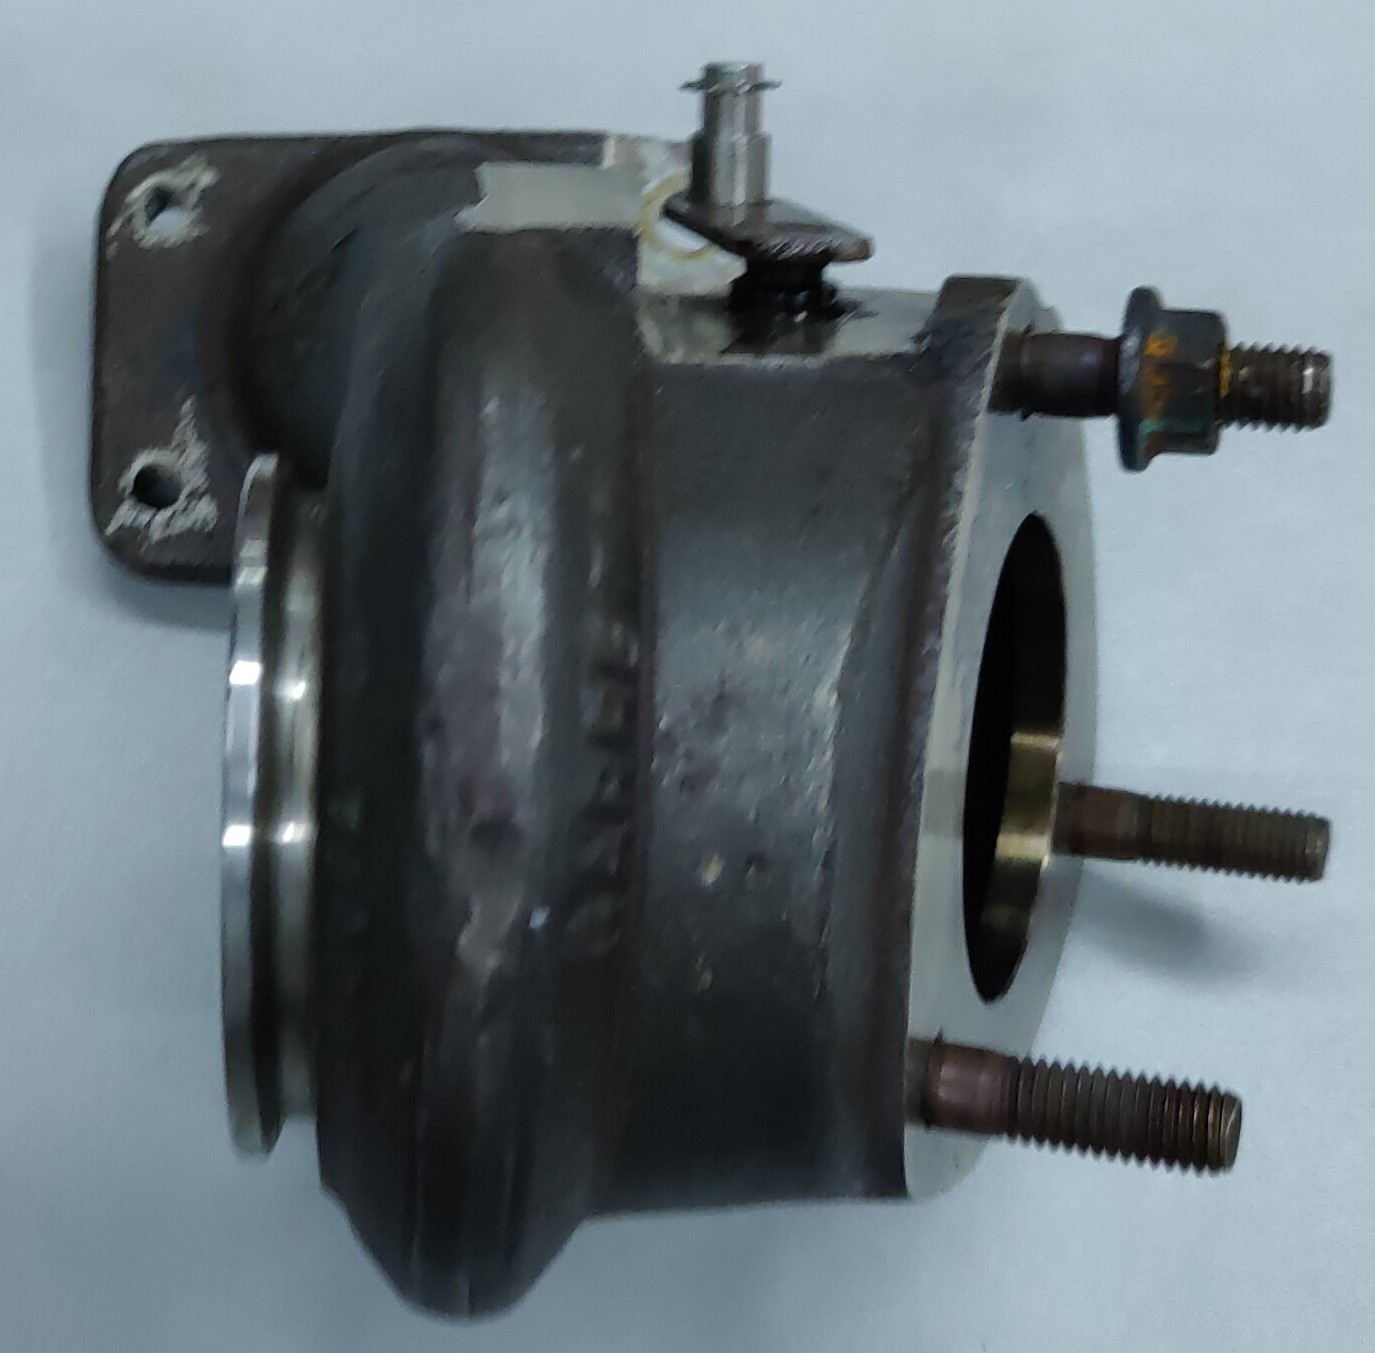
\includegraphics[width=\textwidth]{turbine}
		\caption{涡轮机}
		\label{turbine}
	\end{minipage}
	\begin{minipage}[b]{0.4\textwidth}
		\centering
		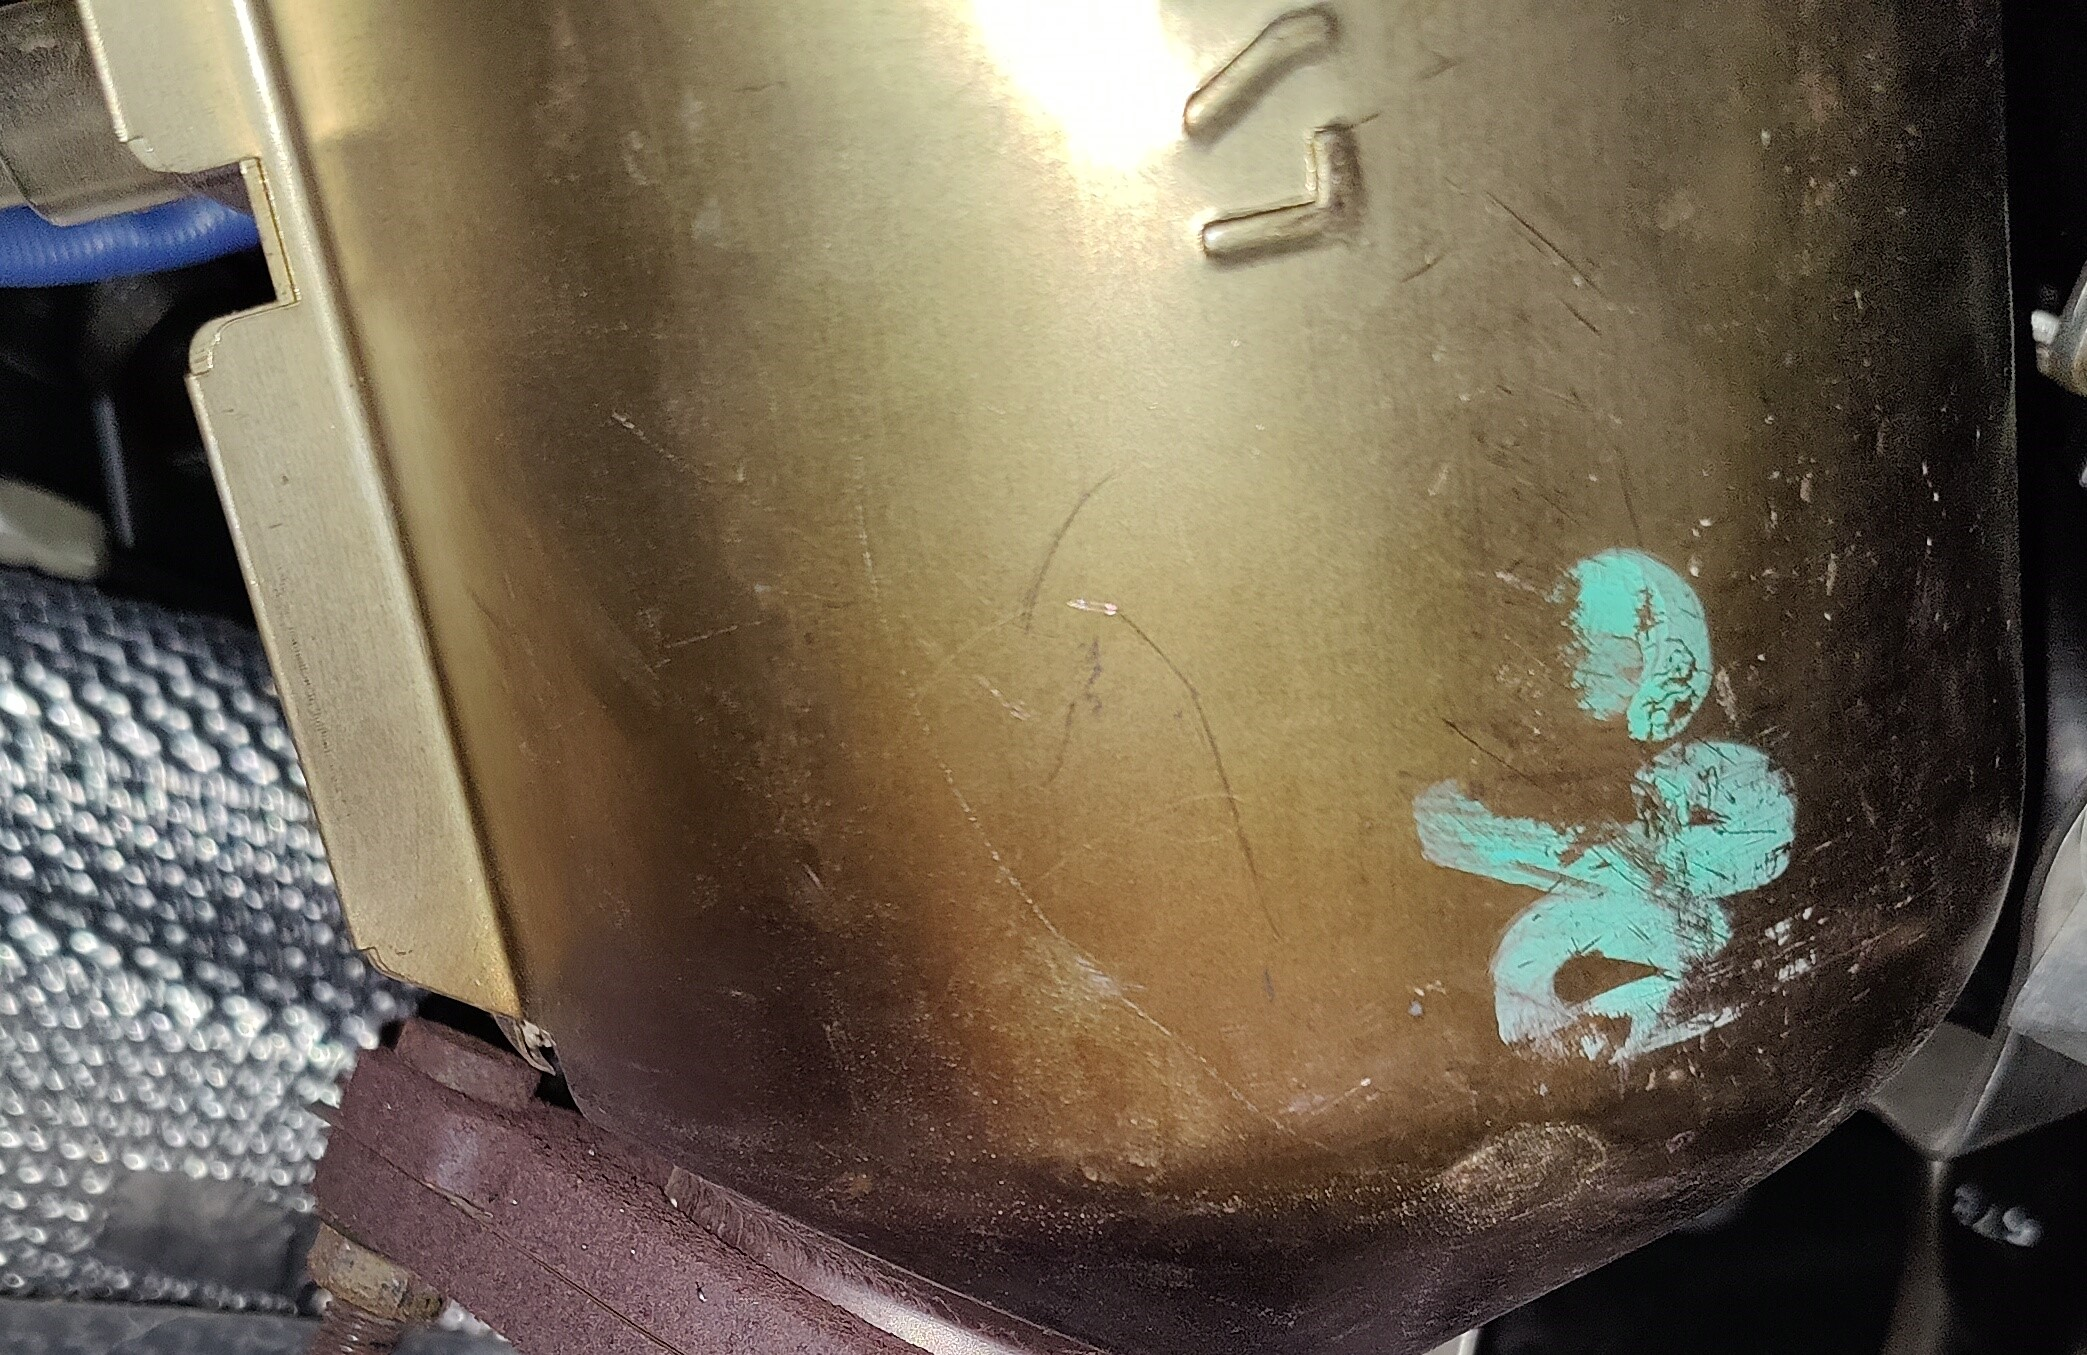
\includegraphics[width=\textwidth]{three-way catalytic converter}
		\caption{三元催化转换器}
		\label{three-way catalytic converter}
	\end{minipage}
	\begin{minipage}[b]{0.25\textwidth}
		\centering
		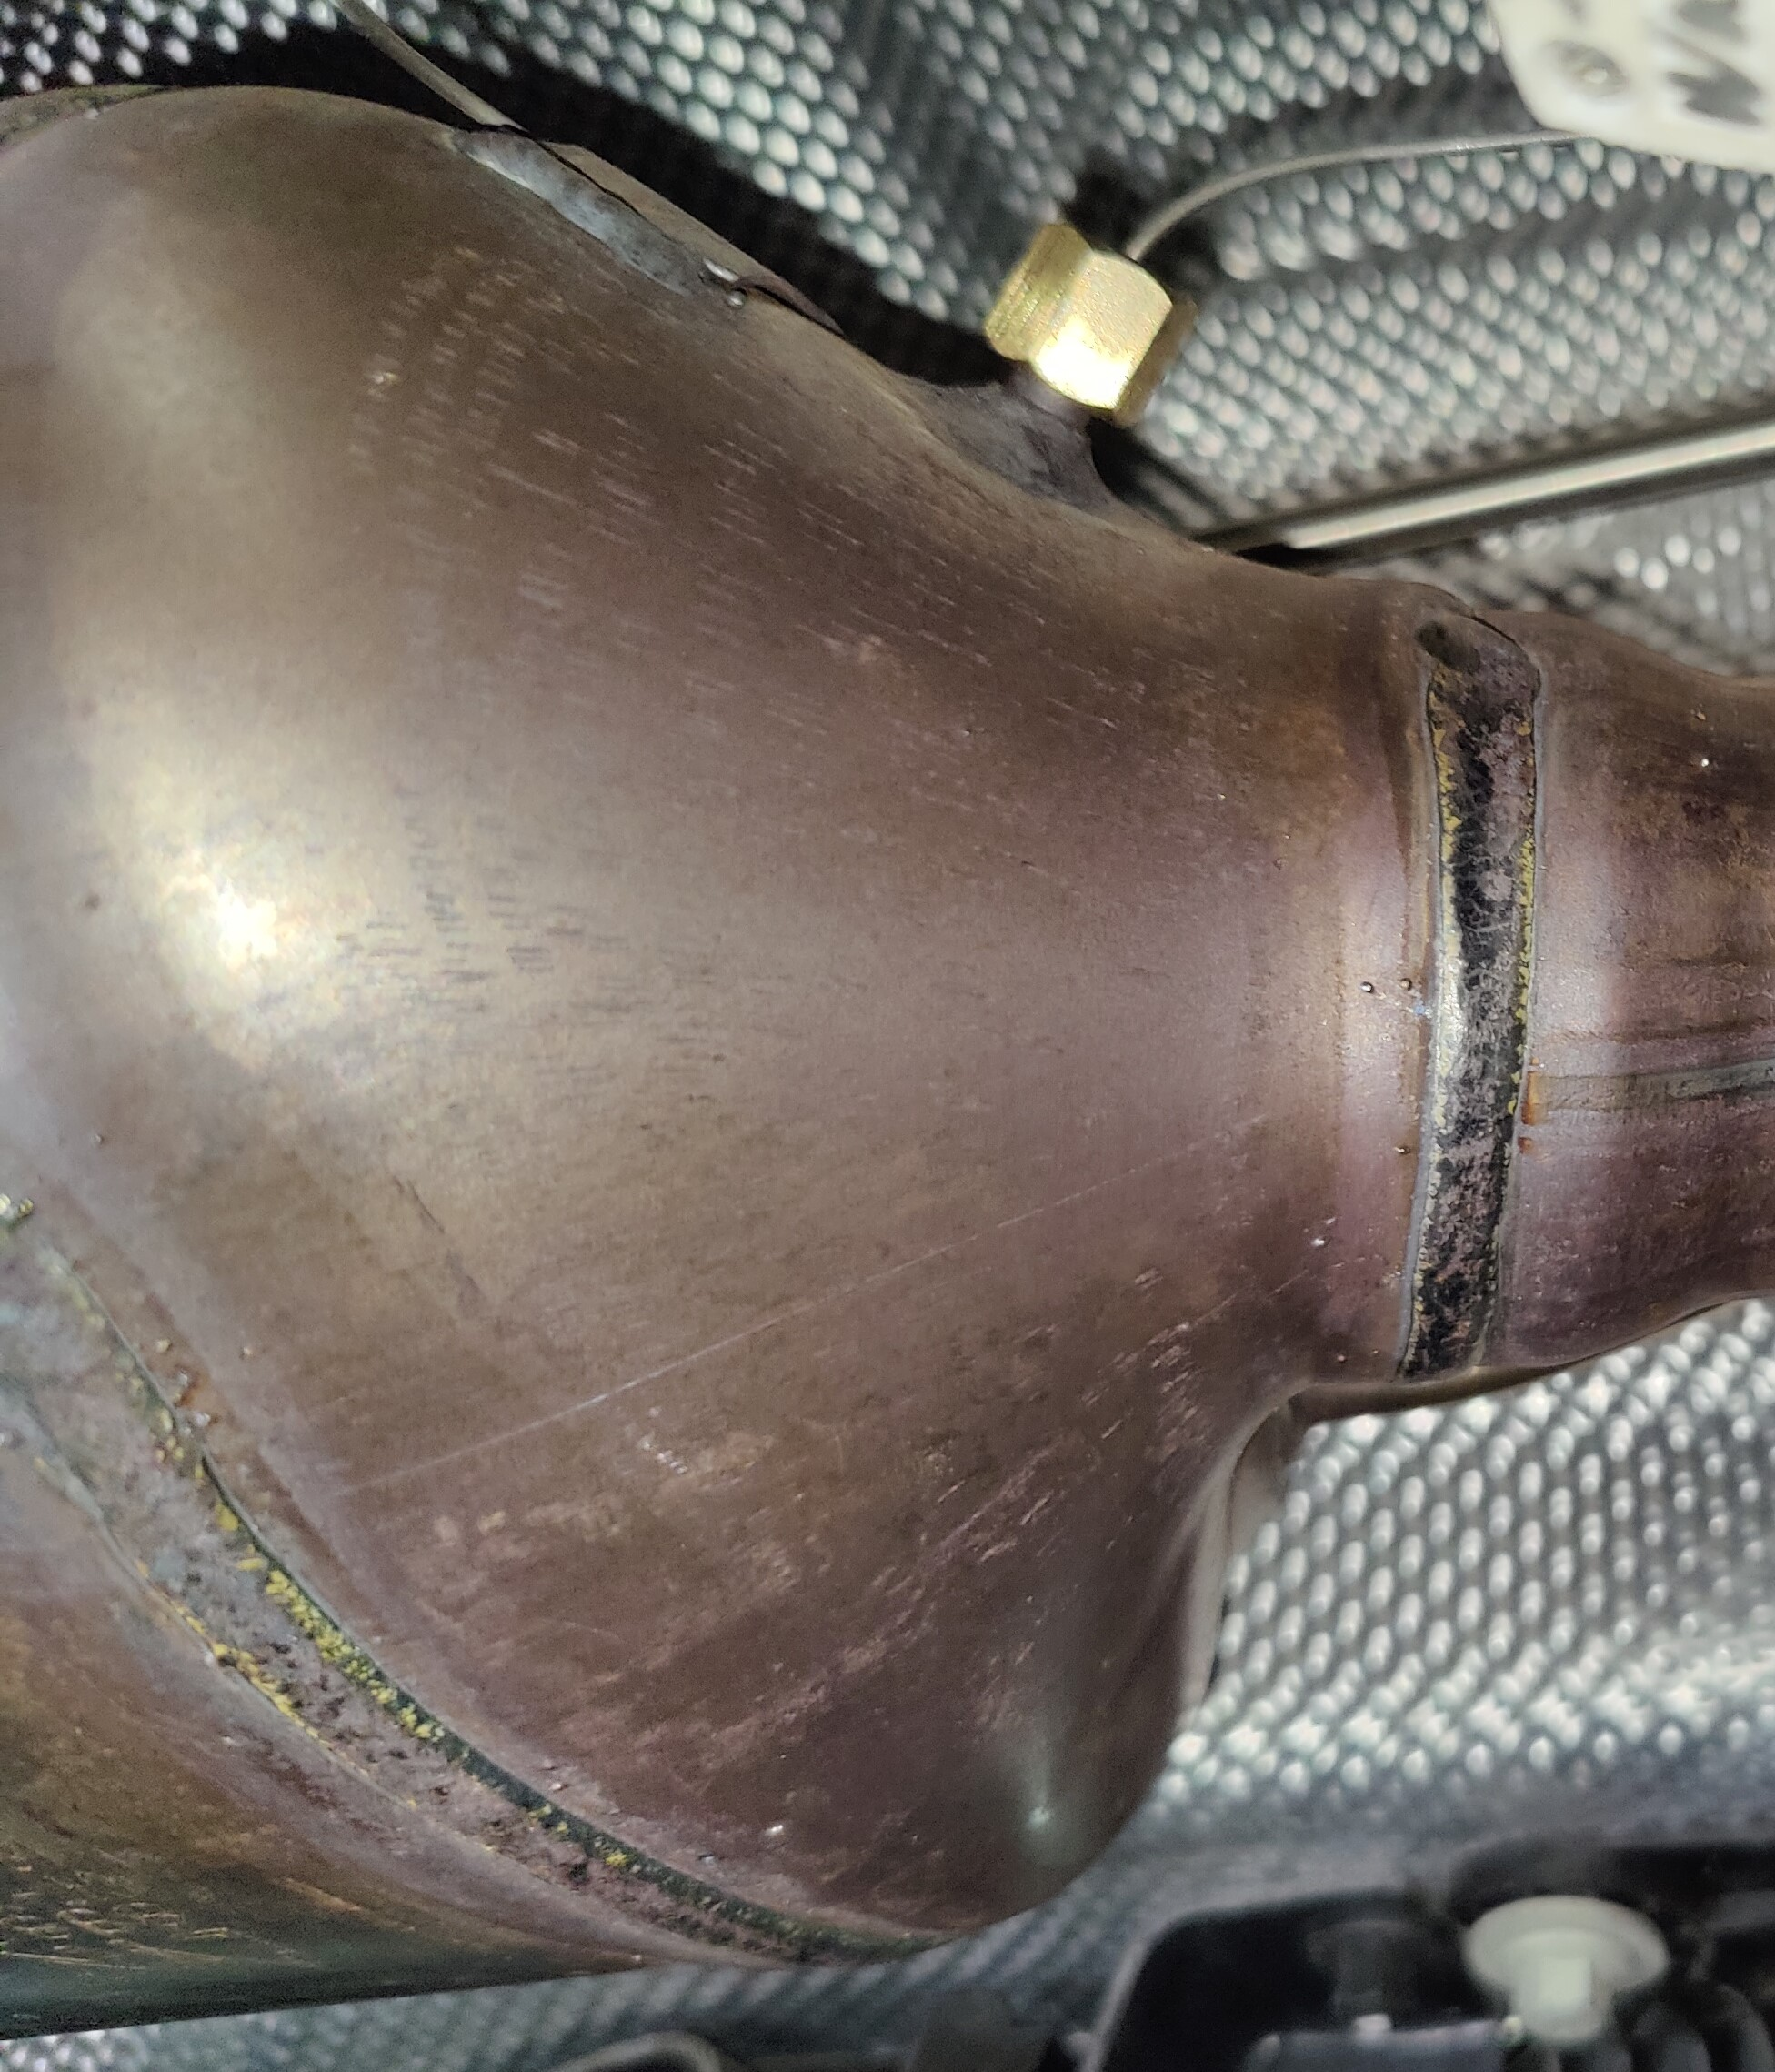
\includegraphics[width=\textwidth]{muffler F}
		\caption{前消声器}
		\label{muffler F}
	\end{minipage}
	\begin{minipage}[b]{0.55\textwidth}
		\centering
		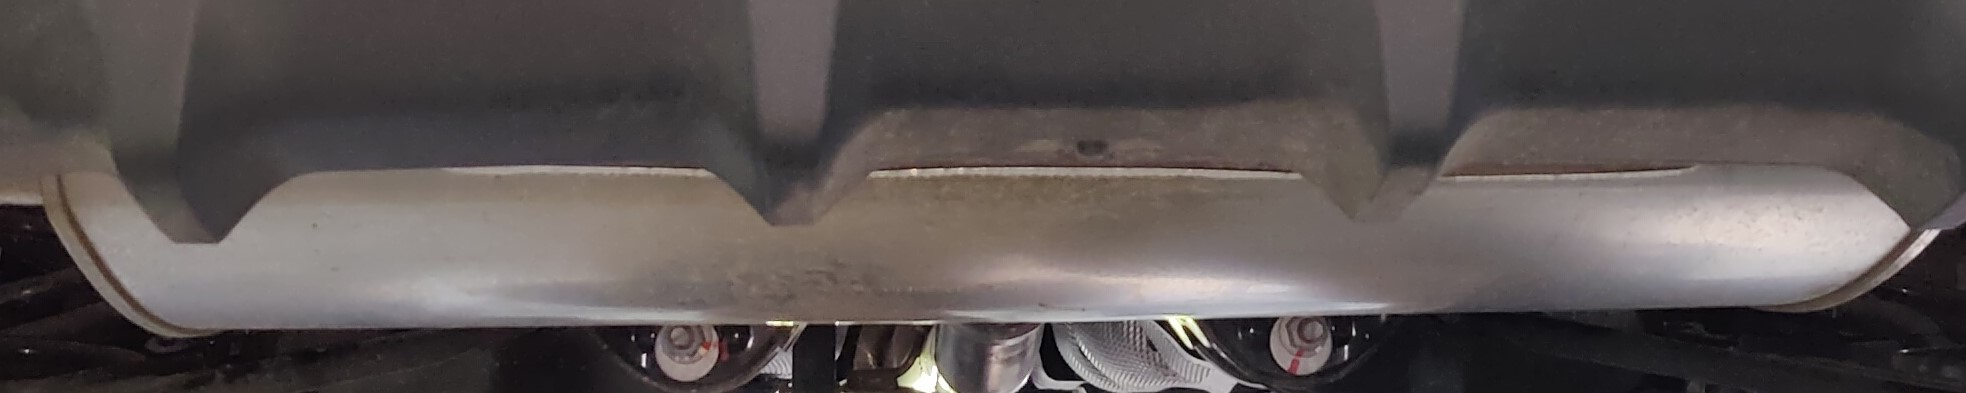
\includegraphics[width=\textwidth]{muffler B}
		\caption{后消声器}
		\label{muffler B}
	\end{minipage}
	\begin{minipage}[b]{0.4\textwidth}
		\centering
		\begin{minipage}[b]{0.45\textwidth}
			\centering
			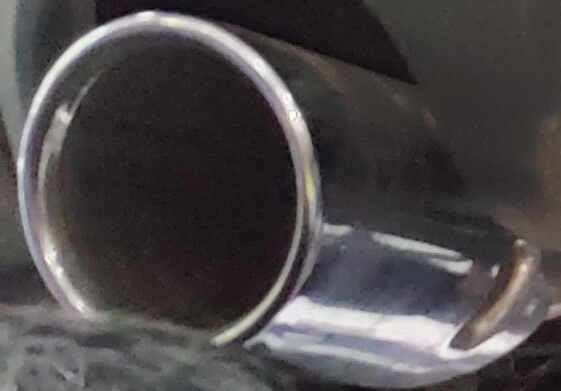
\includegraphics[width=\textwidth]{tail pipe L}
		\end{minipage}
		\begin{minipage}[b]{0.45\textwidth}
			\centering
			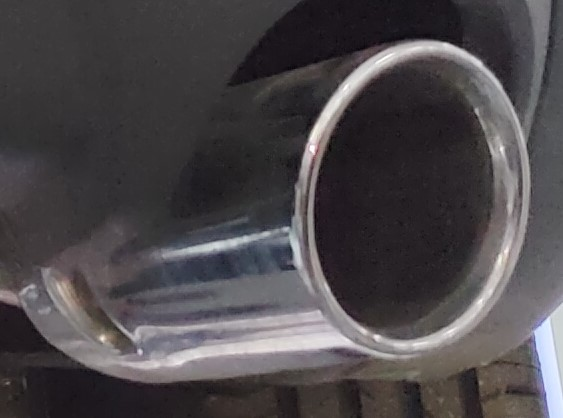
\includegraphics[width=\textwidth]{tail pipe R}
		\end{minipage}
		\caption{排气尾管}
		\label{tail pipe}
	\end{minipage}
\end{figure}

涡轮机是废气涡轮增压器(\cref{exhaust turbocharger})的一个重要组成部分,它的作用是把发动机排出废气的能量转化为机械功来驱动压气机叶轮。本车上使用的径流式涡轮,废气经进气蜗壳由叶轮的径向流入,经轴向流出。涡轮叶片一般在\SI{900}{\celsius}的高温排气冲击下工作,承受巨大的离心力,由镍基耐热合金钢或陶瓷材料制成;蜗壳用耐热合金铸铁铸成,外表面呈黑色,内表面光洁。

由于增压器的热负荷较大,单靠机油不足以满足增压器散热需求,\cref{exhaust turbocharger detached}中间那根较长的软管便是冷却水的管路,与发动机的冷却系统联通。冷却液自增压器中间体上的冷却液进口流入中间体水套,从冷却液出口流回发动机冷却系统。

\cref{exhaust turbocharger detached}所示的涡轮增压系统还带有放气阀(\cref{wastgate valve})。当增压压力达到一阈值后,ECU控制放气阀打开使部分排气不经过涡轮直接排出增压器,防止增压压力和涡轮转速过大造成压气机的阻塞。

\begin{figure}[htbp]
	\centering
	\begin{minipage}[b]{0.4\textwidth}
		\centering
		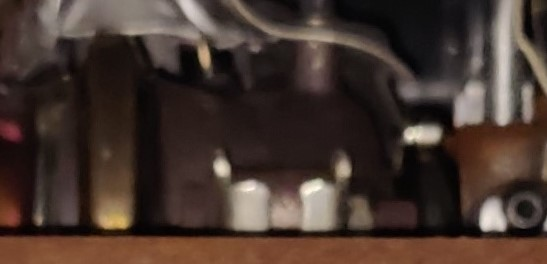
\includegraphics[width=\textwidth]{exhaust turbocharger}
		\caption{废气涡轮增压器}
		\label{exhaust turbocharger}
	\end{minipage}
	\centering
	\begin{minipage}[b]{0.35\textwidth}
		\centering
		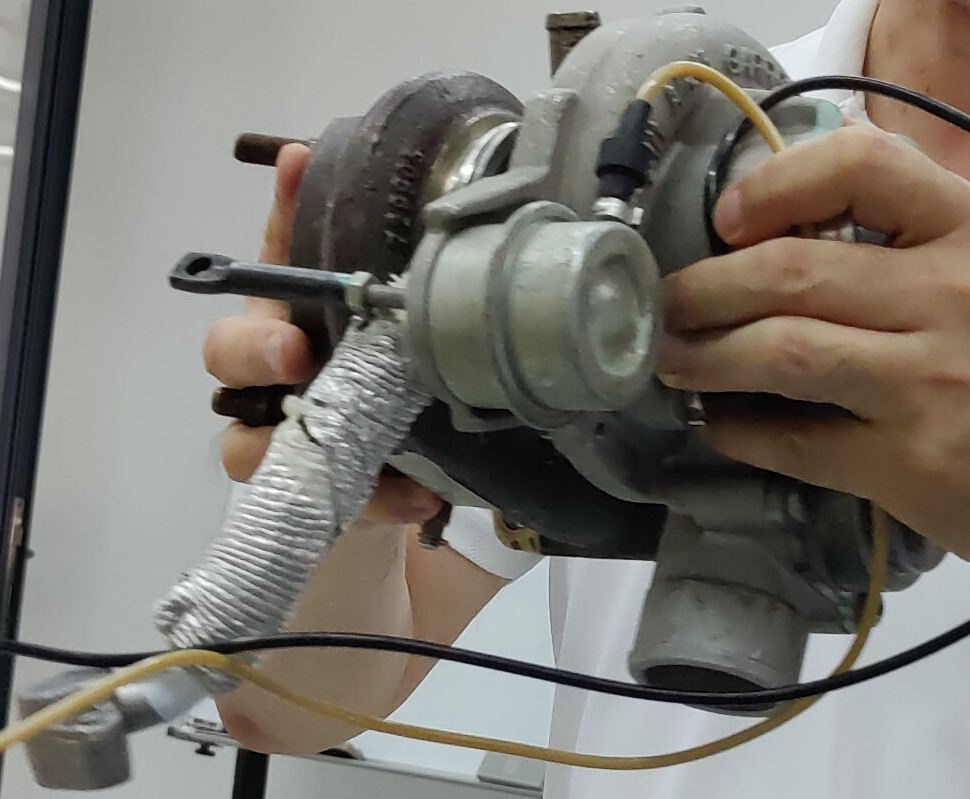
\includegraphics[width=0.8\textwidth]{exhaust turbocharger detached}
		\caption{拆下的废气涡轮增压器}
		\label{exhaust turbocharger detached}
	\end{minipage}
	\begin{minipage}[b]{0.18\textwidth}
		\centering
		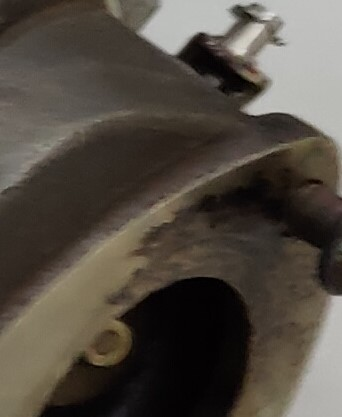
\includegraphics[width=\textwidth]{wastgate valve}
		\caption{放气阀}
		\label{wastgate valve}
	\end{minipage}
\end{figure}

三元催化转换器以排气中的\ce{CO}和\ce{HC}作为还原剂,在把\ce{NO_x}还原成\ce{N2}和\ce{O2}的同时把\ce{CO}和\ce{HC}氧化为\ce{CO2}和\ce{H2O},反应式为
\begin{align}
	\ce{CO + O2 & -> CO2} \nonumber       \\
	\ce{HC + O2 & -> H2O + CO2} \nonumber \\
	\ce{NO_X    & -> N2 + O2} \nonumber
\end{align}
三元催化转换器将带有很多小孔的蜂窝状陶瓷作为载体,表面附着一层薄的氧化铝中间镀层,再在其上镀以由铂、钯、铑等贵金属制成的催化剂。催化转换器外面用金属外壳封闭,并焊在排气管路内,避免被随意拆卸。三元催化转换器要求车辆使用无铅汽油,温度超过\SI{350}{\celsius}时才会工作,最重要的是要求发动机混合气浓度始终在理论空燃比附近。最后这点是通过氧传感器实现的。

三元催化转换器前后各有一个氧传感器,其中前氧传感器起主要作用,后氧传感器的用处主要是检测催化转换器是否工作正常。ECU通过进气量、喷油量及排气中氧浓度可实现过量空气系数$\lambda$的闭环控制。氧传感器的传感元件一般是在陶瓷管基体上附着有\ce{ZrO2}涂层,外侧通排气,内侧通大气。当陶瓷管温度在\SI{350}{\celsius}左右时具有固态电解质的特性。如\cref{voltage response curve},当混合气偏浓时,排气中\ce{O2}浓度低,陶瓷管内外\ce{O^2-}浓度差较高,氧传感器输出电压高(约\SI{900}{\mV});反之当混合气偏稀时输出电压较低(约\SI{100}{\mV})。氧传感器输出电压在理论空燃比附近对过量空气系数的变化很敏感,ECU据此不断修正喷油量使得$\lambda$始终在最佳范围内。

由于缸内直喷易产生碳烟,排气系统上设置有颗粒捕集器以满足排放法规要求。

\begin{figure}[htbp]
	\centering
	\begin{minipage}[b]{0.45\textwidth}
		\centering
		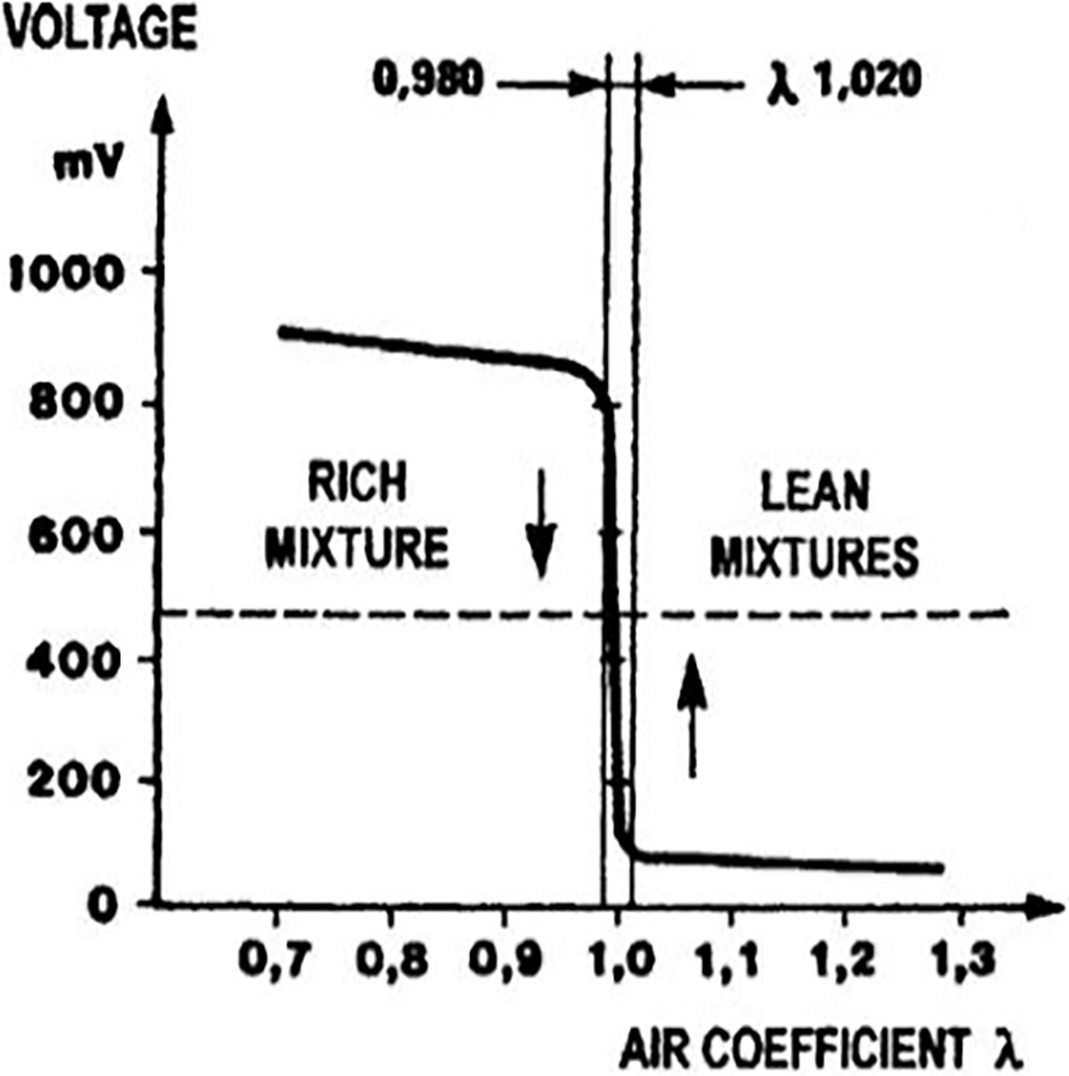
\includegraphics[width=\textwidth]{voltage response curve}
		\caption{氧传感器的电压曲线}
		\label{voltage response curve}
	\end{minipage}
\end{figure}

消声器的主要功能是减小排气的噪声。由于发动机为间歇排气,在排气管中会引起压力的脉动,排气的温度、压力、速度等也很高,具有一定能量。消声器的通过吸收、扩张、共振、干涉等方式耗散排气中的能量,达到消声的目的。一个消声器中常有不同形式的多个腔组合(\cref{muffler dissect}),以提高消声效果。

\begin{figure}[htbp]
	\centering
	\begin{minipage}[b]{0.6\textwidth}
		\centering
		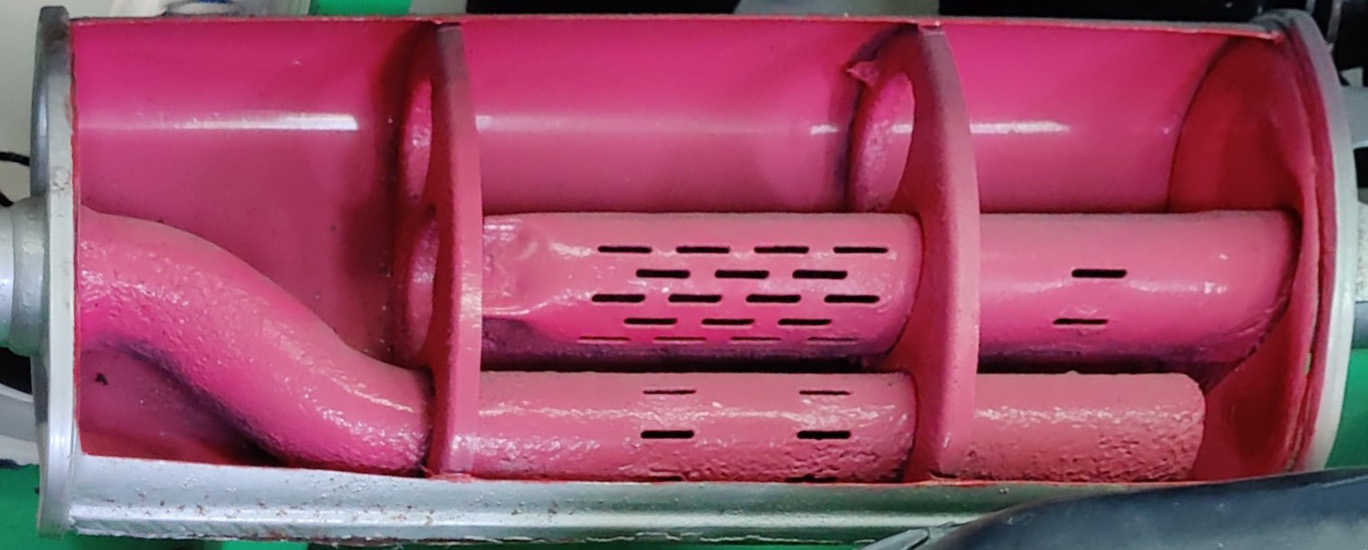
\includegraphics[width=\textwidth]{muffler dissect}
		\caption{剖开的排气消声器}
		\label{muffler dissect}
	\end{minipage}
\end{figure}

\subsection{请简述汽车动力总成如何固定在车身上。}

发动机和变速箱刚性连接构成汽车动力总成,但动力总成与车身的连接是柔性的,这需要通过悬置来实现。悬置的功用主要有支撑、限位和隔振。支撑指悬置必须能承受动力总成的质量,使其不至于产生过大的静位移;限位指动力总成在受到各种干扰力作用的情况下,悬置应能有效的限制其最大位移以避免干涉;隔振指悬置一方面要阻止作为振源的发动机向车身传递振动,另一方面还要能缓和路面不平激励等传给发动机的振动和冲击。

从隔振角度来说,希望悬置较软,以期将振动更好地隔离;而从支承和限位角度来说,为使发动机舱能布置紧凑,又希望悬置越硬越好。在悬置设计中如何最优化选取悬置刚度是一个极为重要的问题。同时,为了使振动得到迅速衰减,发动机悬置还应具有适当的的阻尼。

领克02车型的动力总成采用三点固定的方式,通过一个后悬置和两个前悬置将动力总成与车身连接,如\cref{mount}。\cref{mount B}看得较清楚,我们可以看到,后悬置与发动机和车身的两个连接轴线互相垂直,且两连接处都有橡胶减振块,能有效衰减动力总成相对车身俯仰和偏航两个方向的相对运动,而对侧倾的衰减主要由前面两悬置实现。

当然,这种软连接的形式会对发动机的动力输出造成一定影响,因为部分扭矩被用于克服减振块的阻力。在一些超跑和方程式赛车中有将发动机直接固定在单体壳上的方式,以期最大化动力输出,但会恶化车辆的NVH (Noise, vibration, and harshness) 特性,在乘用车上一般都是用三点式或四点式的悬置将汽车动力总成固定在车身上。

\begin{figure}[htbp]
	\centering
	\subfigure[后悬置]{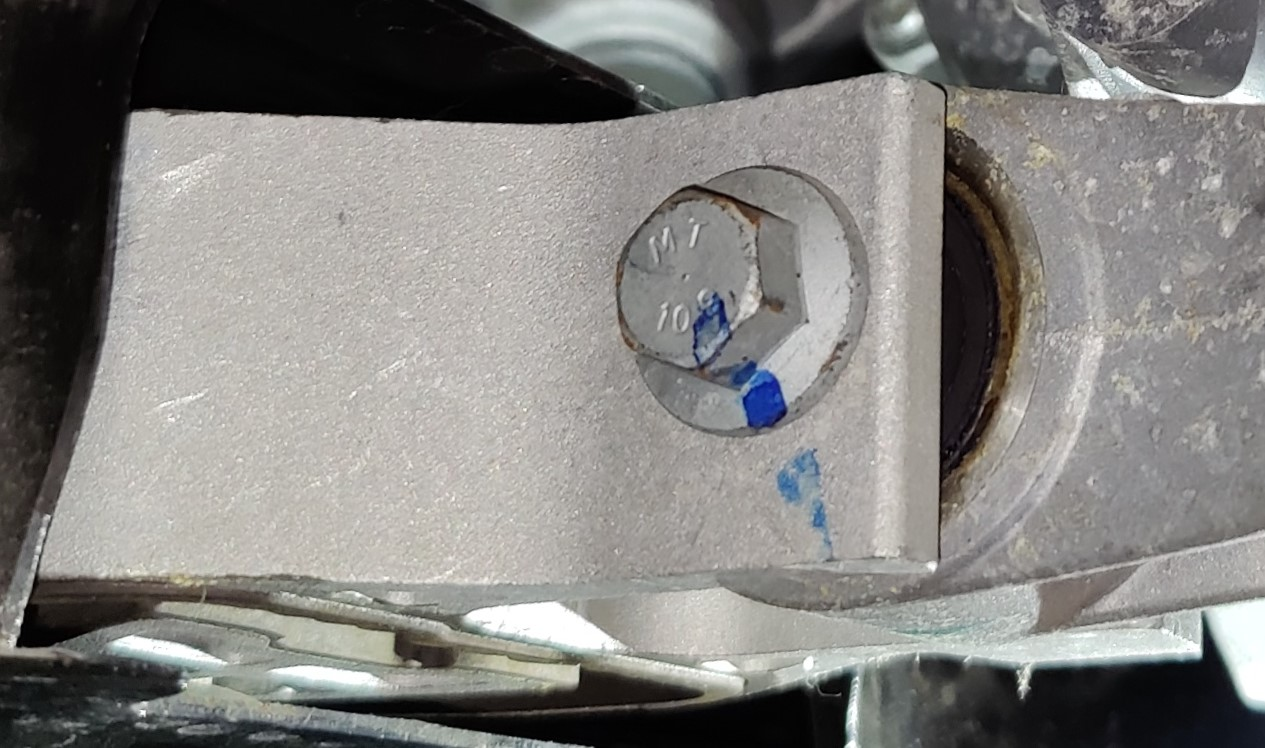
\includegraphics[width=0.6\textwidth]{mount B}\label{mount B}}
	\subfigure[右前悬置]{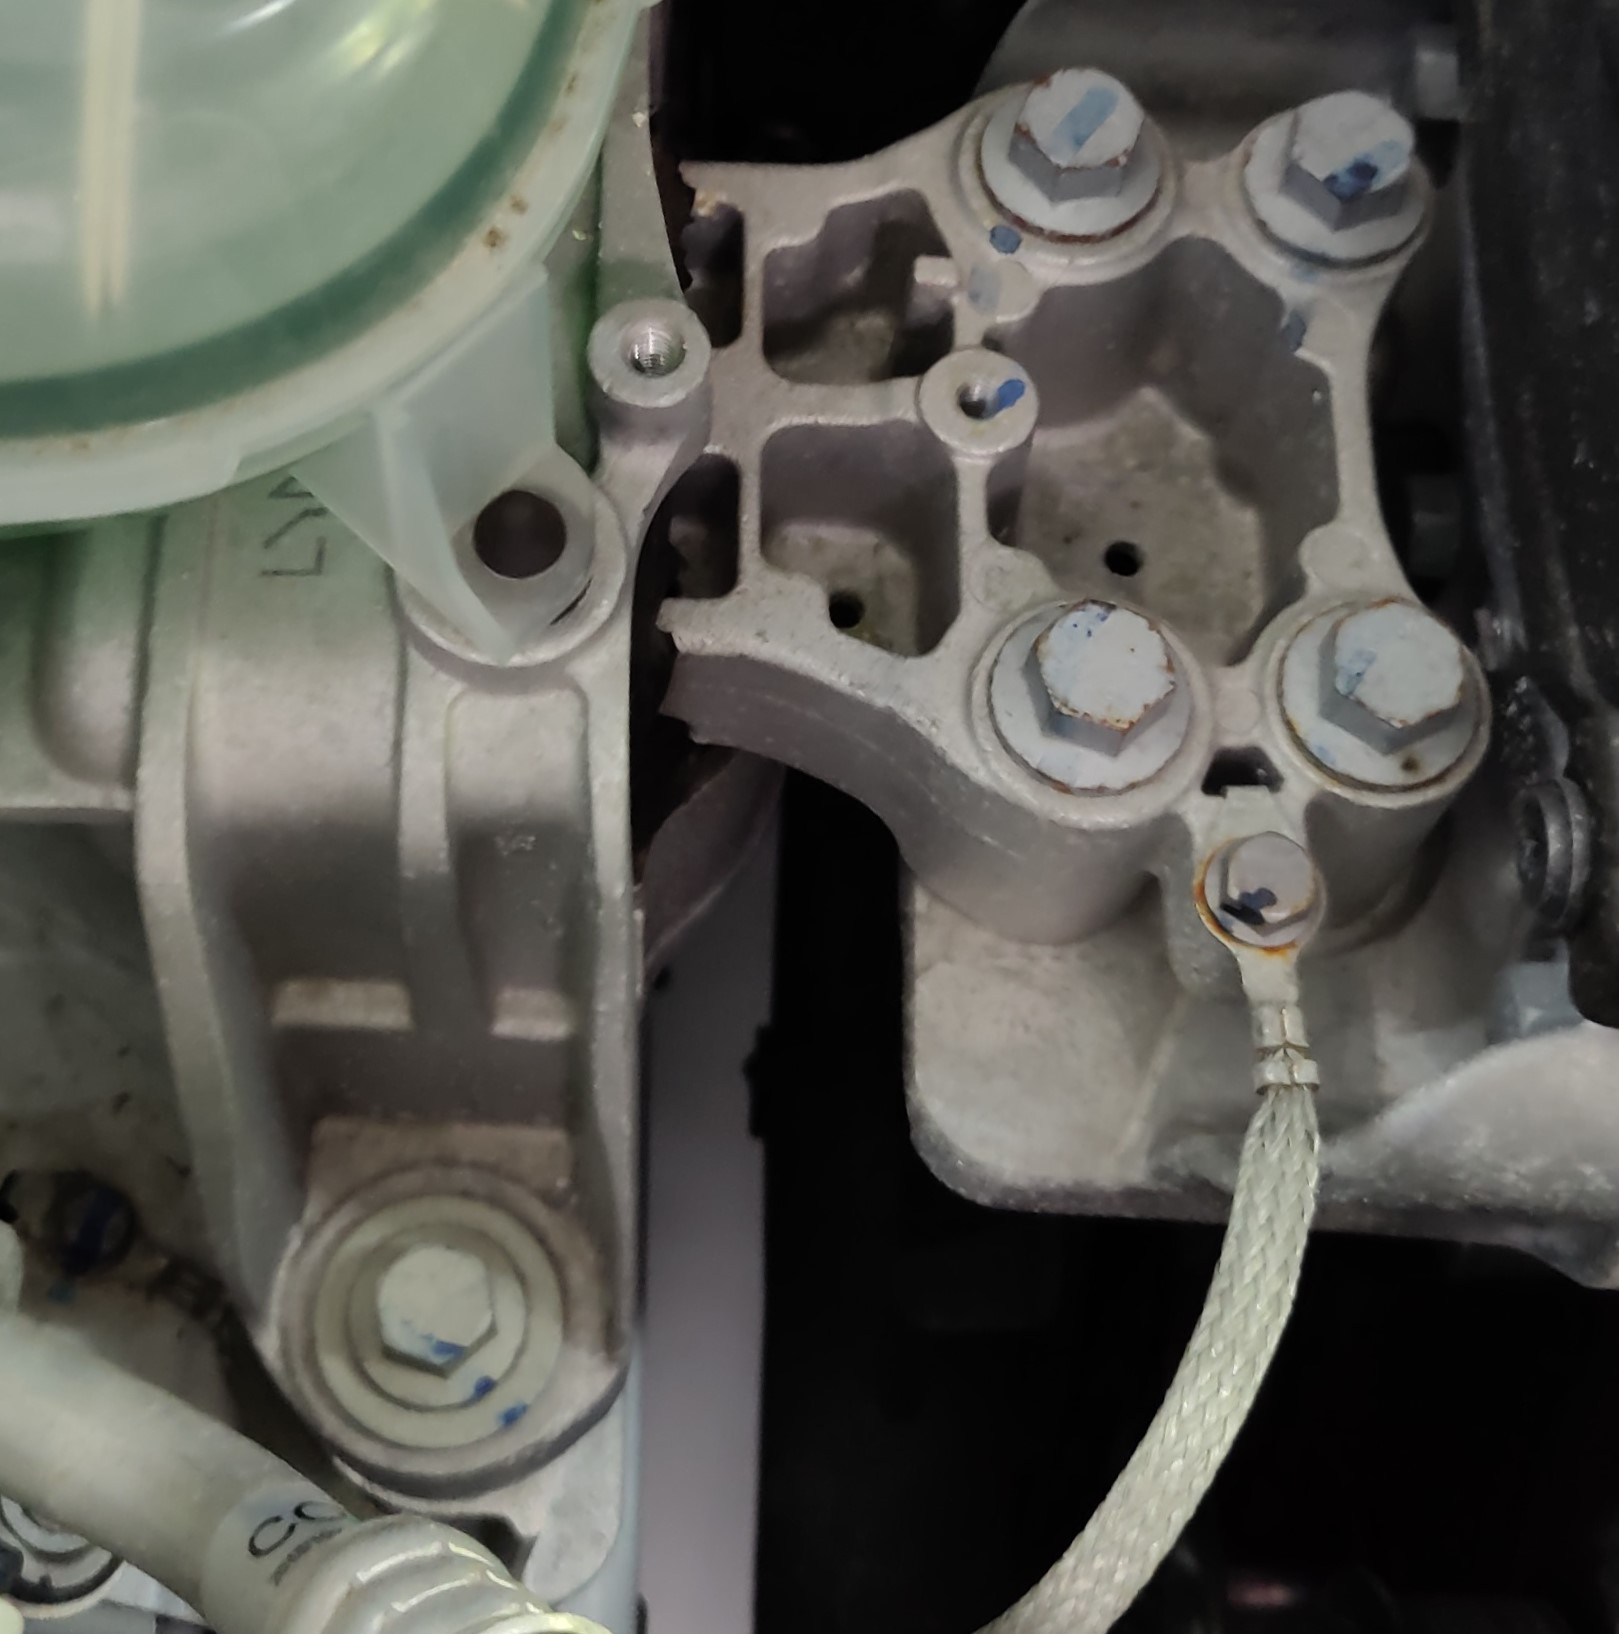
\includegraphics[width=0.4\textwidth]{mount RF}\label{mount RF}}
	\subfigure[左前悬置]{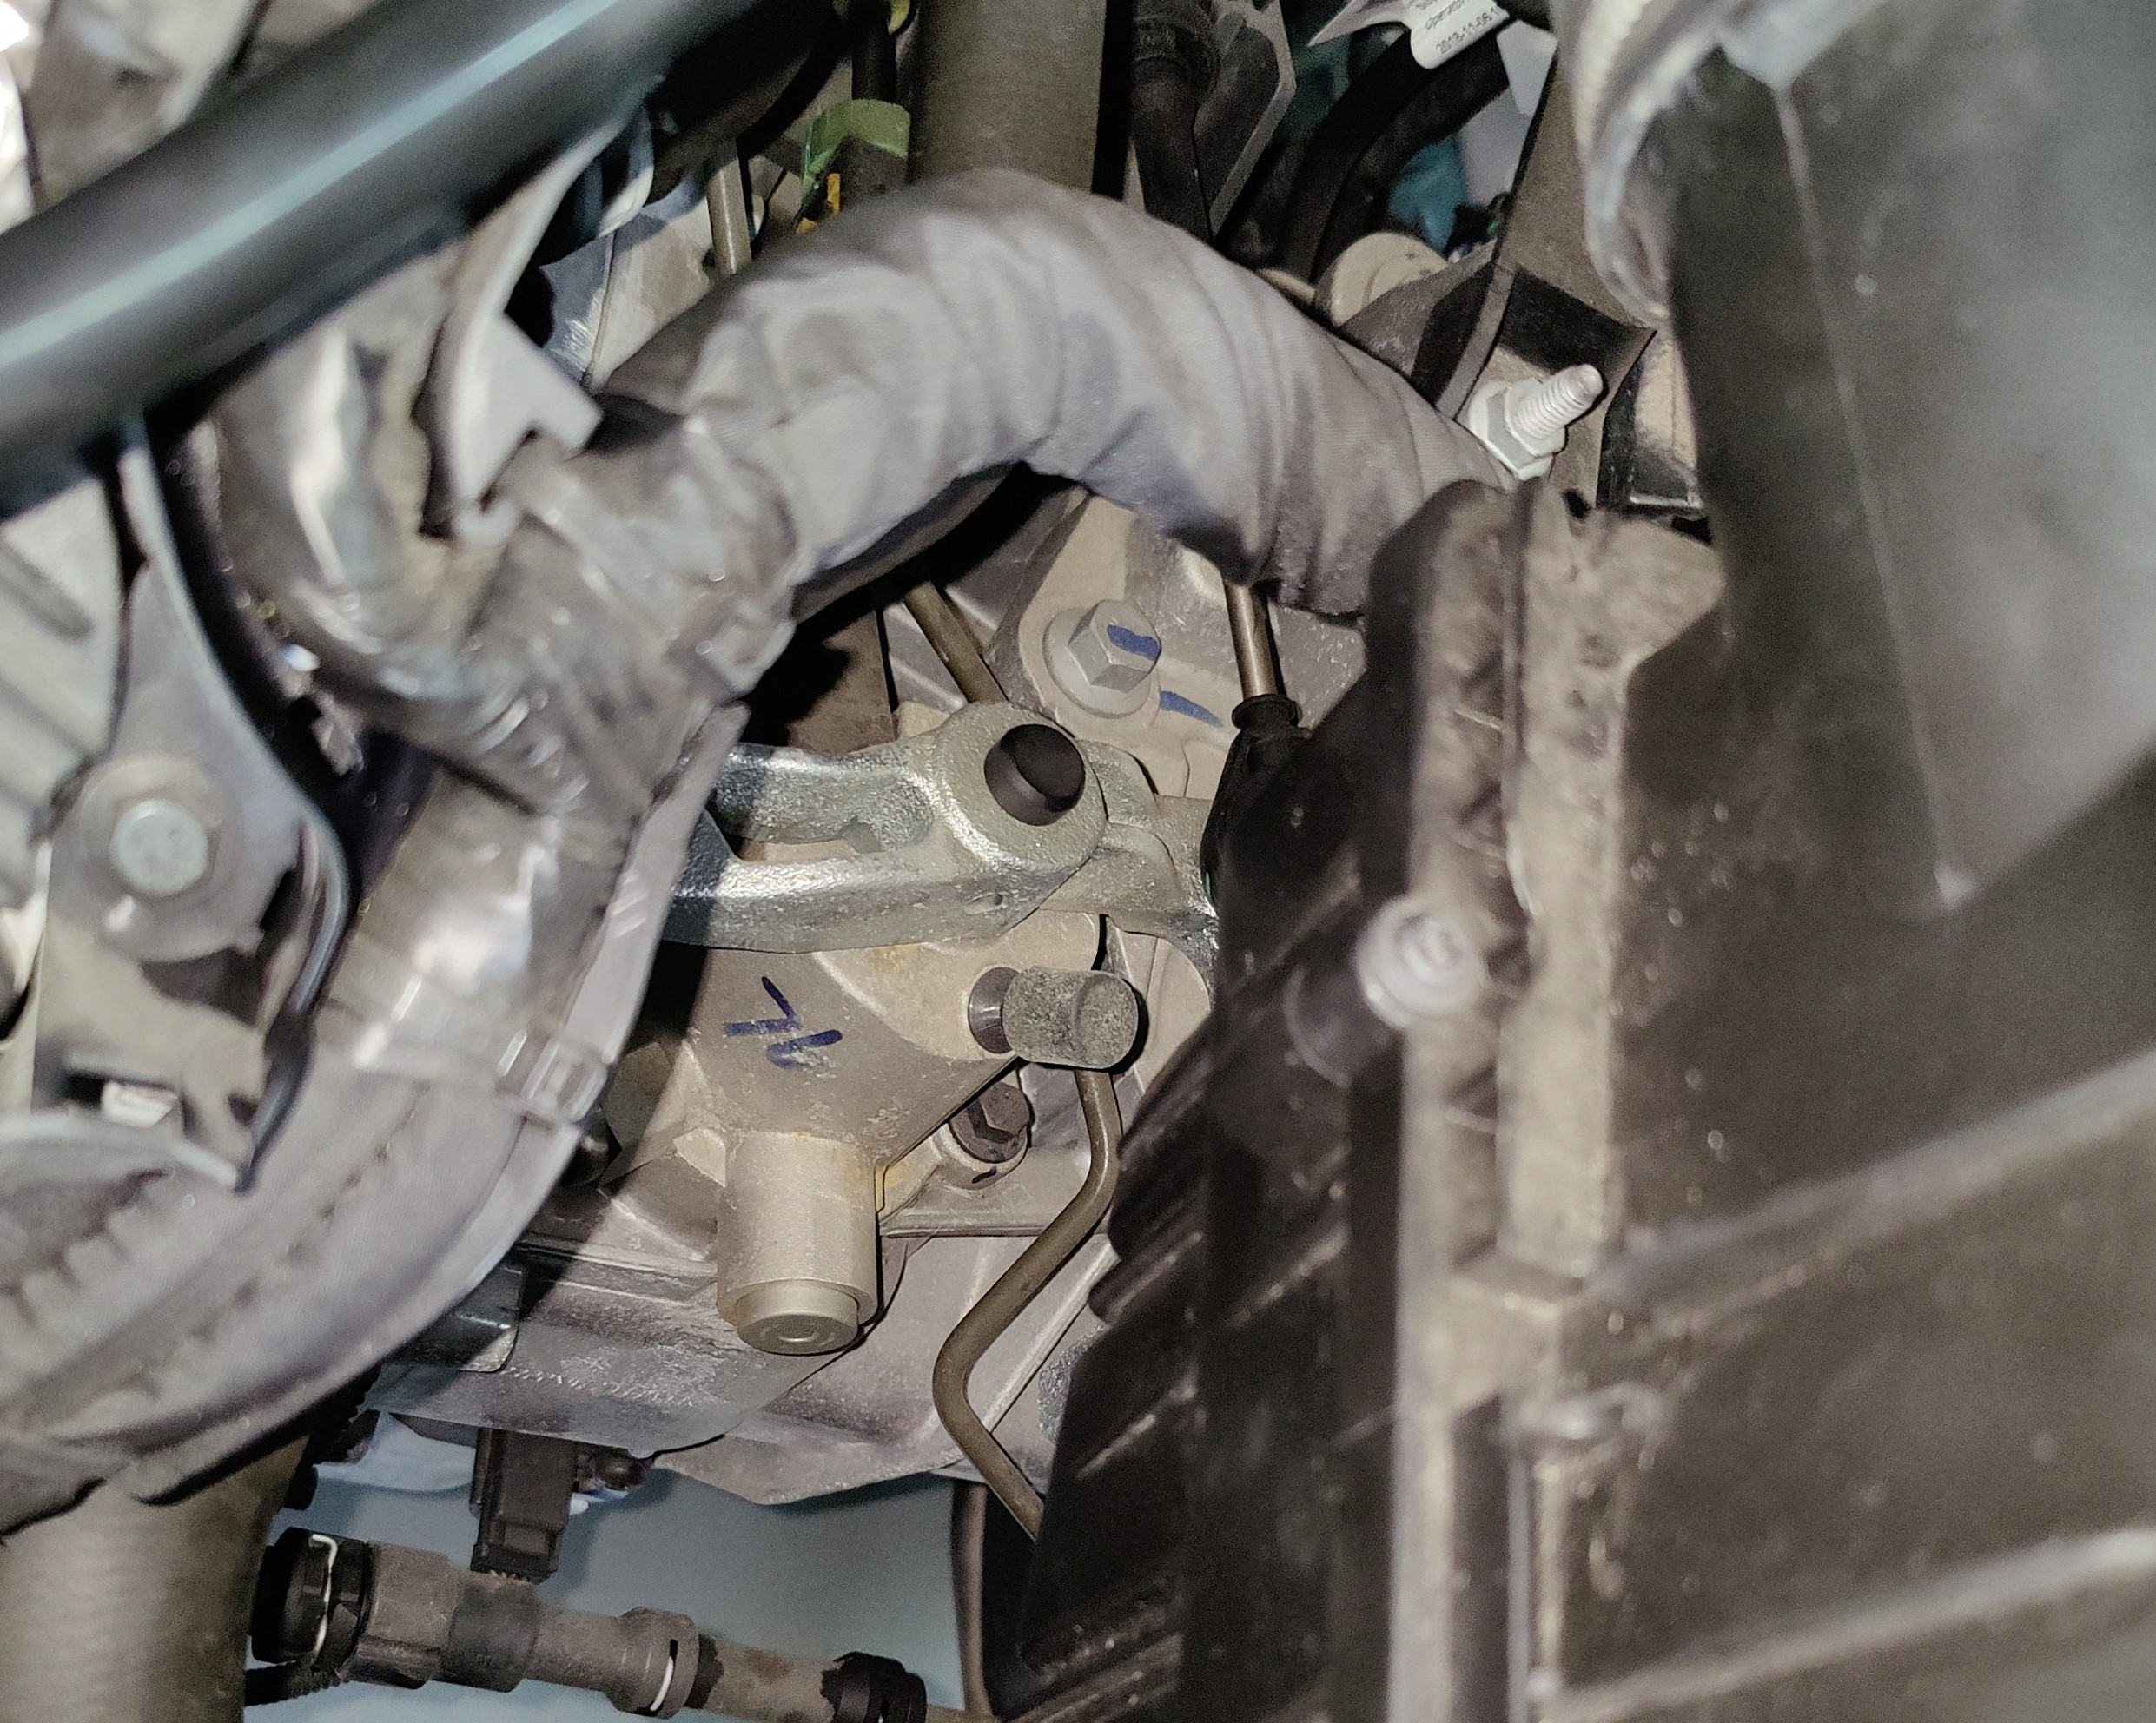
\includegraphics[width=0.5\textwidth]{mount LF}\label{mount LF}}
	\caption{悬置}
	\label{mount}
\end{figure}

\subsection{请简述发动机的控制系统中的传感器和执行器主要有哪些?}

发动机控制系统中的传感器主要有空气流量计、曲轴位置传感器、氧传感器、节气门位置传感器、冷却液温度传感器、爆震传感器、离合器开关;执行器主要有燃油泵继电器、燃油泵、喷油器、点火线圈、凸轮轴调节阀、节气门电机(\cref{sensors and actuators})。

\begin{figure}[htbp]
	\centering
	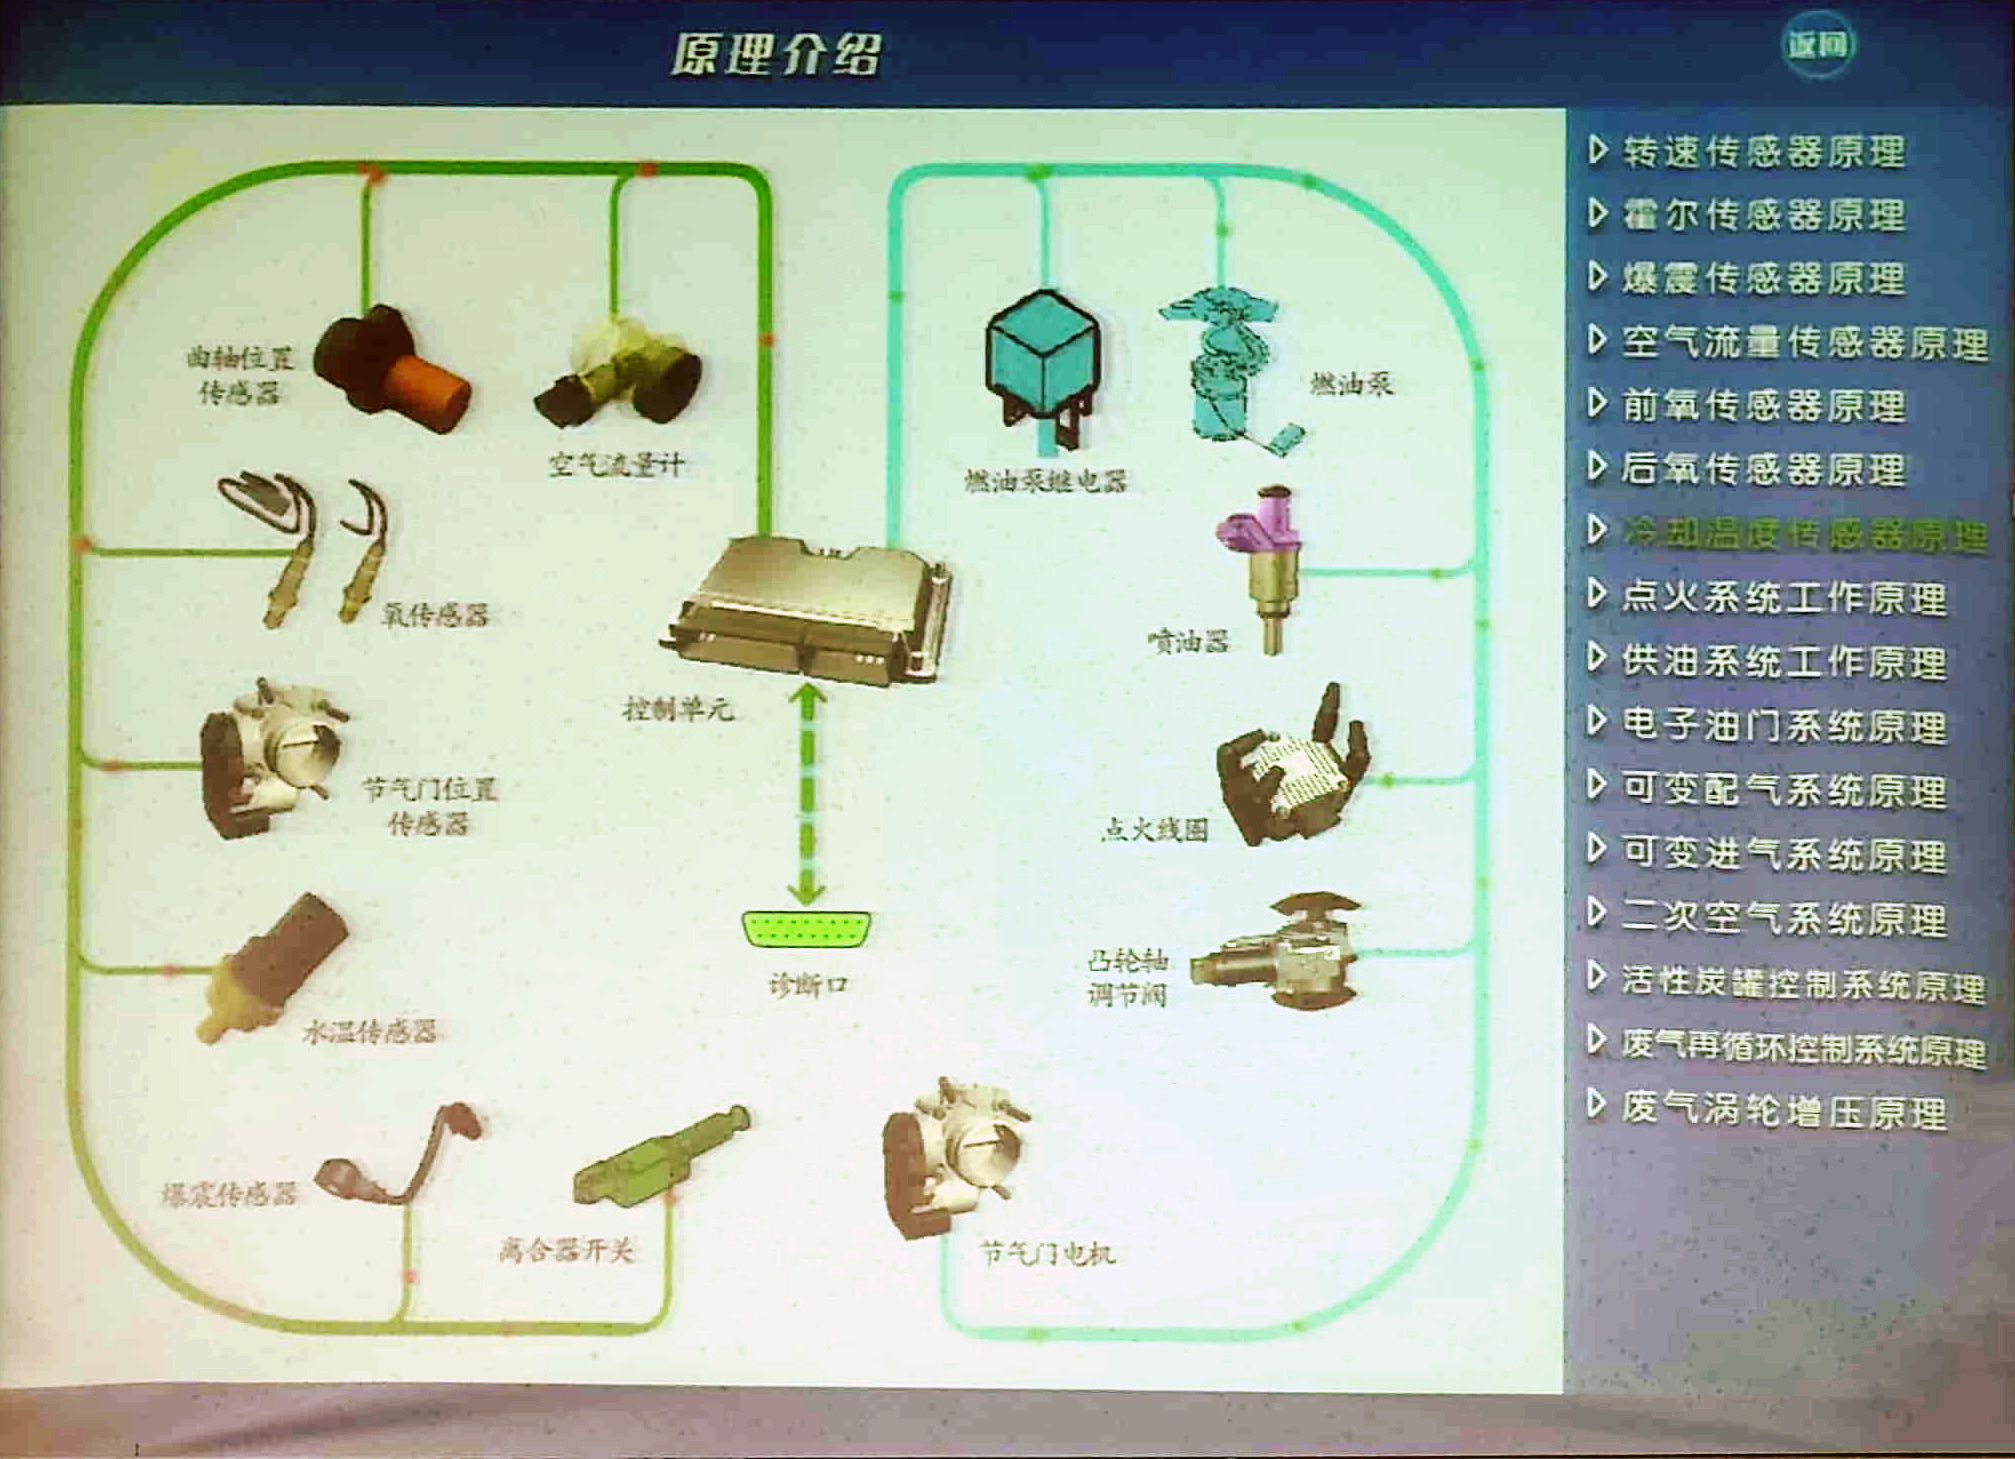
\includegraphics[width=0.9\textwidth]{sensors and actuators}
	\caption{发动机的控制系统中的传感器和执行器}
	\label{sensors and actuators}
\end{figure}

\cref{sensors}所示为发动机控制系统中的部分传感器。现在车用的空气流量计多能直接测得空气的质量流量,分为热线式和热膜式两种,ECU根据空气供给的多少确定喷油量,保证空燃比在理论空燃比附近。曲轴位置传感器有磁电式、光电式和霍尔式等,与安装在曲轴上的靶轮共同工作,主要用于用检测发动机转速,并在凸轮轴相位传感器的配合下确定各缸压缩上止点。前氧传感器和后氧传感器结构类似,都能将排气中氧浓度和空气氧浓度的差转化为输出电压供ECU实现$\lambda$闭环控制。节气门位置传感器是电子节气门系统的一部分,让ECU能闭环控制节气门位置。冷却液温度传感器装在发动机冷却液的出水口上,用来检测出水温度,这个温度一般控制在\SI{90}{\celsius}左右,过高或过低对发动机的工作都是不利的。冷却液温度可通过节温器进行反馈调节,当温度较低时只让冷却液在小回路中循环,便于发动机快速升温;温度高时开启大回路,给发动机较快降温。爆震传感器安装在发动机机体上,它的固有频率设计为与爆震发生时机体的震动频率相近。当发生爆震时,发动机机体与传感器发生共振,传感器输出最大电压信号,表示爆震发生,ECU据此推迟点火,即减小点火提前角,这能有效抑制发动机爆燃。

\begin{figure}[htbp]
	\centering
	\subfigure[空气流量计]{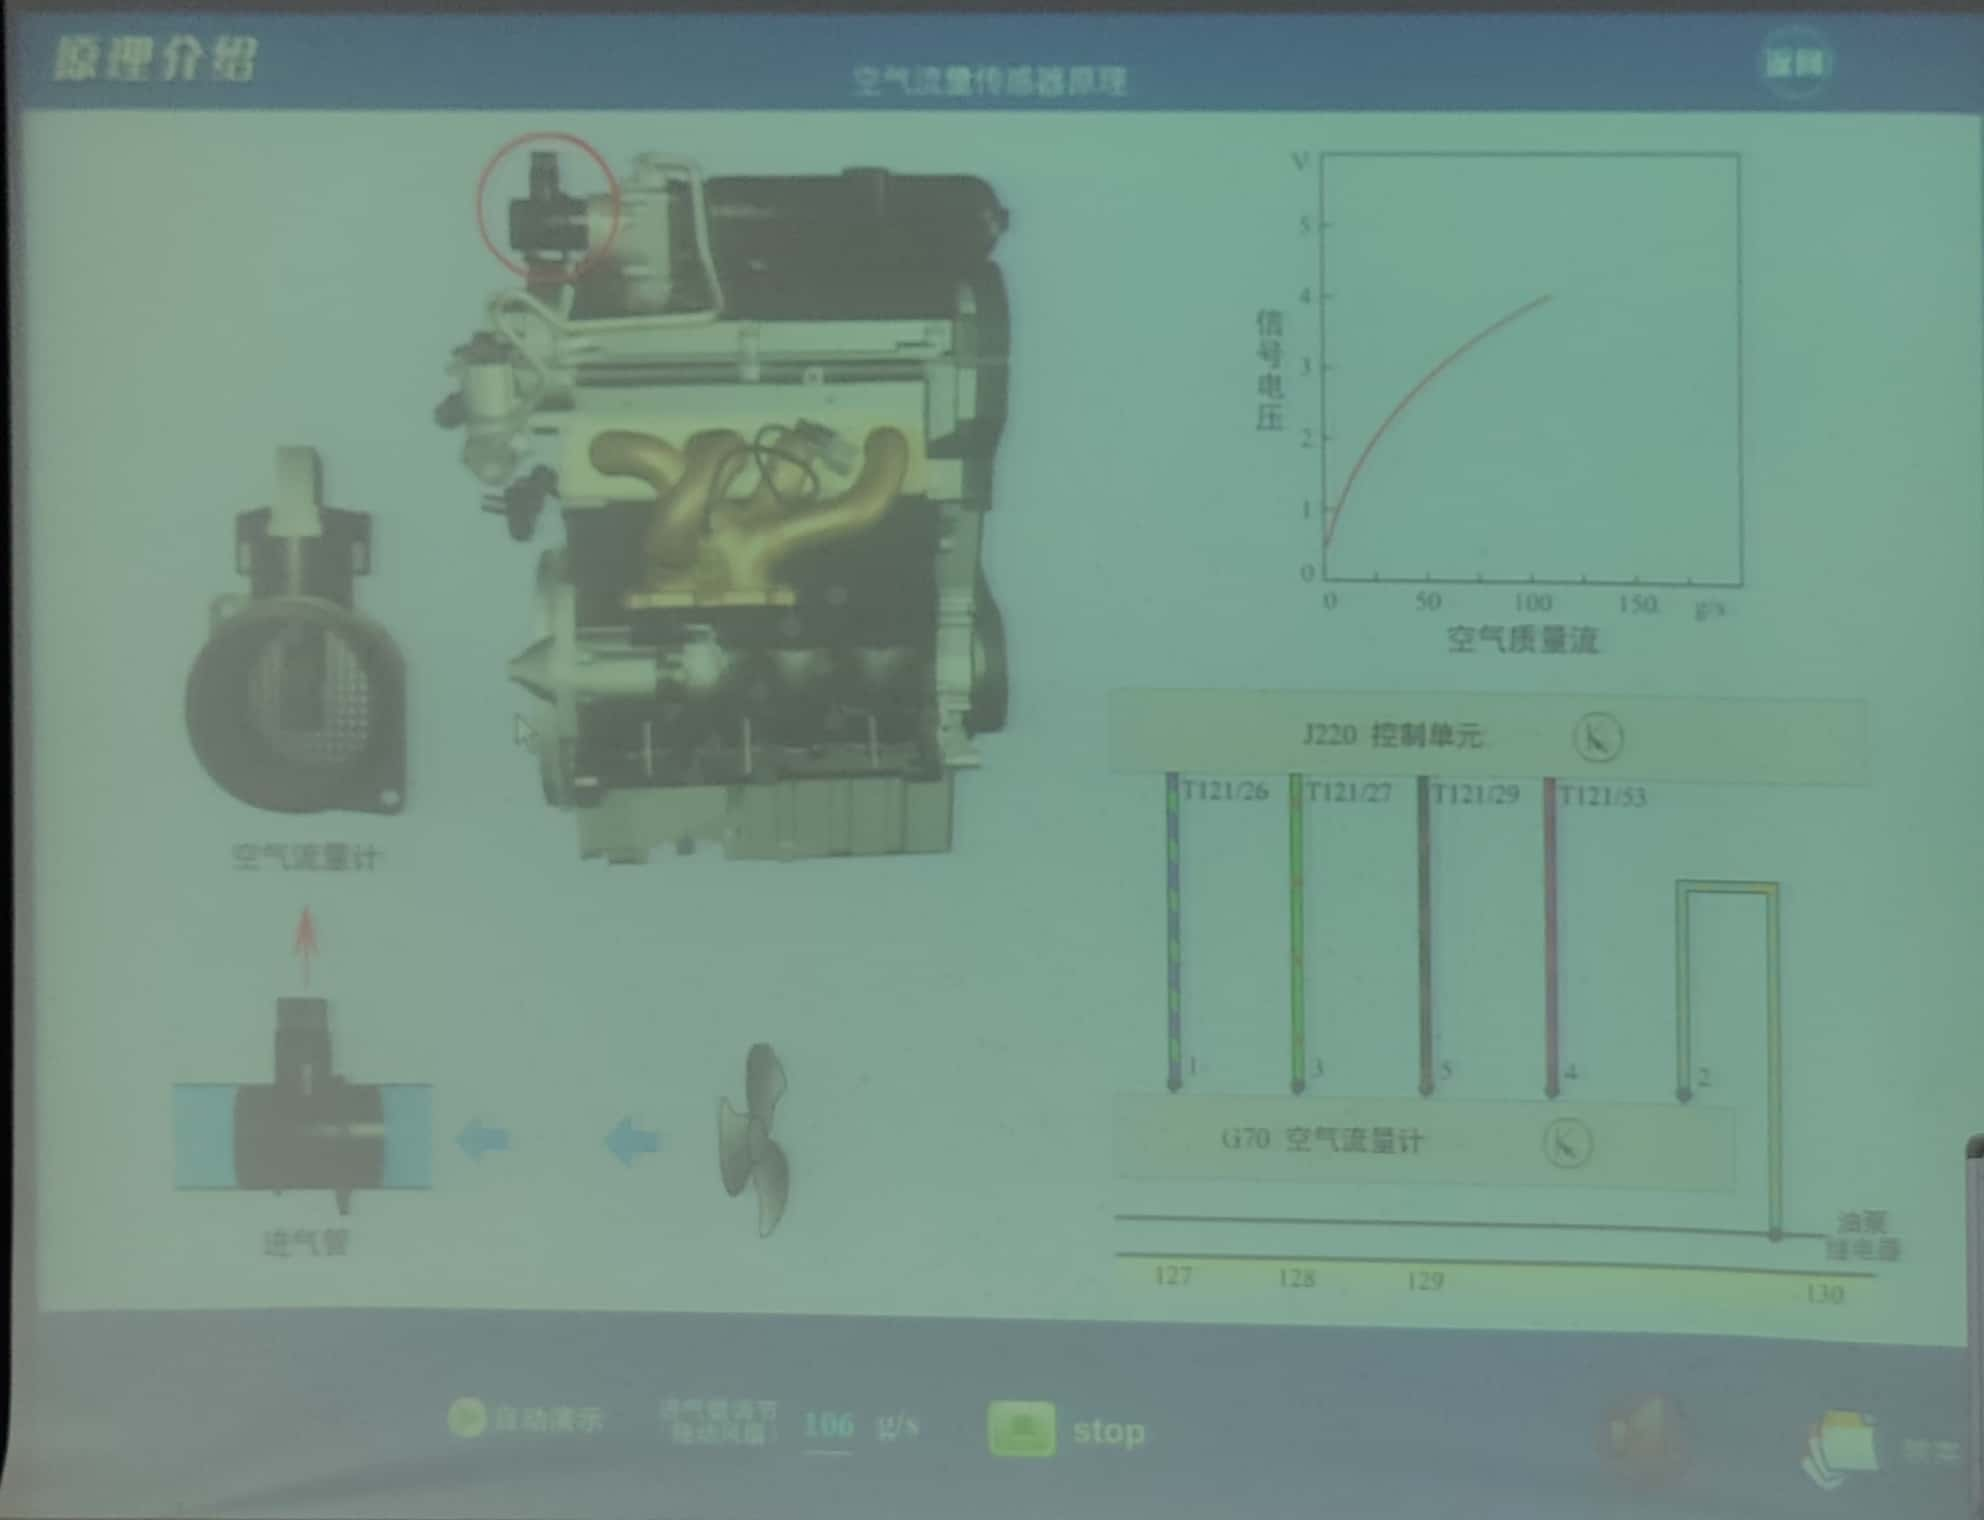
\includegraphics[width=0.45\textwidth]{airflowing sensor}\label{airflowing sensor}}
	\subfigure[前氧传感器]{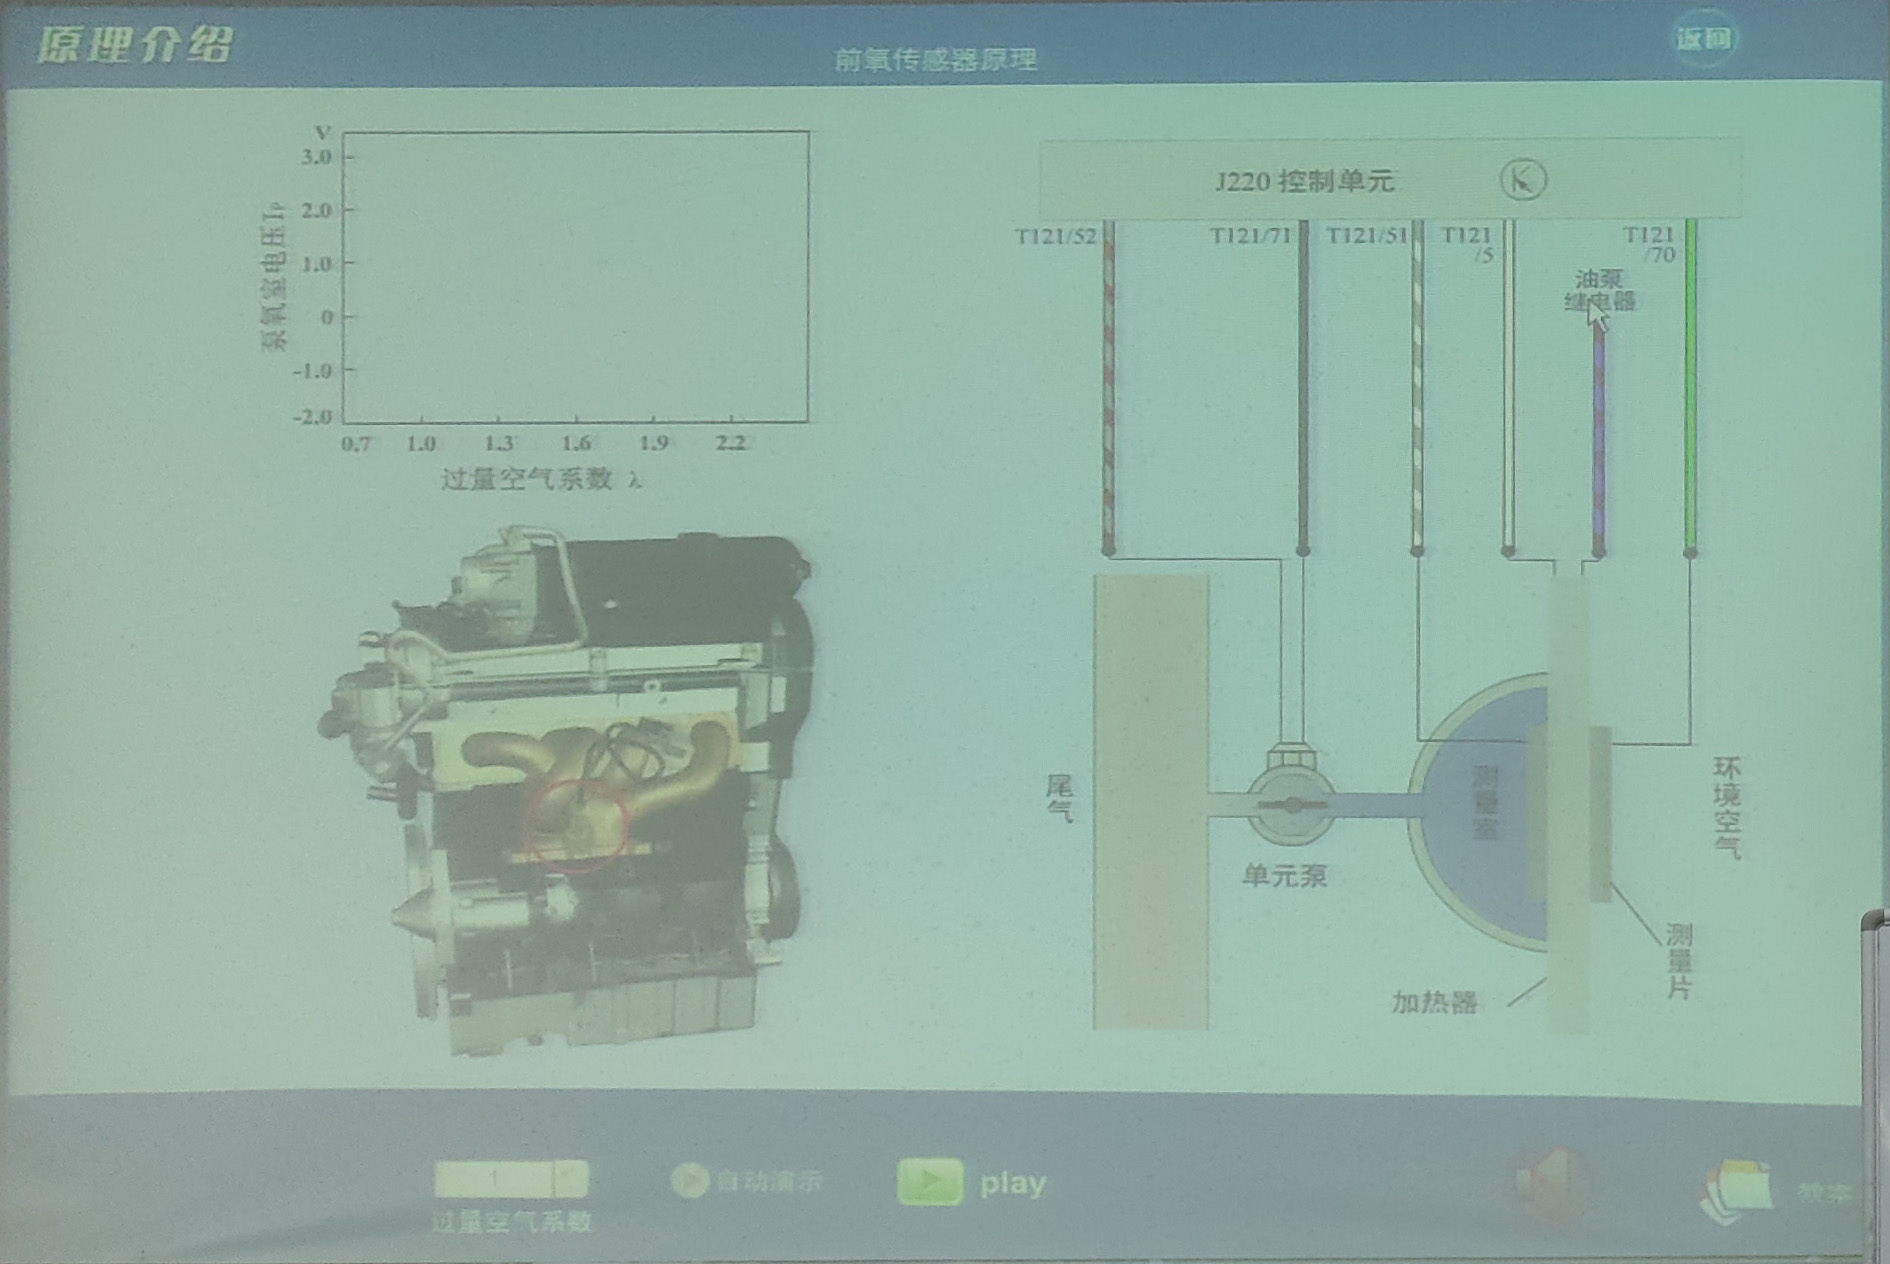
\includegraphics[width=0.45\textwidth]{oxygen sensor F}\label{oxygen sensor F}}
	\subfigure[后氧传感器]{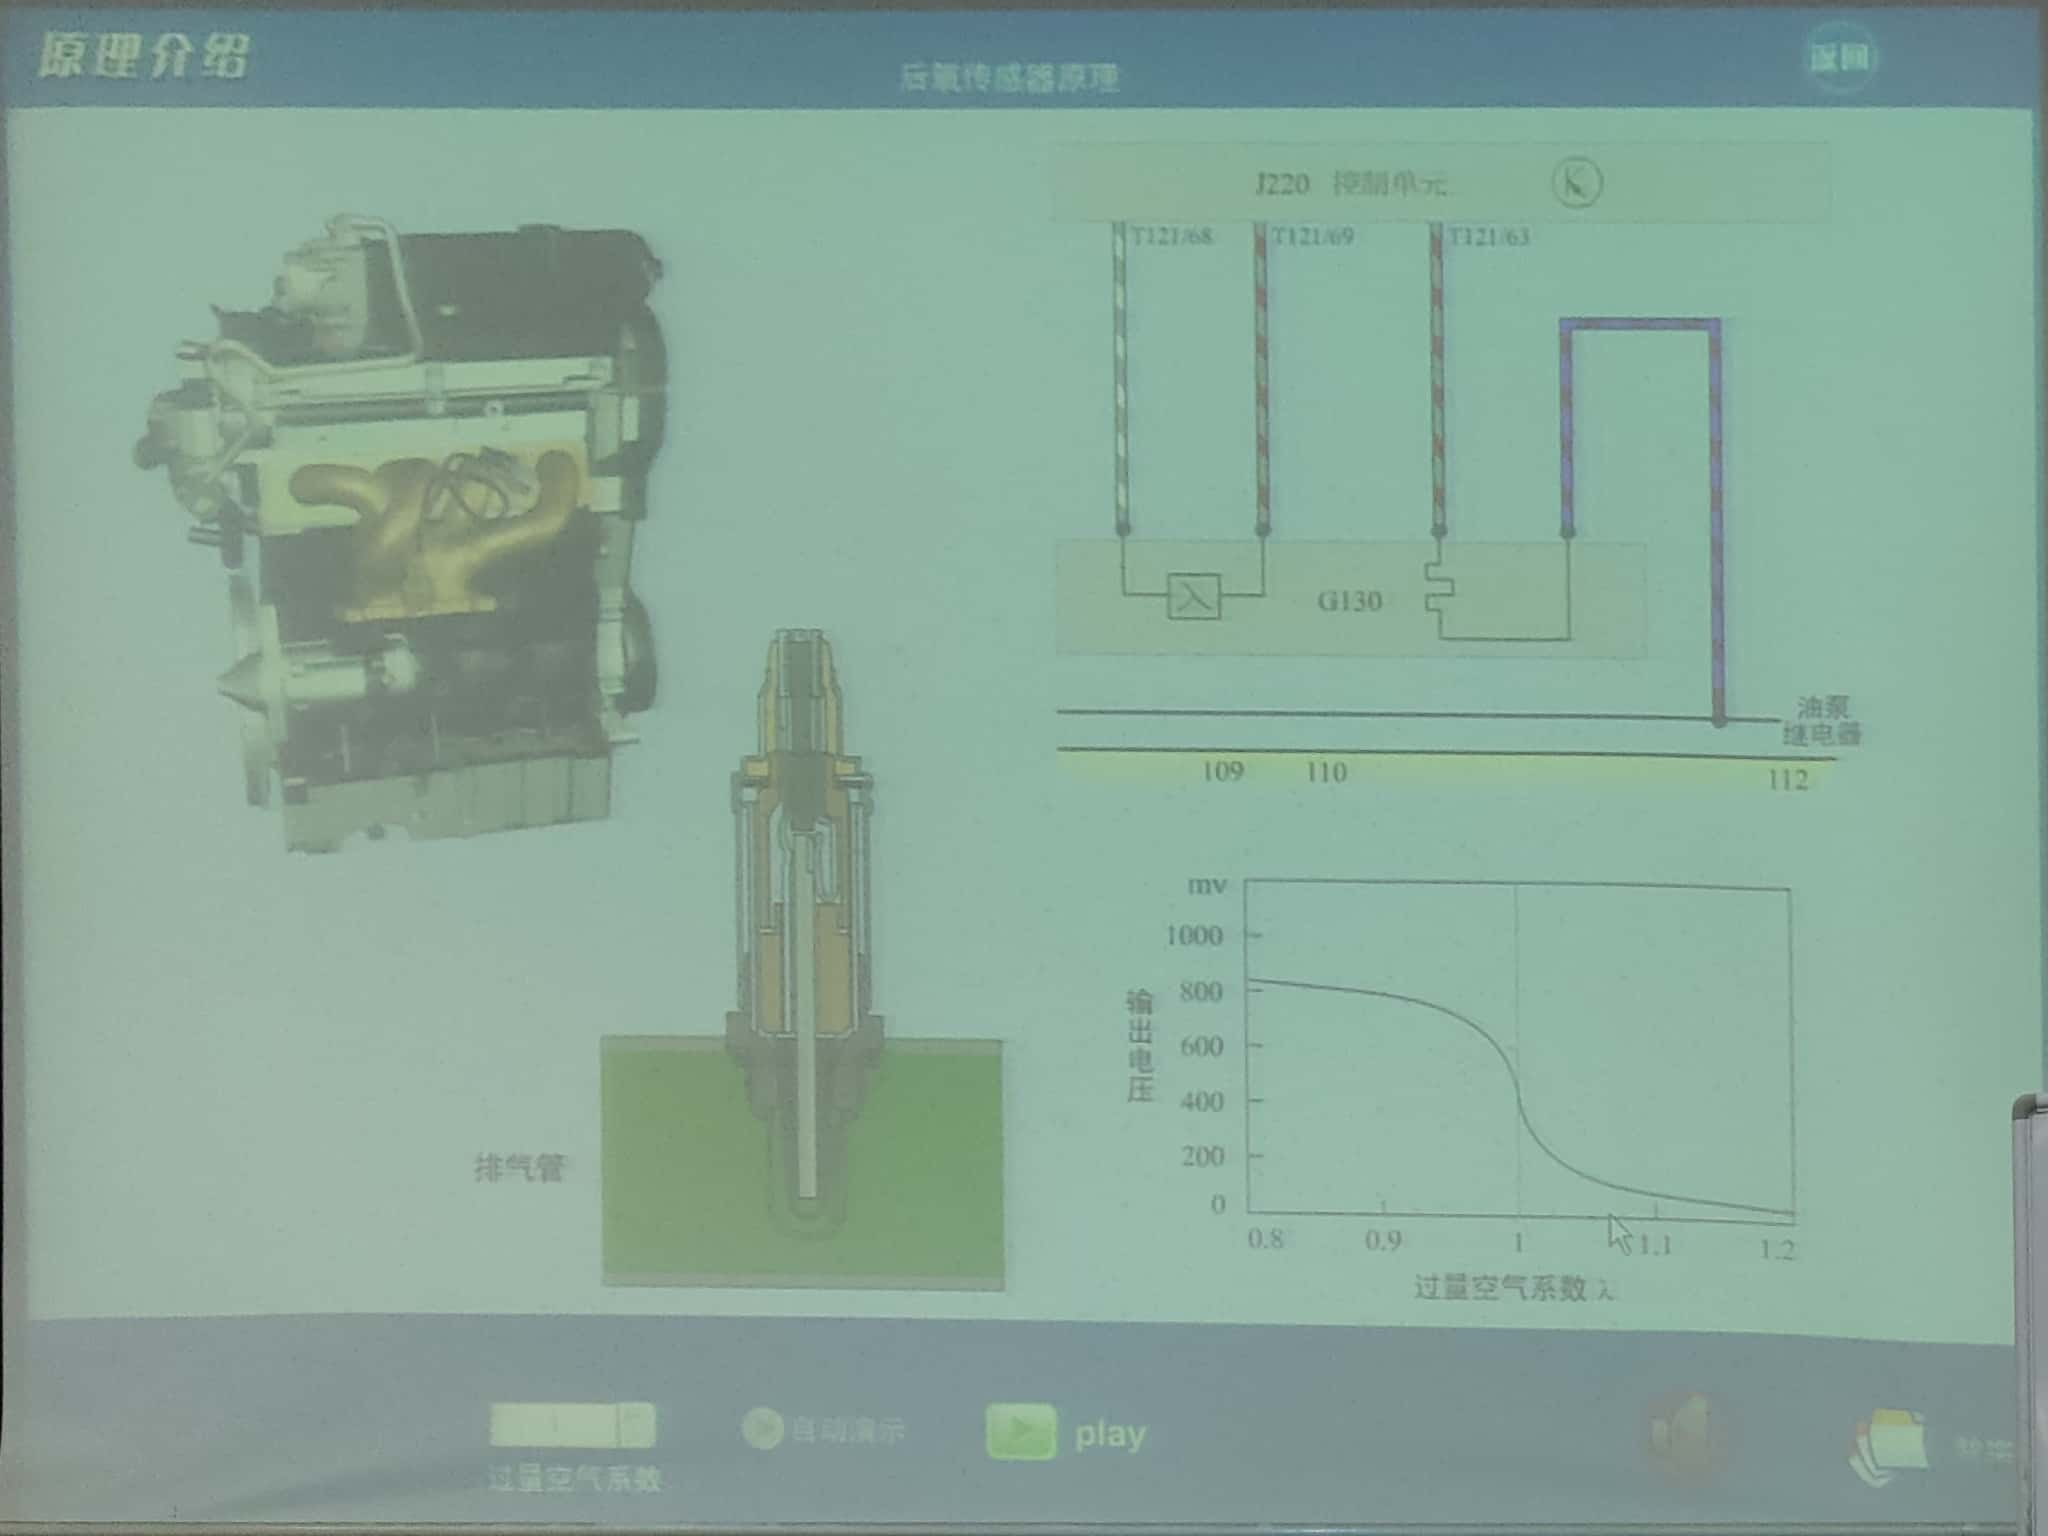
\includegraphics[width=0.45\textwidth]{oxygen sensor B}\label{oxygen sensor B}}
	\subfigure[冷却液温度传感器]{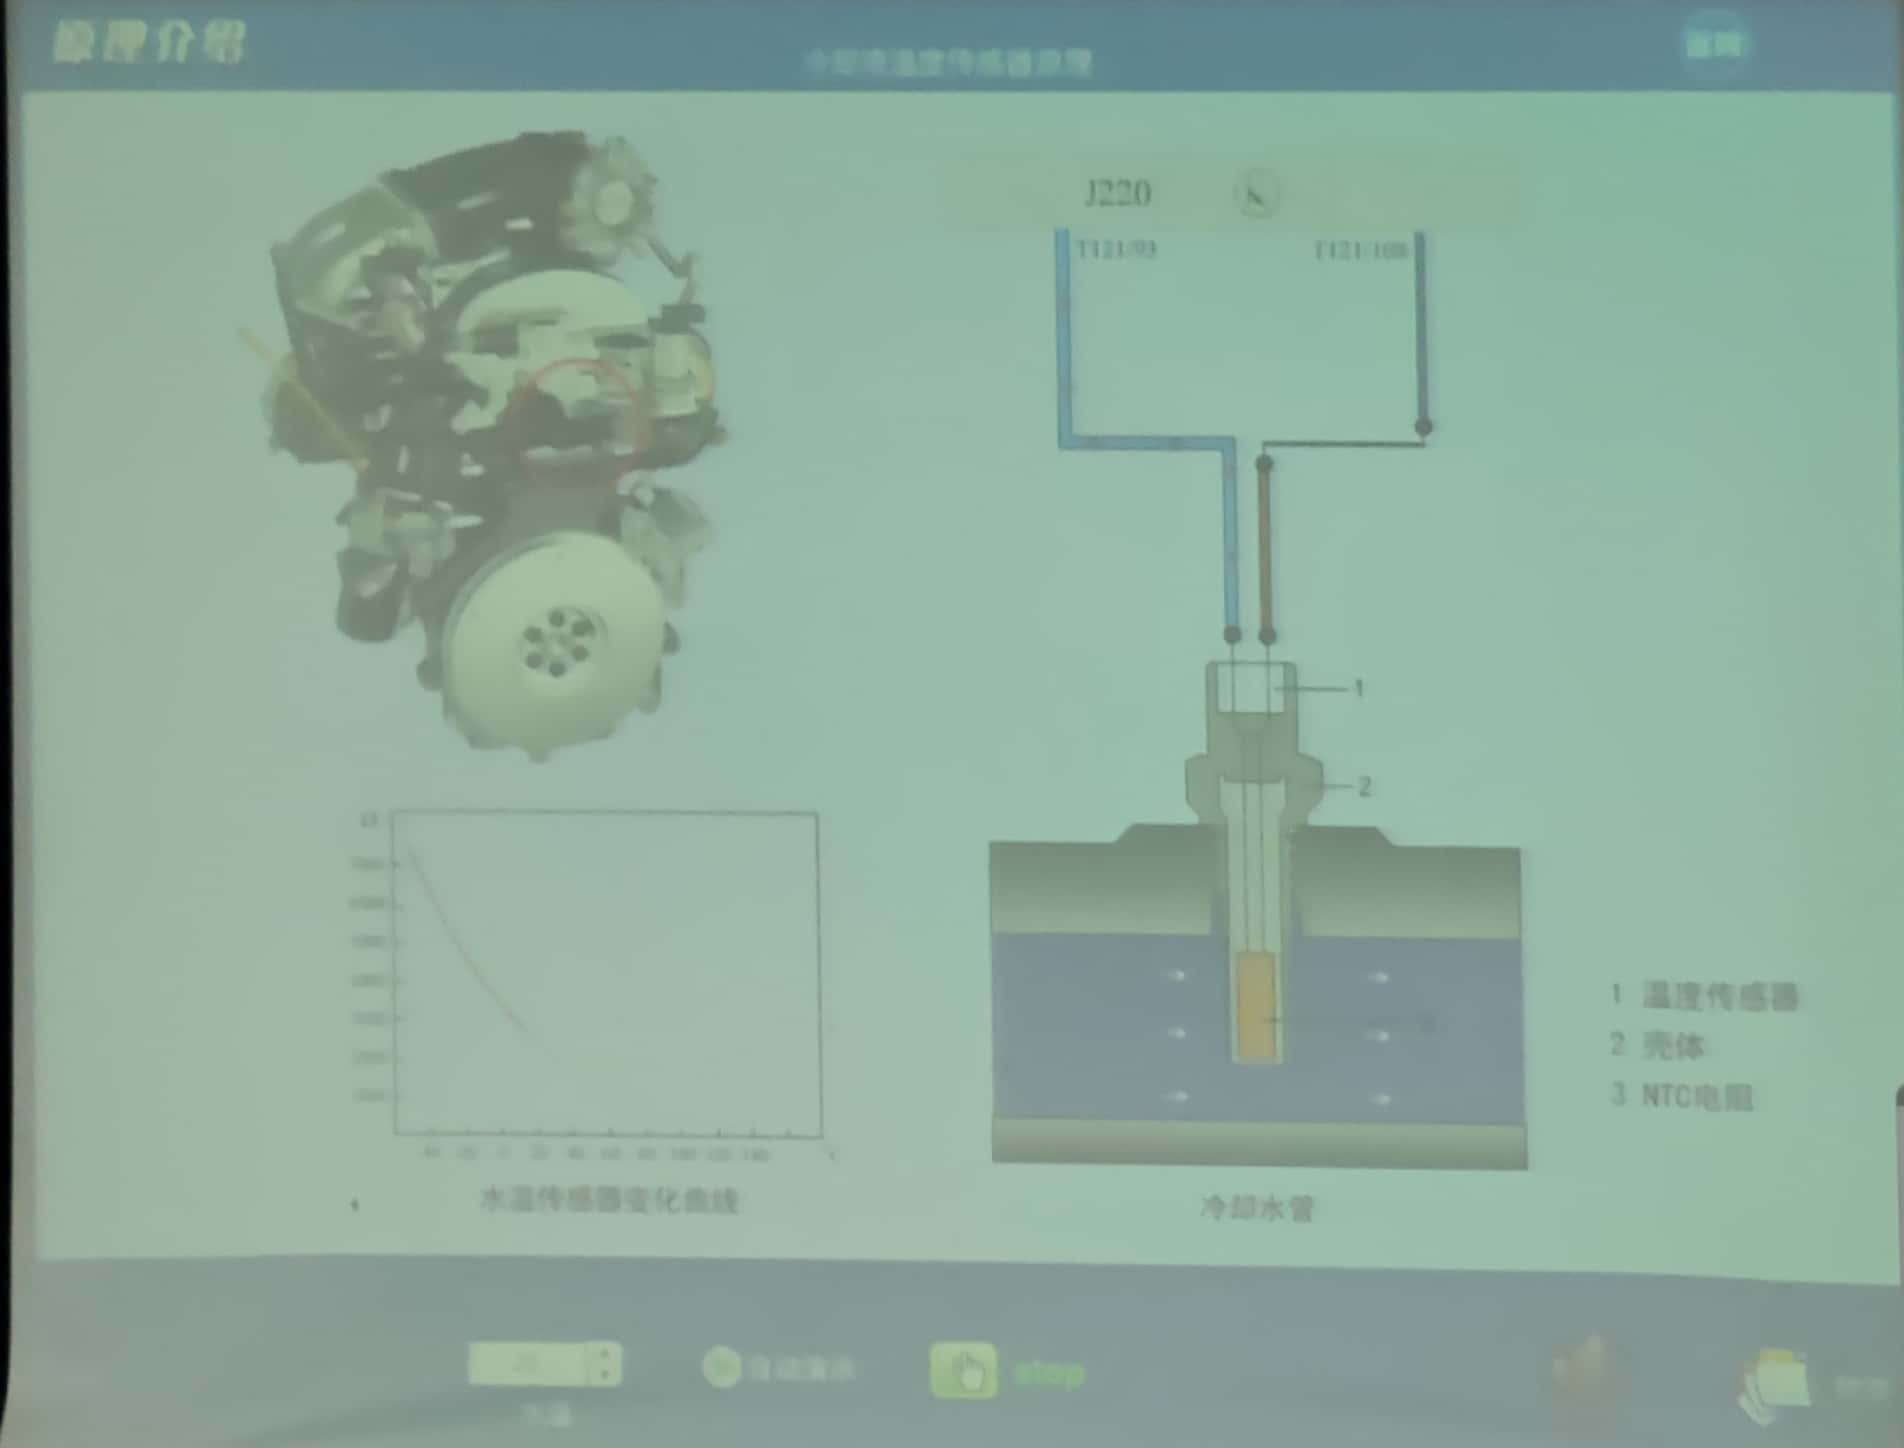
\includegraphics[width=0.45\textwidth]{coolant temperature sensor}\label{coolant temperature sensor}}
	\caption{发动机的控制系统中的部分传感器}
	\label{sensors}
\end{figure}

燃油泵继电器、燃油泵、喷油器、油箱等都是燃油供给系统(\cref{fuel-supplying system})的组成部分。对于缸内直喷汽油机,供油压力都很高,达到\qtyrange[range-phrase = $\,\sim\,$, range-units = single]{300}{450}{\kPa},需采用高压油轨,油轨中压力在发动机运转时变化不大,ECU对喷油器的控制主要是控制其喷油时刻和喷油持续时间。燃油泵继电器只在起动时和发动机运转时接通电动燃油泵,提供足够的燃油压力和富余燃油;当发动机发生事故而停止运转时,燃油泵也停止运转,降低起火风险。油箱内因汽油蒸发产生的高压蒸气通到碳罐(\cref{charcoal canister})中,碳罐底部接大气,上部一边接油箱一边接进气管,ECU在需要时开启碳罐控制阀,燃油蒸气在压力差的作用下被导入到进气管中,随后进入汽缸中燃烧。当然,碳罐系统的存在也使得燃油供给量不完全由喷油量控制,且经过碳罐的蒸气量不便计量,这也是需要设置氧传感器进行$\lambda$闭环控制的原因之一。

点火系统要能保证按时并提供足量能量点燃燃烧室内混合气。最佳点火提前角受很多因素影响,其中最主要的是发动机转速和混合气的燃烧速度,而混合气的燃烧速度又和混合气的成分、发动机的结构(包括燃烧室形状和压缩比)等有关。当发动机转速一定时,随着负荷(节气门开度)的增加,进入汽缸的可燃混合气增多,压缩终了时的压力和温度升高,同时残余废气在缸内混合气中所占的比例下降,混合气燃烧速度增大,点火提前角应适当减小;反之负荷减小时点火提前角应加大。当节气门开度一定时,发动机转速升高,燃烧过程所占曲轴转角增大,应适当加大点火提前角,否则燃烧会延续到做功冲程使得功率和经济性下降。对于抗爆性较好的汽油,许用的点火提前角较大,加注不同牌号的汽油后点火提前角也应相应调节。ECU确定点火提前角后,发出信号令点火系统点火。电控点火系统分为有分电器式和无分电器式两种,现在用的多为无分电器点火系统,又称直接点火系统。直接点火系统又有单火花点火线圈、双火花点火线圈和四火花点火线圈等,\cref{ignition system}所示为双火花点火线圈,1、4缸和2、3缸分别同时点火,这样点火时一个汽缸在压缩冲程的上止点附近,另一个汽缸运行到排气冲程上止点附近,但只有一个缸中有可燃混合气,可以被点燃。

\cref{VVT}所示的是一种张紧轮式进气相位调节装置,排气凸轮相位固定,液压缸使链条的上(下)部分张紧且长度发生变化,从而带动进气凸轮相对旋转一角度实现可变气门正时。怠速时,进气门延迟关闭,改善燃烧稳定性;中、低转速时,进气门提前关闭,以获得较大转矩;高转速时,进气门延迟关闭,利用进气惯性提高汽缸充气量以提高功率。

在电子节气门系统(\cref{electronic throttle})中,节气门与加速踏板间无拉索的机械连接,节气门开度完全受ECU控制。当发动机不运转且点火开关打开时,ECU只根据加速踏板位置控制节气门控制器。当发动机运转时,ECU对节气门的控制不完全依赖加速踏板的输入,譬如说可在加速踏板仅踏下一半时即令节气门全开,减少节流损失。有电子节气门的发动机还不需怠速调节器,进气量可精确控制,在提升车辆驾驶性能的同时降低排放和油耗。

二次空气系统(\cref{secondary air})和排气再循环系统(\cref{EGR})都是发动机排放控制系统的一部分,现代发动机管理系统将喷油控制和排放控制作为统一的整体,以满足日趋严格的排放法规。二次空气系统主要在发动机冷起动和暖机过程中工作,在每缸排气门后面导入空气,使得高温废气中的\ce{HC}和\ce{CO}在排气管中继续燃烧,产生热量让催化转换器尽快升温。排气再循环系统通过回引部分废气与新鲜空气一起参与燃烧,降低混合气中\ce{O2}含量和燃烧温度从而抑制\ce{NO_x}的产生。

正如\cref{subsection:1.1}所提到的那样,废气涡轮增压系统(\cref{turbocharging})上的放气阀也受ECU控制。

\begin{figure}[htbp]
	\centering
	\subfigure[燃油供给系统]{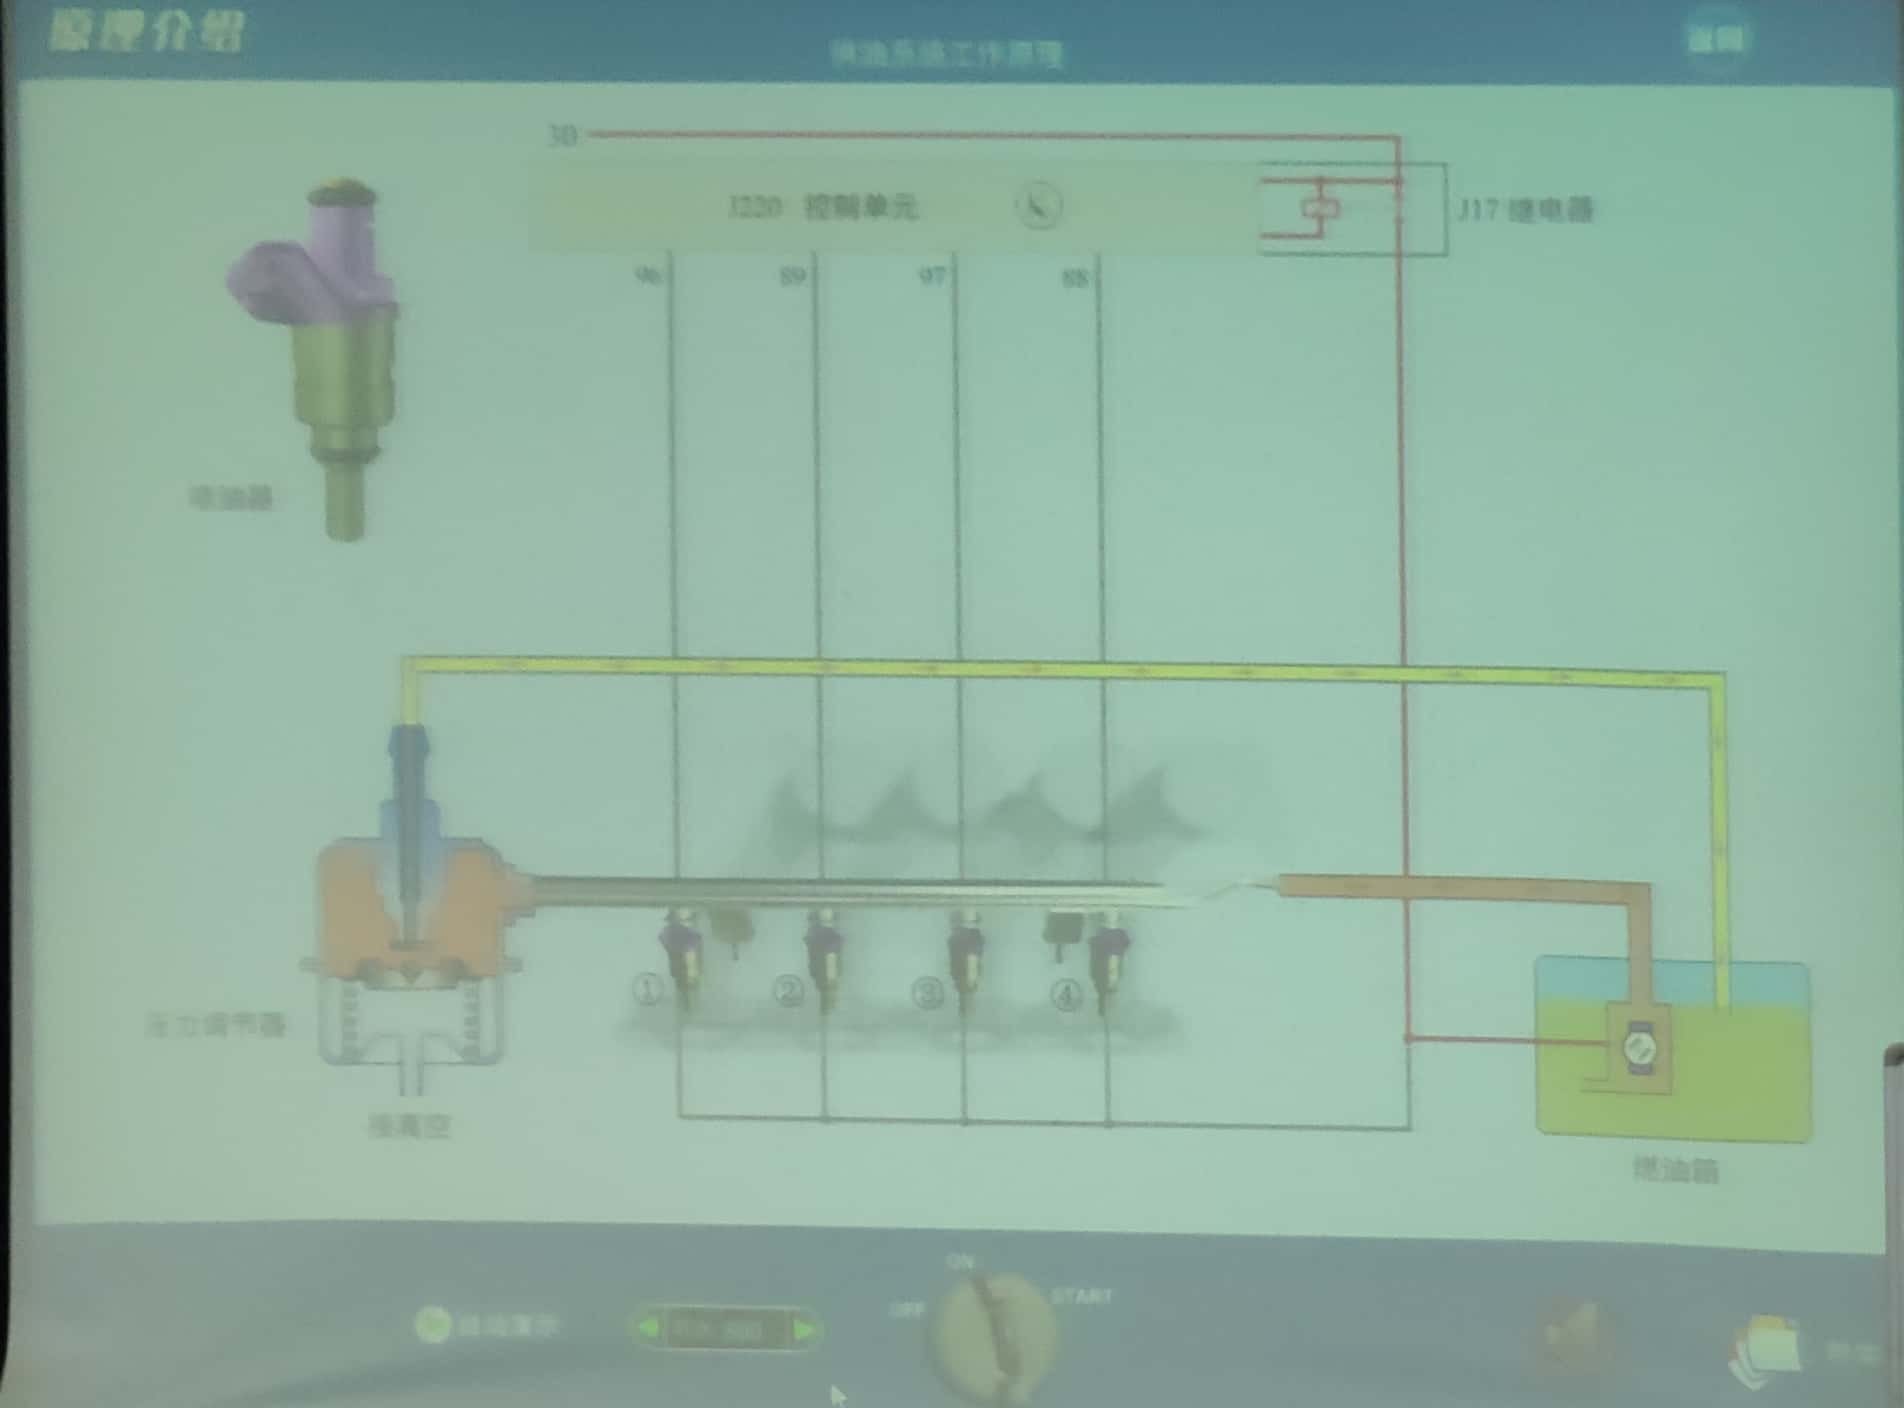
\includegraphics[width=0.3\textwidth]{fuel-supplying system}\label{fuel-supplying system}}
	\subfigure[碳罐]{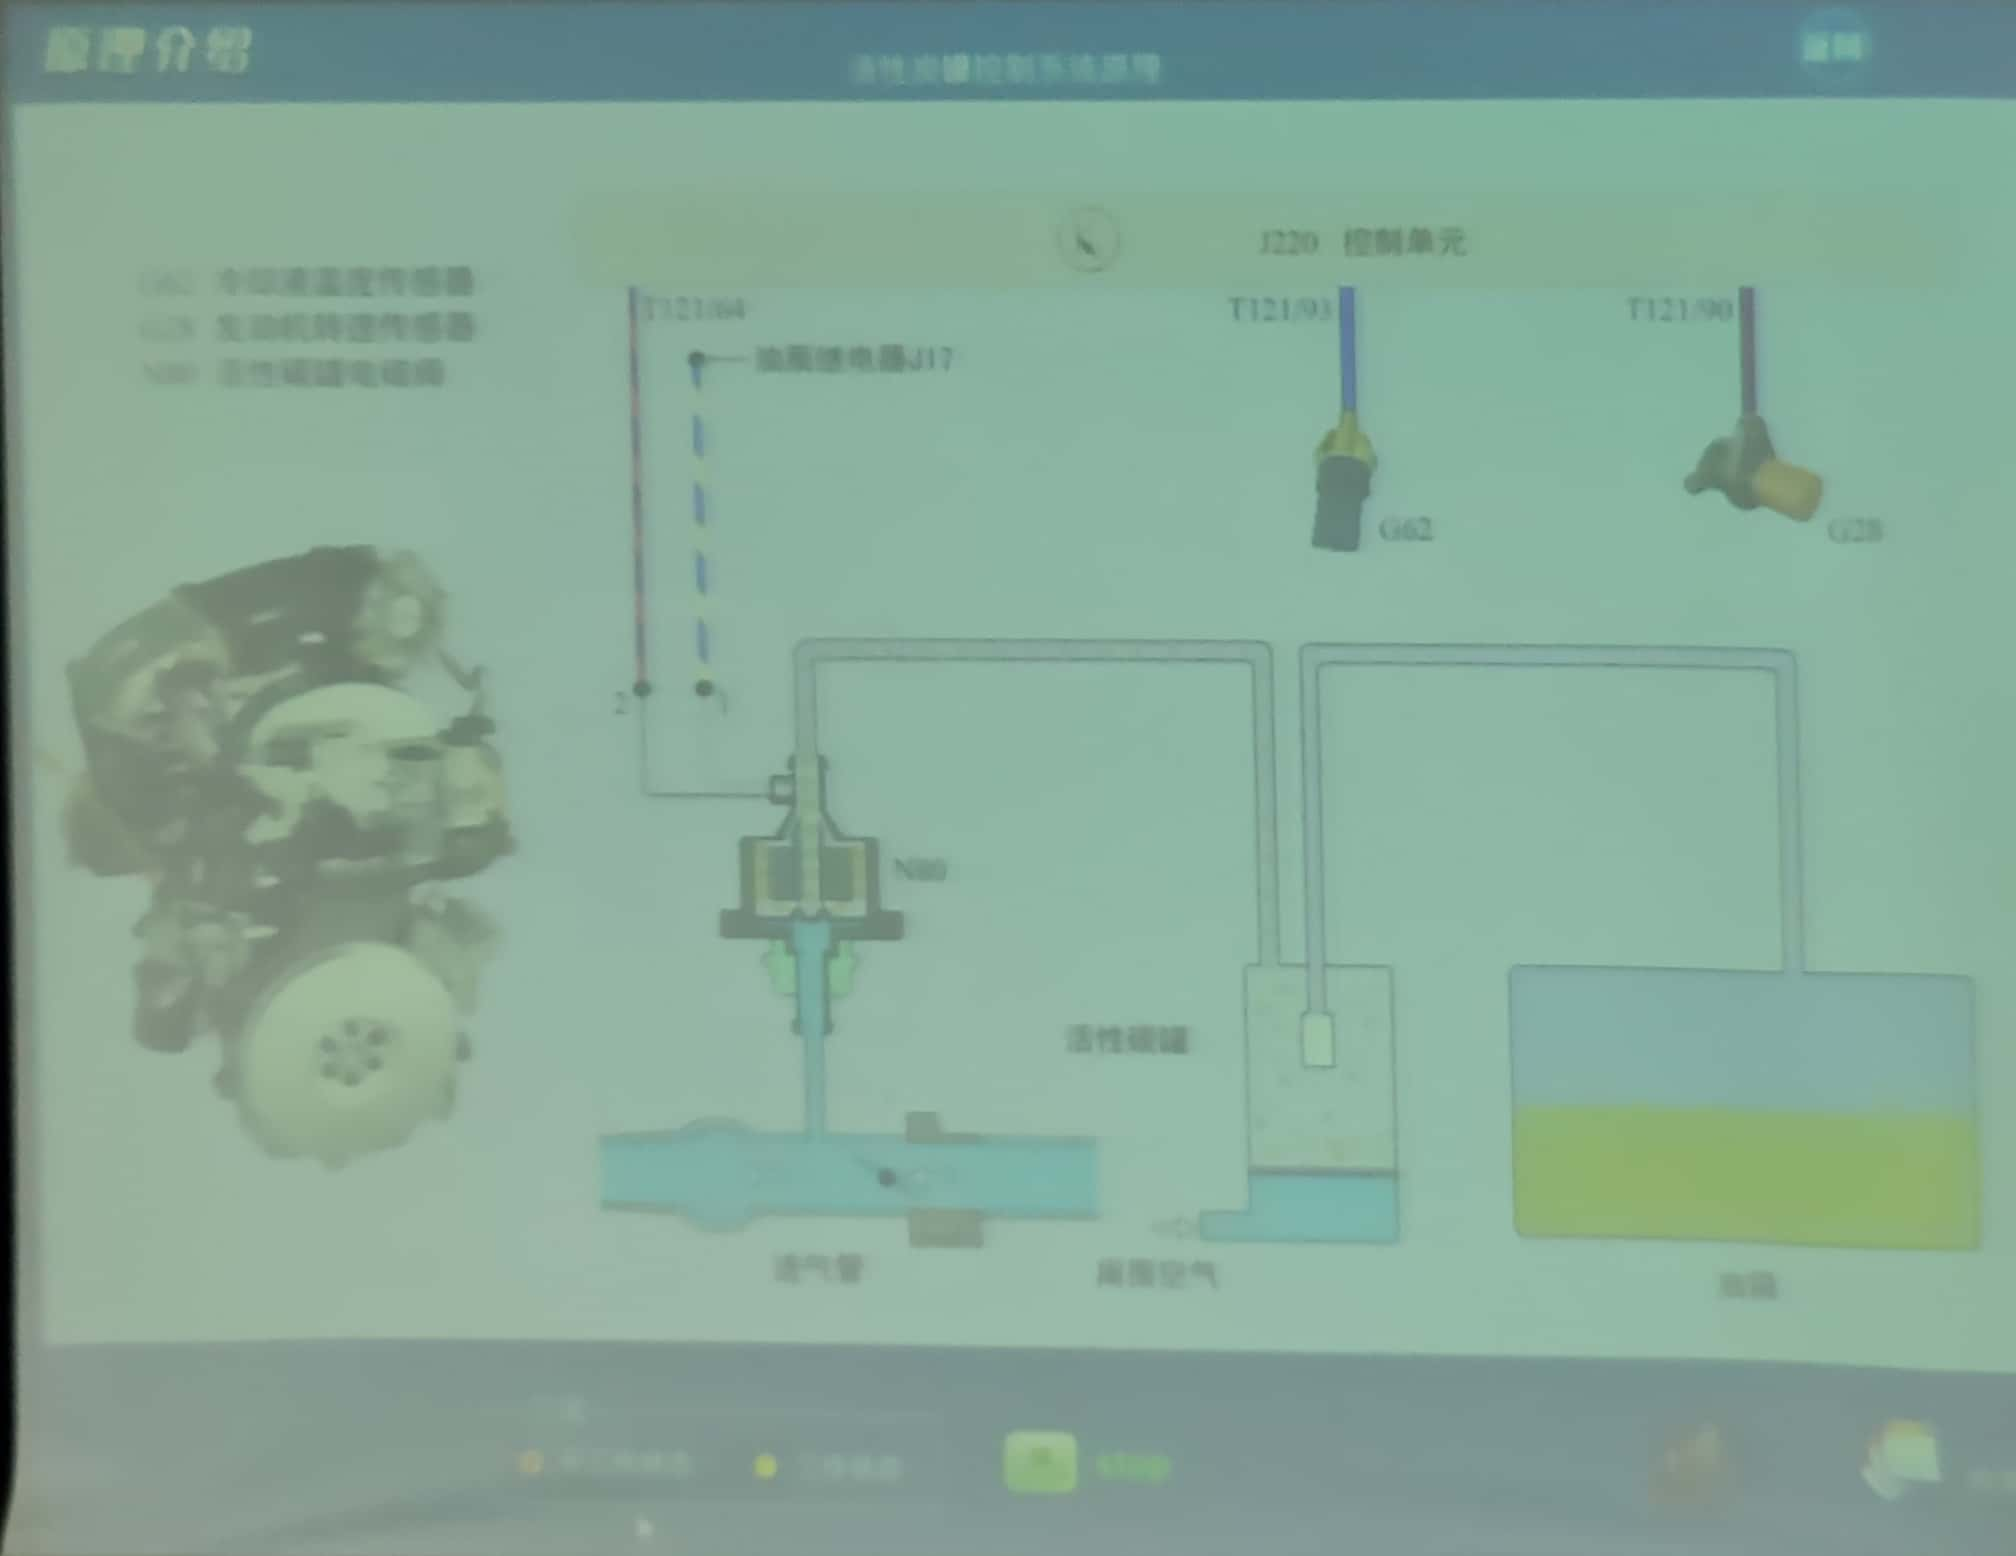
\includegraphics[width=0.3\textwidth]{charcoal canister}\label{charcoal canister}}
	\subfigure[点火系统]{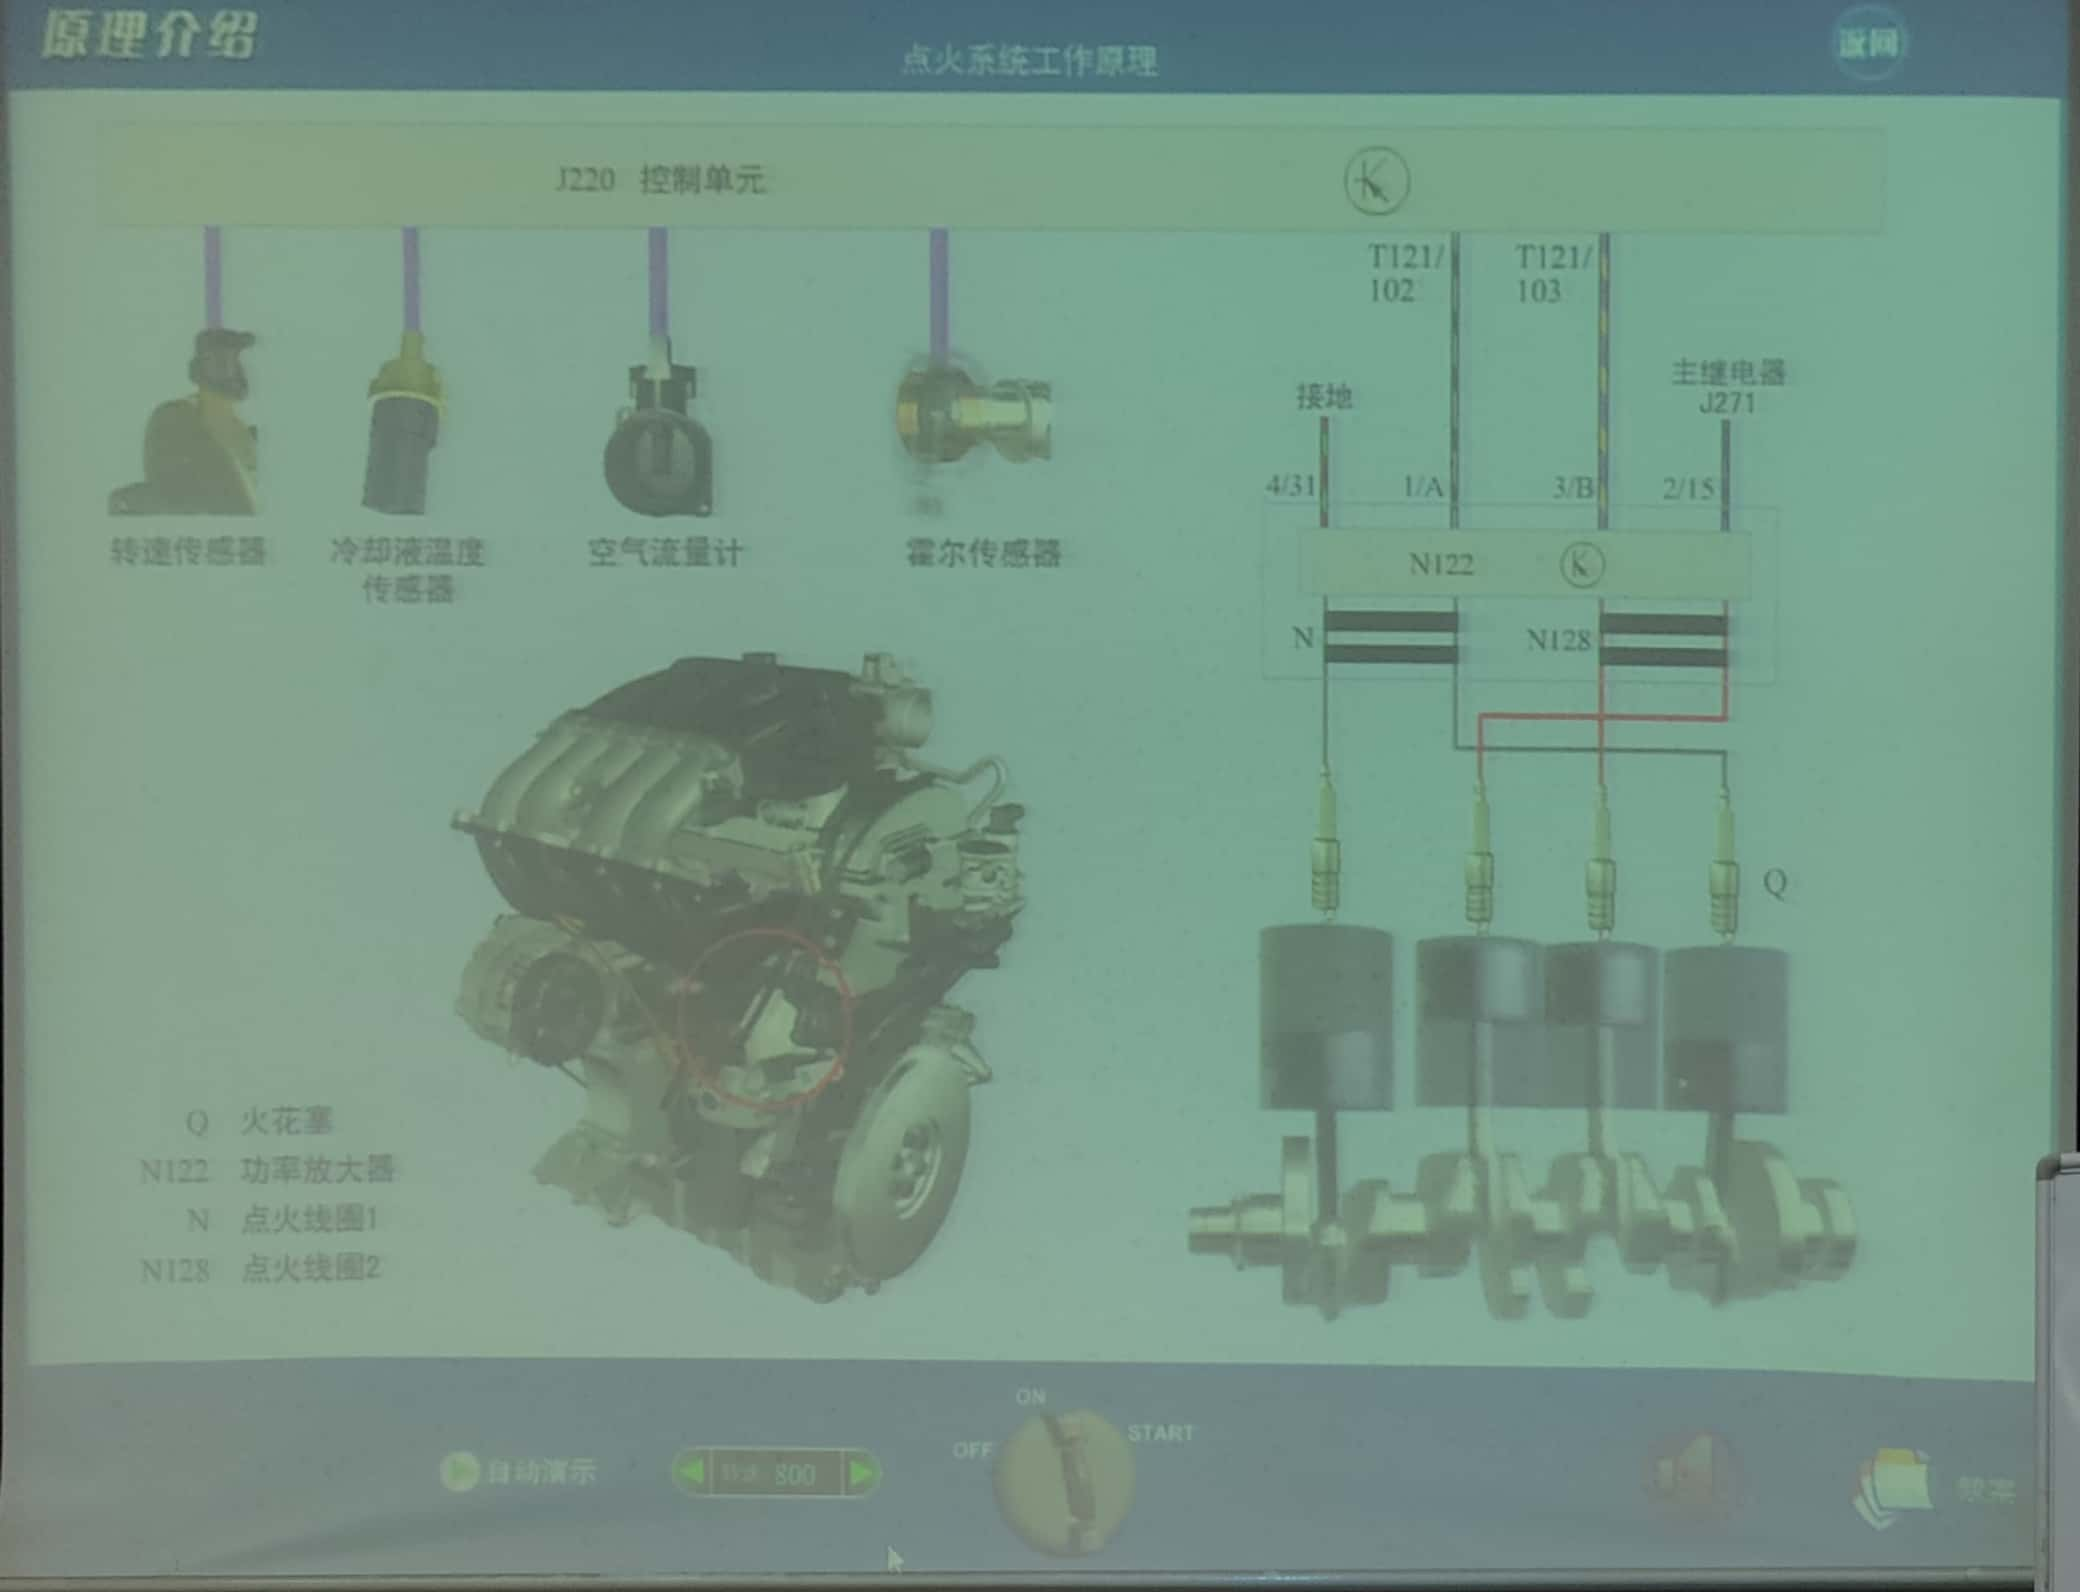
\includegraphics[width=0.3\textwidth]{ignition system}\label{ignition system}}
	\subfigure[可变气门正时]{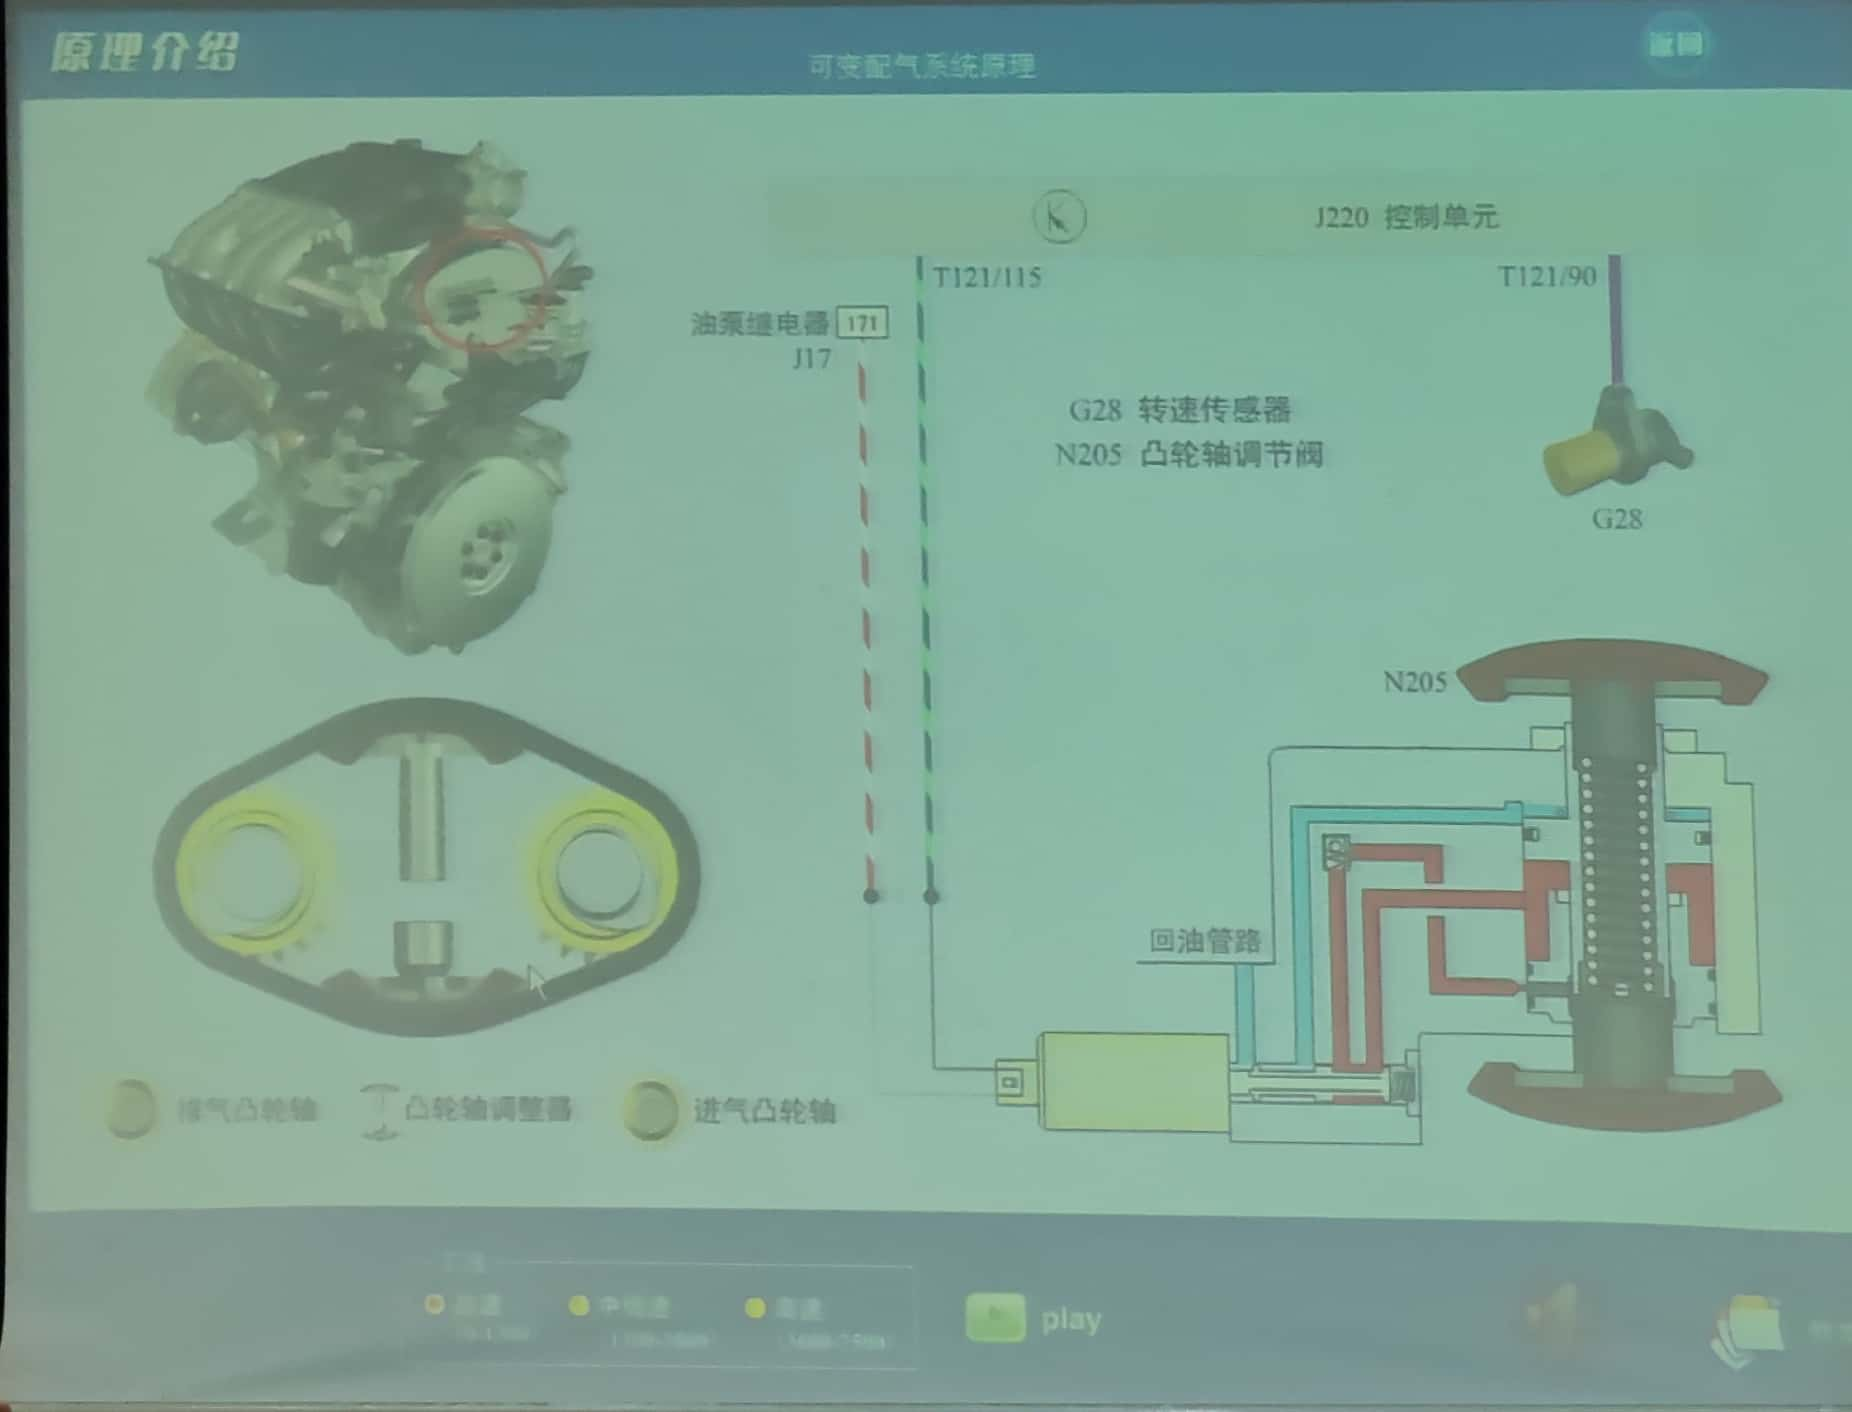
\includegraphics[width=0.3\textwidth]{VVT}\label{VVT}}
	\subfigure[电子油门]{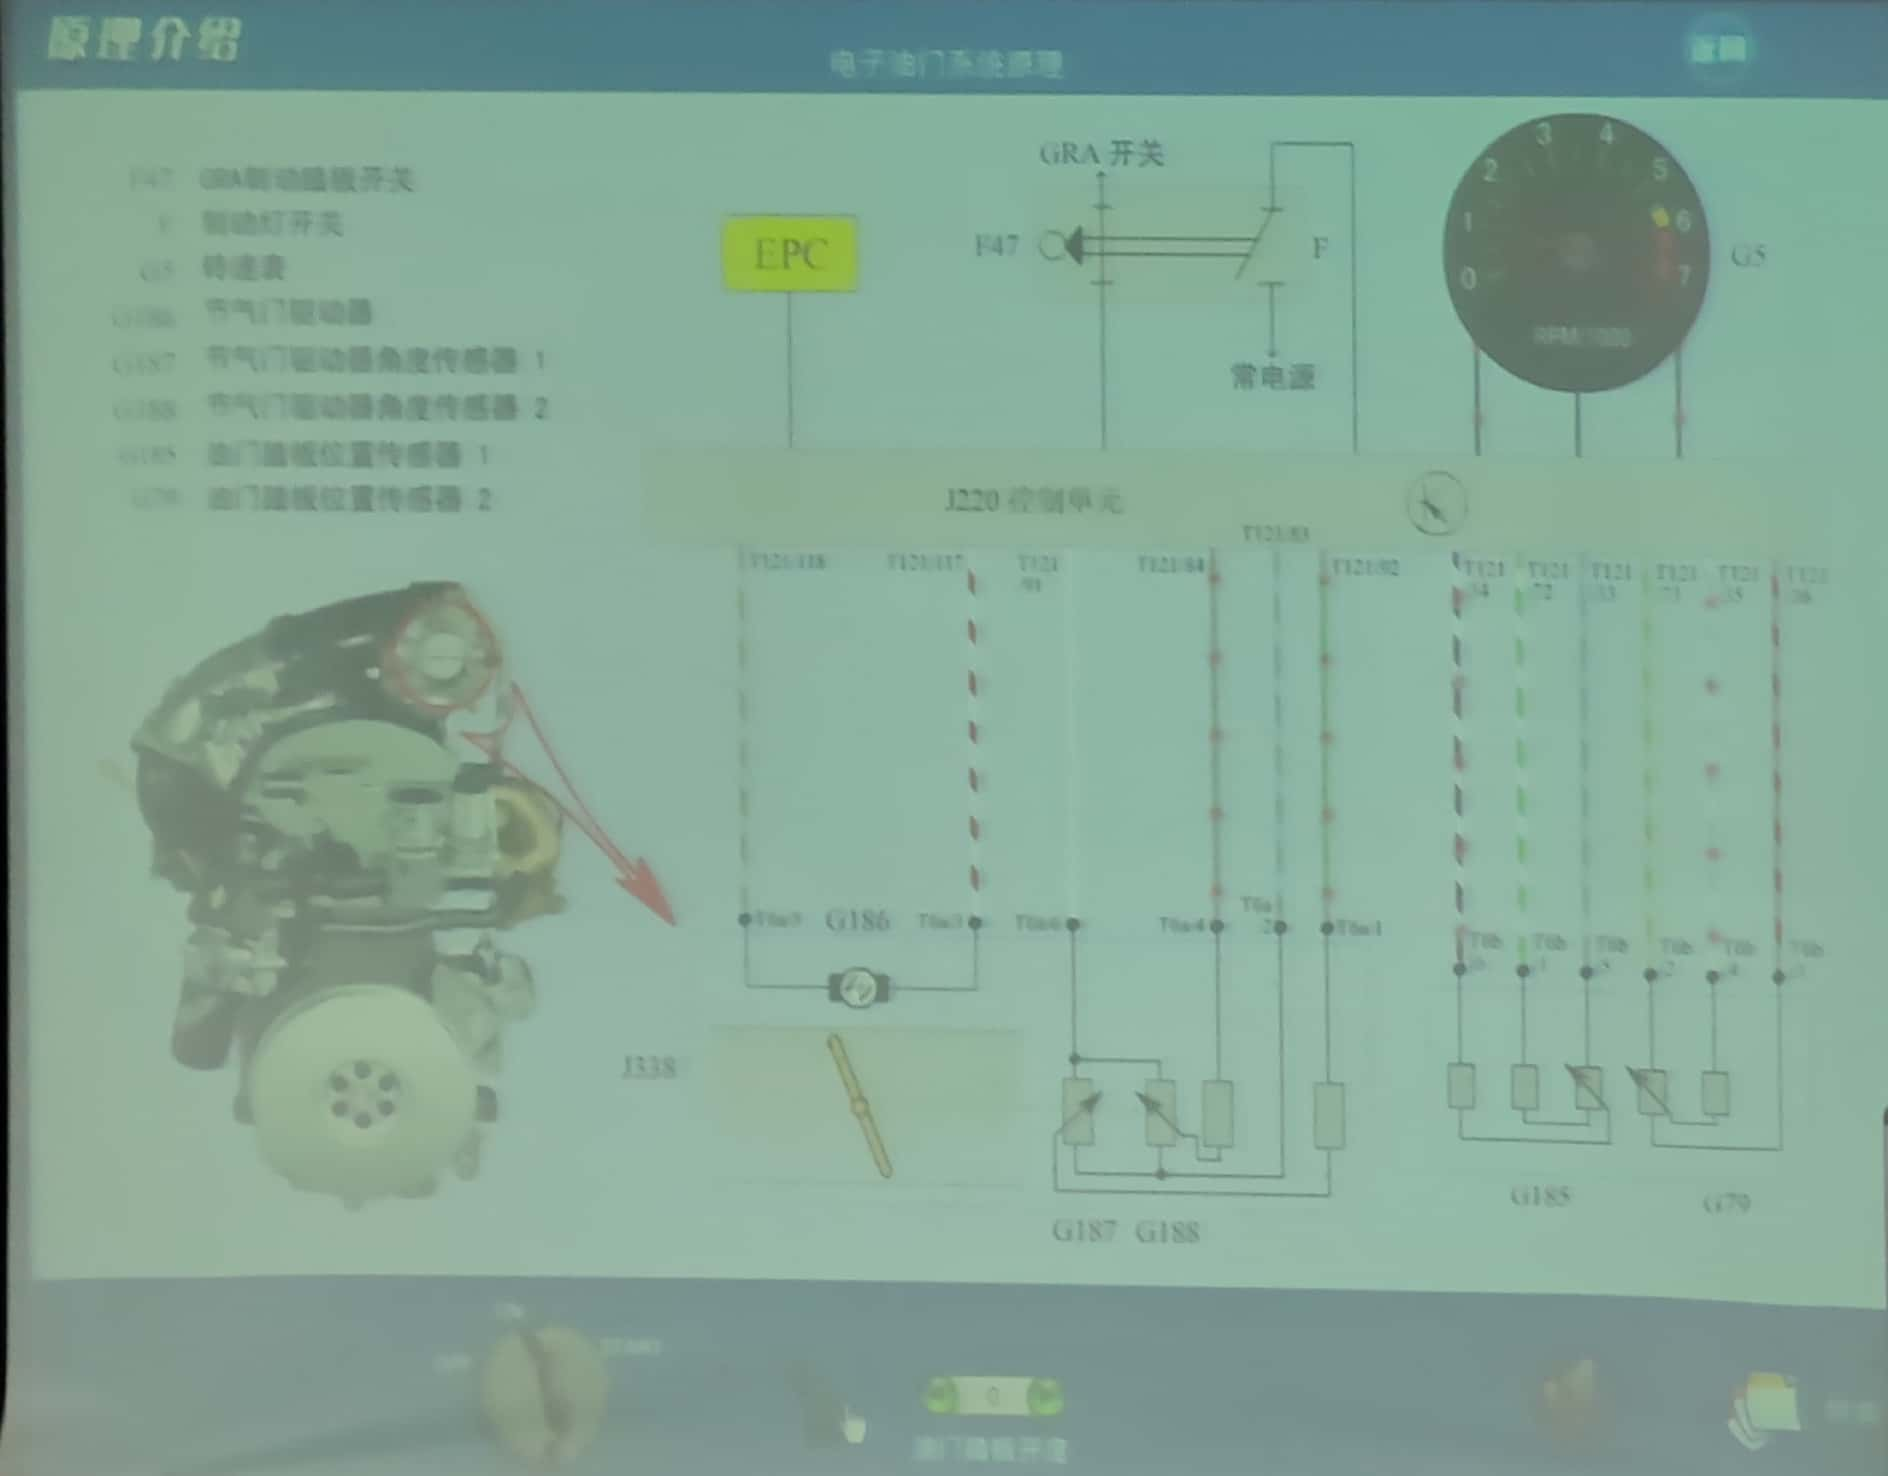
\includegraphics[width=0.3\textwidth]{electronic throttle}\label{electronic throttle}}
	\subfigure[二次空气]{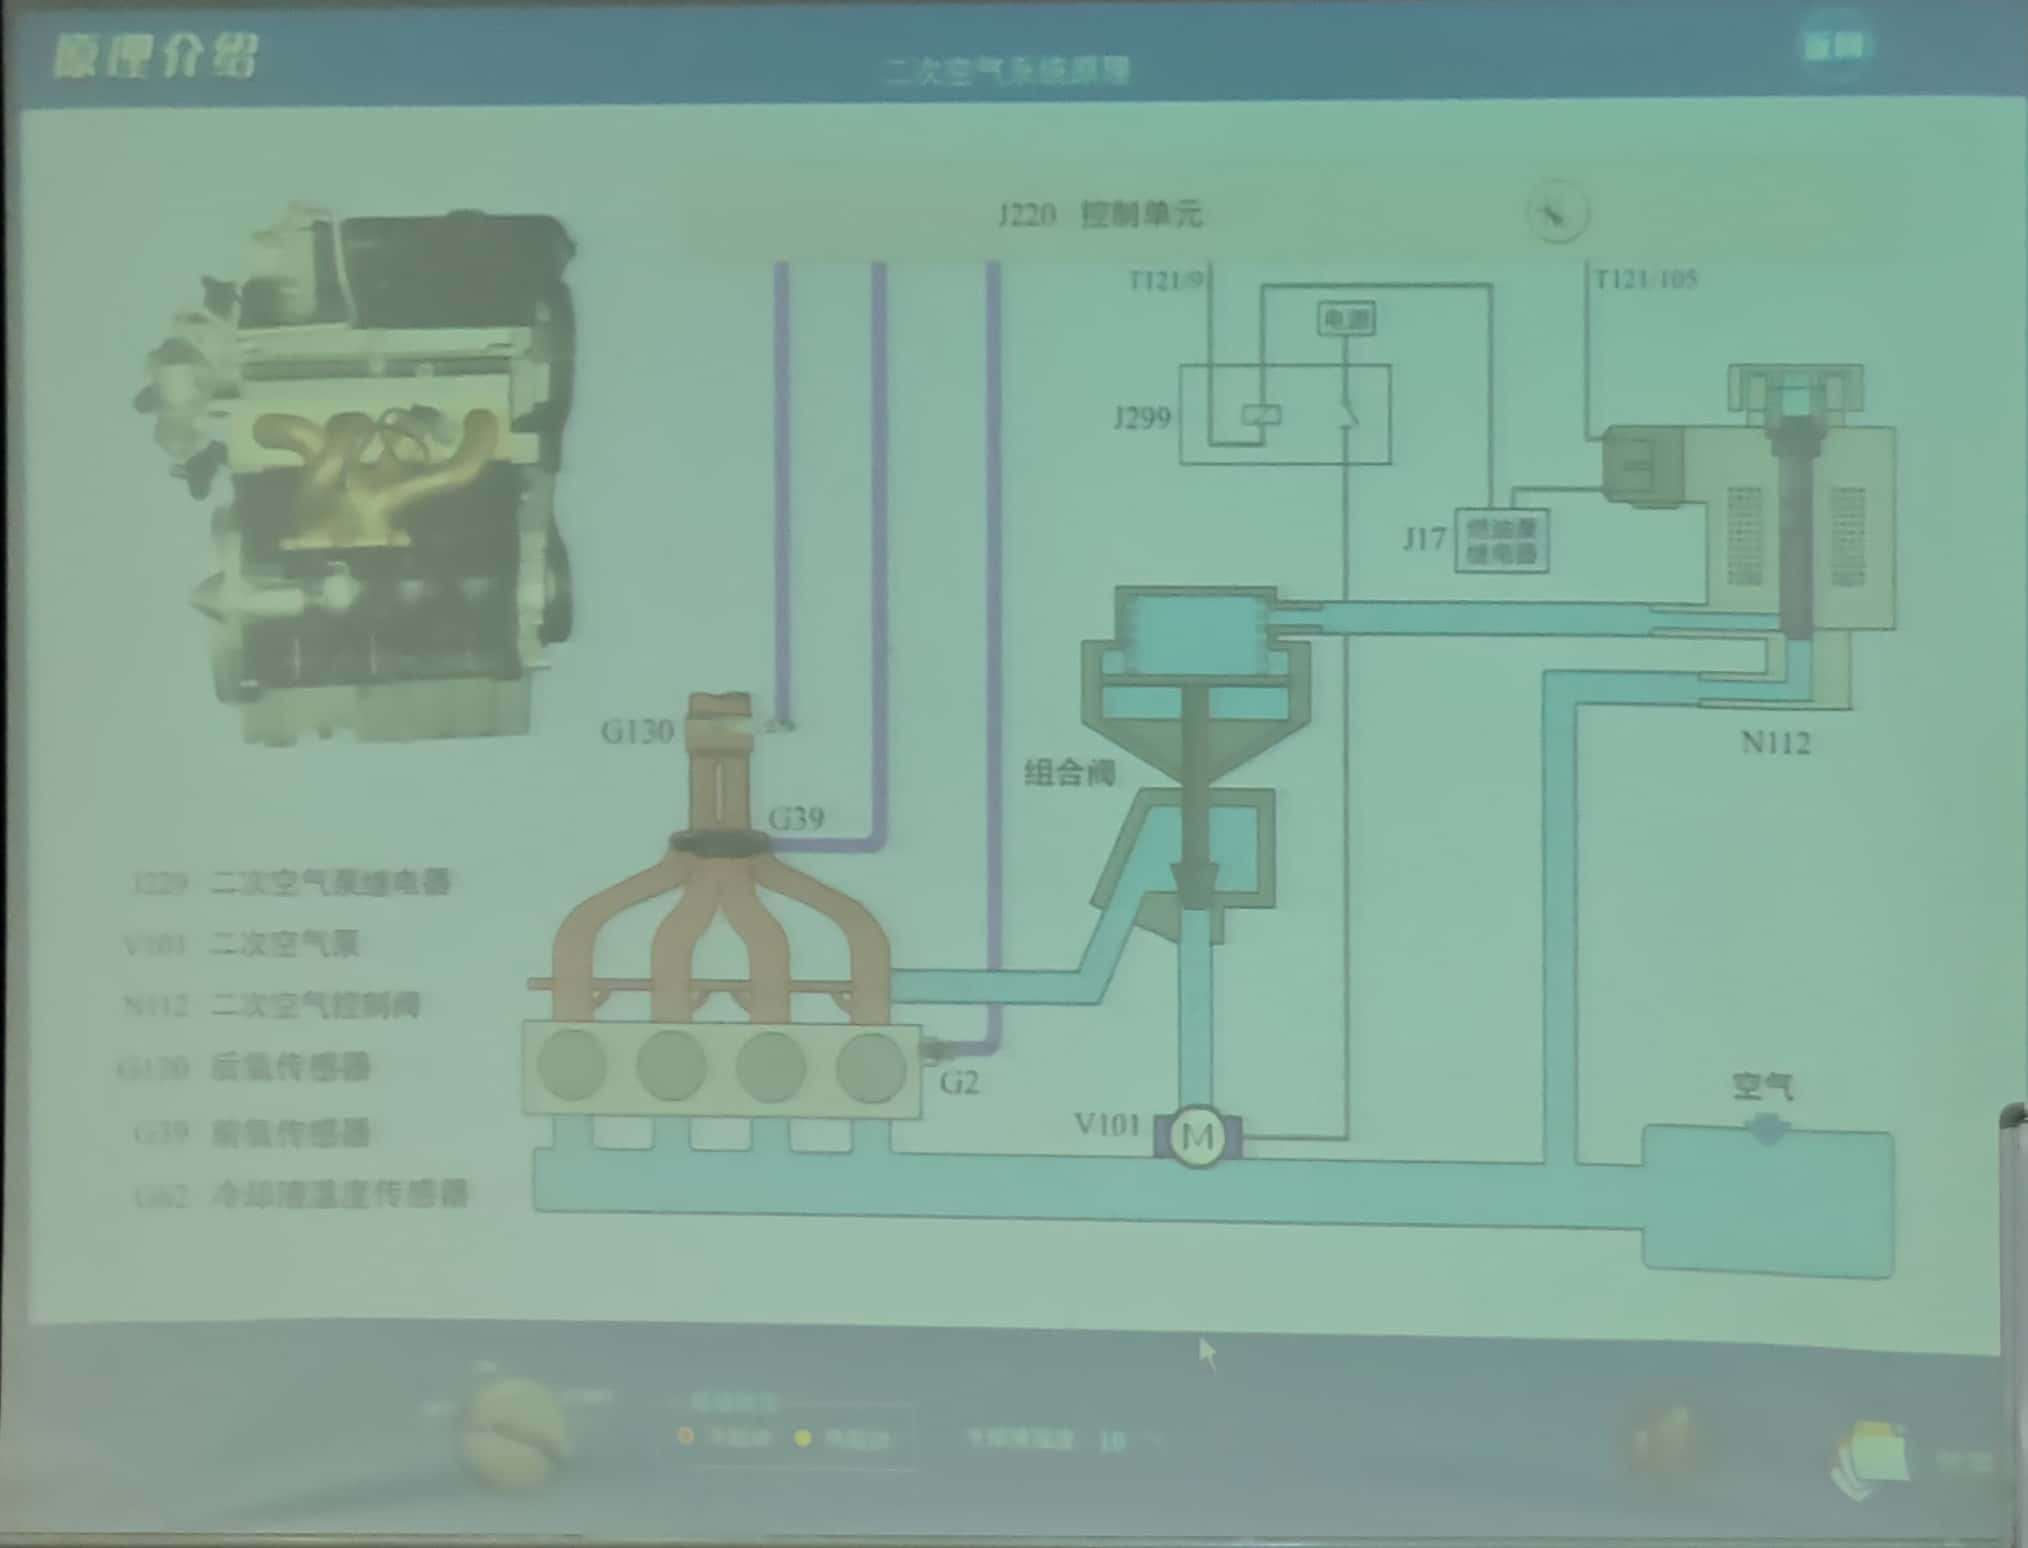
\includegraphics[width=0.3\textwidth]{secondary air}\label{secondary air}}
	\subfigure[排气再循环]{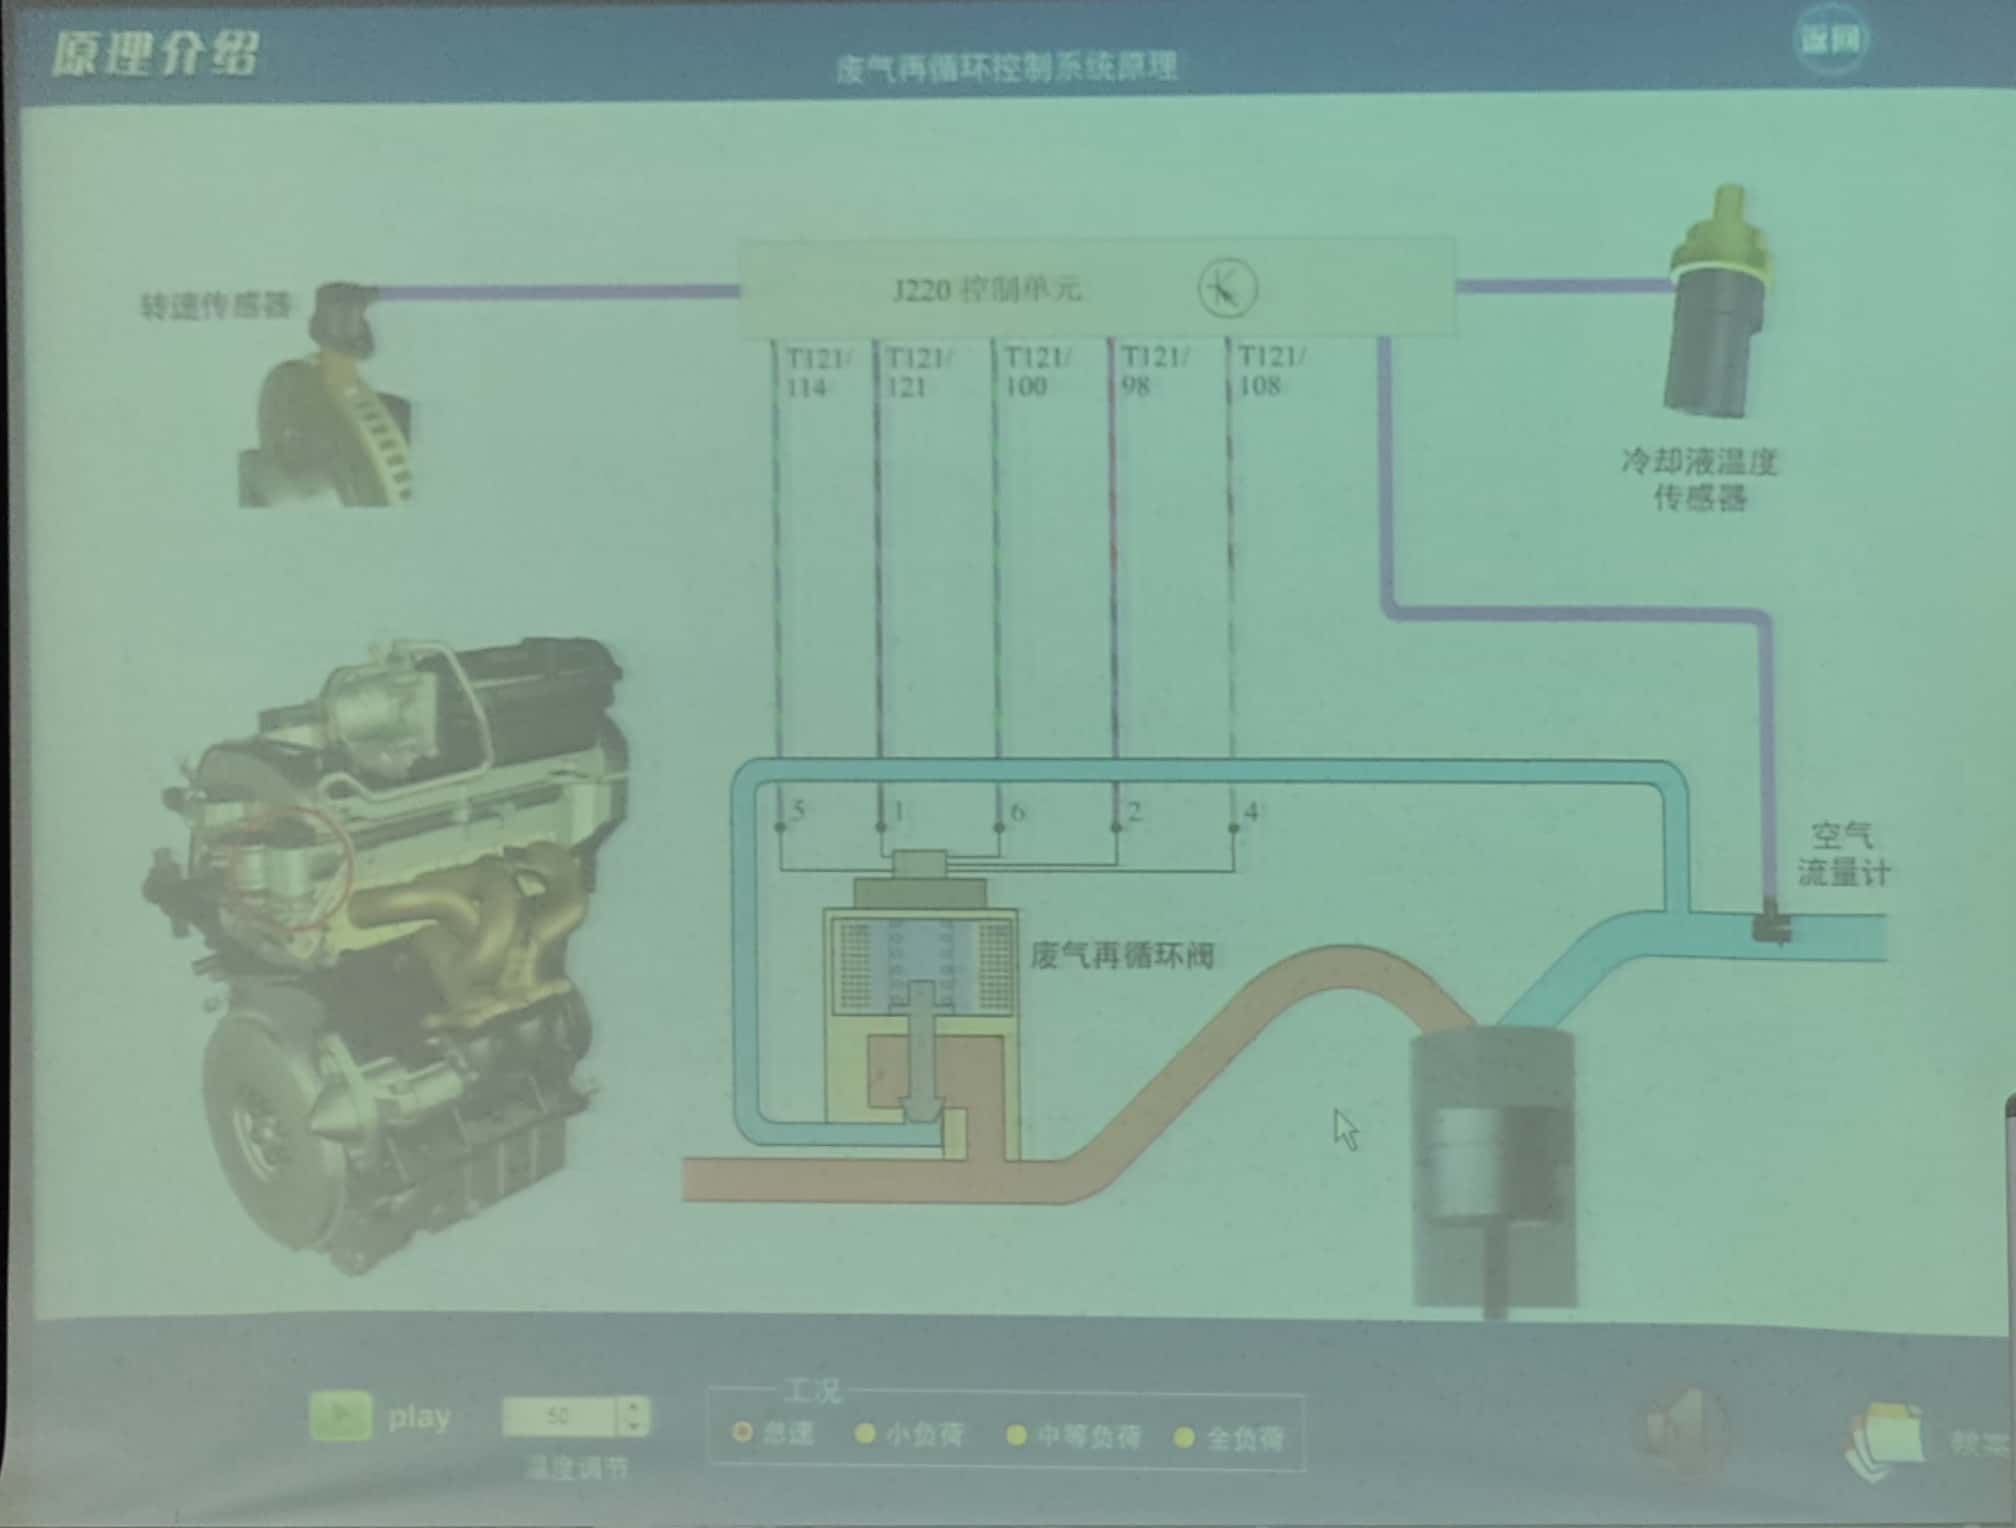
\includegraphics[width=0.3\textwidth]{EGR}\label{EGR}}
	\subfigure[废气涡轮增压]{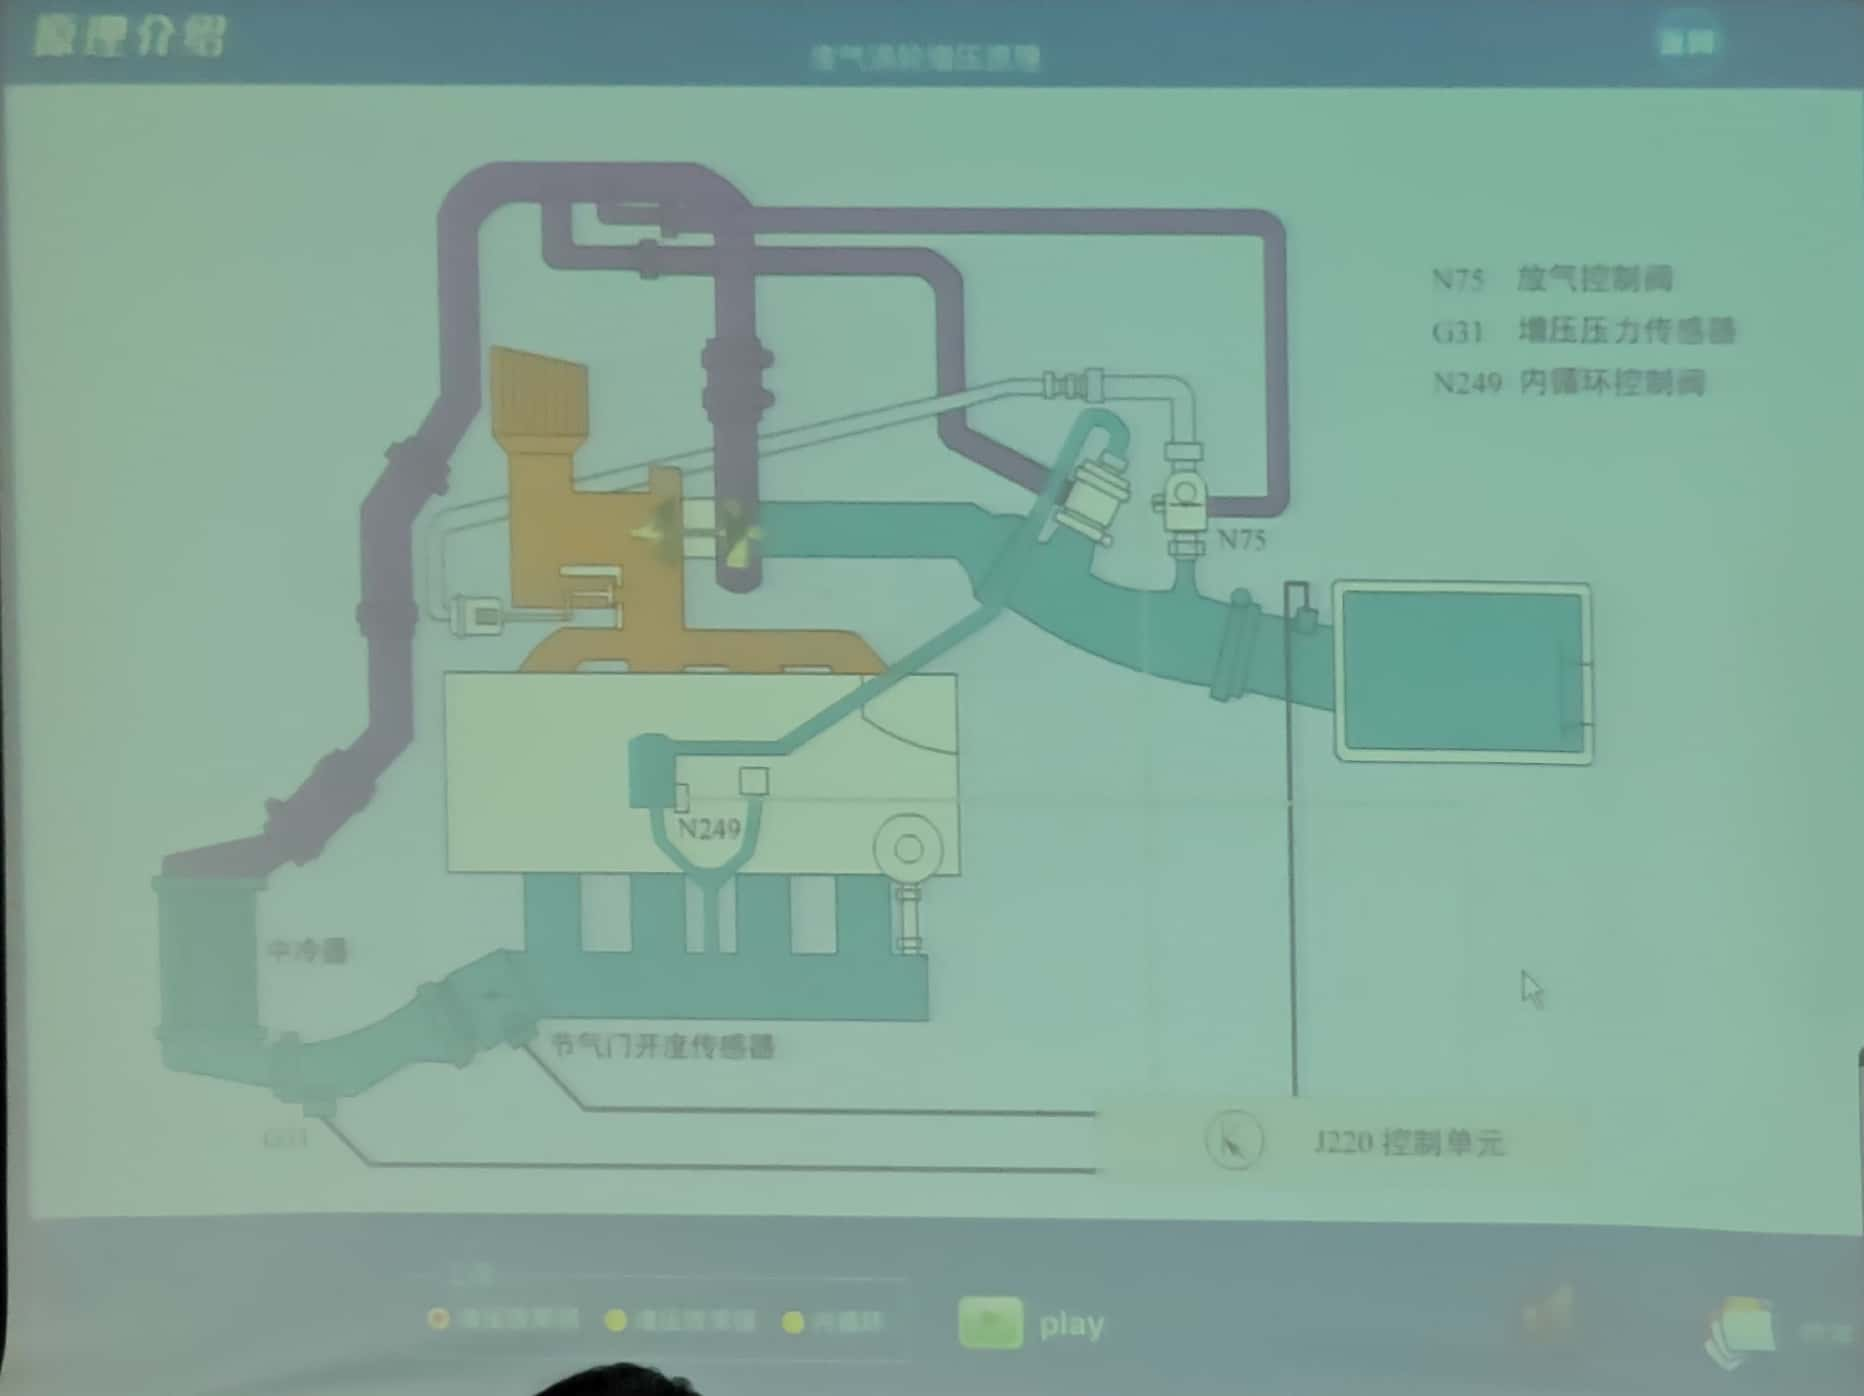
\includegraphics[width=0.3\textwidth]{turbocharging}\label{turbocharging}}
	\caption{发动机的控制系统中的部分执行器}
	\label{actuators}
\end{figure}

\subsection{请简述车身的主要功能及其实现方式。}

汽车车身是驾驶人的工作场所,也是装载乘客和货物的场所。

车身为驾驶员提供良好的操作条件,为乘员提供舒适的乘坐条件,并保证完好无损地运载货物且装卸方便。车身四周装有车窗,车身内外配备后视镜,部分新款汽车在车身周围还安装了多组传感器,驾驶员能清晰地感知车周环境。车内有仪表板,座椅、方向盘、后视镜等附件的位置可调,方便驾驶员掌握车辆情况。对乘员来说,发动机舱盖上有隔音棉(\cref{sound insulation cotton}),车门和车顶中空除方便车窗、天窗开闭外也可提升隔音、隔热效果,炽热的排气管与车身底部间覆盖隔热材料(\cref{insulation}),可开合的门四周覆盖胶条密封以隔音、防水,舒适的座椅起部分隔振功能,这些措施都让乘员与外界较恶劣的环境隔绝,提升舒适性。车身上开门位置合理,乘员能方便上下车,货物能方便装卸。对于货车来说车身上设有货物固定装置,避免运输时货物滑移、倾倒。

\begin{figure}[htbp]
	\centering
	\begin{minipage}[b]{0.7\textwidth}
		\centering
		
\includegraphics[width=\textwidth]{sound insulation cotton}
		\caption{隔音棉}
		\label{sound insulation cotton}
	\end{minipage}
	\begin{minipage}[b]{0.25\textwidth}
		\centering
		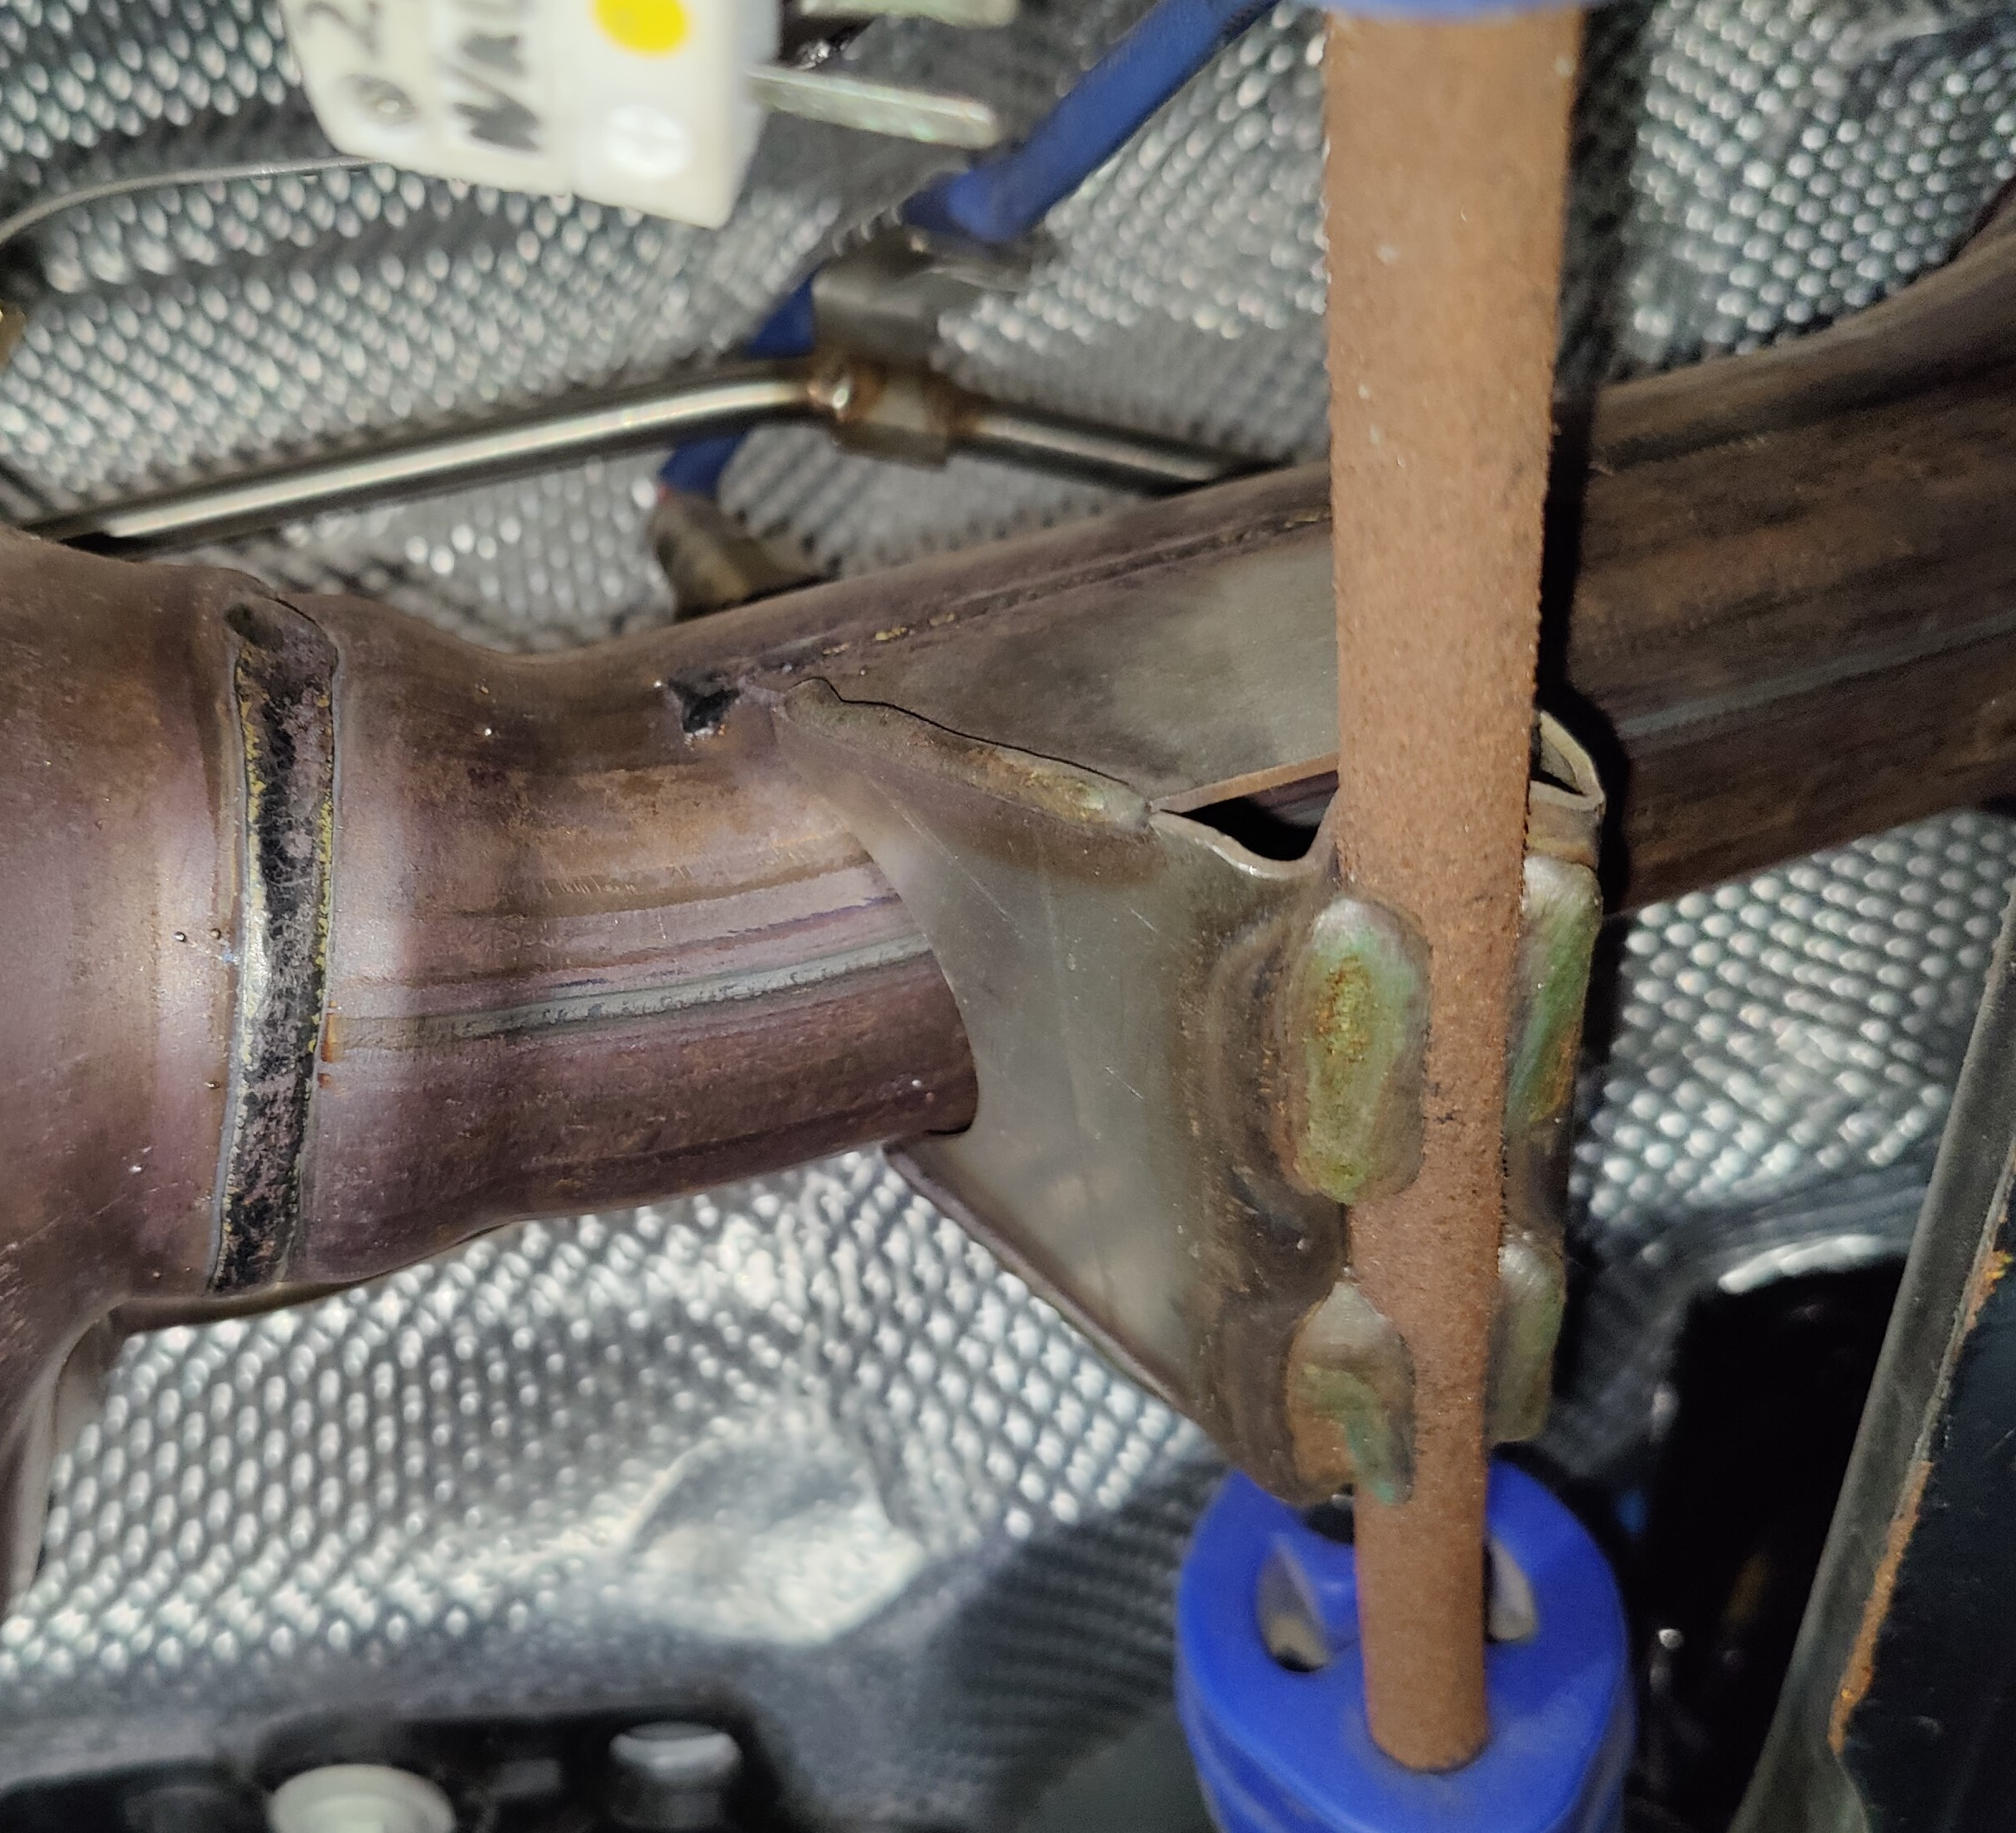
\includegraphics[width=\textwidth]{insulation}
		\caption{隔热材料}
		\label{insulation}
	\end{minipage}
\end{figure}

碰撞安全性是车身结构和设备设计时需要重点考虑的。\cref{BIW}为白车身的一部分,注意到涂有红色油漆的钢梁均由高强钢制成,起防撞梁的作用。保险杠安装梁与车身本体间有缓冲装置,部分高配车型上这里会安装弹性元件和阻尼器,缓和正碰时冲击。车门内部也有高强度的防撞梁,增强侧碰安全性。车上装有多个安全气囊,和安全带一起避免碰撞时乘员重要部位直接与硬物接触,保护乘员。现在对行人保护日趋重视,车身上通过吸能保险杠、软性的引擎盖材料、大灯及附件无锐角等措施保护低速碰撞时行人的安全。

\begin{figure}[htbp]
	\centering
	\begin{minipage}[b]{0.6\textwidth}
		\centering
		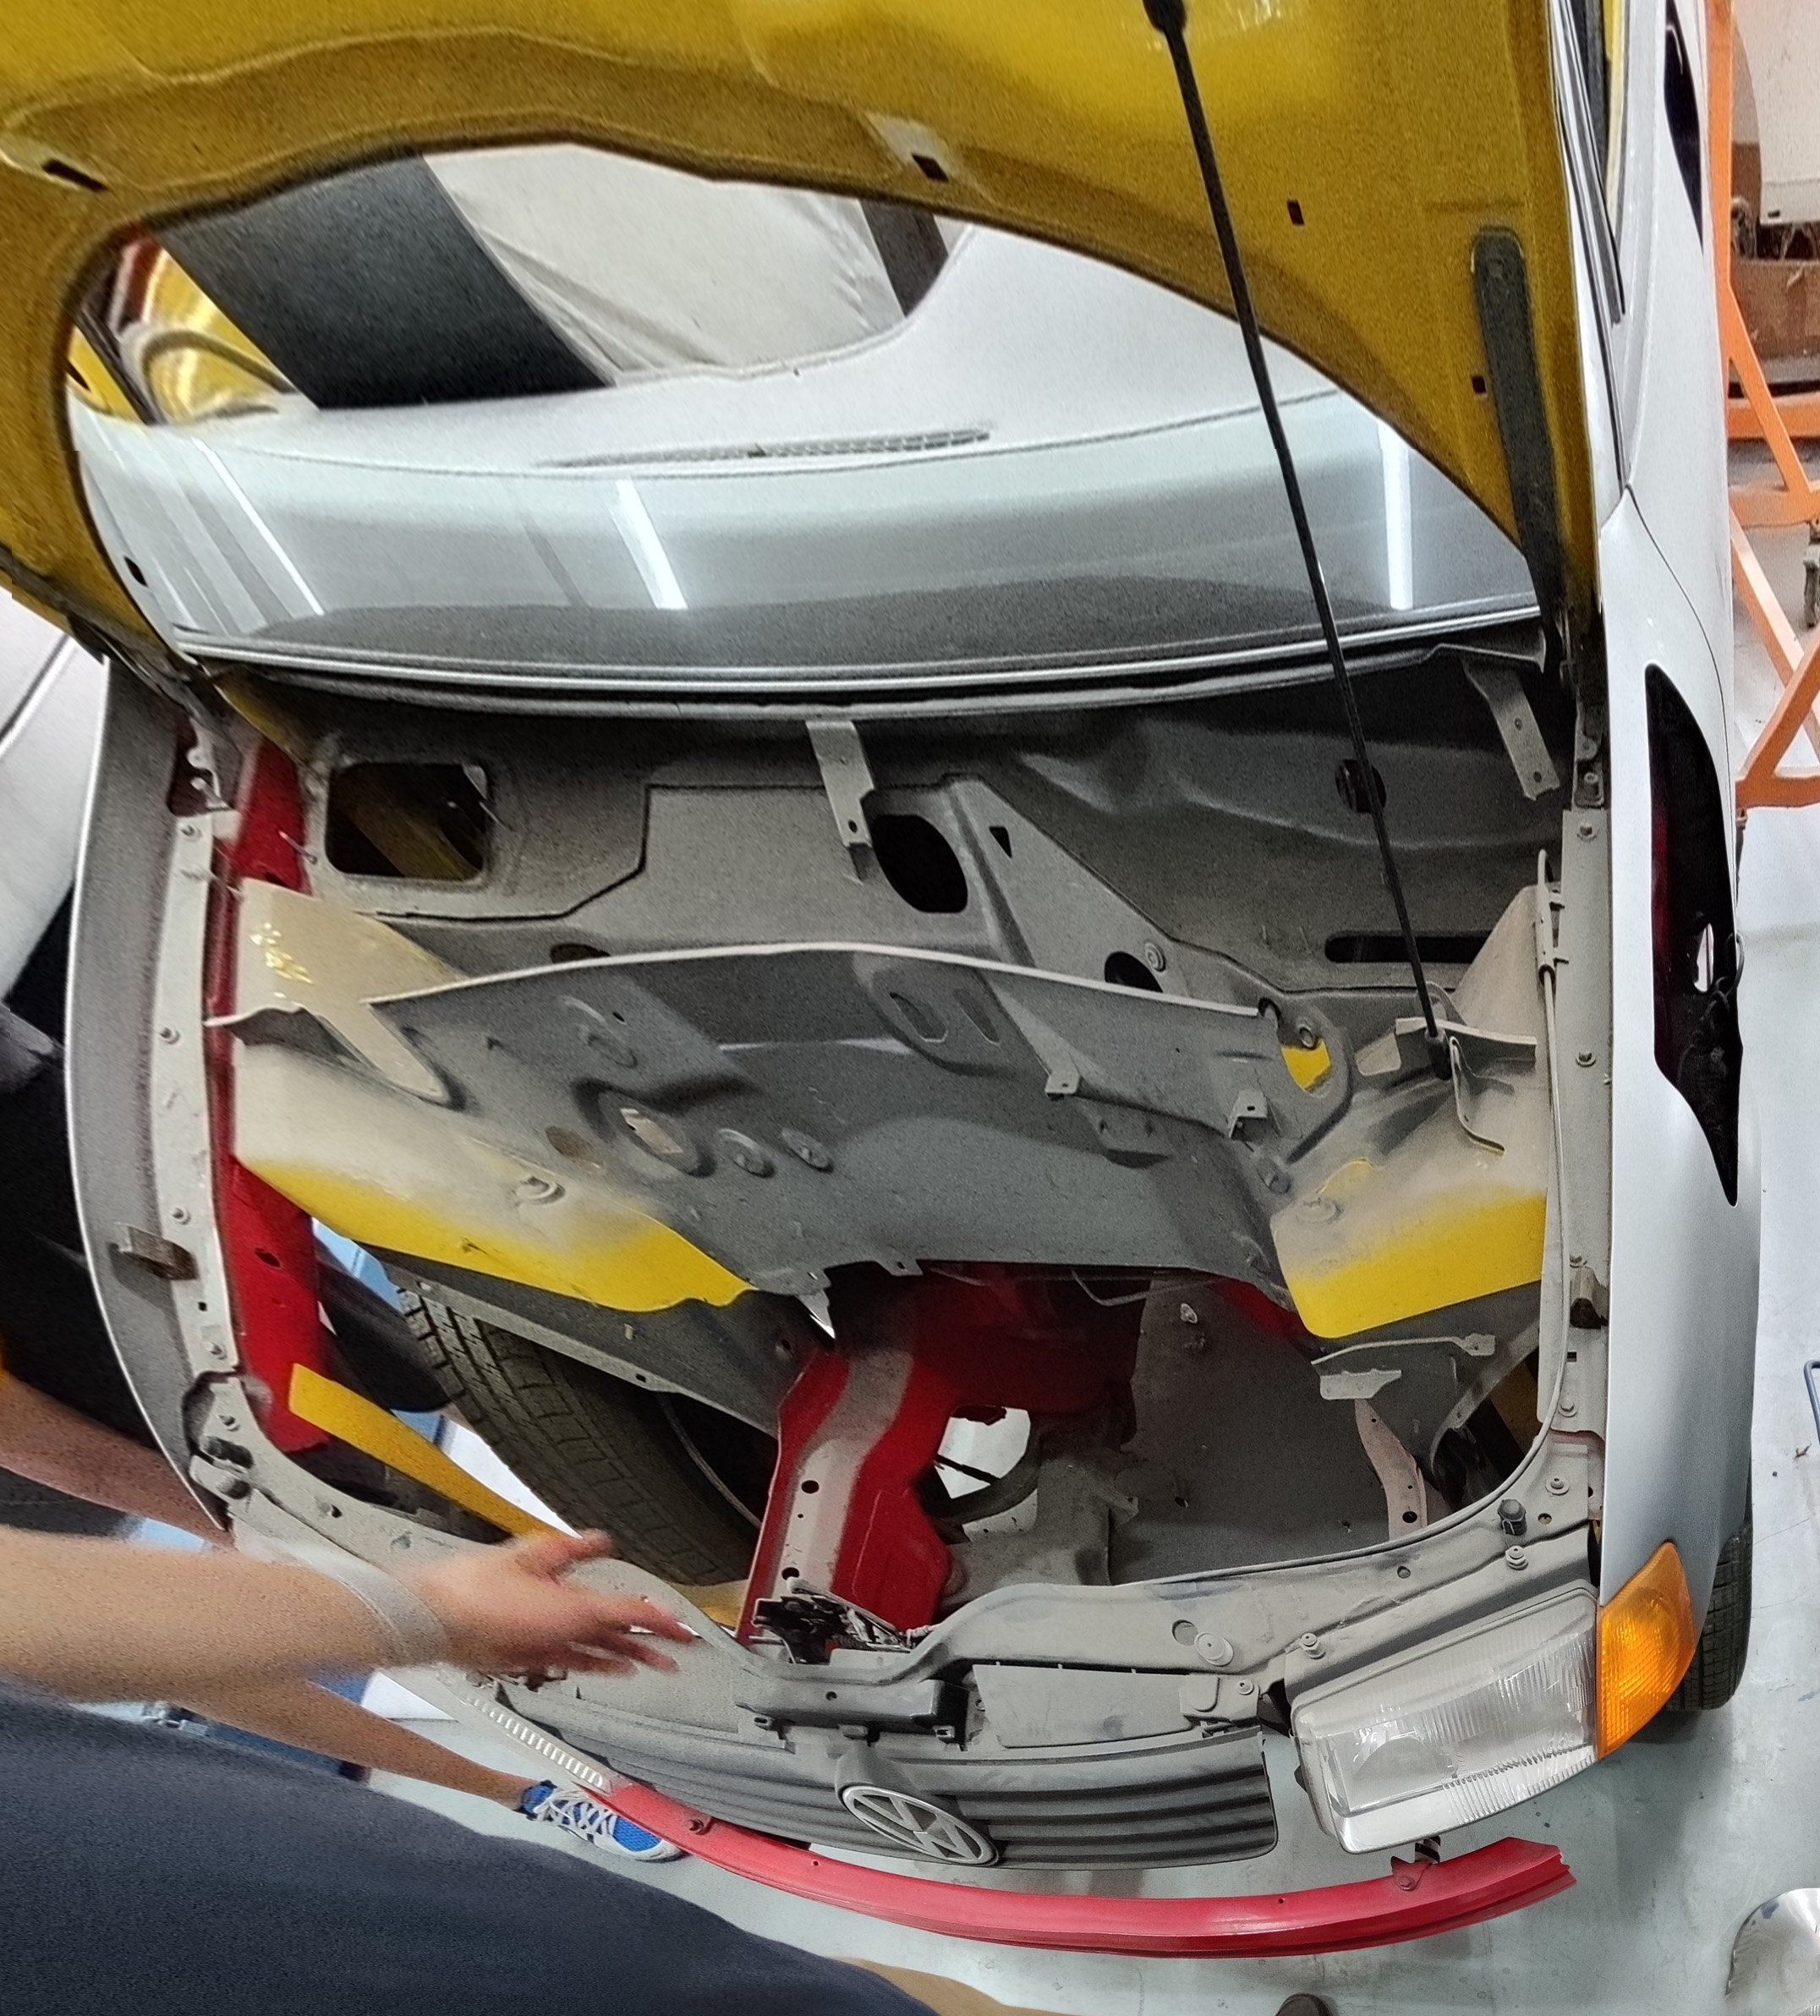
\includegraphics[width=\textwidth]{BIW}
		\caption{白车身}
		\label{BIW}
	\end{minipage}
\end{figure}

车身外形的设计要考虑空气动力学特性,以便汽车行驶时能有效引导周围的气流,提高汽车动力性和行驶稳定性,并改善发动机舱冷却条件和车内通风。注意到展示的领克02上发动机底板已被拆下(\cref{engine compartment bottom}),这能让我们方便地看到油底壳等发动机部件,但在车辆行驶过程中会带来较大的风阻增加,故实际车辆上发动机舱底部有一平板用于引导气流,如\cref{engine compartment with floor}所示,该底板还可兼起保护油底壳免受异物碰撞的作用。对于一般的发动机前置车型,车身头部开有进气孔,还可布置冷排,供发动机进气、冷却。现在的车身越来越向流线型发展,这主要也是出于降阻的考虑。

\begin{figure}[htbp]
	\centering
	\begin{minipage}[b]{0.4\textwidth}
		\centering
		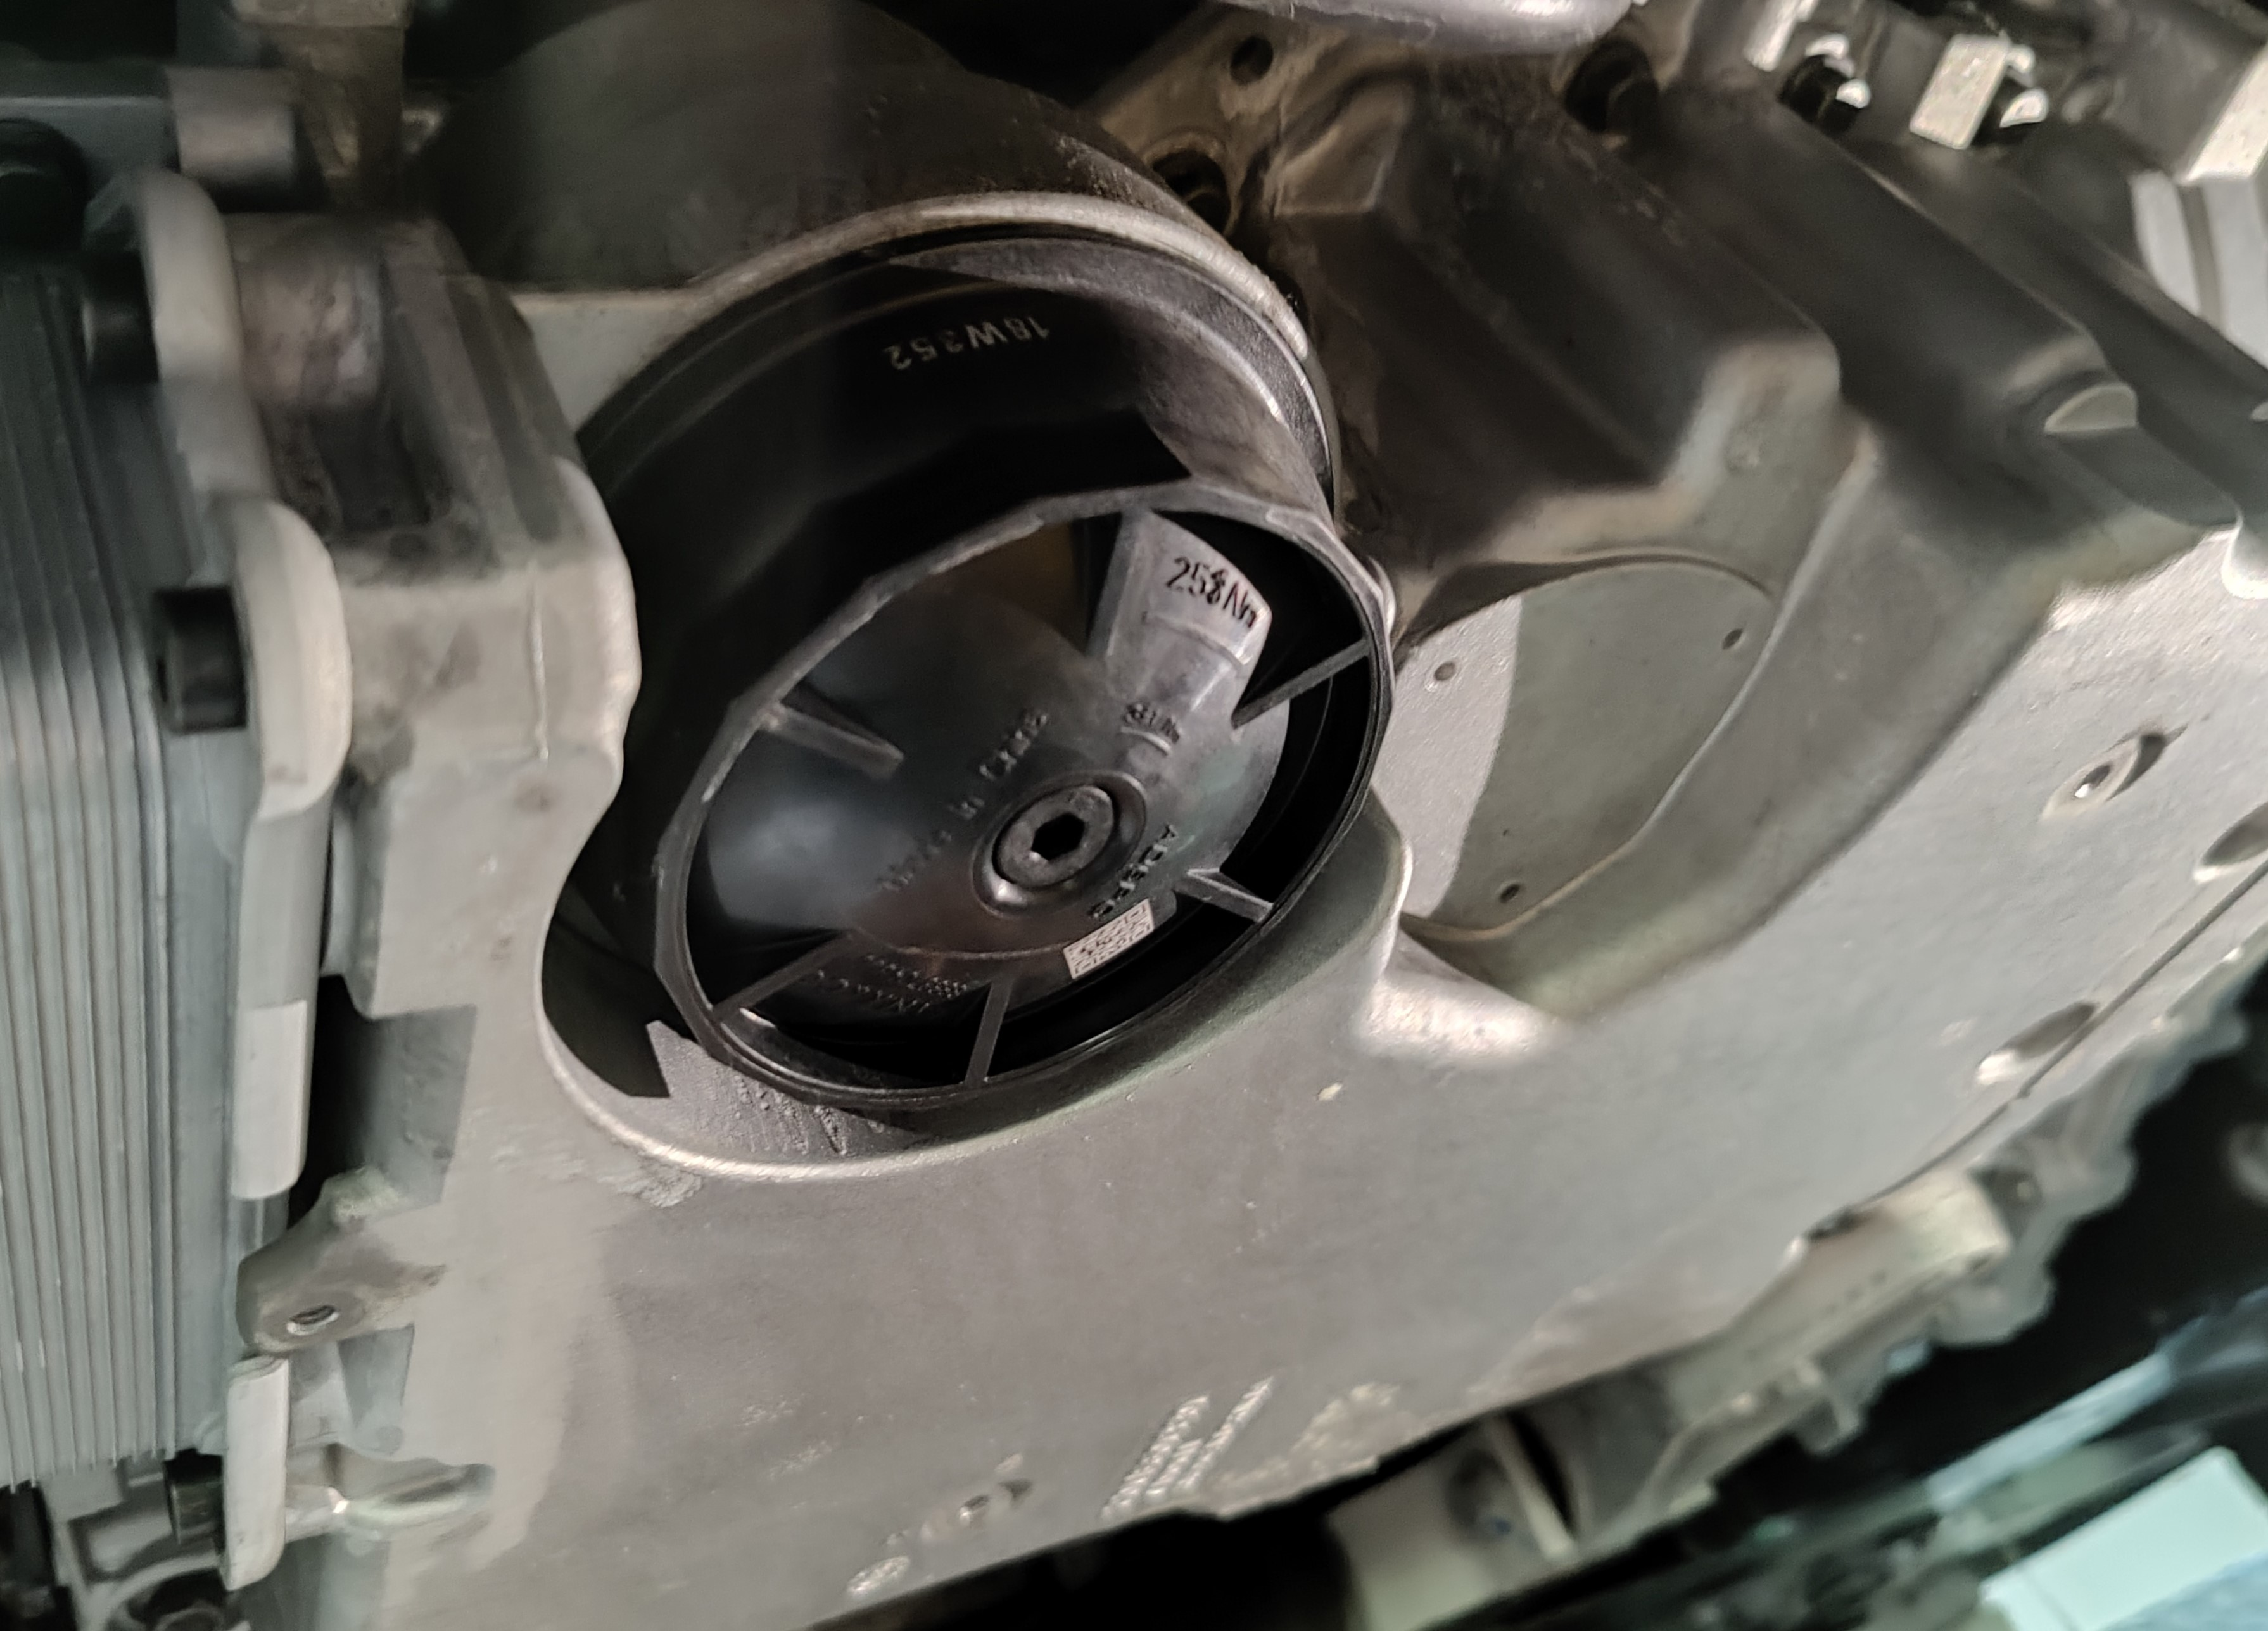
\includegraphics[width=\textwidth]{engine compartment bottom}
		\caption{发动机舱底部}
		\label{engine compartment bottom}
	\end{minipage}
	\begin{minipage}[b]{0.5\textwidth}
		\centering
		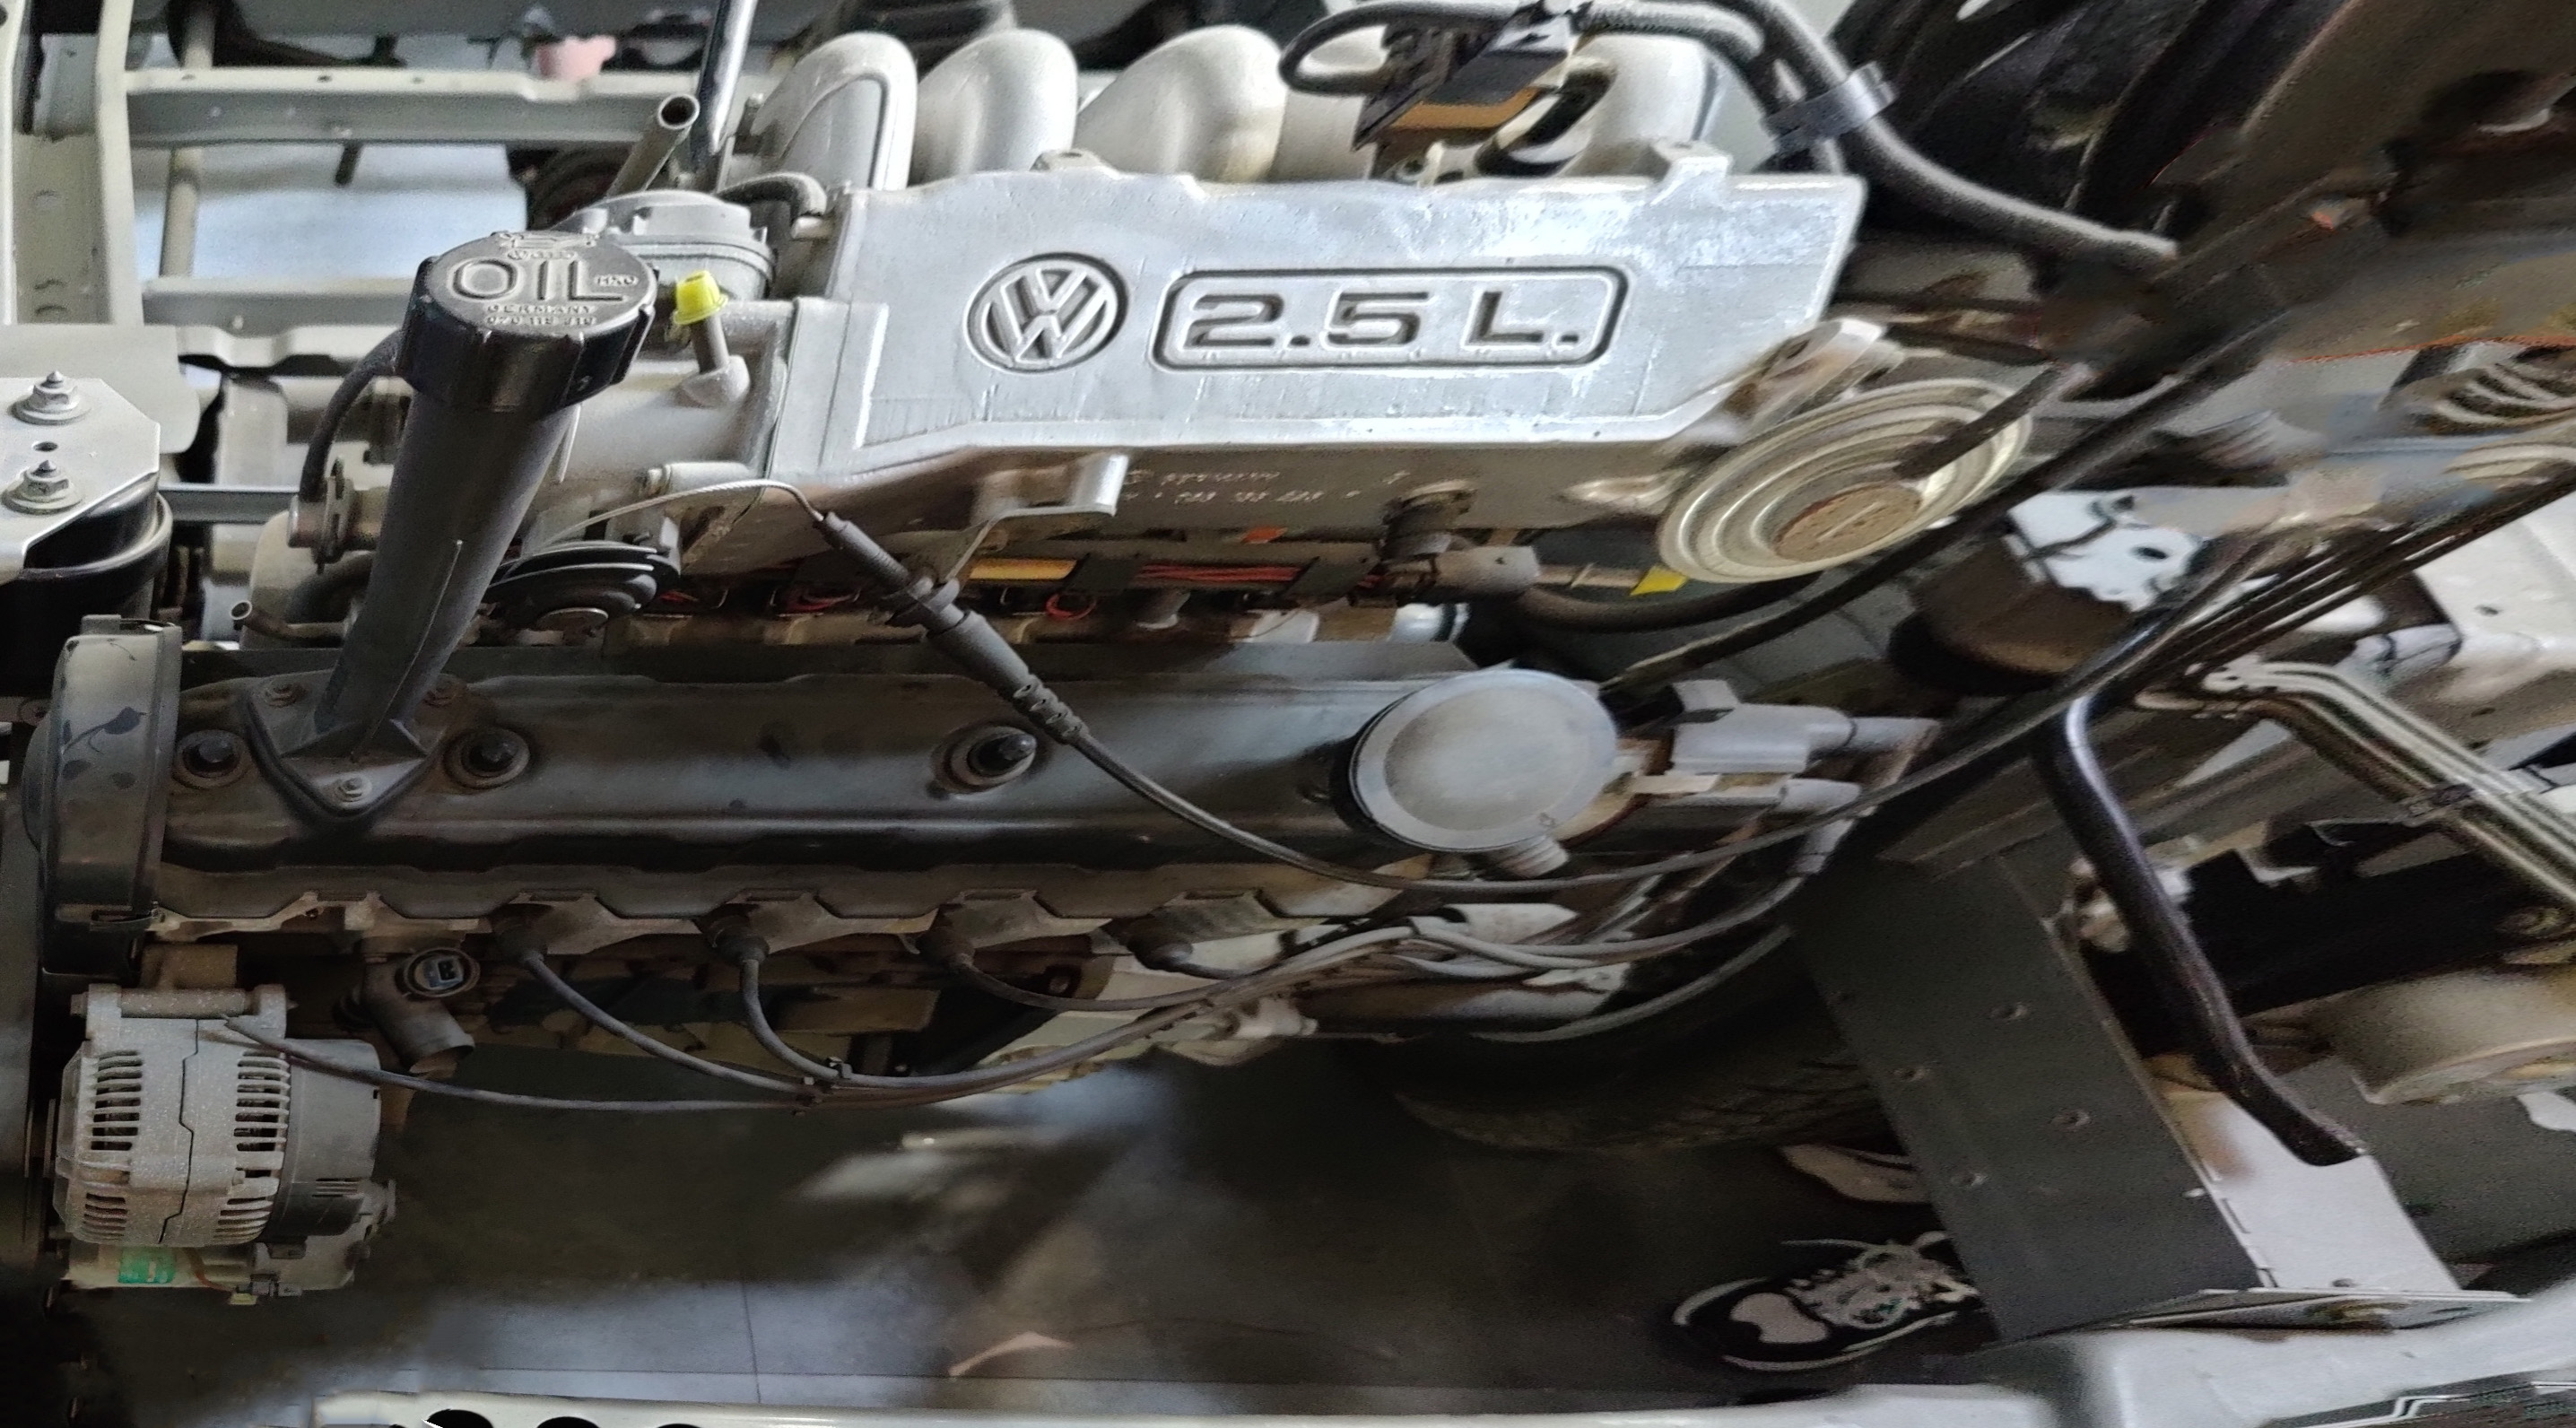
\includegraphics[width=\textwidth]{engine compartment with floor}
		\caption{带底板的发动机舱}
		\label{engine compartment with floor}
	\end{minipage}
\end{figure}

车身是一件精致的艺术品,以其优雅的雕塑形体、装饰件和内部覆饰以及悦目的色彩使人获得美感享受,反映时代的风貌、民族的传统和独特的企业形象。每辆车前后都有车标,但很多时候我们看清车标前就已能知道车辆的品牌。宝马的前脸、普桑的尾灯、法拉利的赛车红、劳斯莱斯的欢庆女神,凡此种种都已成为一款车家族性的标志。

现在乘用车常用承载式车身,车身还得承担起车架的功能,包括支撑连接汽车的各零部件、并承受来自车内外的各种载荷。车身既要承力,又要尽可能地轻量化,对现代的车身设计提出了更高要求。

% \subsection{请简述自动变速箱的换挡离合器和换挡制动器的主要组成部分及其工作原理。}
% \subsection{请简述增压发动机进气系统的主要组成部分及其功能。}
\clearpage

\section{变速箱部分}
\subsection{手动变速器一般有哪些档位? 试述各档的动力传递路线。}

\label{subsection:2.1}

手动变速器一般为普通齿轮式变速器,也称轴线固定式变速器,它按照变速器传动齿轮轴的数目,可分为两轴式变速器和三轴式变速器(也称中间轴式变速器)。目前,轿车和轻、中型货车变速器通常有\numrange[range-phrase = $\,\sim\,$]{3}{5}个前进挡和一个倒挡,重型货车用组合式变速器中会有更多的挡位。三轴式变速器有真正的直接挡,部分变速器还设传动比小于1的超速挡,供良好路面行驶用。一般我们说的变速器挡位数,都指的是前进挡位数。

\cref{two-shaft manual transmission}为一用于纵置发动机的两轴式变速器(注意到图上注为2/3挡同步器的实为3/4挡同步器),和我们在拆装实践中用的那一型结构十分相似,动力传动路线也已在图中标出。对于该变速器:\\
1挡的动力传递路线为:输入轴(包括其上的1挡齿轮)$\rightarrow$输出轴1挡齿轮$\rightarrow$接合齿圈$\rightarrow$接合套$\rightarrow$花键毂$\rightarrow$输出轴;\\
2挡的动力传递路线为:输入轴(包括其上的2挡齿轮)$\rightarrow$输出轴2挡齿轮$\rightarrow$接合齿圈$\rightarrow$接合套$\rightarrow$花键毂$\rightarrow$输出轴;\\
3挡的动力传递路线为:输入轴$\rightarrow$花键毂$\rightarrow$接合套$\rightarrow$接合齿圈$\rightarrow$输入轴3挡齿轮$\rightarrow$输出轴3挡齿轮$\rightarrow$输出轴;\\
4挡的动力传递路线为:输入轴$\rightarrow$花键毂$\rightarrow$接合套$\rightarrow$接合齿圈$\rightarrow$输入轴4挡齿轮$\rightarrow$输出轴4挡齿轮$\rightarrow$输出轴;\\
5挡的动力传递路线为:输入轴$\rightarrow$花键毂$\rightarrow$接合套$\rightarrow$接合齿圈$\rightarrow$输入轴5挡齿轮$\rightarrow$输出轴5挡齿轮$\rightarrow$输出轴;\\
倒挡的动力传递路线为:输入轴$\rightarrow$输入轴倒挡齿轮$\rightarrow$倒挡中间齿轮$\rightarrow$输出轴倒挡齿轮$\rightarrow$输出轴。

\begin{figure}[htbp]
	\centering
	\begin{minipage}[b]{\textwidth}
		\centering
		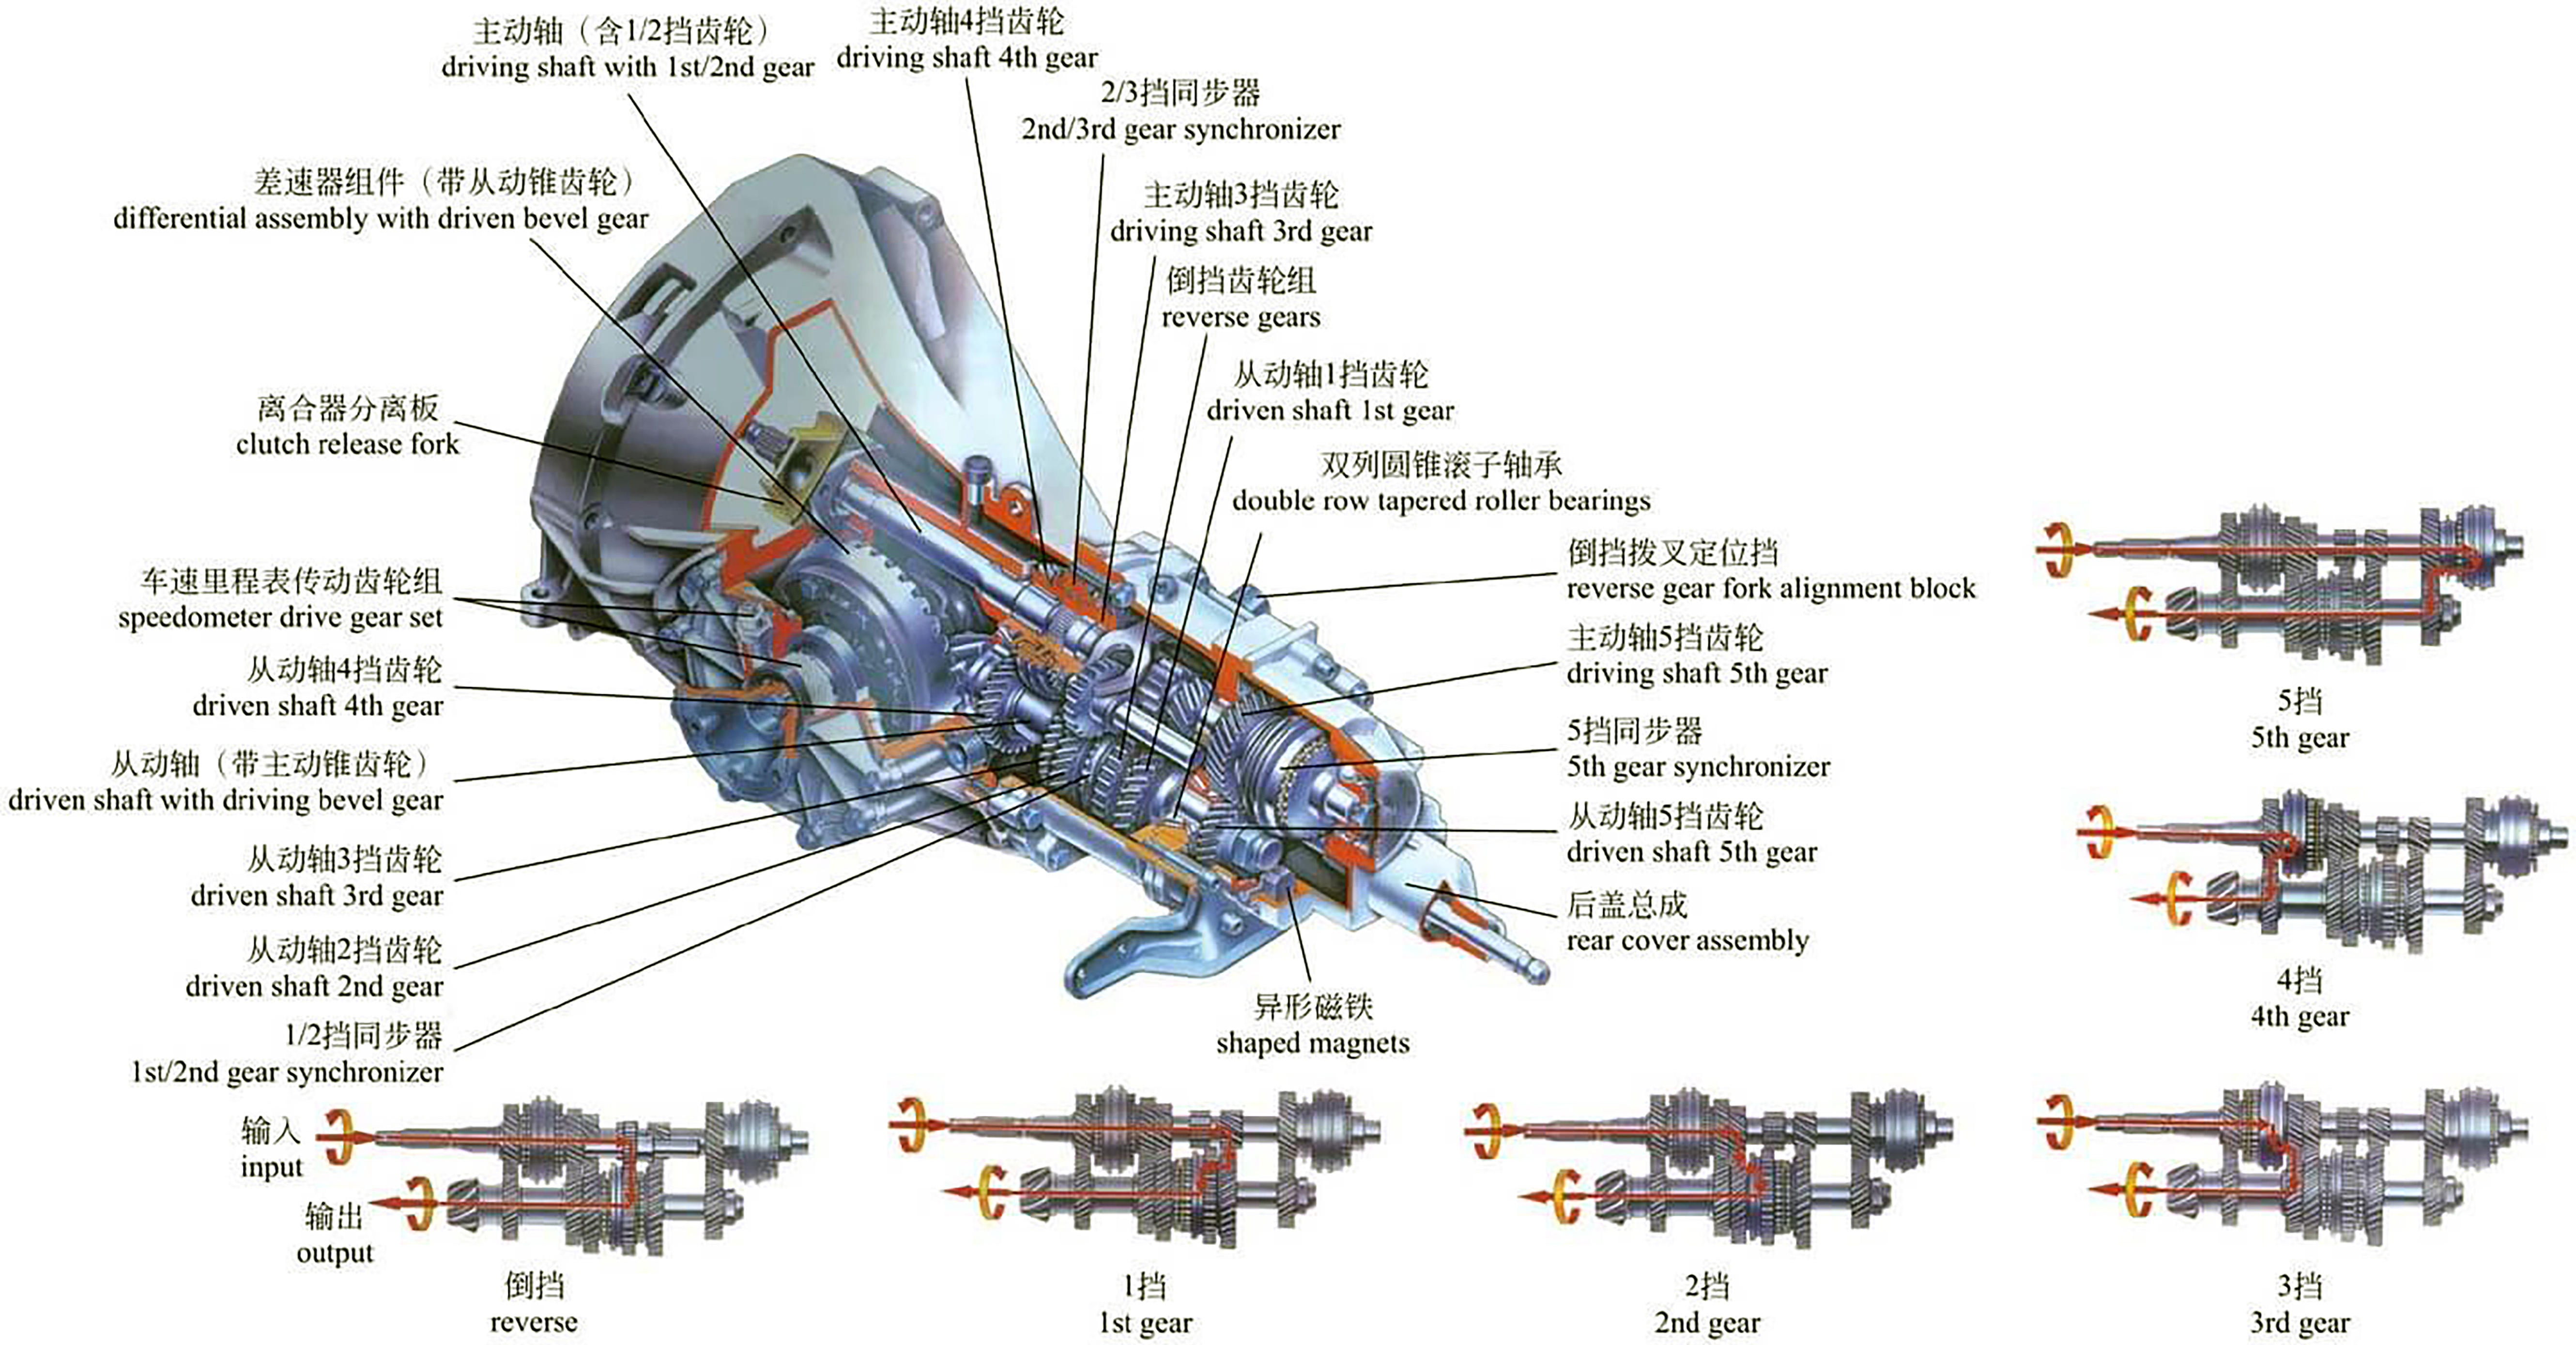
\includegraphics[width=\textwidth]{two-shaft manual transmission}
		\caption{两轴式5挡手动变速器}
		\label{two-shaft manual transmission}
	\end{minipage}
\end{figure}

\cref{three-shaft manual transmission}为课本上提到的一种三轴式变速器,它的特点是具有直接挡。在该变速器中,1、倒挡采用接合套换挡,其余各挡位采用同步器换挡,其中2挡使用锁销式同步器以承受更大载荷,\numrange[range-phrase = $\,\sim\,$]{3}{6}挡使用锁环式同步器。对该变速器:\\
1挡的动力传递路线为:第一轴$\rightarrow$第一轴常啮齿轮$\rightarrow$中间轴常啮齿轮$\rightarrow$中间轴$\rightarrow$中间轴1挡齿轮$\rightarrow$第二轴1挡齿轮$\rightarrow$接合齿圈$\rightarrow$接合套$\rightarrow$花键毂$\rightarrow$第二轴;\\
2挡的动力传递路线为:第一轴$\rightarrow$第一轴常啮齿轮$\rightarrow$中间轴常啮齿轮$\rightarrow$中间轴$\rightarrow$中间轴2挡齿轮$\rightarrow$第二轴2挡齿轮$\rightarrow$接合齿圈$\rightarrow$接合套$\rightarrow$花键毂$\rightarrow$第二轴;\\
3挡的动力传递路线为:第一轴$\rightarrow$第一轴常啮齿轮$\rightarrow$中间轴常啮齿轮$\rightarrow$中间轴$\rightarrow$中间轴3挡齿轮$\rightarrow$第二轴3挡齿轮$\rightarrow$接合齿圈$\rightarrow$接合套$\rightarrow$花键毂$\rightarrow$第二轴;\\
4挡的动力传递路线为:第一轴$\rightarrow$第一轴常啮齿轮$\rightarrow$中间轴常啮齿轮$\rightarrow$中间轴$\rightarrow$中间轴4挡齿轮$\rightarrow$第二轴4挡齿轮$\rightarrow$接合齿圈$\rightarrow$接合套$\rightarrow$花键毂$\rightarrow$第二轴;\\
5挡的动力传递路线为:第一轴$\rightarrow$第一轴常啮齿轮$\rightarrow$中间轴常啮齿轮$\rightarrow$中间轴$\rightarrow$中间轴5挡齿轮$\rightarrow$第二轴5挡齿轮$\rightarrow$接合齿圈$\rightarrow$接合套$\rightarrow$花键毂$\rightarrow$第二轴;\\
6挡(直接挡)的动力传递路线为:第一轴$\rightarrow$第一轴常啮齿轮$\rightarrow$接合齿圈$\rightarrow$接合套$\rightarrow$花键毂$\rightarrow$第二轴;\\
倒挡的动力传递路线为:第一轴$\rightarrow$第一轴常啮齿轮$\rightarrow$中间轴常啮齿轮$\rightarrow$中间轴$\rightarrow$中间轴倒挡齿轮$\rightarrow$倒挡中间齿轮$\rightarrow$第二轴倒挡齿轮$\rightarrow$接合齿圈$\rightarrow$接合套$\rightarrow$花键毂$\rightarrow$第二轴。

\begin{figure}[htbp]
	\centering
	\begin{minipage}[b]{\textwidth}
		\centering
		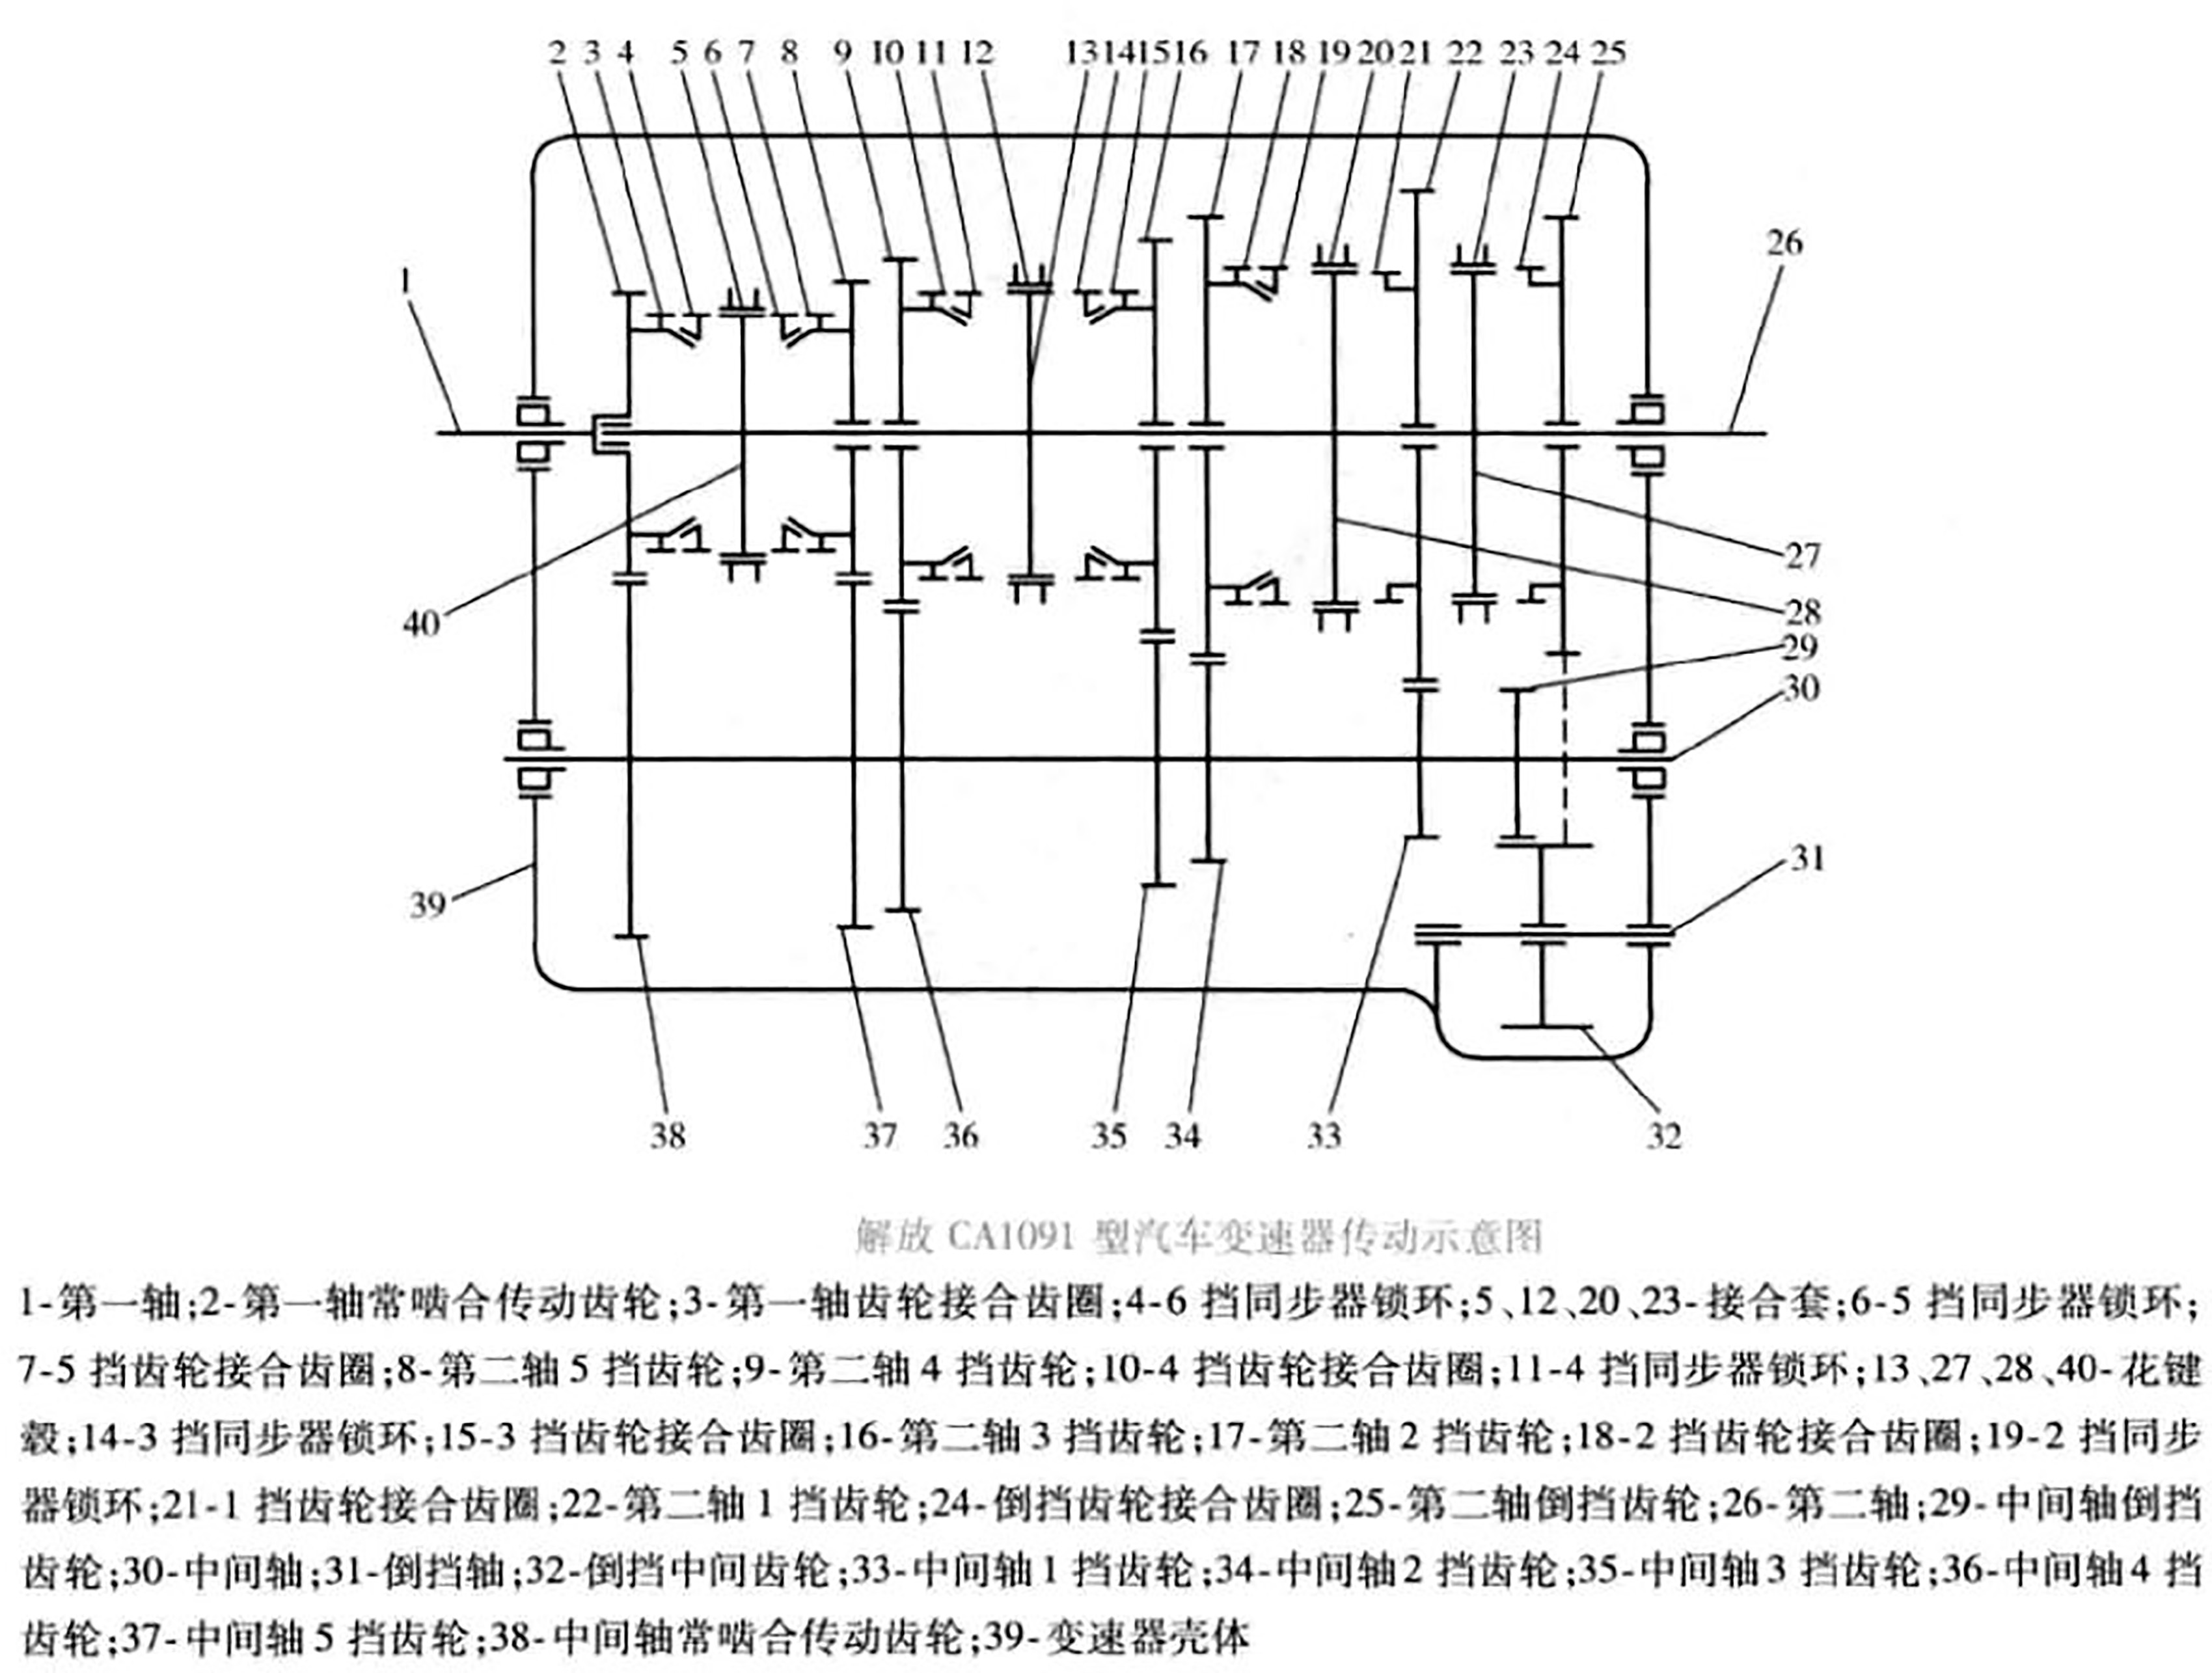
\includegraphics[width=\textwidth]{three-shaft manual transmission}
		\caption{三轴式6挡手动变速器}
		\label{three-shaft manual transmission}
	\end{minipage}
\end{figure}

\subsection{试述自锁与互锁装置的特点和作用。}

为保证变速器在任何情况下都能准确、安全、可靠地工作,其操纵机构必须设置安全装置,包括自锁、互锁和倒挡锁装置。对于六挡变速器,还应设置选挡锁装置。

自锁装置如\cref{self-locking}所示,它的作用主要有三。一是保证操纵变速杆推动拨叉前、后移动距离足够,使得滑动齿轮(或接合套)与相应的齿轮(或接合齿圈)在全齿宽上啮合,提高齿轮的寿命和承载力。二是保证在全齿宽啮合后汽车遇到较大颠簸或其它情况时,滑动齿轮(或接合套)不会自动产生轴向移动造成啮合长度的减小甚至是脱挡。三是为驾驶员提供良好的换挡手感,在钢球滑入凹槽后给驾驶员明显的反馈提示他换挡已到位。

自锁装置由自锁弹簧和自锁钢球组成,每根拨叉轴的表面有与钢球对应的凹槽(\cref{self-locking slots})。当任意一根拨叉轴连同拨叉一起轴向移动到空挡或某一工作挡位时,必有一个凹槽正对钢球,于是钢球被弹簧压嵌入该凹槽内,拨叉轴的轴向位置即被固定,从而拨叉连同滑动齿轮(或接合套)也被固定在空挡或一工作挡位上。当需要换挡时,驾驶员必须通过变速杆对拨叉和拨叉轴施加一定的轴力,这个力又在凹槽与拨叉轴接触的侧面上产生一克服弹簧弹力的纵向分力,将自锁钢球压回孔中,拨叉轴方可轴向移动。拨叉轴表面相邻自锁凹槽间的距离就等于使得在全齿宽上啮合或完全退出啮合所需的拨叉及拨叉轴的轴向移动距离。

注意到,该型变速器的1、2挡拨叉和3、4挡拨叉上均有三个自锁凹槽(\cref{self-locking slots}),中间的一个凹槽较浅,对应空挡,两边的凹槽较深,对应工作挡位。空挡的自锁凹槽较浅的原因可能是在空挡时与拨叉轴连接的滑动齿轮(或接合套)不参与动力传递,可能引起跳挡的干扰力小,且若某个拨叉轴已挂入工作挡位,其它拨叉轴的空挡位置即被互锁保证而无需过强的自锁。略感意外的是,5、倒挡拨叉轴上仅有两自锁凹槽,其中一个较浅,推测为空挡自锁,另一较深的应为5挡自锁。相信倒挡拨叉上有专供倒挡使用的自锁装置,不必在拨叉轴上实现倒挡自锁。

\begin{figure}[htbp]
	\centering
	\begin{minipage}[b]{0.6\textwidth}
		\centering
		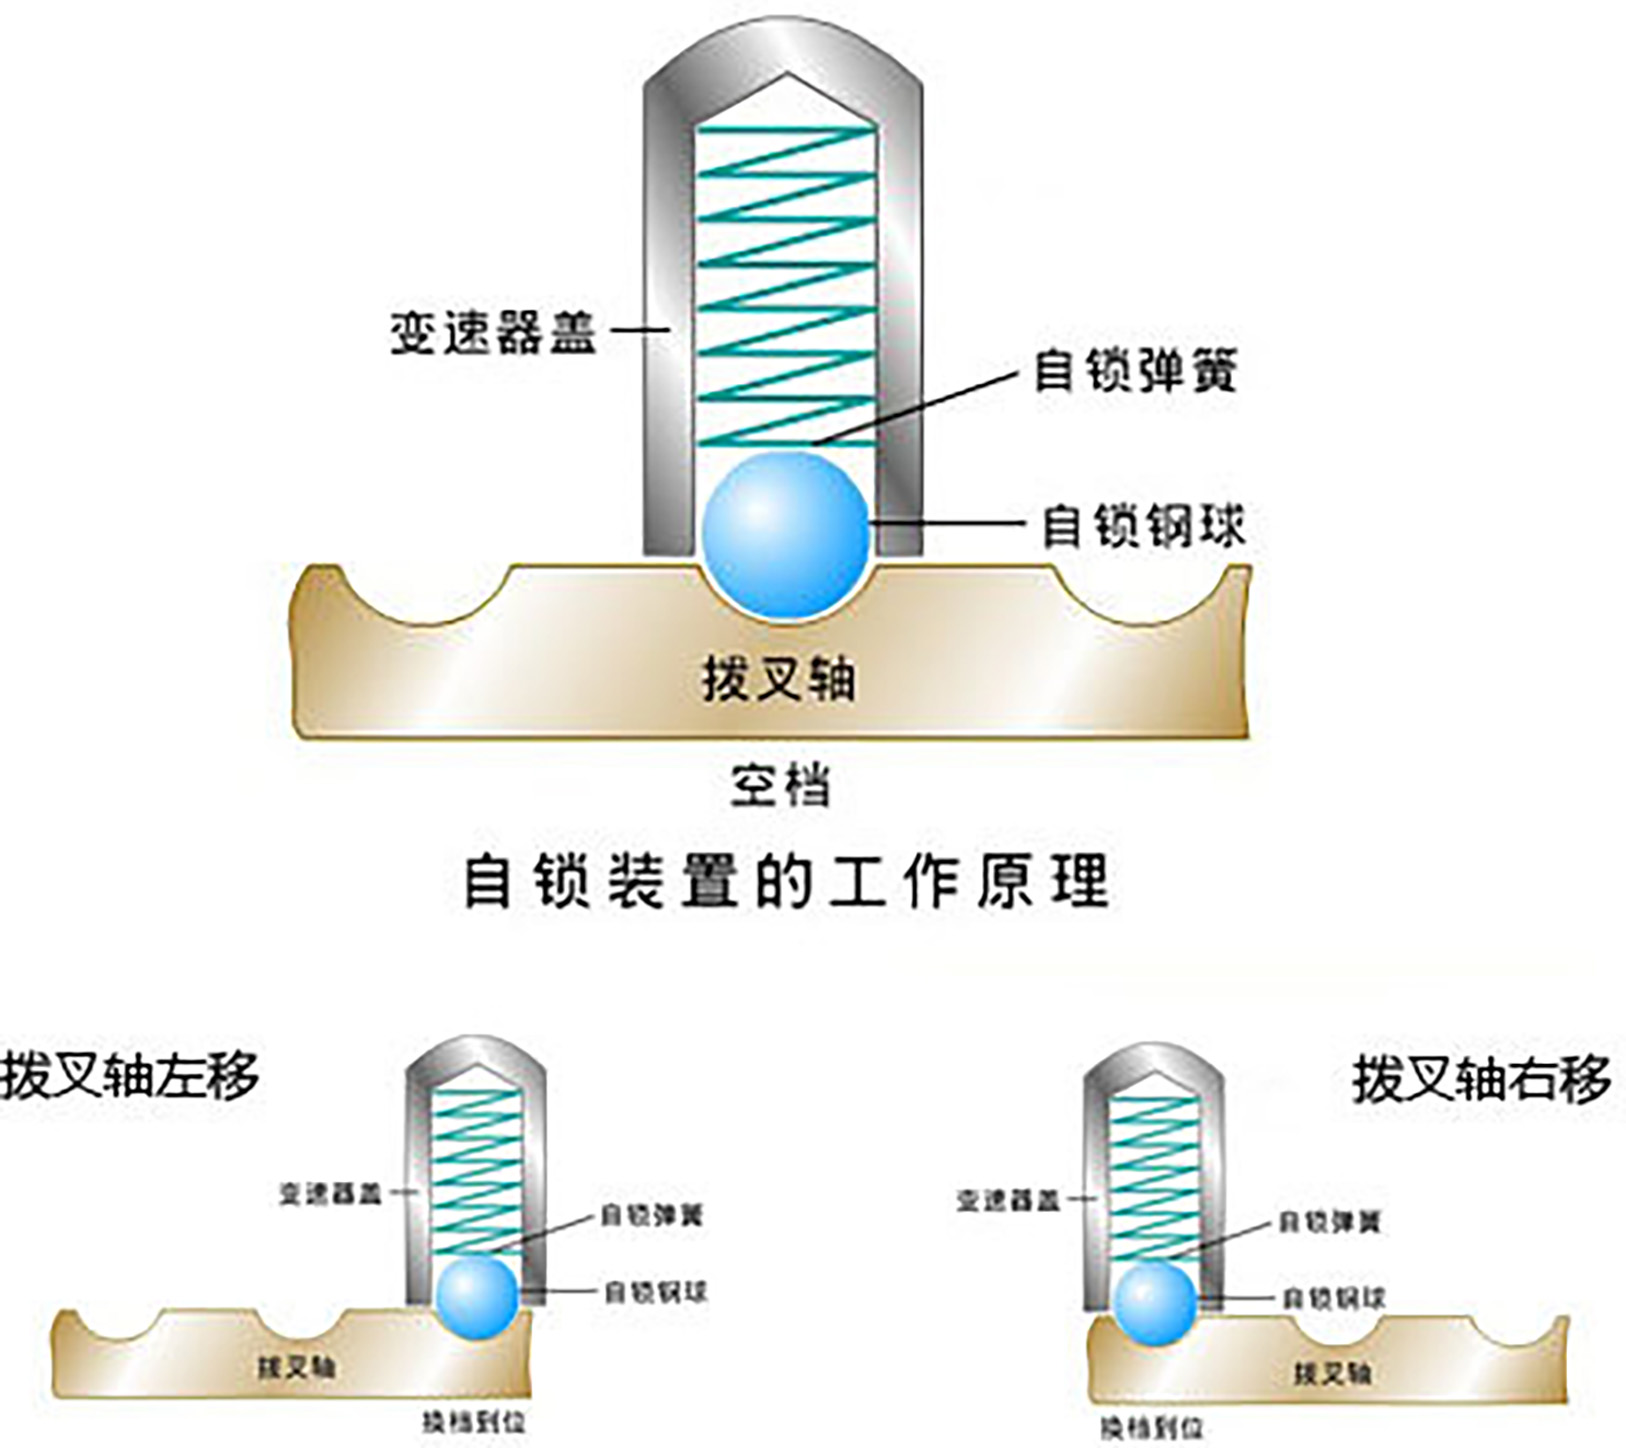
\includegraphics[width=\textwidth]{self-locking}
		\caption{自锁装置示意图}
		\label{self-locking}
	\end{minipage}
	\centering
	\begin{minipage}[b]{0.35\textwidth}
		\centering
		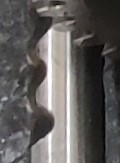
\includegraphics[width=\textwidth]{self-locking slots}
		\caption{自锁凹槽}
		\label{self-locking slots}
	\end{minipage}
	\begin{minipage}[b]{0.5\textwidth}
		\centering
		
\includegraphics[width=\textwidth]{self-locking slots 5R}
		\caption{5、倒挡拨叉轴上的自锁凹槽}
		\label{self-locking slots 5R}
	\end{minipage}
\end{figure}

互锁装置(\cref{interlocking})的作用就是防止变速器同时换入两个挡位。若变速杆能同时推动两个拨叉,则可同时换入两个挡位,但不同挡位的传动比不同,这样就会造成齿轮间的机械干涉,变速器被卡死,此时若传递的动力不消失,会使传动路线中最薄弱处被破坏,产生严重后果。

互锁装置由互锁钢球和互锁销组成,每根拨叉轴朝向互锁钢球的侧表面上均铣出一个深度相等的凹槽,任一拨叉轴处于空挡位置时其侧面凹槽都恰对准互锁钢球。两互锁钢球直径之和等于相邻两轴表面间距离加一凹槽深度。中间拨叉轴上两互锁凹槽间有一孔将二者连同,孔中置有互锁销,销的长度等于拨叉轴的直径减去一凹槽深。当变速器处于空挡时,互锁凹槽、互锁钢球和互锁销都在同一直线上。当移动中间那根拨叉轴时,轴两侧的内互锁钢球被从凹槽中挤出,推动外互锁钢球分别嵌入外侧两根拨叉轴侧面的互锁凹槽中,将两轴锁止在空挡位置。如此时欲像\cref{interlocking}中右侧子图所示那样移动1、2挡拨叉轴,则须先将中间的3、4挡拨叉轴退回空挡位置,再移动1、2挡拨叉轴,互锁钢球便被从1、2挡拨叉轴上的互锁凹槽挤出,推动互锁销和其它互锁钢球将剩余两拨叉轴锁止于空挡。\cref{interlocking}中推动倒挡拨叉轴的过程也类似。可见,互锁装置结构的设计使得驾驶员用变速杆推动某一拨叉轴时能自动锁止其它所有拨叉轴。

在我们的拆装实践中,事实上互锁销和互锁钢球都已被提前取出,我们只能看到定位互锁钢球的凹槽和通互锁销的小孔。减速器中互锁装置和自锁装置做在一起,都位于拨叉轴的安装孔上。自锁弹簧和自锁钢球组成一部件,拨叉轴被取出后仍能保持在变速器盖中而不脱出;但互锁销和互锁钢球都是分立零件,体积很小,且依赖拨叉轴固定,在拆卸中易被遗失。在自锁和互锁都存在的情况下,拨叉轴当然还是可以安装的,但须保证装入最后一根拨叉轴时,另两轴都位于空挡位置,否则会发生干涉。

\begin{figure}[htbp]
	\centering
	\begin{minipage}[b]{0.65\textwidth}
		\centering
		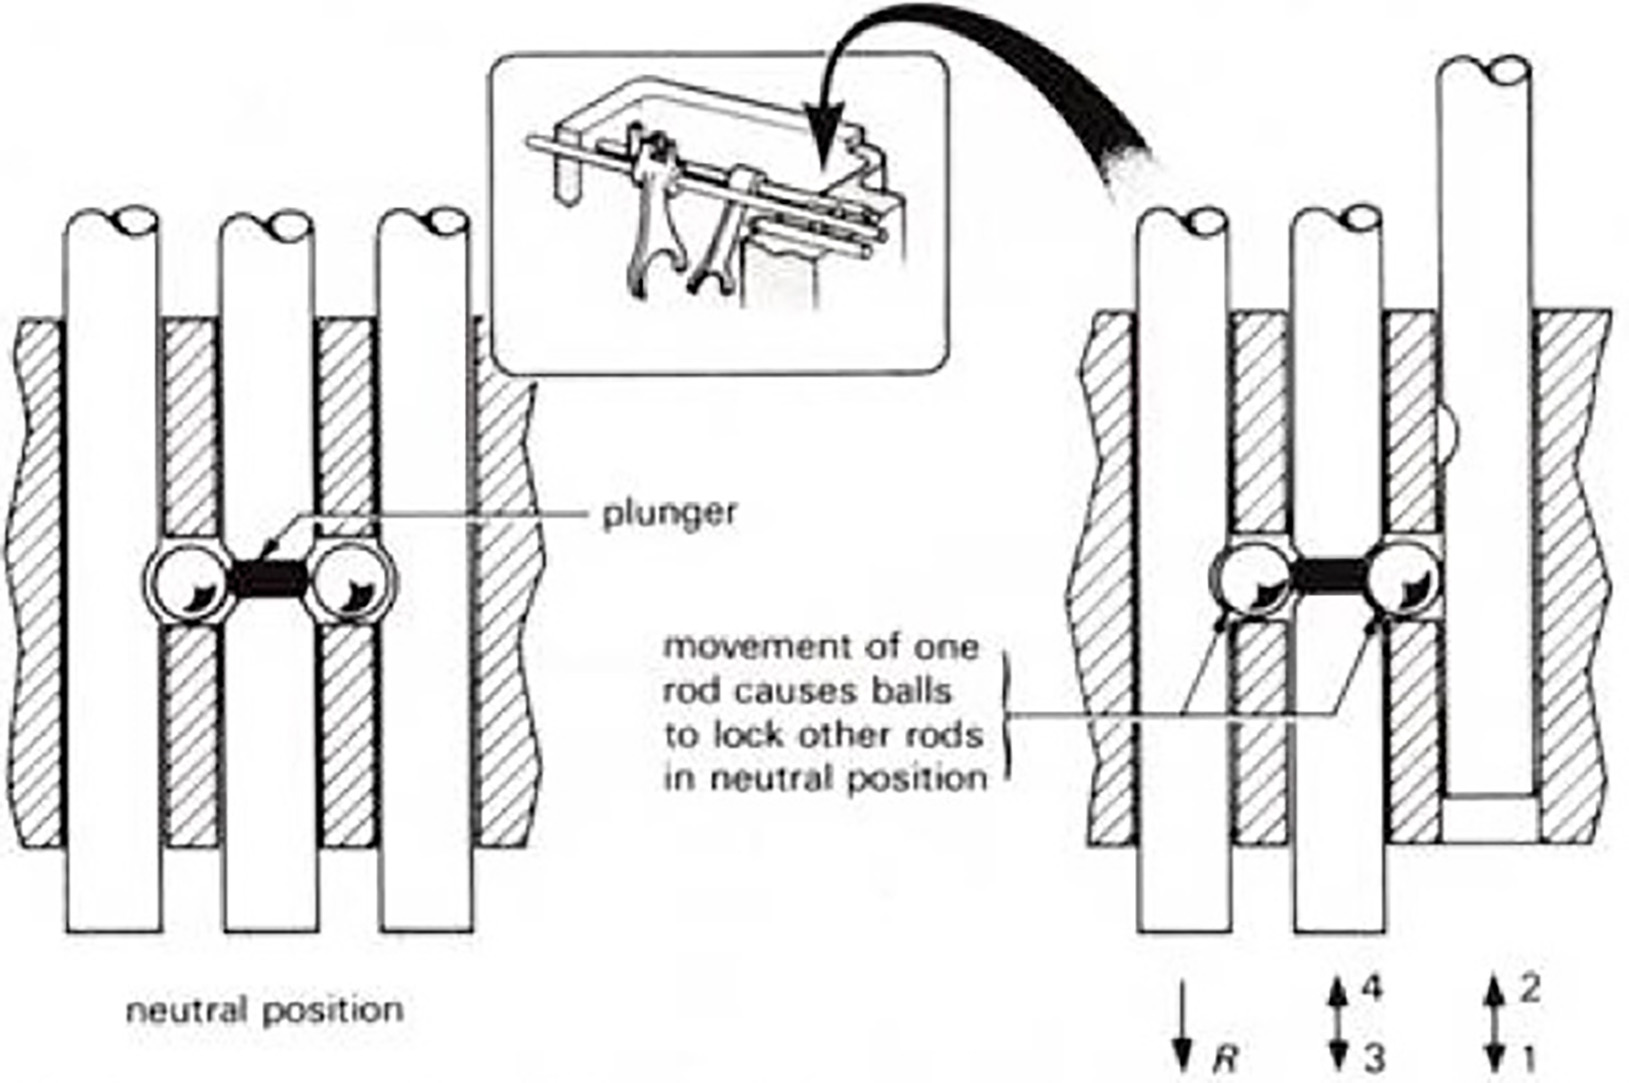
\includegraphics[width=\textwidth]{interlocking}
		\caption{互锁装置示意图}
		\label{interlocking}
	\end{minipage}
	\begin{minipage}[b]{0.3\textwidth}
		\centering
		\begin{minipage}[b]{0.8\textwidth}
			\centering
			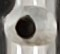
\includegraphics[width=\textwidth]{interlocking slot 34}
		\end{minipage}
		\begin{minipage}[b]{0.8\textwidth}
			\centering
			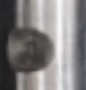
\includegraphics[width=\textwidth]{interlocking slot 5R}
		\end{minipage}
		\caption{互锁凹槽}
		\label{interlocking slots}
	\end{minipage}
\end{figure}

\subsection{试分析变速箱拆装过程的特点?}

在变速器的拆装过程中,最重要的就是记录下拆卸顺序,并在重新装配时严格按拆卸的倒序安装。

拆卸的顺序可根据各零件间相对位置关系确定。譬如说换挡轴是第一个被拆下的零件,但其上的拨杆会与5挡拨叉上的拨块干涉,需先将拨叉上的定位销取出以拆下拨叉,换挡轴在旋转一角度后便可从轴向抽出。变速器的输入轴(\cref{input shaft})和输出轴(\cref{output shaft})都是过盈装配在变速器壳体上的,拆卸时要借助压床将它们压出,压出时依次给输入、输出轴施加一小位移,并如此循环,直至两轴全被压出,注意避免让圆锥滚子轴承跳出。若一次只压一根轴,可能啮合的斜齿轮间会干涉造成齿轮损坏。输出轴被压出后,其上的1、2挡拨叉轴和拨叉才可被取下。输入轴上的3、4挡齿轮和相应的同步器由轴用挡圈轴向定位,其中固定输入轴4挡齿轮的卡簧上开有两孔,需将卡簧钳两尖头伸入孔中将卡簧撑开后提出,而固定花键毂的卡簧较厚,更好的方法是用专用的卡簧钳摩擦力较大的成平面的两侧面撑开卡簧缺口后取出。卡簧的拆装较为困难,且如果盲目撬开会造成卡簧变形,无法再装上。变速器上用到的三个定位销(\cref{location pins})为弹性圆柱销,中空且母线方向上有一贯穿的缺口。将销钉敲下时,应用磨钝尖端的螺钉抵住销钉边缘,并用锤子敲击螺钉头部。若直接让螺钉深伸入定位销中部的孔用力,可能会撑大定位销,使之难以被取出。

重新装配变速器的过程事实上较拆卸有更多需要注意的点,因为拆卸顺序错误无非是有零件无法拆下,但装配错误可能要到后面试图装其它零件时才能发现,所幸我组没有遇到此类情况。该型变速器上所用同步器的滑块靠两侧的两钢丝弹簧固定,钢丝弹簧开口的一端有一倒钩,另一端是平的。装配同步器时,先将滑块放入花键毂的凹槽中,套上接合套将滑块基本限位住后才能安装钢丝弹簧。安装钢丝弹簧时,要首先让其有钩子的一端钩住滑块背面的凹槽,然后将其余部分压入,这使得钢丝弹簧不会在同步器中周向转动,也不会从轴向脱出。注意到钢丝弹簧只有约3/4圆周长,故而在安装另一面的钢丝弹簧时注意将缺口错开,以免滑块受力不均。我们主要探究的是3、4挡同步器,这个同步器虽向两侧均能工作,分别控制3、4挡,但仔细观察会发现其花键毂的外花键是断开的,外花键两侧不等长,且花键毂的两侧毂与外花键端部的距离不等,总之花键毂并非左右对称。这种设计可能的原因是两挡受力不同,也带来了安装方向的问题。若将同步器翻转过来安装,花键毂能被装上,因为用于定位花键毂的毂翻转后长度不变,但花键毂上外花键端部的位置变了,这就会使得4挡齿轮装不上,又得把同步器整体拆下重装。所以拆卸时就应记下该同步器的方向以便后面的安装。装回输入、输出轴时,自然要和拆下时一样先把两轴摆到齿轮能啮合的位置,且输出轴要带着1、2挡拨叉轴和拨叉一道装回。然而,装回输入、输出轴时压床已不可用,因为轴伸出箱体的长度超出了压床的工作范围。我们采用的办法是将轴的一端顶在台虎钳上,另一侧用套筒顶在放入轴安装孔的轴承上,敲击套筒即可借助相对运动把输入、输出轴安装到位。倒挡轴和倒挡中间齿轮拆下时较易,仅需将倒挡轴敲出,但装入时要确定倒挡齿轮的方向,且因此时输入、输出轴已装上,倒挡齿轮放倒后才能装入,需用螺丝刀将齿轮重新挑到直立位后再装入倒挡轴。由于倒挡轴上带有定位销,装入时销钉要对准壳体上的开槽,且要从倒挡齿轮的另一侧装入,避免定位销和倒挡齿轮干涉。变速器中三个拨叉也都不是左右对称的,需按原方向安装,否则会和自锁干涉。我们的变速器中已拆掉了互锁,故两拨叉轴可同时挂入工作挡位,但为了最后变速杆安装方便和以后的拆卸,我们需将三轴均移至空挡位置。

\begin{figure}[htbp]
	\centering
	\begin{minipage}[b]{0.18\textwidth}
		\centering
		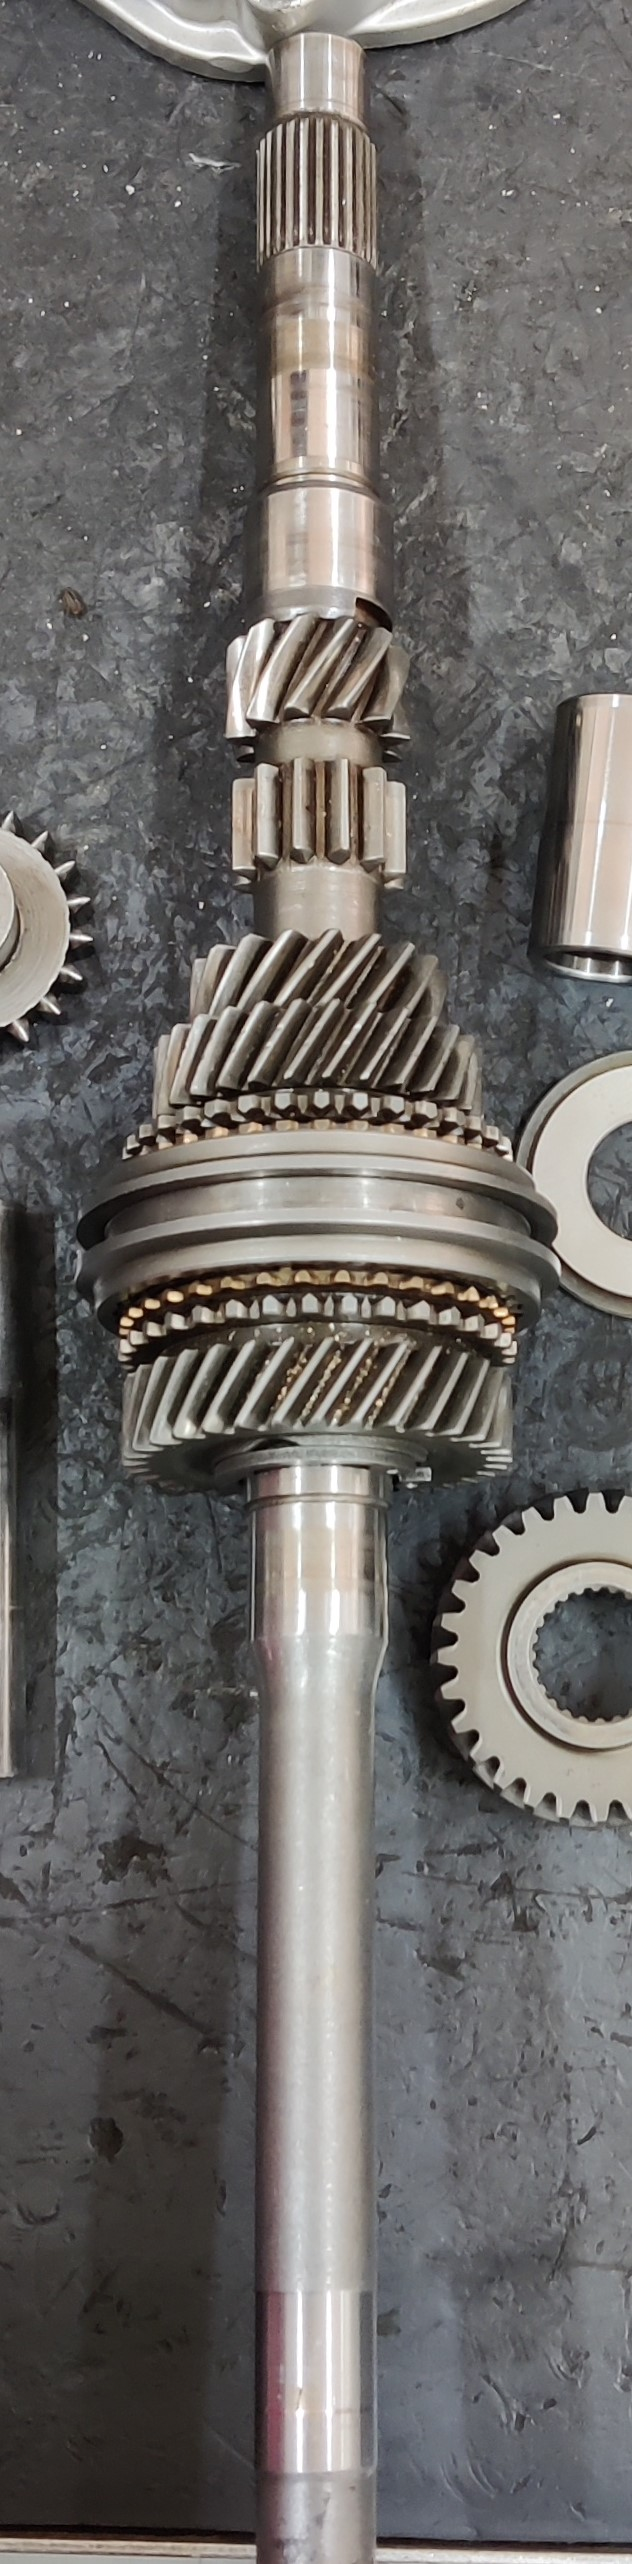
\includegraphics[width=\textwidth]{input shaft}
		\caption{输入轴}
		\label{input shaft}
	\end{minipage}
	\begin{minipage}[b]{0.31\textwidth}
		\centering
		\begin{minipage}[b]{\textwidth}
			\centering
			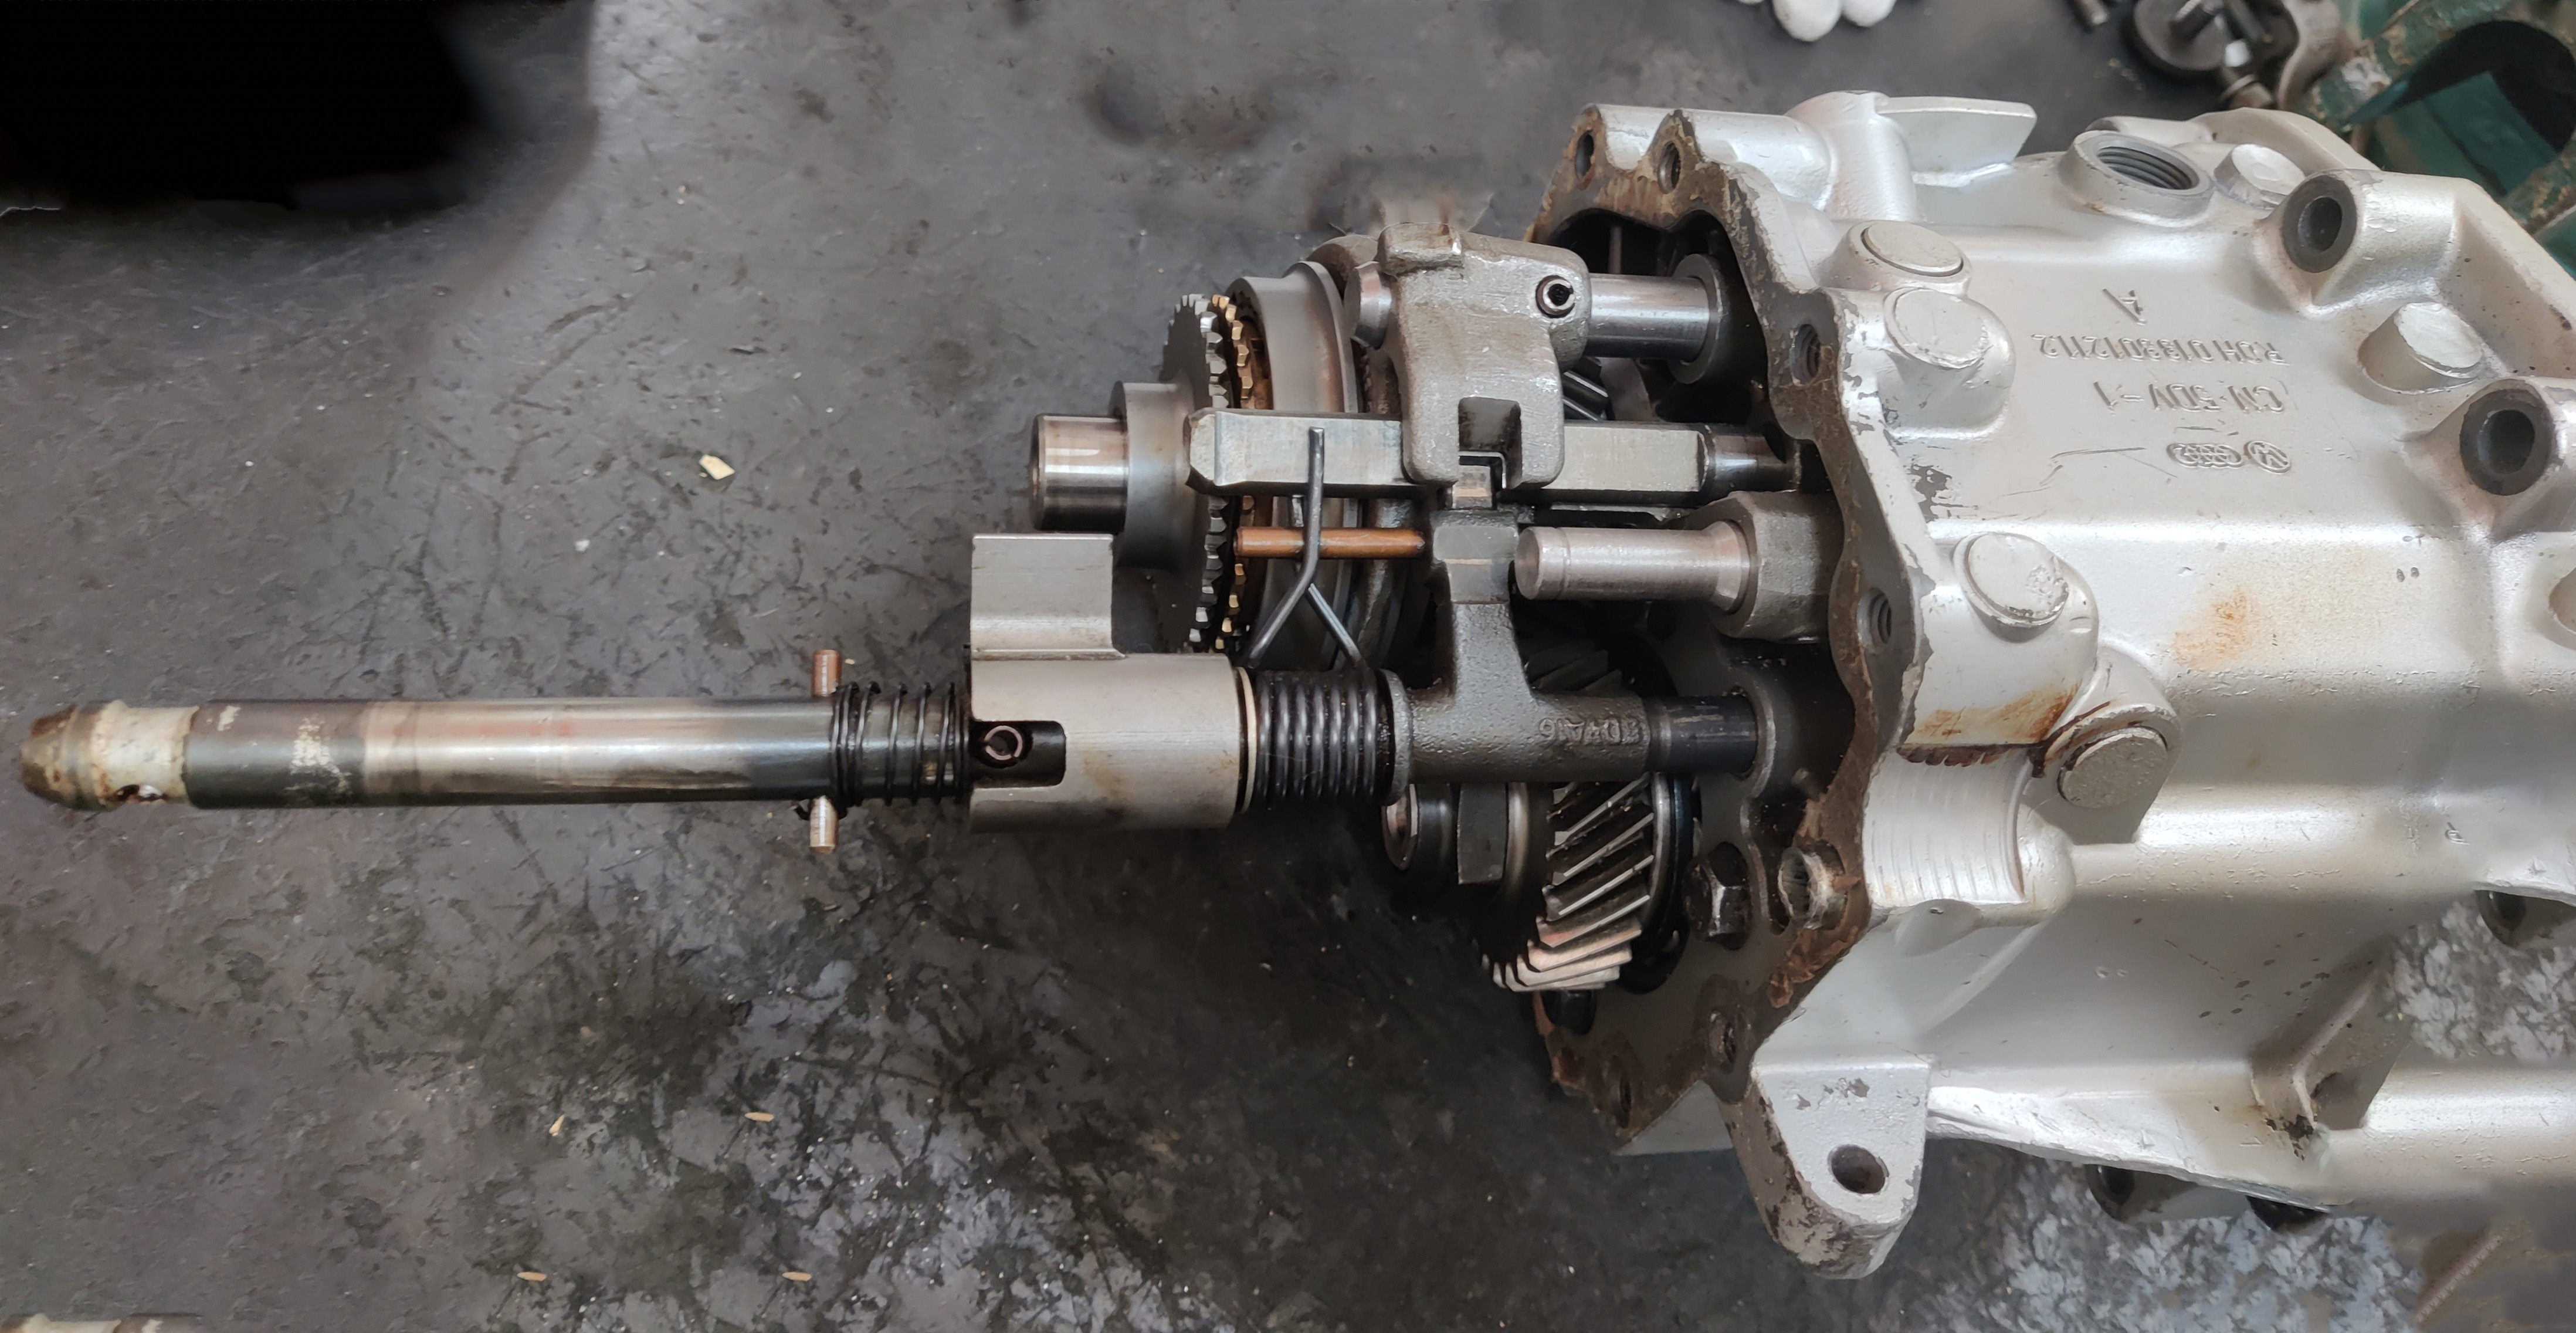
\includegraphics[width=\textwidth]{gearbox}
			\caption{变速器}
			\label{gearbox}
		\end{minipage}
		\begin{minipage}[b]{\textwidth}
			\centering
			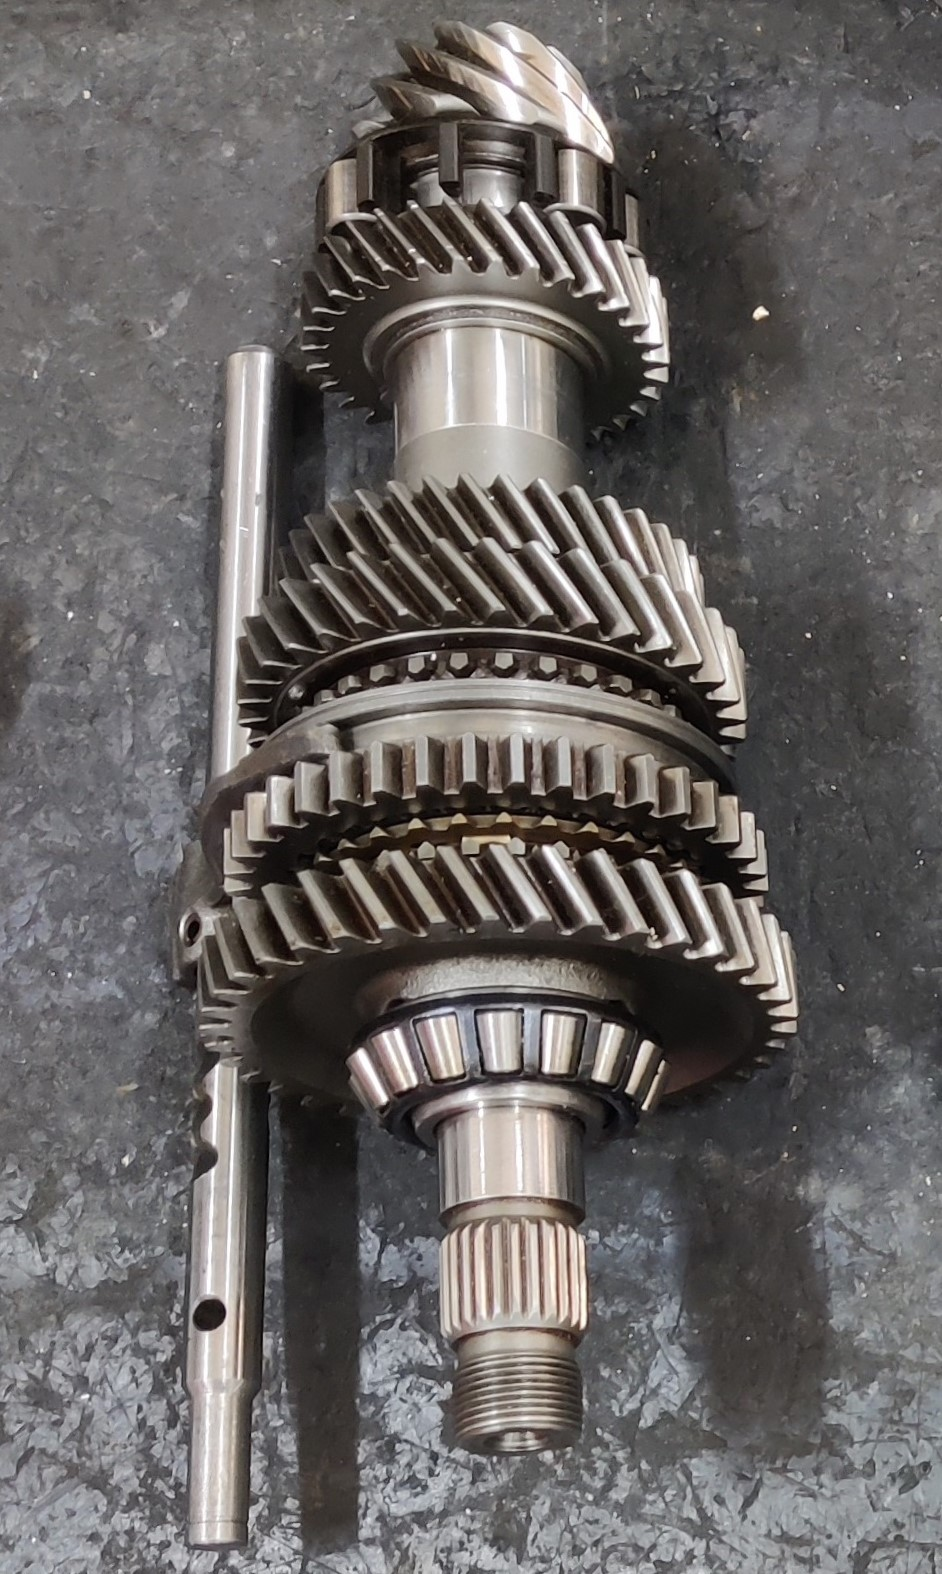
\includegraphics[width=\textwidth]{output shaft}
			\caption{输出轴}
			\label{output shaft}
		\end{minipage}
	\end{minipage}
	\begin{minipage}[b]{0.39\textwidth}
		\centering
		\begin{minipage}[b]{\textwidth}
			\centering
			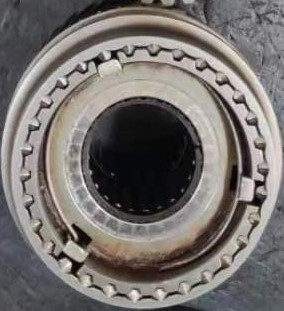
\includegraphics[width=\textwidth]{synchronous}
			\caption{同步器}
			\label{synchronous}
		\end{minipage}
		\begin{minipage}[b]{\textwidth}
			\centering
			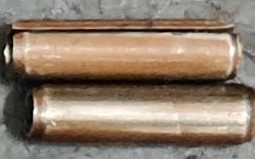
\includegraphics[width=\textwidth]{location pins}
			\caption{定位销}
			\label{location pins}
		\end{minipage}
	\end{minipage}
\end{figure}

\subsection{两轴变速器的工作原理。}

变速器的作用主要表现在三方面:第一,改变传动比,扩大驱动轮的转矩和转速的变化范围;第二,在发动机转向不变的情况下,实现汽车倒退行驶;第三,利用空挡,使得可以中断发动机动力传递,让发动机可以起动、怠速。

两轴式变速器的动力传递主要依靠两个相互平行的轴(输入轴和输出轴)完成,此外还有一根较短的倒挡轴帮助汽车实现倒退行驶。动力从第一轴输入,经一对齿轮传动后,直接由第二轴输出,故其在一般的减速挡时效率高于三轴式变速器,但无法设置高效的真正的直接挡,且输出轴转向和输入轴相反。

两轴式变速器的前进挡一般都采用常啮合斜齿轮,主动齿轮均为右旋,从动齿轮均为左旋,每对啮合斜齿轮中总有一个是空套在轴上。现在变速器的前进挡一般都采用同步器换挡,需换入某一工作挡位时拨动换挡杆,带动换挡滑块和拨叉将接合套与相应挡位空套的那个齿轮上的接合齿圈接合,使得该齿轮与输入轴或输出轴刚性连接,从而传递动力。各挡的动力传递路线已在\cref{subsection:2.1}中提到过。

为实现汽车的倒退行驶,在输入轴的一侧设置有一根较短的倒挡轴。倒挡中间齿轮空套在倒挡轴上(不用滚针轴承),可轴向滑动,空挡时与输入轴和输出轴的倒挡齿轮不在同一平面。我们在拆装实践中发现,该型变速器倒挡采用直齿滑动齿轮换挡,且输入轴倒挡齿轮、输出轴倒挡齿轮和倒挡中间齿轮在换挡时接合的那一侧都做了斜面处理,在换入倒挡时有一定的导向作用。显然换入倒挡前需先停车,故倒挡可不用接合套,拨动倒挡齿轮使其同时与输入、输出轴上两对应齿轮啮合即可。

两轴式变速器的结构简单、紧凑,容易布置,多用于前置前驱(FF)或后置后驱(RR)的普通级和中级轿车上。

\clearpage

\section{汽油机部分}
\subsection{一般的配气机构、进气门间隙和排气门间隙哪个气门间隙更大一些? 为什么?}

为给气门等部件在发动机工作时受热伸长留出空间,防止引起气门关闭不严造成汽缸漏气、功率下降,在发动机冷态装配时须在气门及其传动件之间留有适当间隙,这个间隙就是气门间隙(\cref{valve clearance}),即气门完全关闭时气门杆尾端与摇臂或挺柱之间的间隙。气门间隙可通过气门间隙调整螺钉调节,并用塞尺测量间隙是否合适。

气门间隙是因气门等受热后会膨胀而被需要的。我们拆的汽油机中采用液力挺柱(\cref{valve clearance}),因其可自动补偿间隙而毋须预留气门间隙。但采用一般的机械挺柱时材料均会受热碰撞,故均需气门间隙。由于进气门中流过的是油气混合气或新鲜空气,而排气门中流过的是燃烧后的高温废气,排气门工作温度比进气门高得多,而二者材料的热膨胀系数差别不大,故排气门部件工作时伸长量更大,需要的气门间隙也就更大。

\begin{figure}[htbp]
	\centering
	\begin{minipage}[b]{0.5\textwidth}
		\centering
		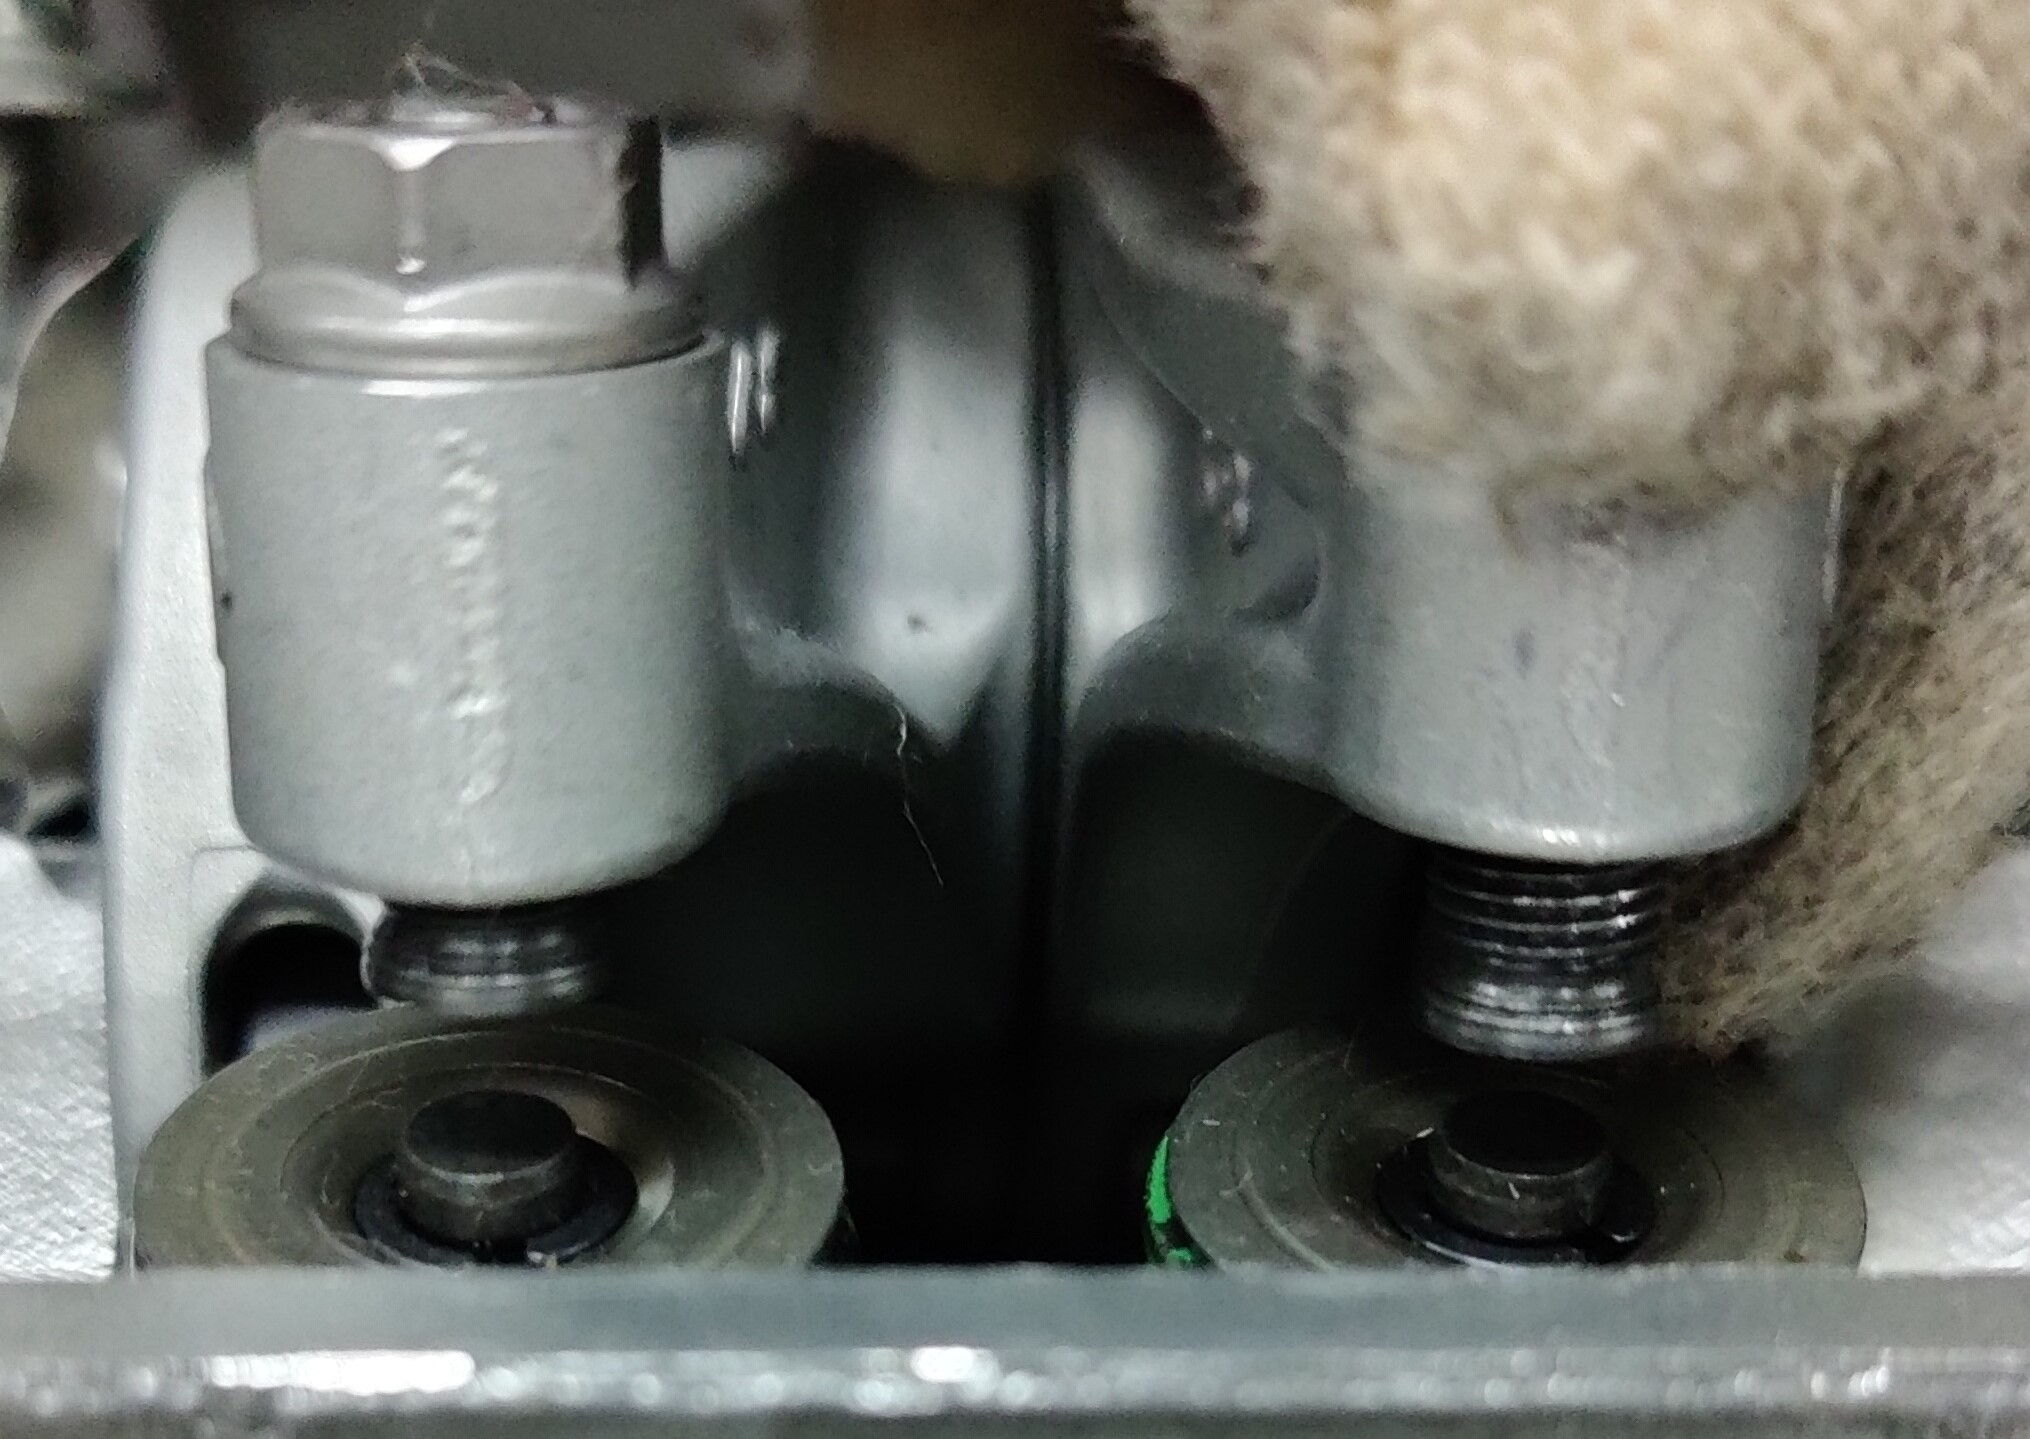
\includegraphics[width=\textwidth]{valve clearance}
		\caption{气门间隙}
		\label{valve clearance}
	\end{minipage}
	\begin{minipage}[b]{0.4\textwidth}
		\centering
		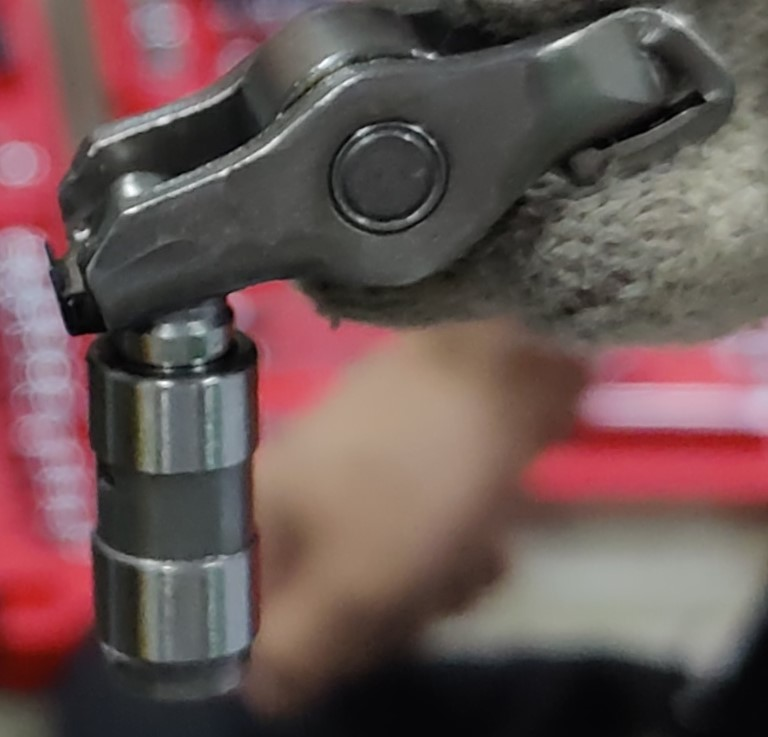
\includegraphics[width=\textwidth]{hydraulic tappet}
		\caption{液力挺柱}
		\label{hydraulic tappet}
	\end{minipage}
\end{figure}

\subsection{曲柄连杆机构由哪些零件组成?}

曲柄连杆机构由活塞连杆组和曲轴飞轮组组成。

活塞连杆组包括的零件有:活塞、活塞环(包括气环和油环)、活塞销、连杆、连杆小头衬套(采用全浮式活塞销时)、金属卡环(采用全浮式活塞销时)、连杆轴瓦、定位凸键、连杆盖、连杆螺栓等(\cref{piston and connecting rod})。

曲轴飞轮组包括:曲轴、飞轮、转速传感器脉冲轮、曲轴正时齿轮(或正时带轮、正时链轮)、曲轴带轮、扭转减振器、主轴承(包括滑动轴承和一个滑动推力轴承)、主轴承盖等(\cref{crankshaft-flywheel})。

\begin{figure}[htbp]
	\centering
	\begin{minipage}[b]{0.2\textwidth}
		\centering
		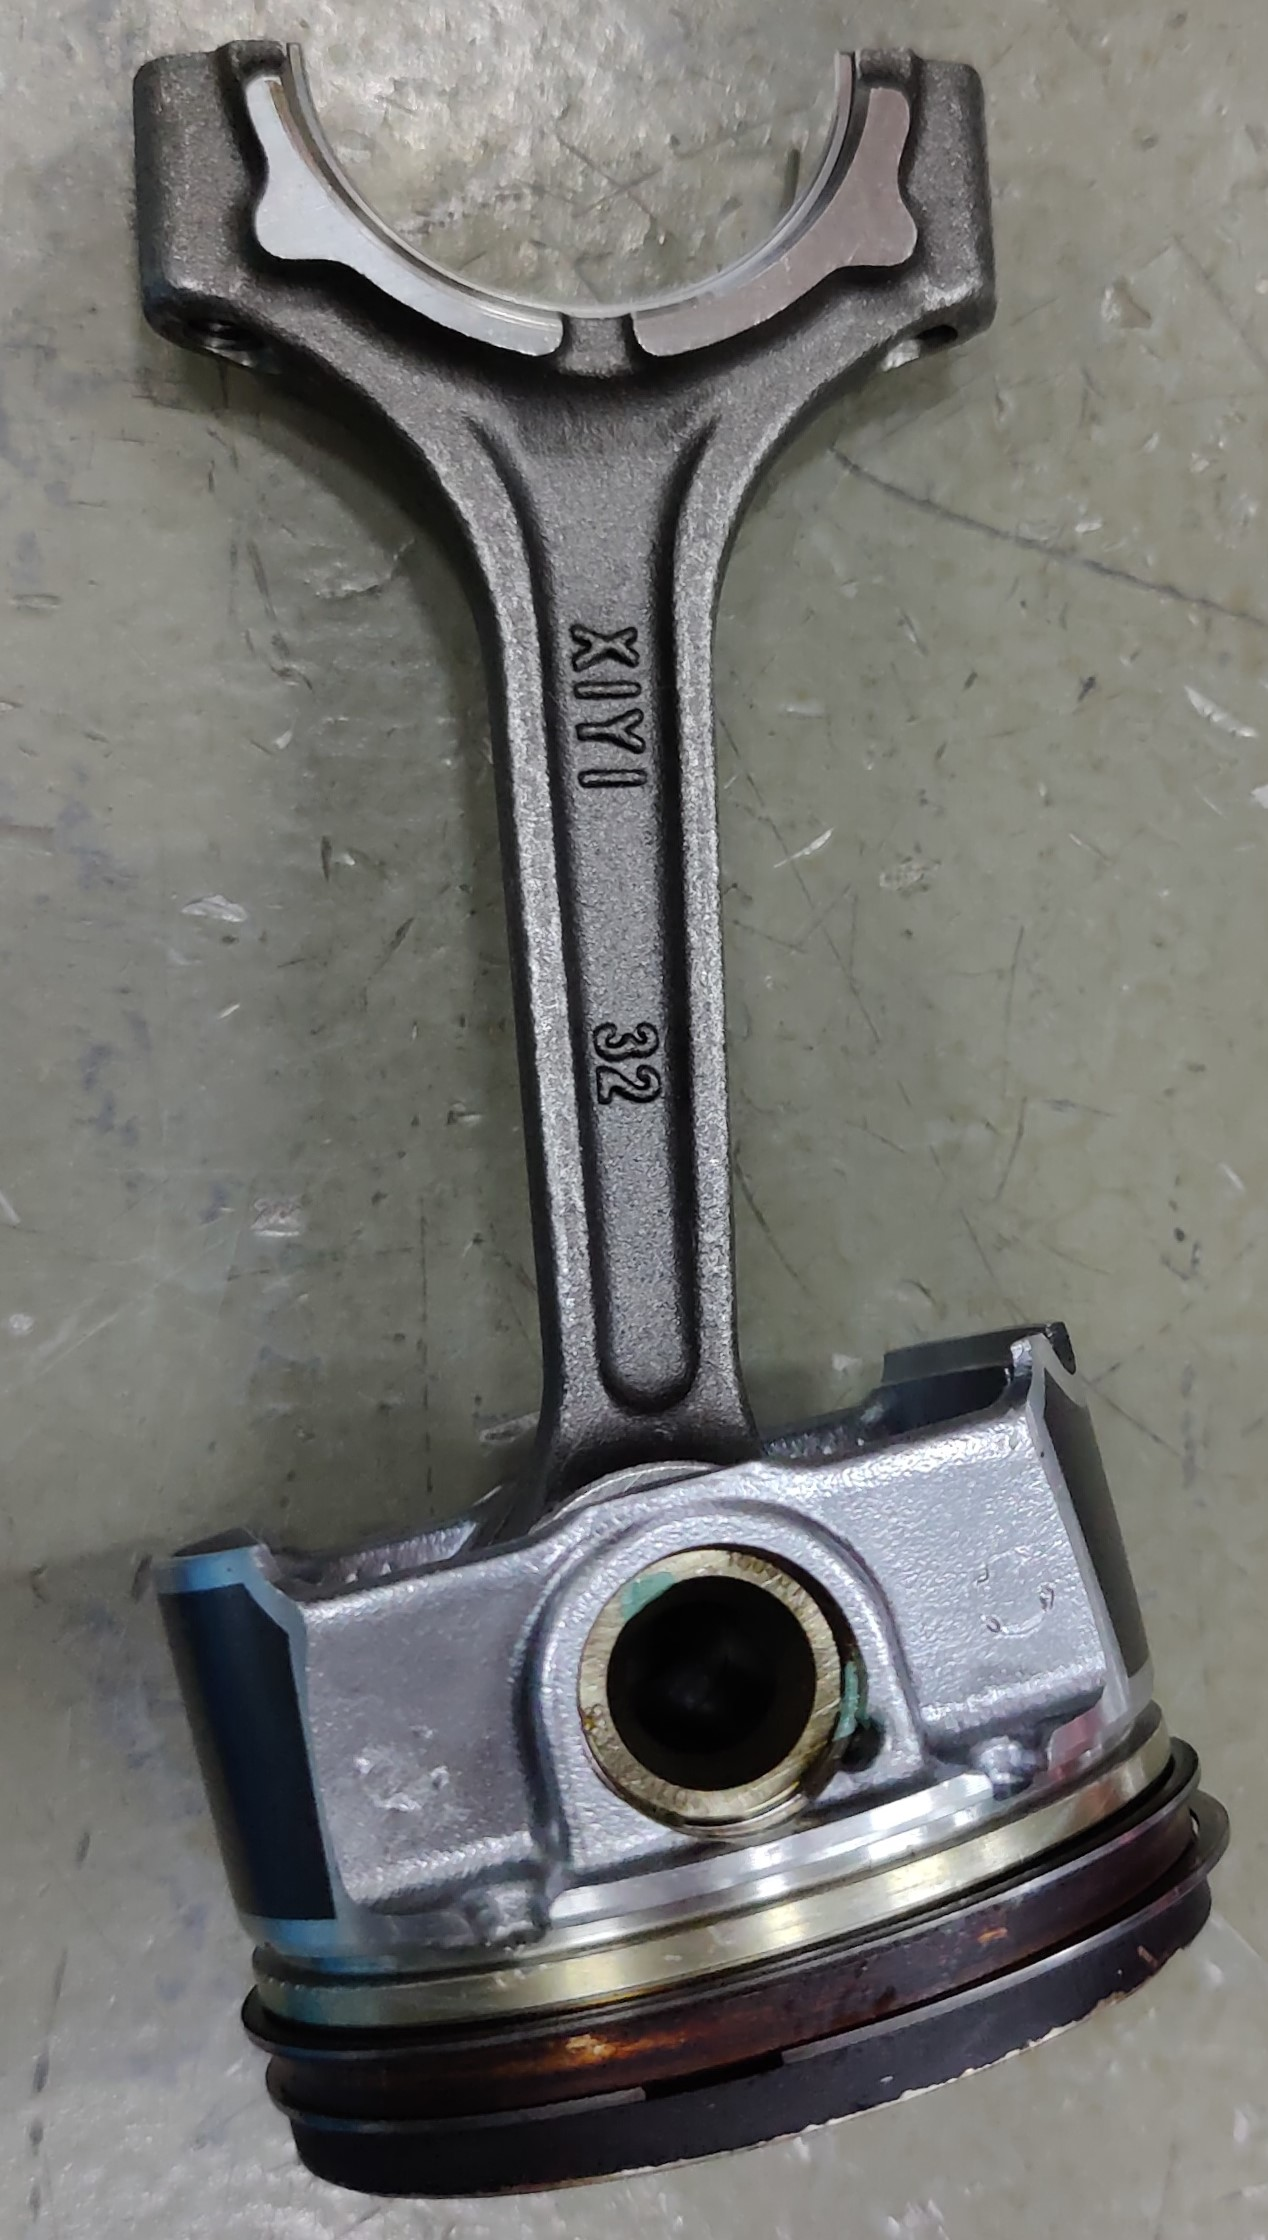
\includegraphics[width=\textwidth]{piston and connecting rod}
		\caption{活塞连杆组部分零件}
		\label{piston and connecting rod}
	\end{minipage}
	\begin{minipage}[b]{0.7\textwidth}
		\centering
		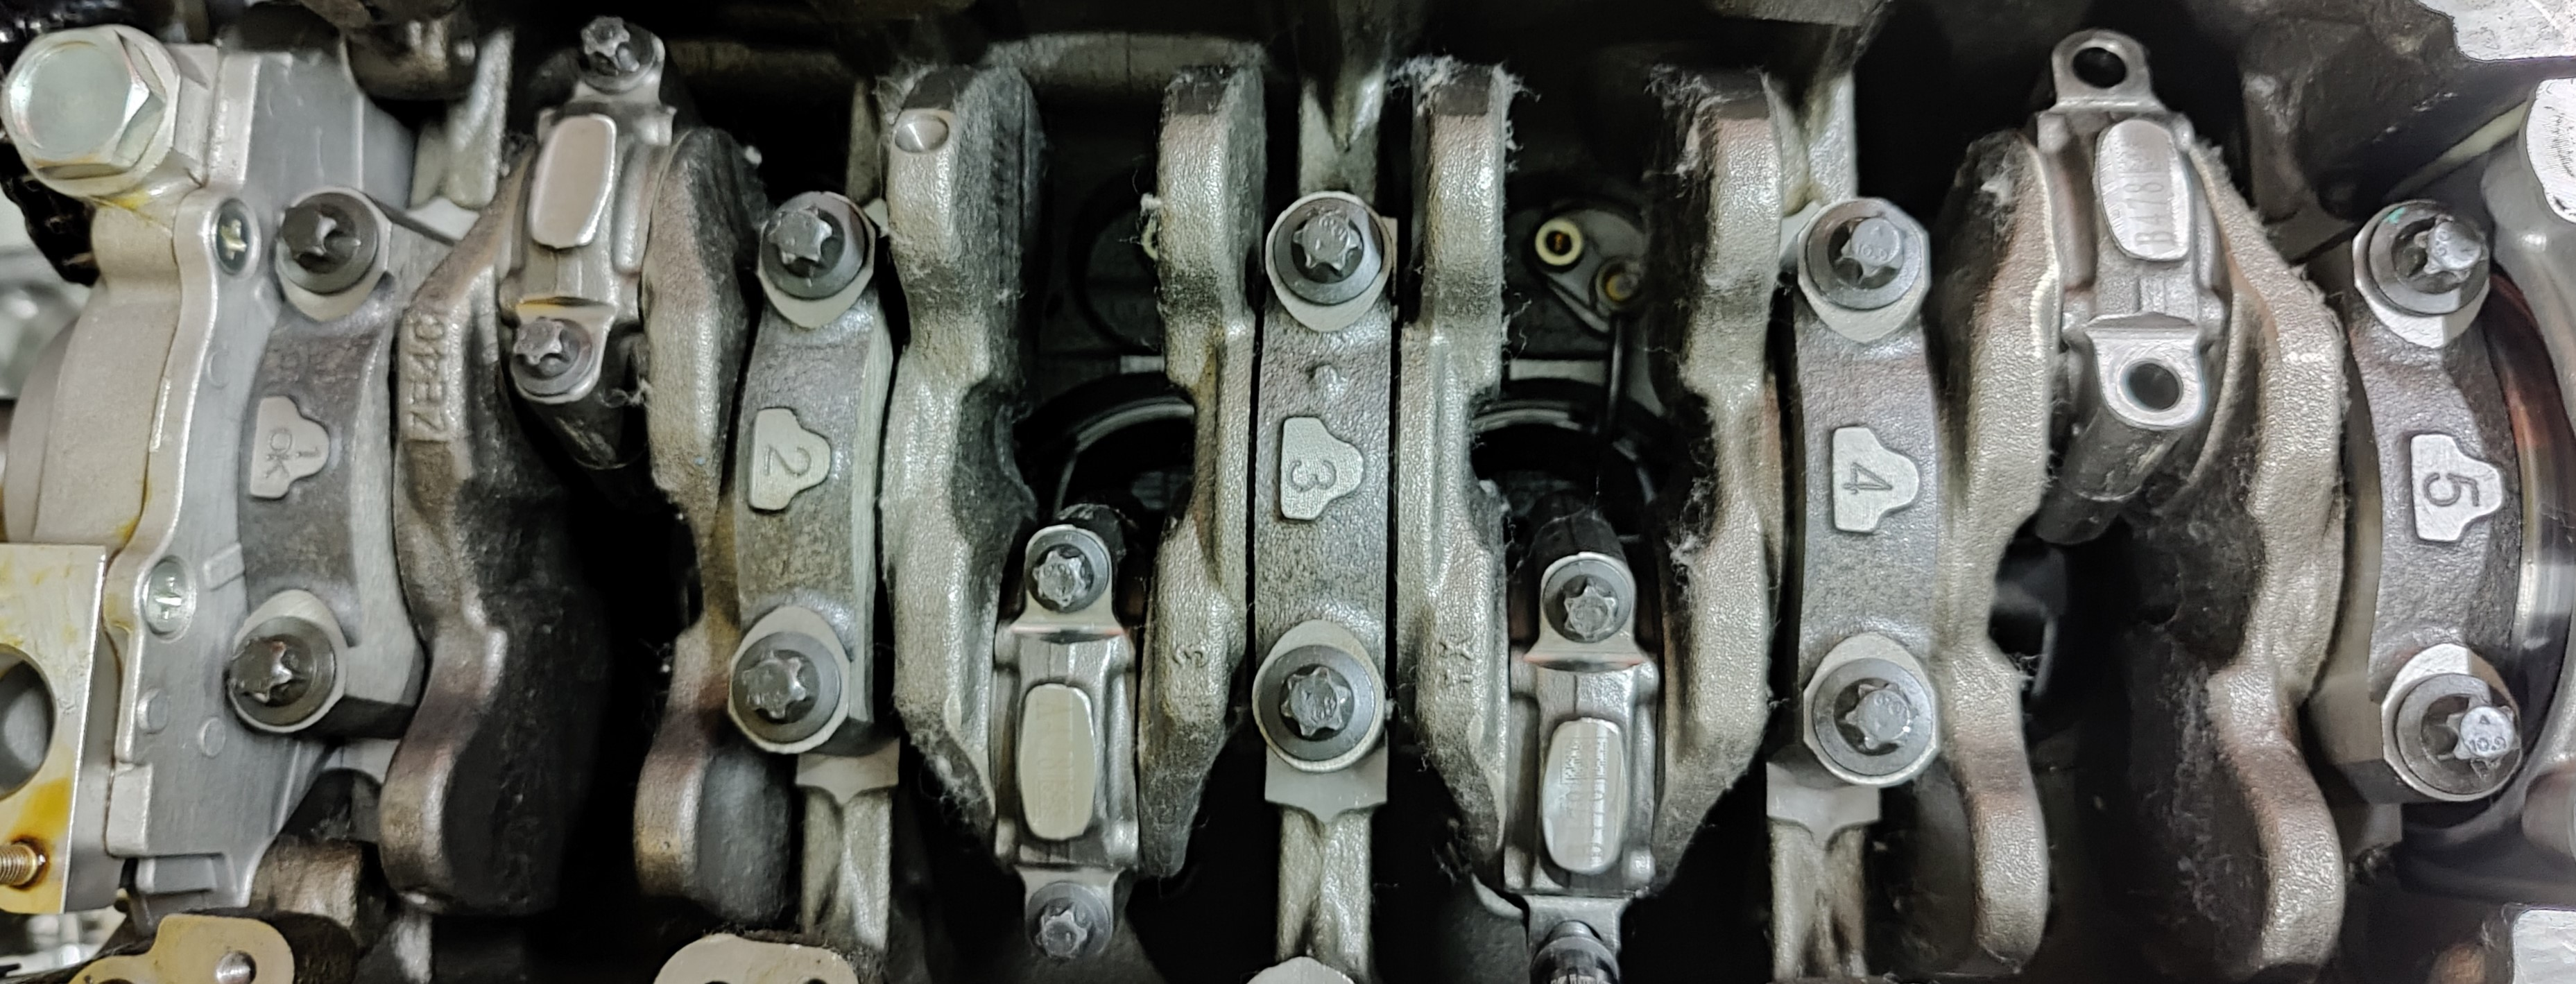
\includegraphics[width=\textwidth]{crankshaft-flywheel}
		\caption{曲轴飞轮组部分零件}
		\label{crankshaft-flywheel}
	\end{minipage}
\end{figure}

\subsection{试述活塞环的分类与作用。}

活塞环是具有弹性的开口环,分为气环和油环。

气环密封汽缸壁与活塞,防止燃烧室中高温燃气漏入曲轴箱;并将活塞从其顶部吸收的热量传给汽缸壁,防止活塞过热。

油环在上行时可帮助在汽缸壁上涂布一层均匀的润滑油;并在下行时把飞溅到汽缸壁上的多余润滑油刮除掉,既可防止机油窜入燃烧室,同时使汽缸壁上润滑油膜均匀分布,改善活塞组的润滑条件。当然,油环对封气也起到辅助作用。

气环的开口形状会直接影响漏气量,开口形状有直开口、梯形开口、斜切口等。气环按断面形状可分为矩形环、扭曲环、锥面环、梯形环和桶面环等。

油环分为普通油环和组合油环。

\subsection{安装活塞环时应注意什么?}

\begin{itemize}
	\item 安装活塞环前应充分清除积碳,防止活塞环安装后卡死在汽缸中。

	\item 安装时注意活塞环的正反。譬如扭曲环、锥面环在装反时反而会向上刮油,造成机油上窜。

	\item 先装油环。对于组合式油环,先装衬环,再装刮片。

	\item 安装气环时要用专用活塞环扩张钳将气环按环的说明书上的安装要求和方向装入环槽,先装黑色的第二道气环再装镀铬的第一道气环,如\cref{piston head}。

	\item 若采用三道活塞环,它们的开口应相互错开\SI{120}{\degree},四道活塞环时开口则应相互错开\SI{90}{\degree}。组合油环的上、下刮片开口应错开\SI{180}{\degree},且与衬环的开口应相互错开\qtyrange[range-phrase = $\,\sim\,$, range-units = single]{45}{90}{\degree}。安装时,所有的环开口还要错开活塞销孔及活塞最大侧压力的方向。如不错开,可能造成漏气、漏油量的增大。

	\item 使用活塞环扩张钳时注意用力应适当,若扩张力太大可能造成活塞环塑性变形,撑坏活塞环。

	\item 气环上缺口大小应适当,可将环试装入进汽缸体后观察测量,若不合适需进一步加工调整。

	\item 将安装好活塞环的活塞连杆组装配进汽缸之前,要用活塞环压缩器(\cref{piston ring compressor})压紧活塞环,锁紧位置约在活塞二分之一位置处。将活塞连杆组放入汽缸后继续用专用扳手锁紧少许,防止环凸出。用扳手压平活塞夹顶端平面,再将活塞从活塞环压缩器中用锤柄推入汽缸。
\end{itemize}

\begin{figure}[htbp]
	\centering
	\begin{minipage}[b]{0.6\textwidth}
		\centering
		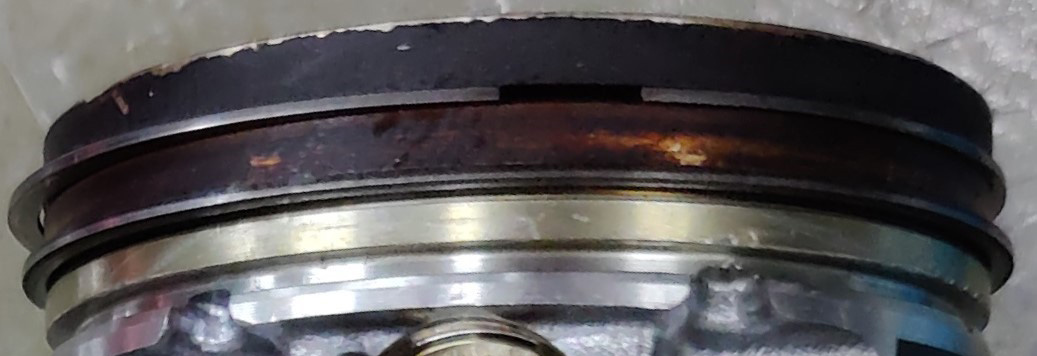
\includegraphics[width=\textwidth]{piston head}
		\caption{活塞头部}
		\label{piston head}
	\end{minipage}
	\begin{minipage}[b]{0.3\textwidth}
		\centering
		\includegraphics[width=\textwidth]{piston ring compressor}
		\caption{活塞环压缩器}
		\label{piston ring compressor}
	\end{minipage}
\end{figure}

\subsection{活塞、连杆、连杆盖组合装配时, 应注意什么?}

\begin{itemize}
	\item 装配前应选配活塞、活塞销与连杆衬套,并清洁。

	\item 清洗后的活塞连杆在装成组合件前应进行检验,包括活塞的磨损检验,活塞环的检验、选配,连杆衬套与销的检查,连杆及连杆轴瓦的检验等。

	\item 安装全浮式活塞销前,应将活塞在容器中加热。由于活塞是铝活塞,而活塞销采用钢材料,铝的热膨胀系数高于钢,为了保证高温工作时活塞销与活塞销座孔为过渡配合,常温时二者间为过盈配合,不便安装,加热活塞能使活塞销座孔变大,方便安装。当然,为活塞销降温也是可行的。半浮式活塞销和连杆小头过盈配合,安装半浮式活塞销时,应将连杆小头加热一定温度,再用专用工具把活塞销压入。若直接在常温下用锤子敲入,可能造成活塞销、活塞或连杆的变形,加剧工作时磨损。

	\item 注意要先将连杆小头放入活塞两销孔之间并对准连杆小头孔与销孔,再推动活塞销先后穿过活塞一端的销孔、连杆小头孔和活塞的另一端销孔。连杆小头孔中装配前要涂上干净的润滑脂。

	\item 全浮式活塞销在压入销孔后不要忘记按装卡环限制其轴向移动,否则工作时可能轴向窜动刮伤汽缸壁。

	\item 当不换新件时,连杆大头与连杆盖必须配对安装,不可互换,加工时二者的同一侧间已被打上配对标记。当连杆盖和连杆大头采用现在常用的胀断法加工并通过自然断裂面定位时,由于每对自然断裂面形状都不同,在定位的同时也能起到防止错装的效果。

	\item 活塞连杆体与曲轴的相对位置也不能前后装反,当活塞顶部有活塞气门干涉凹坑(\cref{piston valve interference pits})时,可根据它的方向判断,以保证活塞顶部不会和气门干涉。即使没有干涉凹坑或凹坑对称,也须按原方向安装,使得连杆大头与曲柄销之间配合良好。

	\item 连杆轴瓦上开有油孔时,应与连杆大头上相应的油孔对齐。

	\item 拧紧连杆螺栓时应交替拧紧,最好用校准过的力矩扳手控制拧紧力矩。连杆螺栓应采取适当的防松措施,譬如螺纹防松胶、防松螺母等。防松胶必须选用耐高温的牌号,防松螺母不应用不耐高温的尼龙防松螺母。

	\item 活塞与对应的汽缸间采用选配方式。装配前可测量各活塞和汽缸壁的直径,挑选出合适的配对关系。

	\item 每装好一个活塞后要转动曲轴一周,观察连杆轴瓦与曲柄销配合间隙的松紧,以及活塞在汽缸中是否偏缸。
\end{itemize}

\begin{figure}[htbp]
	\centering
	\begin{minipage}[b]{0.4\textwidth}
		\centering
		\includegraphics[width=\textwidth]{piston valve interference pits}
		\caption{活塞气门干涉凹坑}
		\label{piston valve interference pits}
	\end{minipage}
\end{figure}

\subsection{绘制润滑系统或冷却系统原理示意图(二选一) ?}

润滑系统原理示意图如\cref{lubricating system}所示。

\begin{figure}[htbp]
	\centering
	\begin{minipage}[b]{\textwidth}
		\centering
		\includegraphics[width=\textwidth]{lubricating system}
		\caption{润滑系统原理示意图}
		\label{lubricating system}
	\end{minipage}
\end{figure}

\clearpage

\section{柴油机部分}
\subsection{请简述柴油机工作原理}

1897年,Rudolf Diesel制造出他的第一台著名的高压缩发动机原型。在柴油机中,燃料燃烧产生的高温使高压气体膨胀,进而推动活塞,将化学能转化为机械能。

汽缸中每一次将热能转变为机械功的一系列连续过程为一个工作循环。柴油机一般为四冲程。四冲程柴油机的一个工作循环中,包括进气、压缩、做功(燃烧——膨胀)、排气四个行程。其中,只有做功行程中发动机对外做功,并在其它三个行程借助惯性或同一发动机中其它缸做功产生的动力克服压缩阻力和摩擦阻力,连续运转。

发动机有一最低稳定转速,称为怠速。怠速运转时,喷油量较小,柴油燃烧产生的热量恰可克服发动机内部的阻力,实现发动机的连续稳定运转,此时发动机不对外做功。发动机的起动需靠外部能量,现在一般采用起动电机,电机的输出连到曲轴上的飞轮,将发动机带至起动转速。一般发动机的起动转速比怠速低得多,柴油机的起动转速为\qtyrange[range-phrase = $\,\sim\,$, range-units = single]{150}{300}{\rpm},但起动时喷油量很大,发动机可以顺利起动,过渡到稳定运行状态。

柴油机的工作原理通过进气、压缩、做功和排气四个行程说明:

\begin{itemize}
	\item 进气行程:曲轴旋转,活塞从上止点向下止点运动,此时排气门关闭,进气门打开。随着活塞下移,汽缸内容积增大,这就在缸内产生真空度,将外界新鲜空气经进气系统,通过进气门吸入汽缸。当活塞运动到下止点附近,进气行程结束。

	\item 压缩行程:曲轴继续旋转,活塞由下止点向上止点运动,进、排气门都关闭,汽缸内近似为一密封环境。进气行程吸入的新鲜空气和上一工作循环中残余的部分废气被压缩,压力和温度升高。当活塞接近上止点时,喷油器开始喷油,将高压柴油以雾状喷入燃烧室,雾状柴油在燃烧室中迅速蒸发,与空气形成可燃混合气,经过短暂的备燃期之后自行发火燃烧,无需点火。柴油机的压缩比较大,可达\numrange[range-phrase = $\,\sim\,$]{16}{24},故压缩终了时气体的温度和压力也较高,温度可达\qtyrange[range-phrase = $\,\sim\,$, range-units = single]{750}{1000}{\kelvin},压力达\qtyrange[range-phrase = $\,\sim\,$, range-units = single]{3.5}{4.5}{\mega\pascal},能满足柴油被压燃的外部条件。

	\item 做功行程:做功行程包括燃烧和膨胀过程,进、排气门均关闭。混合气被压燃后迅速燃烧放出大量的热,使缸内气体温度和压力急剧升高,经速燃期后,缸内压力达到最大。高温高压气体推动活塞从上止点向下止点运动,通过连杆系将活塞的直线运动转化为曲轴的旋转。发动机通过曲轴输出动力,维持发动机本身运转,并对外做功。随着活塞向下运动,汽缸内容积增加,柴油处于缓燃期,此时压力已开始下降,但温度仍上升。缓燃期结束时温度达到最大值,而后活塞继续下行,气体压力和温度均降低。发动机排气门一般设有一早开角,在活塞运动到下止点前就将排气门打开,利用此时缸内较高的压力推动部分废气排出汽缸。活塞运动到下止点时,做功行程结束。

	\item 排气行程:由于做功行程时排气门已开启,而进气门保持关闭,活塞到达下止点后向上止点运动,燃烧后的废气在自身压力和活塞的推动下经排气门排出。活塞运动到上止点前进气门即打开,利用气门重叠效应扫出废气,同时提高充气效率。活塞越过上止点后,排气门关闭,排气行程结束。由于燃烧室容积的存在,不可能将废气全部排出汽缸。受排气阻力的影响,排气终了时,气体压力仍高于大气压力。
\end{itemize}

\subsection{请简述柴油机与汽油机之间的区别}

\begin{itemize}
	\item 可燃混合物的形成不同。

	      汽油的沸点低,易气化,很容易与空气形成均匀混合气。这就是为什么非缸内直喷汽油机在进气行程中吸入的是已预混好的可燃混合气。柴油的沸点为\qtyrange[range-phrase = $\,\sim\,$, range-units = single]{180}{360}{\celsius},不宜在缸外预混。即使加热后能在缸外气化混合,加热过程也会消耗额外的能量,且加热引起空气密度降低,会降低充气效率。因此,柴油机很早就采用了缸内直喷技术,进气行程仅吸入新鲜空气,并在压缩行程快结束时把高压燃油直接喷射到燃烧室内,与空气雾化混合形成浓度分层的混合气。

	\item 着火方式、燃烧过程不同。

	      传统汽油机在缸外形成预制的均质混合气后,空燃比一般控制在理论空燃比附近,若此时尝试将混合气压燃,混合气将同时着火,缸内压力急剧升高,类似于爆炸,可能损坏活塞、连杆等部件。因此,汽油机宜采用外源强制点火燃烧的方式,即先在火花塞附近高温点火,然后让火焰在缸内传播,直至点燃所有混合气。当然,在混合气很稀薄的情况下汽油压燃也是可行的,譬如马自达的e-SKYACTIV X发动机结合了高压缩比和超稀薄燃烧,燃烧更为均匀、充分。

	      柴油的着火温度较低,柴油机从开始喷油到喷出的柴油自燃的时间较短,同一时刻适合燃烧的混合气体量不大,初期工作粗暴的问题不明显。在初期着火燃烧后,紧接着进行边喷油、边气化、边混合的扩散燃烧,并对外做功。柴油压燃并不会产生汽油机那样工作粗暴的问题,适合采用压燃的着火方式,若用点燃则会增加控制难度,且没必要。

	\item 负荷调节方式不同。

	      汽油的均匀混合气能被点燃的过量空气系数范围约为\numrange[range-phrase = $\,\sim\,$]{0.4}{1.4},这个范围较小,一般通过改变节气门的开度,控制混合气的总量来调节负荷,这种方式称为负荷的量调节。

	      柴油机中柴油在喷出后还未混合均匀时就已被压燃,只要喷束附近的空燃比满足发火条件即可,故在喷油量较大的变化范围内,喷束内都能形成适合着火的混合气。因此,柴油机在一个很大的空燃比变化范围内都可实现压燃着火,可以通过调节一次工作循环中喷油量的多少来调节负荷。而工作循环中进气量基本保持不变,平均的过量空气系数会随负荷变化而变化。这种依靠改变喷油量,即改变平均的过量空气系数来调节负荷的方式,称为负荷的质调节。

	\item 活塞连杆组结构不同。

	      柴油机压缩比大,输出转矩高,曲轴的连杆轴颈较大,一般用斜切的连杆大头,活塞用铸铁制;汽油机转速高,但扭矩较小,多用平切的连杆大头,活塞也较多采用铝制。汽油机的燃烧室一般为统一式燃烧室,用于农用机械等的柴油机可用分隔式燃烧室,降低对喷油压力的要求以节约成本。柴油机压缩比大,燃烧室基本全在活塞顶部,一般用凹顶活塞;汽油机压缩比小,出于气流顺畅等因素考虑多用平顶活塞,但在一些气门升程大的汽油机中需在活塞顶铣出凹坑防止运动干涉。

	\item 排放污染控制系统不同。

	      柴油机中一般为富氧环境,产生的废气中虽污染物的总量较小,但\ce{NO_x}占比较大,造成废气中氧化剂过量,不能像汽油机那样利用三元催化转换器让废气中的\ce{CO}、\ce{HC}还原\ce{NO_x},需另加尿素等还原剂通过选择性催化还原(SCR)降低尾气中\ce{NO_x}含量。柴油机几乎全部采用缸内直喷技术,柴油和空气混合时间很短,难以充分混合造成部分燃料不完全燃烧产生以\ce{C}颗粒为主体的黑烟,一般需用颗粒捕集系统捕集炭粒以满足颗粒物的排放法规。汽油机的污染控制系统稍显简单,现在一般通过空燃比的闭环控制令混合气始终保持在理论空燃比附近,这样在排气管中用一个三元催化转换器便能完成对尾气中\ce{CO}、\ce{HC}和\ce{NO_x}的处理。目前越来越多的汽油机也开始采用缸内直喷,这同样会带来颗粒物排放增多的问题,随着法规中对汽油机颗粒物排放要求的落实,很多直喷汽油机也要采用颗粒捕集器。汽油的蒸发性较好,需用碳罐吸附油箱中挥发出的汽油,并通入进气管,最终在汽缸内烧掉;但柴油挥发较少,一般不需碳罐。当然,EGR等其它很多污染控制装置在汽、柴油机上都能够发挥作用。

	\item 从总体看,柴油机相较于汽油机的压缩比高,热效率高,燃油消耗率低,加之一般柴油的价格较低,因此柴油机的燃油经济性较好。现代柴油机的排气污染少,排放性能好,且克服了传统柴油机转速低、质量大、噪声大、振动大等缺点,只是先进柴油机的制造费用较高。
\end{itemize}

\subsection{请简述柴油机的构造(按照机构逐项说明)}

\begin{itemize}
	\item 机体组:汽缸盖罩、汽缸盖(\cref{valve and cylinder head})、汽缸垫、汽缸套、汽缸体、油底壳、链条导向板、放油螺钉、油封垫片等。

	      \begin{figure}[htbp]
		      \centering
		      \begin{minipage}[b]{0.4\textwidth}
			      \centering
			      \includegraphics[width=\textwidth]{valve and cylinder head}
			      \caption{气门、汽缸盖等}
			      \label{valve and cylinder head}
		      \end{minipage}
	      \end{figure}

	\item 曲柄连杆机构:活塞(\cref{piston and connecting rod diesel})、活塞环(包括气环和油环)、活塞销、连杆(\cref{piston and connecting rod diesel})、连杆小头衬套(采用全浮式活塞销时)、金属卡环(采用全浮式活塞销时)、连杆轴瓦、定位凸键、连杆盖(\cref{piston and connecting rod diesel})、连杆螺栓、曲轴(\cref{crankshaft})、飞轮(\cref{flywheel})、转速传感器脉冲轮、曲轴正时齿轮(或正时带轮、正时链轮)、曲轴带轮、扭转减振器、主轴承(包括滑动轴承和一个滑动推力轴承)、主轴承盖等。

	      \begin{figure}[htbp]
		      \centering
		      \begin{minipage}[b]{0.25\textwidth}
			      \centering
			      \includegraphics[width=\textwidth]{piston and connecting rod diesel}
			      \caption{活塞、连杆等}
			      \label{piston and connecting rod diesel}
		      \end{minipage}
		      \begin{minipage}[b]{0.45\textwidth}
			      \centering
			      \includegraphics[width=\textwidth]{crankshaft}
			      \caption{曲轴}
			      \label{crankshaft}
		      \end{minipage}
		      \begin{minipage}[b]{0.25\textwidth}
			      \centering
			      \includegraphics[width=\textwidth]{flywheel}
			      \caption{飞轮}
			      \label{flywheel}
		      \end{minipage}
	      \end{figure}

	\item 配气机构:正时齿形带(或正时链)、凸轮轴正时齿型带轮(或正时链轮、正时齿轮)、凸轮轴、凸轮、挺柱、推杆(\cref{pushrod})、摇臂(\cref{rocker arm})、摇臂轴、气门间隙调整螺钉、气门座圈、气门(\cref{valve and cylinder head})、气门导管、气门弹簧、气门弹簧座、锁夹等。

	      \begin{figure}[htbp]
		      \centering
		      \begin{minipage}[b]{0.7\textwidth}
			      \centering
			      \includegraphics[width=\textwidth]{pushrod}
			      \caption{推杆}
			      \label{pushrod}
		      \end{minipage}
		      \begin{minipage}[b]{0.2\textwidth}
			      \centering
			      \includegraphics[width=\textwidth]{rocker arm}
			      \caption{摇臂}
			      \label{rocker arm}
		      \end{minipage}
	      \end{figure}

	\item 进气系统:空气滤清器(\cref{air filter})、进气管、废气涡轮增压器(或机械增压器)、中冷器、空气流量计、进气温度传感器、进气歧管等。

	      \begin{figure}[htbp]
		      \centering
		      \begin{minipage}[b]{0.4\textwidth}
			      \centering
			      \includegraphics[width=\textwidth]{air filter}
			      \caption{空气滤清器}
			      \label{air filter}
		      \end{minipage}
	      \end{figure}

	\item 燃油供给系统:柴油箱(\cref{fuel tank})、输油管(\cref{diesel pipe})、油水分离器、一级输油泵、柴油滤清器(\cref{diesel filter})、二级输油泵、调速器(包括飞锤(\cref{flyweight})、调速杠杆(\cref{governor})、调速器传动齿轮、调速手柄、调速弹簧等)、分配式喷油泵、喷油提前器、喷油器、喷油泵(\cref{piston pump})、回油管(\cref{diesel pipe})等。现在多用的燃油共轨系统,包括ECU、曲轴转速传感器、凸轮轴转速传感器、加速踏板位置传感器、增压传感器、共轨压力传感器、冷却液温度传感器、低压油泵、低压油管、高压油泵、油轨、高压油管、限压阀、喷油器、回油管等。

	      \begin{figure}[htbp]
		      \centering
		      \begin{minipage}[b]{0.34\textwidth}
			      \centering
			      \includegraphics[width=\textwidth]{fuel tank}
			      \caption{油箱}
			      \label{fuel tank}
		      \end{minipage}
		      \begin{minipage}[b]{0.35\textwidth}
			      \centering
			      \includegraphics[width=\textwidth]{diesel pipe}
			      \caption{柴油油管}
			      \label{diesel pipe}
		      \end{minipage}
		      \begin{minipage}[b]{0.25\textwidth}
			      \centering
			      \includegraphics[width=\textwidth]{diesel filter}
			      \caption{柴油滤清器}
			      \label{diesel filter}
		      \end{minipage}
		      \begin{minipage}[b]{0.35\textwidth}
			      \centering
			      \includegraphics[width=\textwidth]{flyweight}
			      \caption{飞锤}
			      \label{flyweight}
		      \end{minipage}
		      \begin{minipage}[b]{0.24\textwidth}
			      \centering
			      \includegraphics[width=\textwidth]{governor}
			      \caption{调速杠杆等}
			      \label{governor}
		      \end{minipage}
		      \begin{minipage}[b]{0.35\textwidth}
			      \centering
			      \includegraphics[width=\textwidth]{piston pump}
			      \caption{柱塞泵}
			      \label{piston pump}
		      \end{minipage}
	      \end{figure}

	\item 排气及排放污染控制系统:排气歧管、排气管、前氧传感器、氧化催化剂、连续再生捕集器、选择性催化还原转化器、EGR阀、废气再循环控制阀、二级氧化催化剂、排气消声器(\cref{exhaust silencer})、排气尾管、强制曲轴箱通风、油气分离器(\cref{air oil separator})等。

	      \begin{figure}[htbp]
		      \centering
		      \begin{minipage}[b]{0.3\textwidth}
			      \centering
			      \includegraphics[width=\textwidth]{exhaust silencer}
			      \caption{排气消声器}
			      \label{exhaust silencer}
		      \end{minipage}
		      \begin{minipage}[b]{0.5\textwidth}
			      \centering
			      \includegraphics[width=\textwidth]{air oil separator}
			      \caption{油气分离器}
			      \label{air oil separator}
		      \end{minipage}
	      \end{figure}

	\item 冷却系统:水泵、冷却水管、散热器、冷却风扇、节温器、水箱(\cref{water tank})、发动机机体和缸盖上的水套、空调暖风热交换器、冷却水位传感器、冷却液温度传感等。

	      \begin{figure}[htbp]
		      \centering
		      \begin{minipage}[b]{0.5\textwidth}
			      \centering
			      \includegraphics[width=\textwidth]{water tank}
			      \caption{水箱}
			      \label{water tank}
		      \end{minipage}
	      \end{figure}

	\item 润滑系统:集滤器、机油油管(\cref{lubricating oil pipe})、机油泵、溢流阀、机油滤清器、旁通阀、机油冷却器、机油压力调节阀、主油道、曲轴油道、汽缸盖油道、机油加注口、机油尺、机油温度传感器等。

	      \begin{figure}[htbp]
		      \centering
		      \begin{minipage}[b]{0.7\textwidth}
			      \centering
			      \includegraphics[width=\textwidth]{lubricating oil pipe}
			      \caption{机油油管}
			      \label{lubricating oil pipe}
		      \end{minipage}
	      \end{figure}

	\item 起动系统:蓄电池、起动电机、起动开关、继电器、起动机电磁开关、起动机的传动机构、单向离合器、电热塞,减压装置、进气道预热装置等。

	\item 其它附件:发电机、继电器、空调压缩机、吊环螺钉(\cref{eye bolt})、铭牌、发动机悬置等。

	      \begin{figure}[htbp]
		      \centering
		      \begin{minipage}[b]{0.5\textwidth}
			      \centering
			      \includegraphics[width=\textwidth]{eye bolt}
			      \caption{吊环螺钉}
			      \label{eye bolt}
		      \end{minipage}
	      \end{figure}
\end{itemize}

\clearpage

\section{汽车电子部分}
\subsection{简述 ABS 系统组成及工作原理。}

制动防抱死系统(ABS)主要由轮速传感器、制动压力调节器和电子控制器(ECU)三大部分组成,如\cref{ABS components}所示。

汽车制动时,首先由轮速传感器测出制动车轮轮速,并将信号送入ECU。ECU中的运算单元计算出车轮速度、滑动率及车轮的加速度,然后由ECU中的控制单元对这些信号加以分析比较,向压力调节器发出制动压力控制指令。压力调节器中的电磁阀直接或间接地控制制动压力的增减,以调节制动器的制动力矩,使之与地面附着状况相适应,防止制动轮抱死。上述过程如\cref{ABS control process}。

ECU中还有故障诊断单元,其作用为对ABS各部件功能进行监测,当有部件工作异常时,通过指示灯或蜂鸣器向驾驶员发出警告,同时令整个ABS系统停止工作,恢复常规制动方式以保证基本的制动功能。

按ABS系统中可以独立进行制动压力调节的管路(通道)数可将ABS分为四通道ABS、三通道ABS、二通道ABS和单通道ABS等。通道数多的对制动压力调节更精细,制动效能更高。

\begin{figure}[htbp]
	\centering
	\begin{minipage}[b]{0.8\textwidth}
		\centering
		\includegraphics[width=\textwidth]{ABS components}
		\caption{ABS系统的组成}
		\label{ABS components}
	\end{minipage}
	\begin{minipage}[b]{0.8\textwidth}
		\centering
		\includegraphics[width=\textwidth]{ABS control process}
		\caption{ABS系统的控制过程}
		\label{ABS control process}
	\end{minipage}
\end{figure}

ABS系统的执行器——液压制动压力调节器(HCU)根据工作原理的不同可分为流通调压式和变容调压式,目前多用流通调压式HCU,它由电磁阀、液压泵和电动机等组成,直接安装在汽车原有的制动管路中,并通过串联在制动主缸和制动轮缸之间的二位二通电磁阀或三位三通电磁阀直接控制轮缸的制动压力增减或保压。\cref{ABS working principle}所示的BOSCH 2S型ABS系统用的就是流通调压式HCU,它的工作过程可分为常规制动、轮缸减压、轮缸保压和轮缸增压四个阶段。

常规制动过程如\cref{ABS working principle a}所示。当车辆速度很小(如小于\SI[per-mode = symbol]{5}{\km\per\hour}或\SI[per-mode = symbol]{8}{\km\per\hour})或制动踏板上施加的力很小时,ABS不介入,电磁阀不通电,阀中柱塞处于图示的最下方,主缸与轮缸的油路联通,通往储液器的流道被关闭,主缸随时直接控制制动油压的增减。

轮缸减压过程如\cref{ABS working principle b}所示。当ECU根据轮速传感器信号判断车轮出现抱死趋势时,即给电磁阀通入较大电流。阀柱塞移至图示的最上方,主缸与轮缸的通路被截断,而轮缸和储液器相接通,轮缸压力下降。与此同时,驱动电机起动,带动液压泵工作,把流回储液器的制动液加压后送入主缸,为下一制动过程做好准备。注意到ABS系统并不会等到抱死后才开始介入减压,因为快要抱死时轮胎与路面摩擦会造成摩擦系数的变化,此时若仅保压也可能发生抱死,必须先减压。

轮缸保压过程如\cref{ABS working principle c}所示。经过若干次减压循环后,轮缸压力下降使得车轮转速回升,ECU判断车轮抱死趋势减小,车轮滑移率进入最佳范围,即给电磁阀通入较小电流,使得阀柱塞下降至图示位置,但并未完全回位,所有油路被截断。此时制动轮缸压力保持不变,以使车轮滑移率尽可能长时间地保持在最佳范围内。

轮缸增压过程如\cref{ABS working principle d}所示。保压过程中,车轮转速可能回升,车轮滑移率逐渐趋近于0,说明此时轮缸提供的制动油压不足,ECU会发送信号使得电磁阀断电,阀柱塞下降到初始位置,主缸与轮缸油路再次接通,主缸的高压制动液重新进入轮缸,使得轮缸中油压回升。若车轮又趋近于抱死,则ABS将继续重复减压——保压——增压的控制循环。

上述的压力调节是脉冲式的,我们分析的ABS 2S系统的控制频率为\qtyrange[range-phrase = $\,\sim\,$, range-units = single]{4}{10}{\Hz},而新式的ABS控制频率可达\qtyrange[range-phrase = $\,\sim\,$, range-units = single]{70}{150}{\Hz}。

\begin{figure}[htbp]
	\centering
	\subfigure[]{\includegraphics[width=0.45\textwidth]{ABS working principle a}\label{ABS working principle a}}
	\subfigure[]{\includegraphics[width=0.45\textwidth]{ABS working principle b}\label{ABS working principle b}}
	\subfigure[]{\includegraphics[width=0.45\textwidth]{ABS working principle c}\label{ABS working principle c}}
	\subfigure[]{\includegraphics[width=0.45\textwidth]{ABS working principle d}\label{ABS working principle d}}
	\caption{ABS系统的工作原理}
	\label{ABS working principle}
\end{figure}

\subsection{以循环图示表述车载空调的工作原理, 并分析车载空调制冷与制热模式的区别。}

\cref{air conditioner}为车载空调开启制冷模式时的的循环图,其中蒸发器置于乘员舱内,冷凝器一般在车头的进气格栅后。流入蒸发器的制冷剂为低压液态,它在蒸发器中吸热为乘员舱降温,自身气化为低压蒸气。蒸发器后一般会设置鼓风机以通过对流加快热交换速度,从而增强制冷效果。低压气态的制冷剂沿管路流入压缩机,由发动机带动的压缩机为制冷剂加压使其变为高压气态,然后流入冷凝器中。由于压缩机对制冷剂的蒸气做功,高压蒸气的温度高于外界空气,在冷凝器中向大气放热,冷凝为高压液态。同样地,冷凝器后也装有风扇,一般风扇的气流方向为吸气,外界空气经冷凝器流入风扇,加快冷凝器鳍片上的空气流动从而加快热交换。在冷凝器出口和膨胀阀间设有储液罐,起储存、干燥冷却液的功能,冷却液流过储液罐后仍为高压液态。膨胀阀有节流作用,高压液态制冷剂经过膨胀阀的节流孔节流后,变为低温低压的雾状,为制冷剂在蒸发器中的蒸发创造条件。同时膨胀阀还有控制制冷剂流量之功用。

车载空调制冷的原理在上一段已介绍,主要是通过制冷剂的相变和它与乘员舱内空气及外界空气的热交换实现,但空调制热的原理和制冷时区别很大。对于一般的发动机,它工作时本就会产生大量的热,需通过散热系统(\cref{engine cooling system})散出,我们可利用发动机产生的热量实现车载空调的制热。注意到在\cref{engine cooling system}中冷却液的管路上有着通往空调装置的进水口和出水口。由于冷却液温度通常维持在\SI{90}{\celsius}左右,高于一般人类需要的环境温度,我们把冷却液通入乘员舱内的空调暖风热交换器中并鼓风,就可在乘员舱中吹出热风了,而温度的控制可通过控制流过热交换器的冷却液流量来实现。

当然,现在电动汽车的驱动电机发热量很小,不足以为车内供暖,甚至电池组还需专门的温度管理系统在低温时为电池加热防止容量的过多衰减。这时车载空调的制热仍需用到热泵或电热丝,这显然能耗较大,为电动汽车本就在冬季不佳的续航表现雪上加霜。

\begin{figure}[htbp]
	\centering
	\begin{minipage}[b]{0.8\textwidth}
		\centering
		\includegraphics[width=\textwidth]{air conditioner}
		\caption{车载空调}
		\label{air conditioner}
	\end{minipage}
	\begin{minipage}[b]{\textwidth}
		\centering
		\includegraphics[width=0.8\textwidth]{engine cooling system}
		\caption{发动机冷却系统}
		\label{engine cooling system}
	\end{minipage}
\end{figure}

\subsection{电子车身稳定系统对车辆的意义,工作实现方式。}

车身电子稳定系统(ESP),是对旨在提升车辆的操控表现的同时,有效地防止汽车达到其动态极限时失控的系统或程序的通称。ESP是汽车防抱死制动系统(ABS)和牵引力控制系统(TCS)功能的进一步扩展,并在此基础上增加了横摆率传感器、侧向加速度传感器和方向盘转角传感器,通过ECU控制前后、左右车轮的驱动力和制动力,确保车辆行驶的侧向稳定性。ESP是博世公司的专利产品,只有博世公司的车身电子稳定系统才可被称为ESP。

车身电子稳定系统的主要意义在于,确保在驾驶员操作欠妥或车辆极限工况时仍有较好的侧向稳定性,帮助车辆遵从驾驶者的转向意图,不会因为过度转向造成车辆甩尾甚至翻车,也不会转向不足而无法紧急避开前方出现的障碍物。北美高速公路保险协会(IIHS)的研究表明,安装ESP能有效降低\SI{43}{\percent}的致命交通事故,美国高速公路安全管理局(NHTSA)进行的研究也表明,将ESP作为标准配置能有效降低\SI{34}{\percent}的轿车单车事故、\SI{71}{\percent}的轿车翻车事故,而SUV的单车事故甚至能降低\SI{59}{\percent}。

ESP主要由传感器、执行器和电子控制单元(ECU)三大部分组成(\cref{ESP components}),传感器一般包括轮速传感器、方向盘转角传感器、侧向加速度传感器、横摆角速度传感器、制动主缸压力传感器等,执行器一般包括传统制动系统、液压调节器等;ECU从传感器中读取信号,与内置策略比对后令执行器执行相应操作,也可与发动机管理系统联动,对发动机动力输出进行干预。

ESP系统的工作实现方式如下:

在一定的路面条件和车辆负载条件下,车轮能够提供的最大附着力为定值,即在极限情况下,车轮受到的纵向力(沿车轮滚动方向)与侧向力(垂直车轮滚动方向)为此消彼长的关系。更精确地,根据“摩擦圆”理论,轮胎在特定垂向载荷下能提供的侧向力和纵向力近似满足平方和为常数的关系,如\cref{friction circle}。ESP系统可分别控制各轮的纵向的制动力,间接地对侧向力施加影响,提高车辆的操控性能。

当纵向力达到极值,譬如车轮抱死时,车轮将失去侧向力附着力,车辆的横向运动会不受控制,发生侧滑,此时可能无法按司机的意愿进行转向。ESP系统可以检测并预防车辆侧滑。当ESP系统检测到车辆将要失控,它可向特定某个车轮施加制动力从而帮助车辆按照驾驶者期望的方向前进。

在转弯时,一种可行的控制策略为:当车辆有转向不足的倾向时,系统向转弯内侧的后轮增加制动力,利用差动转向的原理通过内外轮轮速差产生帮助转向的力矩;当有转向过度的倾向时,系统向转弯外侧的前轮施加制动力,由于此轮纵向力的增加,所能提供的侧向力减小,这样会产生抵抗转向的力矩,从而保证了行驶的稳定。部分与发动机管理系统联动的ESP系统还会在驱动轮打滑时,立刻减少节气门开度,降低发动机动力输出,同时对打滑的驱动轮轻微施加制动,这样就可以减少打滑并保持轮胎与地面间最佳附着,有利于在低附着系数的路面上的平稳起步。

\begin{figure}[htbp]
	\centering
	\begin{minipage}[b]{0.59\textwidth}
		\centering
		\includegraphics[width=\textwidth]{ESP components}
		\caption{ESP模块结构示意图}
		\label{ESP components}
	\end{minipage}
	\begin{minipage}[b]{0.4\textwidth}
		\centering
		\includegraphics[width=\textwidth]{friction circle}
		\caption{摩擦圆(右转时)}
		\label{friction circle}
	\end{minipage}
\end{figure}

\subsection{对于 ADAS 系统以及未来车辆电子化发展的感想。}

先进驾驶辅助系统(Advanced Driver Assistant System),简称ADAS,它利用安装于车上的各种传感器,在第一时间收集车内外的环境数据,进行静、动态物体的辨识、侦测与追踪等技术上的处理,让驾驶者在最快的时间察觉可能发生的危险,必要情况下可接管车辆以避免碰撞。ADAS系统能够有效提升驾驶安全性、舒适性,是实现L5级别自动驾驶前的过渡性技术。

ADAS(\cref{ADAS})的主要功能包括:自动泊车系统(APA)、自动巡航系统(ACC)、自动紧急刹车(AEB)、车道偏离预警系统(LDW)、车道保持系统(LKA)、前方碰撞预警(FCW)、行人碰撞预警(PCW)、车距监测警告(HMW)、交通标志识别(TSR)、远光灯辅助系统(HBA)等。

\begin{figure}[htbp]
	\centering
	\begin{minipage}[b]{\textwidth}
		\centering
		\includegraphics[width=\textwidth]{ADAS}
		\caption{ADAS系统}
		\label{ADAS}
	\end{minipage}
\end{figure}

从第一辆汽车诞生到现在已经过去百余年,一百年虽不长,但汽车已经对我们的社会生活和客观世界产生了深远的影响。实际上,汽车就和第二次工业革命的许多产物一样,为人类提高生产效率,解放生产力做出了巨大贡献。内燃机的发明使得动力装置能够被整合在一个更小的空间内,重量也大大降低,这是真正意义上的汽车出现的先决条件。第一次工业革命中实用的蒸汽机被发明,以蒸汽机为动力的火车和轮船成为第一次工业革命时期代表性的交通工具。第二次工业革命时有了内燃机,汽车和飞机也随即出现。以上四样交通工具可以说是承担了现代几乎所有的客货运输任务,承载着交通运输的命脉,其中又以汽车的使用最为广泛。

2020年全年中国汽车销量达到2531.1万辆,连续12年蝉联全球第一位。随着汽车在我国的普及,人们的出行获得了极大便利。不幸抑或又幸运的是,汽车行业在中国的飞速发展发生在21世纪初叶,虽有经历,年龄尚幼的我们似乎对此无甚切身感受。但我们可回顾历史,当初汽车被发明就是为替代马车,因为马车的速度受限,且不能长时间稳定地输出功率,长途旅行十分不易,无法满足人民日益增长的交通需求。乘马车从纽约到华盛顿有时需要一周,但若改用汽车,半天就能往返。汽车的出现改变了人们的出行习惯,人们可以去更远的地方旅游,甚至可以在远离市中心的地方落户,在不失去优渥岗位待遇的同时享受优美的环境和便捷的交通。

当然,汽车带给我们的绝非仅有便利。汽车的设计,受到种种工程上的制约,遍布着妥协的痕迹。随着 “新四化”的推进,相信未来汽车的发展方向将在于解决现阶段存在的种种问题。

据统计,2016年道路交通死亡人数达135万人,使其成为\numrange[range-phrase = $\,\sim\,$]{5}{29}岁儿童和青年人死亡的首要原因,以及所有年龄组死亡的第八大原因。每年因交通事故产生的直接经济损失占各国国民生产总值的\qtyrange[range-phrase = $\,\sim\,$, range-units = single]{1}{3}{\percent}。董幼鸿的一项研究指出,造成道路交通事故的最大因素在人。如果未来的汽车不再需要人驾驶,或者至少当车载系统发现危险时能主动介入,交通事故会减少吗?Eno Centre for Transportation给出的结论是肯定的。他们指出,如果\SI{90}{\percent}的美国道路上的汽车是自动驾驶的,那么事故的数量将从每年的600万下降到130万,死亡人数将从\num[group-separator={,}]{33000}下降到\num[group-separator={,}]{11300}。从实践上看,自动驾驶的安全性也没有让我们失望。2009年至2015年,谷歌无人驾驶汽车在300多万公里的行驶中仅发生了16起交通意外,且无一致命。当然,与特斯拉所谓“自动驾驶”系统有关的事故近年来常见诸报端,将白色货车车厢识别成天空导致追尾的若干起相似事故令人啼笑皆非。我们要清醒地认识到,图像识别等技术现在来看尚不是十分成熟,很多情况下没有人那么强大的环境适应能力,但在未来这个问题能不能得到解决呢?我认为是可以的。很多时候人不是没能力预见事故的发生,只是一时分心,或者经验不足。车规级的硬件可靠性能得到充分检验,不会因为连续工作而瞌睡走神。相关算法的改进一直在进行,即使是人也不能确保准确地识别所有危险,算法总有一天会在环境感知方面的能力超过人类,并像AlphaGo一样,越来越令人望尘莫及。

未来的汽车的电控系统只能起到辅助作用吗?如果仅起辅助作用,现在的ADAS系统已足够,但我认为L5级别的智能汽车迟早会大量上路,就像\cref{auto pilot}展示的那样,让开车变成坐车。不可避免地,不少人对激进的自动驾驶有抵触情绪,其中一个原因就是认为过高的自动化程度会剥夺驾驶人手动操作汽车的乐趣。徐逸伦等人认为,无人驾驶的开发满足了懒惰心理,使人类能力退化,并对驾培行业造成巨大冲击。对于智能汽车影响驾校收入这一点,我没有反对的理由,但其它的就有点耸人听闻。就拿自动挡来说吧,自动挡汽车带来的“驾驶乐趣”、“操控感”显然不如手动挡,但驾驶自动挡要方便得多,厂家的调教也令自动挡汽车的燃油经济性比多数人手下的手动挡好,这些优势足以让手动挡轿车在市场的选择下沦为小众产品,除跑车外,很多车型虽然有手动挡的选择,但基本都是最低配,且很难买到。对于多数购车者来说,汽车最大的作用是作为一种交通工具被发挥的,我相信只要高阶的自动驾驶技术能够成熟并且价格亲民,路上的大部分汽车就会取消驾驶位。坐在没有司机的车上喝茶看报,让智能控制系统处理一切,将会成为很多人的日常。至于手动驾驶的爱好者呢?或许他们还可以继续开车上路,或许只能在封闭赛道上玩超跑了吧。电动车为了推广,有厂商在车身装设音响,模拟发动机的轰鸣,但现在这种行为越来越少,大部分人对技术创新乐见其成。

\begin{figure}[htbp]
	\centering
	\begin{minipage}[b]{0.6\textwidth}
		\centering
		\includegraphics[width=\textwidth]{auto pilot}
		\caption{自动驾驶场景设想}
		\label{auto pilot}
	\end{minipage}
\end{figure}

有人说,电动机是车用动力的未来,但我觉得车用动力完全可以多元化发展。电动车可以通过路面下预埋的线圈充电,但如果加氢站得到普及,氢能源动力同样方便。或许我们可以把动力系统当作汽车上一个可变更的模块,但无论动力为何,汽车网联化的发展都大有可期。现在汽车的决策都由车上一个个独立的驾驶员做出,就算有一些辅助驾驶,车辆之间也几乎没有沟通。设想在一条较为拥挤的公路上,某个司机不知什么原因,或许是看到了挡风玻璃前飘过的一个垃圾袋,或许是看到有只小狗在横穿马路,又或许只是稍微走了一下神,反正他重重地踩了一下刹车,车尾的刹车灯亮起,车辆明显减速。后车看到前车刹车,他也只能跟着刹,然后是后车的后车……如果大家车距都很近,那为了避免和前车相撞,整条路上的车都不得不先后减速,造成道路通行能力下降,即使第一辆车遇到的危险早已排除。当然,我们可以控制车距,只要车距足够让第一辆车解决完问题,后面的所有车就都不会受到影响,但我觉得这种办法就像某些人说的通过保持\SI{50}{\meter}以上的车距以避免在大货车后看不到交通信号灯的问题一样,实属正确而无用。但如果每辆车之间都能沟通,前述问题就很容易得到解决。前车刚要刹车,后面的所有车就都能得知这一情况,同时刹车;危险排除,前车加速时,后车同步加速。省去了反应时间,减速加速的循环就不会像波一样逐个地向后传递。保持适当的车距,还可通过牺牲部分车距来换取刹车加速度的减少,类似缓冲,让刹车、加速的过程只影响到有限的几辆车。当然,上面只是网联化在一个很具体的场景下体现出的优势,似乎显得过于理想化。如果汽车能和路面,和周围的交通摄像头互联呢?或许汽车在情况发生之前就可以反应,无需人工干预。汽车的决策系统在分析同僚的数据后做出一系列优化,乘客只会觉得车辆的行驶异常平稳。

未来高度电子化的汽车看起来应该也和现在大不相同吧。现在车身的设计,为了兼顾视野和安全性,人们坐进车内最直观看到的就是前挡、侧窗玻璃,以及玻璃旁的横梁、纵梁、ABC柱等(\cref{car-body structure})。车身设计的主要目标,包括降低风阻、提高乘员安全性等。汽车上任何部件的设计都是妥协的艺术,有车人士津津乐道的盲区,就是由各种立柱造成的。今年新款的轿车和十年前的在外观上看起来有很大变化吗?\cref{Audi A6 2012}所示的车发布于2012年,但和今年的新车有什么区别?专业的汽车设计师当然会说有,每一毫米曲线的调整都是为了追求将更完美的细节呈现在大家面前。但实事求是地说,技术没有革命性的变化,外观自然也就不会大变。

\begin{figure}[htbp]
	\centering
	\begin{minipage}[b]{0.45\textwidth}
		\centering
		\includegraphics[width=\textwidth]{car-body structure}
		\caption{车体结构图}
		\label{car-body structure}
	\end{minipage}
	\begin{minipage}[b]{0.5\textwidth}
		\centering
		\includegraphics[width=\textwidth]{Audi A6 2012}
		\caption{Audi A6 2012}
		\label{Audi A6 2012}
	\end{minipage}
\end{figure}

然而,车身不可能始终一成不变。立柱是为了保证车身强度,增强碰撞安全性,但如果未来主动安全的技术充分发展,汽车发生碰撞等事故的可能性变得微乎其微,立柱还有存在的必要吗?事实上,客机的设计就走过类似的道路。过去发生的几起惨烈的撞机事件,促使工程师们思考解决对策。最显而易见的方法就是加强机身,令其在撞击后仍能保证乘员安全空间,但这在当时的技术条件下无法实现。于是他们另辟蹊径,研发出TCAS系统,让所有大飞机间实时相互通报位置,极大地降低了空中撞击风险,而机身仍可保持轻巧。因此,随着汽车主动安全技术的发展,被动安全的要求可能会逐步降低。如果有一天,钢化玻璃就能满足碰撞法规要求,可以期待会有车企造出全透明的车身,给驾乘人员带来最好的视野。

或者我们可以换一个思路,将立柱隐藏起来?在一些先进战机,如美国的F-35上,飞行员的头盔显示器连接到机外的分布式孔径系统,就算是飞机下方的景象都能一览无余。在汽车上也是同样地,把装设在车外相机拍摄到的图像实时投影在车内非透明部分上,就能达到类似“透明”的效果。在目前的技术下,这种方案可能存在成本高、显示效果不逼真、延迟大等问题,和玻璃一点都不像,未在任何一款量产车上得到应用,但这些问题不是根本性的,实时投影车外图像的方式未来可期。

本茨造的第一辆汽车,不过是把马车的马具去掉,在后轮上方放置发动机和传动装置(\cref{the first car}),这也符合当时对车的基本认识。但经过百年的优化,汽车变得和马车一点都不像。常见的三厢车由发动机室、驾驶室、行李箱组成,可以认为,这种布局是比较适合以内燃机为动力的轿车的。很多人认为电动汽车是未来,但电动车的电池包装在车底,电动机也在底盘上,甚至于未来的轮边电机、轮毂电机,那发动机室的意义何在?可以预见的是,电动汽车的大范围铺开应当会给车身的布局带来较大的变化,但现在就算是特斯拉这种新兴势力造出的电动车基本上还是沿用燃油车的布局(\cref{TESLA Model S})。未来在没有动力装置约束的情况下,或许汽车的曲线会变得更平滑?或许乘员空间、储物空间会变大?可能真正革命性的改变就像乔布斯的智能手机一样,发布之前无法想象,但大家上手用了就都能体会到设计之精巧吧。

\begin{figure}[htbp]
	\centering
	\begin{minipage}[b]{0.4\textwidth}
		\centering
		\includegraphics[width=\textwidth]{the first car}
		\caption{第一辆汽车(仿制品)}
		\label{the first car}
	\end{minipage}
	\begin{minipage}[b]{0.55\textwidth}
		\centering
		\includegraphics[width=\textwidth]{TESLA Model S}
		\caption{TESLA Model S}
		\label{TESLA Model S}
	\end{minipage}
\end{figure}

\clearpage

\section{底盘部分}
\subsection{麦弗逊悬架中的减振器的轴线为什么和螺旋弹簧的轴线不重合?}

麦弗逊悬架(\cref{McPherson suspension})是烛式悬架的改进,用下摆臂承受大部分侧向力,改善了滑动立柱的受力状况。它的主销为虚拟主销,是滑动立柱上支点和下摆臂外端的球铰中心的连线,属于车轮绕摆动主销偏转的独立悬架。

然而,麦弗逊悬架中仍有部分横向力由减振器活塞和活塞杆承受。当车轮传来的侧向力较大时,减振器活塞杆和活塞侧壁间会产生较大的正压力,增大滑动立柱摩擦和磨损。当螺旋弹簧轴线与减振器轴线成一小角度时,弹簧可通过轴向压缩参与到轴向力的承受中来,这样便可减小活塞运动阻力,使车轮跳动顺畅,同时减少磨损,提高减振器使用寿命。

\begin{figure}[htbp]
	\centering
	\begin{minipage}[b]{0.8\textwidth}
		\centering
		\includegraphics[width=\textwidth]{McPherson suspension}
		\caption{麦弗逊式独立悬架}
		\label{McPherson suspension}
	\end{minipage}
\end{figure}

\subsection{多连杆悬架那些四轮定位定位参数可以调整,如何调整?}

多连杆悬架上车轮的外倾角和前束可调。

\cref{rear suspension Tiguan}所示的为大众途观的后悬架,它是一种多连杆式独立悬架。途观汽车基于大众的PQ35平台,采用了前麦弗逊后多连杆的悬架组合方式,其上的多连杆式后悬架由三根横臂和一根纵臂组成,在车轮跳动时,三根横臂定位车轮并承担横向力,纵臂承担车身纵向力。

车轮外倾和前束的调整是通过横臂与副车架连接处螺栓上的偏心垫片(\cref{eccentric gasket})实现的。在途观的后悬架上,宽粗的后杆(\cref{eccentric gasket 1})和上侧的前杆(\cref{eccentric gasket 2})采用了这种偏心垫片的定位方式。注意到,这种连接中,垫片内圈开有一成心形的孔,这种心形孔在圆孔的基础上有一向内突出的实体部分,且孔的中心与垫片外圆的圆心不重合。螺栓上沿母线方向有一凹槽,偏心垫片内孔上的凸起部分恰可嵌入此凹槽中。副车架的螺栓孔成长槽型,螺栓可在其中横向滑动。螺栓孔左右有两凸起部分,相对地在螺栓孔周围形成凹陷,凹陷部分内圈的直径和偏心垫片外径相等,垫片装入后便不可沿任一周向移动,但可旋转。旋转垫片,便会改变垫片上孔的位置,由于孔是偏心的,这就使得孔在旋转时横向位置改变,带动螺栓的横向位置改变,让横臂与副车架连接点位置有一左右调整的范围。由于车架是固定在车身上的,横臂的左右移动会造成其与车轮连接点位置的左右移动,车轮的外倾和前束便就改变了。注意到,两可调横臂与车轮轮毂连接的位置既不在车轮转动轴线的正上方或正下方,也不在正前方或正右方,故对外倾和前束的调整是相互影响的,两定位参数会同时改变,调整时需综合考虑。

\begin{figure}[htbp]
	\centering
	\begin{minipage}[b]{0.9\textwidth}
		\centering
		\includegraphics[width=\textwidth]{rear suspension Tiguan}
		\caption{途观后悬架(多连杆式独立悬架)}
		\label{rear suspension Tiguan}
	\end{minipage}
	\begin{minipage}[b]{\textwidth}
		\centering
		\subfigure[]{\includegraphics[width=0.44\textwidth]{eccentric gasket 1}\label{eccentric gasket 1}}
		\subfigure[]{\includegraphics[width=0.46\textwidth]{eccentric gasket 2}\label{eccentric gasket 2}}
		\caption{偏心垫片}
		\label{eccentric gasket}
	\end{minipage}
\end{figure}

\subsection{试叙述减振器的工作原理和几个功能阀的作用。}

汽车悬架系统中广泛采用的液力减振器的基本原理是当车架与车桥作往复相对运动时,减振器中的活塞在缸筒内也作往复运动,减振器壳体内的油液反复地从一个内腔通过一些窄小的空隙流入另一内腔。此时,孔壁与油液间摩擦及液体分子内摩擦便形成对振动的阻尼力,使车架和车身的振动能量转化为热能,被油液和减振器壳体所吸收,然后散到大气中。减振器阻尼力的大小随车架与车桥(或车轮)的相对速度的增减而增减,并且与油液黏度有关。

减振器与弹性元件承担着缓和冲击和减振的任务,减振器的阻尼力越大,振动消除得越快,但阻尼力过大,将使悬架弹性变坏,甚至使减振器连接件损坏。要调节弹性元件和减振器这一矛盾,减振器需满足如下要求:
\begin{itemize}
	\item 在压缩行程(车桥和车架相互靠近),减振器阻尼力较小,以便充分发挥弹性元件的弹性作用,缓和冲击。这时,弹性元件起主要作用。
	\item 在悬架伸张行程中(车桥和车架相互远离),减振器阻尼力应较大,迅速减振。
	\item 当车桥(或车轮)与车架间的相对速度过大时,要求减振器能自动加大液流量,使阻尼力始终维持在一定限度之内,以避免过大的冲击载荷。
\end{itemize}

车上广泛使用的双向作用桶式减振器上对阻尼力大小的控制通过压缩阀、伸张阀、流通阀和补偿阀四个功能阀以及通常与阀制成一体的常通孔来实现,它的工作原理按\cref{double action shock absorber}分为压缩和伸张两个行程加以说明。

压缩行程为汽车车轮滚上凸起或滚出凹坑时,此时汽车车轮移近车身,减振器受压缩。减振器内活塞3向下移动,活塞下腔室的容积减少,油压升高,油液流经流通阀8流到活塞上面的腔室(上腔)。上腔被活塞杆1占去了部分空间,因而上腔增加的容积小于下腔减小的容积,下腔中多出部分的油液推开压缩阀6,流回储油缸5。这些阀对油的节流形成悬架受压缩时的阻尼力。当活塞运动速度很快时,下腔油压很大,克服压缩阀压紧弹簧弹力将压缩阀完全打开,阻尼力不再增加,起到卸荷作用。

伸张行程为汽车车轮滚离凸起或滚进凹坑时,此时车轮远离车身,减振器受拉伸。减振器的活塞3向上移动,活塞上腔油压升高,流通阀8关闭,上腔内的油液推开伸张阀4流入下腔。由于活塞杆的存在,自上腔流来的油液不足以充满下腔增加的容积,使下腔产生一真空度,这时储油缸中的油液推开补偿阀7流进下腔进行补充。这些阀的节流作用对悬架在伸张运动时起到阻尼作用。当活塞运动速度很快,上腔油压很大,克服伸张阀的压紧弹簧弹力,伸张阀完全打开,阻尼力不再增加,起卸荷作用。

伸张阀和压缩阀分别是拉伸行程和压缩行程的卸载阀。补偿阀和流通阀在拉伸和压缩行程中补偿油液,避免上下腔中出现真空。

伸张阀和压缩阀的节流阻力都随活塞运动速度而变化。两阀上均有常通小孔隙。当振动速度较小时,只靠常通小孔工作;当振动速度稍大时,阀门被推开,节流阻力取决于阀门开度;当车身振动剧烈时,活塞中油压骤变,伸张阀和压缩阀被完全推开,使得油压在很短时间内达到平衡,限制阻尼力的过量增加,压缩过程中弹性元件的缓冲作用得到充分发挥,减振器及悬架的某些零件也不会因超载而损坏。

由于伸张阀弹簧的刚度和预紧力设计得大于压缩阀,且伸张阀上相应常通缝隙的通道截面积总和小于压缩阀,这使得减振器的伸张行程产生的阻尼力大于压缩行程的阻尼力,达到迅速减振的要求。

通常,伸张阀和流通阀制成一体,位于活塞上(\cref{valves on shock absorber}),压缩阀和补偿阀制成一体安装在工作缸筒底。不同要求的两制成一体的阀可分别做在阀体的内圈和外圈上,常通孔通过短路阻隔油液流动的“围墙”的缝隙实现。

\begin{figure}[htbp]
	\centering
	\begin{minipage}[b]{0.3\textwidth}
		\centering
		\includegraphics[width=\textwidth]{double action shock absorber}
		\caption{双向作用筒式减振器工作原理示意图}
		\label{double action shock absorber}
	\end{minipage}
	\begin{minipage}[b]{0.6\textwidth}
		\centering
		\includegraphics[width=\textwidth]{valves on shock absorber}
		\caption{减振器活塞}
		\label{valves on shock absorber}
	\end{minipage}
\end{figure}

\subsection{你拆有哪些类型的转向器?各有什么特点?如何调整转向系统间隙?}

我们拆的转向器主要有齿轮齿条式转向器、循环球式转向器、蜗杆曲柄指销式转向器和球面蜗杆滚轮式转向器四种。

齿轮齿条式转向器(\cref{rack and pinion steering gear})的传动件为齿轮和齿条。特点为:结构简单,紧凑;质量轻;转向灵敏;制造容易,成本低;正、逆效率高;转向传动机构简单,不需要转向摇臂和直拉杆。

循环球式转向器(\cref{recirculating ball-type steering})一般采用两级传动,第一级为螺杆螺母传动副,第二级为齿条齿扇传动副。它的特点为:正传动效率高达\qtyrange[range-phrase = $\,\sim\,$, range-units = single]{90}{95}{\percent},转向省力;寿命长,工作平稳;但逆效率也很高,容易打手。

蜗杆曲柄指销式转向器(\cref{worm and crankpin steering gear})的主动件为转向蜗杆,从动件为指销。它的特点为结构较简单,传动效率较高,可逆性适中,摇臂轴转角较大。我们拆装的转向器采用双指销,双指销式转向器的特点为:每个指销所承受的载荷小,因此寿命长;在采用同样的蜗杆时,运动范围大,当行程固定时蜗杆较短;但对蜗杆加工精度要求高。

球面蜗杆滚轮式转向器(\cref{cam and roller steering gear})的主动件为球面蜗杆,从动件为滚轮。这种转向器,由于球面蜗杆与滚轮的传动是滚动摩擦,可减少转向器的磨损,同时也使转向轻便,此外,还具有较为合适的传动可逆性,但制造较为复杂。

\begin{figure}[htbp]
	\centering
	\begin{minipage}[b]{0.4\textwidth}
		\centering
		\includegraphics[width=\textwidth]{rack and pinion steering gear}
		\caption{齿轮齿条式转向器}
		\label{rack and pinion steering gear}
	\end{minipage}
	\begin{minipage}[b]{0.5\textwidth}
		\centering
		\includegraphics[width=\textwidth]{recirculating ball-type steering}
		\caption{循环球式转向器}
		\label{recirculating ball-type steering}
	\end{minipage}
	\begin{minipage}[b]{0.4\textwidth}
		\centering
		\includegraphics[width=\textwidth]{worm and crankpin steering gear}
		\caption{蜗杆曲柄指销式转向器}
		\label{worm and crankpin steering gear}
	\end{minipage}
	\begin{minipage}[b]{0.5\textwidth}
		\centering
		\includegraphics[width=\textwidth]{cam and roller steering gear}
		\caption{球面蜗杆滚轮式转向器}
		\label{cam and roller steering gear}
	\end{minipage}
\end{figure}

齿轮齿条式转向器的间隙调节装置如\cref{rack and pinion steering gear clearance adjuster}。压块下方有圆柱形凹槽,通过压块衬片与齿条配合,拧在调整螺钉座上的调整螺钉从上面压紧压块,压块中放置螺旋弹簧提供预紧力。当需要调节间隙时,只需旋入或旋出调整螺钉,便可改变压块相对于转向器壳体的上下位置,以改变与齿轮啮合段齿条被压紧的量,而齿轮轴线固定在壳体上,这样便可调整齿轮与齿条的啮合间隙。

循环球式转向器间隙调节装置如\cref{recirculating ball-type steering clearance adjuster}。与齿条啮合的齿扇,其齿厚是在分度圆上沿齿扇轴线方向按线性关系变化的,从图中方向看齿扇左高右低,左厚右薄。只要使齿扇轴相对于齿条做轴向运动,即能调整二者的啮合间隙。调整螺钉14旋装在侧盖上,齿扇轴内侧端部有切槽,调整螺钉的圆柱形端头嵌入此切槽中。将调整螺钉旋入,则齿扇轴右移,啮合间隙减小;反之,啮合间隙增大。

蜗杆曲柄指销式转向器间隙调节装置如\cref{worm and crankpin steering gear clearance adjuster}。指销绕摇臂轴旋转,摇臂轴可轴向移动(\cref{worm and crankpin steering gear clearance adjuster a})。调整螺钉(\cref{worm and crankpin steering gear clearance adjuster b})拧在侧盖上,旋入旋出调整螺钉可调节绕摇臂轴旋转的指销组件的轴向位置,指销与转向蜗杆的啮合位置随之改变。将调整螺钉旋入,则指销靠近蜗杆,啮合间隙减小;反之,啮合间隙增大。

球面蜗杆滚轮式转向器间隙调节装置如\cref{cam and roller steering gear clearance adjuster}。摇臂轴上旋入一套筒,套筒外表面的螺纹又与侧盖上的螺纹孔配合,旋转这个调整套筒便可改变摇臂轴的轴向位置,从而令滚轮靠近或远离球面蜗杆。将调整套筒拧入,啮合间隙变小;拧出,啮合间隙就变大。调整完毕后用锁紧螺母锁紧。

\begin{figure}[htbp]
	\centering
	\begin{minipage}[b]{0.4\textwidth}
		\centering
		\includegraphics[width=\textwidth]{rack and pinion steering gear clearance adjuster}
		\caption{齿轮齿条式转向器间隙调节}
		\label{rack and pinion steering gear clearance adjuster}
	\end{minipage}
	\begin{minipage}[b]{0.5\textwidth}
		\centering
		\includegraphics[width=\textwidth]{recirculating ball-type steering clearance adjuster}
		\caption{循环球式转向器间隙调节}
		\label{recirculating ball-type steering clearance adjuster}
	\end{minipage}
	\begin{minipage}[b]{0.6\textwidth}
		\centering
		\subfigure[]{\includegraphics[width=0.35\textwidth]{worm and crankpin steering gear clearance adjuster a}\label{worm and crankpin steering gear clearance adjuster a}}
		\subfigure[]{\includegraphics[width=0.55\textwidth]{worm and crankpin steering gear clearance adjuster b}\label{worm and crankpin steering gear clearance adjuster b}}
		\caption{蜗杆曲柄指销式转向器间隙调节}
		\label{worm and crankpin steering gear clearance adjuster}
	\end{minipage}
	\begin{minipage}[b]{0.3\textwidth}
		\centering
		\includegraphics[width=\textwidth]{cam and roller steering gear clearance adjuster}
		\caption{球面蜗杆滚轮式转向器间隙调节}
		\label{cam and roller steering gear clearance adjuster}
	\end{minipage}
\end{figure}

\subsection{摩擦式离合器自由间隙的位置,并说出为什么要有自由间隙。自由间隙的过大过小有什么不利的影响? 车辆在使用过程中自由间隙是怎样变化的?}

摩擦式离合器可分为膜片弹簧离合器和螺旋弹簧离合器。

膜片弹簧离合器(\cref{diaphragm spring clutch})的自由间隙位于分离轴承端面与膜片弹簧分离指端面间,螺旋弹簧离合器(\cref{spiral spring clutch})的自由间隙位于分离轴承端面与分离杠杆端面间。

从动盘在使用一段时间后磨损变薄,压紧弹簧的轴向形变量减小,压盘和从动盘在弹簧的作用下向飞轮方向移动,此时要求分离杠杆(或分离指)必须向靠近分离轴承的方向移动,才能保证离合器具有足够的压紧力。为了预留出分离杠杆向后的移动距离,须设置离合器自由间隙。离合器踏板有一段行程是用来消除这段间隙的,我们称之为离合器踏板自由行程,汽车行驶一段距离后,需调整离合器踏板自由行程;

当离合器自由间隙过小时,摩擦片尚未磨薄至极限,分离杠杆(或分离指)即与分离轴承接触,压盘无法继续轴向移动压紧从动盘,从动盘上正压力减小,能够传递的力矩减小,可能出现离合器打滑,无法传递发动机动力;若自由间隙过大,离合器踏板自由行程过大,操纵灵敏性下降,分离效率降低,对换挡造成困难,甚至在离合器踏板踩到极限位置时仍无法拉开压盘,离合器不能完全分离,汽车不能平稳起步,不能平顺换挡,也不能防止传动系统过载。

一般地,车辆在使用一段时间后会因从动盘磨损变薄造成离合器自由间隙增大,驾驶员应定期检查,当自由间隙小于规定值时应及时重新将其调大。但自调式膜片弹簧离合器(\cref{self-adjusting clutch})能通过感应膜片弹簧和楔形自调机构使得膜片弹簧的工作压紧力始终为定值,自由间隙基本不变。

\begin{figure}[htbp]
	\centering
	\begin{minipage}[b]{0.5\textwidth}
		\centering
		\includegraphics[width=\textwidth]{diaphragm spring clutch}
		\caption{膜片弹簧离合器}
		\label{diaphragm spring clutch}
	\end{minipage}
	\begin{minipage}[b]{0.4\textwidth}
		\centering
		\includegraphics[width=\textwidth]{spiral spring clutch}
		\caption{周布螺旋弹簧离合器}
		\label{spiral spring clutch}
	\end{minipage}
	\begin{minipage}[b]{0.5\textwidth}
		\centering
		\includegraphics[width=\textwidth]{self-adjusting clutch}
		\caption{自调式膜片弹簧离合器}
		\label{self-adjusting clutch}
	\end{minipage}
\end{figure}

\subsection{试述液力变矩器工作原理,其泵轮、导轮和涡轮分别与什么部件相连接?}

一般轿车上常用的三元件综合式液力变矩器的上有数个同心的轴起连接作用,如\cref{torque converter axle}。泵轮和变矩器壳体制成一体,而壳体前端与曲轴后端固连。涡轮通过\cref{torque converter axle}靠内的那圈花键与变矩器输出轴(同时也是变速器第一轴)相连,将动力传入变速器。综合式液力变矩器中有单向离合器,导轮与单向离合器的外座圈固连,而单向离合器的内座圈通过\cref{torque converter axle}靠外的花键固连于固定在变速器壳体上的导轮固定套管。单向离合器的内外座圈间仅能在一个方向上相对旋转。

\begin{figure}[htbp]
	\centering
	\begin{minipage}[b]{0.5\textwidth}
		\centering
		\includegraphics[width=\textwidth]{torque converter axle}
		\caption{液力变矩器的轴}
		\label{torque converter axle}
	\end{minipage}
\end{figure}

常见的液力变矩器有泵轮、涡轮、导轮三个工作轮。所有工作轮在装配后,形成断面为循环圆的环状体。变矩器环形内腔中的工作液,除有绕变矩器轴的圆周运动以外,还有在循环圆中的循环流动,故能将转矩从泵轮传到涡轮上。

变矩器之所以能起变矩作用,是由于结构上比耦合器多了导轮机构。在液体循环流动的过程中,固定不动的导轮给涡轮一个反作用力矩,使涡轮输出的转矩不同于泵轮输入的转矩。下面用变矩器工作轮的展开图来说明变矩器的工作原理。展开图的制取方法为将循环圆上的中间流线(此流线将液流通道断面分割成面积相等的内外两部分)展开成一直线,各循环圆中间流线均在同一平面上展开,于是在展开图上,泵轮B、涡轮W和导轮D便成为三个环形平面,且工作轮的叶片角度也清楚地显示出来。

为便于说明,设发动机转速及负荷不变,即变矩器泵轮的转速$n_b$及转矩$M_b$为常数。先讨论汽车起步工况。开始时涡轮转速为零,如\cref{torque converter working principle a},工作液在泵轮叶片带动下,以一定的绝对速度沿图中箭头1的方向冲向涡轮叶片。因涡轮静止不动,液流将沿着叶片流出涡轮并冲向导轮,液流方向如图中箭头2所示。然后液流再从固定不动的导轮叶片沿箭头3方向流入泵轮中。当液体流过叶片时,受到叶片的作用力,其方向发生变化。设泵轮、涡轮和导轮对液流的作用力矩分别为$M_b$、$M_w^{\prime}$和$M_d$,根据液流受力平衡条件,则$M_w^{\prime} = M_b+M_d$。

由于液流对涡轮的作用力矩$M_w$(即变矩器输出转矩)与$M_w^{\prime}$方向相反大小相等,因而在数值上,涡轮转矩$M_w$等于泵轮转矩$M_b$与导轮转矩$M_d$之和。显然,此时涡轮转矩$M_w$大于泵轮转矩$M_b$,即液力变矩器起了增大转矩的作用。

当变矩器输出的转矩,经传动系统传到驱动轮上所产生的驱动力足以克服汽车起步阻力时,汽车即起步并开始加速,与之相联系的涡轮转速$n_w$也从零逐渐增加。这时液面在涡轮出口处不仅具有沿叶片方向的相对速度$w$,而且具有沿圆周方向的牵连速度$u$,故冲向导轮叶片的液流的绝对速度$v$应是二者的合成速度,如\cref{torque converter working principle b}所示。因原设泵轮转速不变,起变化的只是涡轮转速,故涡轮出口处相对速度$w$不变,只是牵连速度$u$起变化。由图可见,冲向导轮叶片的液流的绝对速度$v$将随着牵连速度$u$的增加(即涡轮转速$n_w$的增加)而逐渐向左倾斜,使导轮上所受转矩值逐渐减小。当涡轮转速增大到某一数值,由涡轮流出的液流(如\cref{torque converter working principle b}中$v$所示方向)正好沿导轮出口方向冲向导轮时,由于液体流经导轮时方向不改变,故导轮转矩$M_d$为零,于是涡轮转矩与泵轮转矩相等,即$M_w = M_b$。

若涡轮转速$n_w$继续增大,液流绝对速度$v$方向继续向左倾,如\cref{torque converter working principle b}中$v^{\prime}$所示方向,导轮转矩方向与泵轮转矩方向相反,则涡轮转矩为前二者转矩之差($M_w^{\prime} = M_b-M_d$),即变矩器输出转矩反而比输入转矩小。当涡轮转速$n_w$增大到与泵轮转速$n_b$相等时,工作液在循环圆中的循环流动停止,此时变矩器将不能传递动力。

\begin{figure}[htbp]
	\centering
	\begin{minipage}[b]{0.8\textwidth}
		\centering
		\subfigure[]{\includegraphics[width=0.45\textwidth]{torque converter working principle a}\label{torque converter working principle a}}
		\subfigure[]{\includegraphics[width=0.45\textwidth]{torque converter working principle b}\label{torque converter working principle b}}
		\caption{液力变矩器的工作原理}
		\label{torque converter working principle}
	\end{minipage}
\end{figure}

当涡轮转速超过工况转变点$n_{w1}$后,导轮反而起减矩作用,传动效率大幅下降。单向离合器使得导轮在涡轮转速超过$n_{w1}$后跟随涡轮转动,让液力变矩器转变为液力耦合器工况,输出转矩等于输入转矩,保持较高传动效率。

在平坦的铺装路面行驶时,不需要液力变矩器自动改变转矩的功能,此时可控制部分液力变矩器中有的锁止离合器接合,让涡轮与泵轮固连,输出转速等于输入转速,输出转矩等于输入转矩,传动效率为1。

\subsection{简述鼓式制动器间隙自动调整原理。}

鼓式制动器的制动蹄在不工作的原始位置时,其摩擦片与制动鼓之间应该保持合适的间隙,这个设定值由汽车制造厂规定,一般在\qtyrange[range-phrase = $\,\sim\,$, range-units = single]{0.25}{0.5}{\mm}之间。任何制动器摩擦副中的这一间隙(制动器间隙)如果过小,就不易保证彻底解除制动,造成摩擦副的拖磨;过大又将使制动踏板行程太长,以致驾驶人操作不便,同时也会推迟制动器开始起作用的时刻。但是在制动器工作过程中摩擦片的不断磨损必将导致制动器间隙逐渐增大。此情况严重时,即使将制动踏板踩下到极限位置,也产生不了足够的制动力矩。因此,要求任何形式的制动器在结构上必须保证有检查调整其间隙的可能。

制动器间隙的调整有手动调整和自动调整两种方法。自动调整装置无需停车由技师操作,通过正常制动动作即可改变蹄鼓间隙,操作方便,但相应的制动器间隙调整装置更加复杂,零件相应增多,成本增加。鼓式制动器的间隙自调装置主要有摩擦限位式间隙自调装置、楔块式间隙自调装置和阶跃式间隙自调装置三种。其中,摩擦限位式间隙自调装置和楔块式间隙自调装置属一次调准式,经过一次完全制动即可自动调整间隙到设定值,但设计冷态间隙时并不能将制动蹄和制动鼓的弹性变形和热变形的最大值计入,一次调准式自调装置将这些变形也加以补偿,容易出现“调整过头”,使摩擦副拖磨甚至抱死。阶跃式间隙自调装置利用多次(可能达20次以上)较轻的制动动作才能一举消除所积累的过量间隙,不易“调整过头”。

\subsubsection{摩擦限位式间隙自调装置工作原理}

\cref{friction limit type clearance self-tuning}所示为一种安装在轮缸中的摩擦限位式间隙自调装置,用以限定不制动时制动蹄的内极限位置的限位摩擦环2,装在轮缸活塞3内端的环槽中(\cref{friction limit type clearance self-tuning a})或借矩形断面螺纹旋装在活塞内端(\cref{friction limit type clearance self-tuning b})。限位摩擦环是一个有切口的弹性金属环,压装入轮缸后与缸壁之间的摩擦力可达\qtyrange[range-phrase = $\,\sim\,$, range-units = single]{400}{550}{\newton}。活塞上的环槽或螺旋槽的宽度$B$大于限位摩擦环厚度$b$。活塞相对于摩擦环的最大轴向位移量即为二者之间的间隙$\Delta$,$\Delta=B-b$。间隙$\Delta$应等于在制动器间隙为设定的标准值时施行完全制动所需的轮缸活塞行程。

不制动时,制动蹄复位弹簧只能将制动蹄向内拉,直到轮缸活塞接触摩擦环外端面,因为回位弹簧的力远远不足以克服摩擦环与缸壁间的摩擦力,此时如\cref{friction limit type clearance self-tuning}所示,间隙$\Delta$存在于活塞与摩擦环内端面之间。

制动时,轮缸活塞外移。若制动器间隙正好等于设定值,则当活塞移动到与摩擦环内端面接触(即间隙$\Delta$消失)时,制动器间隙应当已经消失,蹄鼓间产生最大制动力矩。若制动器间隙由于种种原因增大到超过设定值,则活塞外移到$\Delta=0$时,仍不能实现完全制动。但只要轮缸液压足够大(达到\qtyrange[range-phrase = $\,\sim\,$, range-units = single]{0.8}{1.1}{\mega\pascal}),活塞可以克服摩擦力将摩擦环继续推出,直到实现完全制动。松开制动踏板后,制动蹄只能复位到活塞与处于新位置的限位摩擦环接触为止,制动器间隙恢复到设定值。可以看出,是摩擦环与汽缸壁之间不可逆的轴向相对位移补偿了制动器的过大间隙。

\begin{figure}[htbp]
	\centering
	\begin{minipage}[b]{\textwidth}
		\centering
		\subfigure[]{\includegraphics[width=0.45\textwidth]{friction limit type clearance self-tuning a}\label{friction limit type clearance self-tuning a}}
		\subfigure[]{\includegraphics[width=0.45\textwidth]{friction limit type clearance self-tuning b}\label{friction limit type clearance self-tuning b}}
		\caption{带摩擦限位环的轮缸}
		\label{friction limit type clearance self-tuning}
	\end{minipage}
\end{figure}

摩擦限位式间隙自调装置也可以装在制动蹄上,如\cref{friction limit type clearance self-tuning on brake shoe}所示。套筒3穿过制动蹄腹板4的长圆孔,并借被弹簧5压紧的两个限位摩擦片1保持其与制动蹄腹板4的相对位置,它的内孔又套在固定于制动底板6上的具有球头的限位销2上。套筒与限位销球头间的间隙$\Delta$限定了套筒及制动蹄相对于限位销的位移量,从而限定了制动器的设定间隙。当制动器间隙过大时,作用在制动踏板上的促动力可使制动蹄克服摩擦力,继续相对于套筒和限位销压紧制动鼓,实现完全制动。去除促动力后,套筒恢复到如图所示的原始位置,但制动蹄不能回到制动前的位置,因为用以抵消多余间隙的蹄与套筒之间的相对位移是不可逆的。这意味着制动器间隙已恢复到设定值。

\begin{figure}[htbp]
	\centering
	\begin{minipage}[b]{0.5\textwidth}
		\centering
		\includegraphics[width=\textwidth]{friction limit type clearance self-tuning on brake shoe}
		\caption{装在制动蹄上的间隙自调装置}
		\label{friction limit type clearance self-tuning on brake shoe}
	\end{minipage}
\end{figure}

\subsubsection{楔块式间隙自调装置工作原理}

如\cref{wedge type clearance self-adjusting device}所示,间隙自调装置的楔形调节块4夹在与前制动蹄3固定在一起的斜支撑和驻车制动推杆8之间形成的切槽中。制动推杆两端有缺口,其右端缺口的端面压在楔形调节块4的齿形面上,楔形调节块的另一侧齿形面压在斜支撑上。在制动推杆内弹簧7的作用下,制动推杆紧紧压住楔形调节块和斜支撑。制动推杆左端的头部有一凸耳(\cref{wedge type clearance self-adjusting device a}),它与驻车制动杠杆9的外侧面之间有一设定间隙$\Delta$(\qtyrange[range-phrase = $\,\sim\,$, range-units = single]{0.2}{0.3}{\mm})。制动推杆外弹簧5使制动杠杆9与制动推杆左端缺口的端面紧紧贴在一起。

当制动蹄未磨损,在正常的制动间隙(设定间隙$\Delta$)内进行行车制动时,两制动蹄在轮缸活塞的推力作用下,外弹簧5被拉伸,使两蹄压靠到制动鼓上施以制动。由于内弹簧7的刚度大于外弹簧,故不被拉伸。它同驻车制动推杆8始终压住楔形调节块4,并与前制动蹄一起左移压靠到制动鼓上。此时制动杠杆9与制动推杆凸耳不会接触(因未超出设定间隙$\Delta$值)。

当制动蹄磨损,制动间隙超过设定值$\Delta$,施以制动时,两蹄在轮缸活塞推力的作用下,外弹簧首先被拉伸到一定程度后,内弹簧也被拉伸,使制动杠杆与制动推杆凸耳不仅接触,并且外移。于是驻车制动推杆与前制动蹄斜支撑间形成的切槽与楔形调节块间便产生了间隙,于是楔形调节块被弹簧2往下拉,直到调节块与切槽再侧面重新接触为止,从而补偿了制动器的过量间隙。

解除制动时,两制动蹄在复位弹簧的作用下复位,但不可能恢复到制动前的位置,因为借以补偿过量制动间隙的楔形调节块与切槽的相对位移是不可逆转的。这意味着制动杠杆外侧面与制动推杆头部凸耳之间的间隙,恢复到设定值$\Delta$。

注意到,制动间隙调节弹簧2的刚度小于驻车制动推杆外弹簧5的刚度小于驻车制动推杆内弹簧7的刚度,这保证了正常制动时制动蹄的行程只由外弹簧5的形变提供,楔形调节块和驻车制动推杆间可看作刚性连接。而制动蹄行程过长时会拉动内弹簧7,破坏了楔形调节块和驻车制动推杆间的刚性连接,自调装置发挥作用将制动间隙减小回设定值。

\begin{figure}[htbp]
	\centering
	\begin{minipage}[b]{0.8\textwidth}
		\centering
		\subfigure[]{\includegraphics[width=0.35\textwidth]{wedge type clearance self-adjusting device a}\label{wedge type clearance self-adjusting device a}}
		\subfigure[]{\includegraphics[width=0.55\textwidth]{wedge type clearance self-adjusting device b}\label{wedge type clearance self-adjusting device b}}
		\caption{楔块式间隙自调装置}
		\label{wedge type clearance self-adjusting device}
	\end{minipage}
	\begin{minipage}[b]{0.5\textwidth}
		\centering
		\includegraphics[width=\textwidth]{wedge type clearance self-adjusting device physical}
		\caption{楔块式间隙自调装置实物}
		\label{wedge type clearance self-adjusting device physical}
	\end{minipage}
\end{figure}

\subsubsection{阶跃式式间隙自调装置工作原理}

\cref{two-way self-reinforcing brake}所示的双向自增力式制动器中即装备了一种阶跃式间隙自调装置,它只在若干次倒车制动后方起调整作用。

这种间隙自调装置可视为一种顶杆长度可调的手动刹车间隙调节装置,外加一套自动调节机构,使顶杆体上带棘轮的调节螺钉自动旋转。调节装置只在倒车时才起作用。一次倒车制动只能使拨盘进入调节螺钉的棘齿一次,推动螺钉转动相应于一个棘齿距的角度,使顶杆体相对于顶杆套筒伸出特定距离。驾驶员可以通过多次倒车来逐步调整刹车间隙,由于低速倒车制动时刹车产热较小,这就避免了热膨胀导致的过度调整。

当刹车间隙增加超出基准范围后,车轮在倒车状态下倒转,两个制动蹄在摩擦力的作用下与车轮同向旋转一个角度。这时,传动机构拉动拨杆绕固定销转过一定角度。由于制动间隙的增大,较大的促动力推动两个制动蹄压紧制动鼓时,制动蹄的相对位移大于标准制动间隙的相对位移,带动拨杆也有一较大的角位移。拨杆的齿嵌在调节螺钉的棘齿中,推动顶杆套相对顶杆体转动一角度,相应地顶杆体产生一定的位移,从而缩小制动间隙。在前进制动时,两个制动蹄仍相对于制动鼓同向旋转一个角度,但拨杆向相反方向移动,不能嵌入调整螺钉的棘齿中,也就不能起间隙调整的作用。同时,如果制动间隙在规定范围内,倒车制动时拨杆的位移不足以嵌入顶杆体调节螺钉的棘齿中,也不进行间隙调节。棘轮机构使得拨杆不能将调节螺钉反转,刹车间隙调节的作用不可逆。

\begin{figure}[htbp]
	\centering
	\begin{minipage}[b]{0.6\textwidth}
		\centering
		\includegraphics[width=\textwidth]{two-way self-reinforcing brake}
		\caption{双向自增力式制动器}
		\label{two-way self-reinforcing brake}
	\end{minipage}
\end{figure}

\subsection{简述真空助力泵的工作原理。}

真空助力器如\cref{vacuum booster}。它通过借助发动机运行时发动机进气管的真空度为刹车助力,保证刹车效果的同时使驾驶员操作轻便,同时能为驾驶员反馈刹车踏板感,并在助力失效时让驾驶员仍可完全凭借人力推动制动主缸。

\begin{figure}[htbp]
	\centering
	\begin{minipage}[b]{0.4\textwidth}
		\centering
		\includegraphics[width=\textwidth]{vacuum booster}
		\caption{真空助力器}
		\label{vacuum booster}
	\end{minipage}
\end{figure}

真空助力器的前腔经真空止回阀通发动机进气管,外界空气经过滤环和毛毡过滤环后进入制动气室后腔,前后两腔被弹性的橡胶膜片隔开,膜片上装有复位弹簧。控制阀部分为真空助力器控制的核心,其上的真空阀和大气阀控制伺服气室前后两腔间及与大气间空气流道的通断。真空阀连接伺服气室前腔和控制阀腔,大气阀连接控制阀腔和大气,而控制阀腔和伺服气室后腔间可认为是常通的。注意真空止回阀不是真空阀,只起辅助产生和保持伺服气室前腔中真空度的作用,而不受制动踏板的控制。橡胶反作用盘是真空助力器中的传力零件,它装在控制阀柱塞、伺服气室膜片座和制动主缸推杆形成的密闭空间中,性质类似于不可压缩的流体,具有传递压强的作用,接受控制阀柱塞和伺服气室膜片座对其产生的压强用以推动制动主缸推杆。由于控制阀柱塞与反作用盘的接触面积小于伺服气室膜片座与反作用盘的接触面积小于制动主缸推杆与反作用盘的接触面积,故反作用盘可放大控制阀柱塞和伺服气室膜片座对其的压力。真空助力器工作过程借助\cref{vacuum booster working steps}说明。

真空助力器不工作时,真空阀开启,大气阀关闭,如\cref{vacuum booster working steps a}。此时伺服气室前后两腔互相连通,并与大气隔绝。发动机开始工作后,进气管中产生真空度,将真空止回阀吸开,伺服气室前后两腔产生近似相等的真空度。

部分踩下制动踏板后,来自踏板机构的控制力推动控制阀推杆和控制阀柱塞相对于膜片座前移,这就造成真空阀被部分关闭,控制阀被部分开启,如\cref{vacuum booster working steps b}。此时,伺服气室前后两腔间的通道被部分截断,而后腔与大气间的通道被部分开启。由于阀体通道上节流阻力的作用,此时虽然伺服气室前腔、大气和伺服气室后腔三者间均有通道连通,但在瞬态过程中前后两腔内的气压已不相等,这个压强差作用于伺服气室膜片,从而在膜片座上产生一向前的作用力。此作用力除部分用于平衡复位弹簧的复位弹力外,均作用在反作用盘上,推动制动主缸开始产生液压。

完全踩下制动踏板后,真空阀全开,控制阀全闭,如\cref{vacuum booster working steps c}。此时伺服气室前腔的气压接近于发动机进气道中气压,而伺服气室后腔中气压接近于大气,真空助力器产生最大助力,对应的刹车力矩也达到最大。

在踩下制动踏板的任一阶段中,若保持此位置,在平衡时真空阀和大气阀均可达到全闭,此时后腔中的真空度既不增加也不减小,而前腔真空度与发动机进气道中相同。可见,任一平衡状态下伺服气室前后腔中的稳定真空度差值均与踏板行程呈递增函数的关系,这就体现了控制阀的随动作用。

由于橡胶反作用盘连接了控制阀柱塞、伺服气室膜片座和制动主缸推杆三者,它能将伺服气室作用力的大小反馈到刹车踏板使驾驶员有踏板感,同时能在真空助力器失效时保证刹车踏板传来的力可以直接推动制动主缸工作。

\begin{figure}[htbp]
	\centering
	\begin{minipage}[b]{\textwidth}
		\centering
		\subfigure[]{\includegraphics[width=0.45\textwidth]{vacuum booster working steps a}\label{vacuum booster working steps a}}
		\subfigure[]{\includegraphics[width=0.45\textwidth]{vacuum booster working steps b}\label{vacuum booster working steps b}}
		\subfigure[]{\includegraphics[width=0.45\textwidth]{vacuum booster working steps c}\label{vacuum booster working steps c}}
		\caption{真空助力器工作过程}
		\label{vacuum booster working steps}
	\end{minipage}
\end{figure}

\subsection{简述万向节的构造特性、种类以及速度特性。}

万向节按在扭转方向上是否有明显弹性变形,可分为刚性万向节和挠性万向节。在刚性万向节中,动力靠两轴间的铰链式连接传递;而在挠性万向节中,动力靠弹性零件传递,且弹性零件兼起缓冲减振作用。刚性万向节按输入轴与输出轴瞬时速度特性又可分为不等速万向节、准等速万向节和等速万向节。不等速万向节的输入输出轴存在夹角时,两轴瞬时角速度不等,但平均角速度相等;准等速万向节在一定工作角度范围内输出输入轴瞬时角速度相等,在其它角度下近似相等;等速万向节输入、输出轴间始终以相等的瞬时角速度传递动力。

\subsubsection{不等速万向节}

\begin{itemize}
	\item 十字轴式万向节(\cref{cross U-joint})

	      十字轴颈通过无内外圈的滚针轴承与套筒装配,套筒与万向节叉过盈配合。润滑方式采用脂润滑,最常见的损坏形式为轴颈磨损和滚针轴承磨损。

	      十字轴式万向节中最常见的滚针轴承轴向定位方式是盖板式,利用螺栓和轴承将套筒固定在万向节叉上,并用锁片将螺栓锁紧。它工作可靠,拆装方便,但零件数目较多。有时采用弹性盖板,将其点焊在轴承座底部,装配后弹性盖板对轴承座底部有一定的预压力,用来防止高速转动时由于离心力作用引起的十字轴轴向窜动。除盖板式外,还有内挡圈固定式,外挡圈固定式、瓦盖固定式等定位方式。内、外挡圈固定式具有工作可靠、零件数量少、结构简单等优点。瓦盖固定式中的万向节叉与十字轴轴颈配合的圆孔不是一个整体,而是分成两半,再用螺钉连接起米,拆装方便、使用可靠,但制造工艺较为复杂。

	      十字轴式万向节为不等速万向节,单用一个十字轴式万向节连接的两轴瞬时角速度不等(\cref{cross U-joint transmitting characteristic})。一般将两个十字轴式万向节成对使用,并使得第一万向节从动叉与第二万向节主动叉在同一平面,且第一万向节两轴间夹角$\alpha_1$与第二万向节两轴间夹角$\alpha_2$相等,这样就构成了一准等速万向节组。双十字轴式万向节排列方式一般有平行排列方式(也称z形)和等腰三角形(也称w形)排列方式两种。采用z形布置时可允许中间传动轴通过滑动花键等方式改变长度,同时仍保持等速性。

	      十字轴式万向节因其结构简单,工作可靠,传动效率高,生产成本低,且允许相邻两传动轴之间有较大的交角(一般不超过\qtyrange[range-phrase = $\,\sim\,$, range-units = single]{15}{20}{\degree}),普遍应用于各类汽车的传动系统中。
\end{itemize}

\begin{figure}[htbp]
	\centering
	\begin{minipage}[b]{0.35\textwidth}
		\centering
		\includegraphics[width=\textwidth]{cross U-joint}
		\caption{十字轴式万向节}
		\label{cross U-joint}
	\end{minipage}
	\begin{minipage}[b]{0.55\textwidth}
		\centering
		\includegraphics[width=\textwidth]{cross U-joint transmitting characteristic}
		\caption{十字轴式万向节速度特性}
		\label{cross U-joint transmitting characteristic}
	\end{minipage}
\end{figure}

\subsubsection{准等速万向节}

\begin{itemize}
	\item 双联式万向节(\cref{double Cardan joint})

	      双联式万向节相当于传动轴长度缩减至最短的双十字轴万向节传动机构。它的等速原理就在于满足十字轴式万向节的等速条件,当双联叉的对称线平分所连两轴间的夹角时可实现等速传动。一般设置分度机构保证两轴与传力点连线的夹角接近相等,从而使两轴的速度差尽量小。

	      双联式万向节允许有较大的轴间夹角(一般可达\SI{50}{\degree}),且轴承密封性好、结构紧凑、工作可靠、制造方便,但零件数目较多、外形尺寸较大,多用于越野汽车上。

	\item 凸块式万向节(\cref{Tracta joint})

	      凸块式万向节与双联式万向节相似,主要由两个万向节叉和两个连扣互锁的滑动凸块组成。两滑动凸块相当于双联式万向节装置中的中间轴及两十字轴,由球面沟槽所引导,使其中心与万向节中心对称分布,并且是等距离的,保证输入轴和输出轴近似等速。

	      凸块式万向节结构简单、工作可靠、加工方便,最大传力角度可达达\SI{32}{\degree},但依靠沟槽组成的移动副间的滑动摩擦来工作,磨损较大,传动效率低,且没有自动定心功能,需要复杂的支撑壳体,对密封和润滑要求高。凸块式万向节在自动定心的等速万向节出现前一直占据统治地位。

	\item 三销轴式万向节(\cref{three-pin joint})

	      三销轴式万向节中,主、从动叉为偏心轴叉,叉孔轴线与叉轴中心线垂直但不相交。两叉由两个三销轴连接。三销轴轴线组成的平面平分两轴间的夹角,即为其等速原理。

	      三销轴式万向节可以直接暴露在外面,并不需要加外球壳和密封装置;对万向节与转向节的同心度要求不太严,中心不一致可由万向节内三销的轴向滑动来补偿;允许所连接的两轴最大夹角可达45°,在转向驱动桥中使用可使汽车获得较小的转弯半径,提高车辆机动性。但其外形尺寸较大,零件形状复杂,加工困难。由于在工作中三销轴轴间有相对轴向滑动,万向节的两轴受复弯矩和轴向力,主动轴一侧需要装轴向推力轴承。主要用于总质量较大的越野车转向驱动桥。
\end{itemize}

\begin{figure}[htbp]
	\centering
	\begin{minipage}[b]{0.4\textwidth}
		\centering
		\includegraphics[width=\textwidth]{double Cardan joint}
		\caption{双联式万向节}
		\label{double Cardan joint}
	\end{minipage}
	\begin{minipage}[b]{0.5\textwidth}
		\centering
		\includegraphics[width=\textwidth]{Tracta joint}
		\caption{凸块式万向节}
		\label{Tracta joint}
	\end{minipage}
	\begin{minipage}[b]{0.4\textwidth}
		\centering
		\includegraphics[width=\textwidth]{three-pin joint}
		\caption{三销轴式万向节}
		\label{three-pin joint}
	\end{minipage}
\end{figure}

\subsubsection{等速万向节}

等速万向节的等速原理是从结构上保证了主、从动轴为任一交角时,万向节工作过程均能使得传力点永远位于两轴交线的平分面上。

\begin{itemize}
	\item 球叉式万向节(\cref{Weiss joint})

	      球叉式万向节的基本结构如\cref{Weiss joint}。主动叉5与从动叉1分别与内、外半轴制成一体。在主、从动叉上,各有4个曲面凹槽。装合后,形成两个相交的环形槽,作为钢球滚道。4个传动钢球4放在槽中,钢球6放在两叉中心的凹槽内,以便定心。

	      为顺利地将钢球装入槽内,在定心钢球6上铣出一个凹面,凹面中央有一深孔。装合时,先将定位销3装入从动叉内,放入定心钢球,然后在两球叉槽中陆续装入三个传动钢球,再将定心钢球的凹面对向放在钢球一侧,以便装入第四个传动钢球,而后再将定心钢球6的孔对准从动叉孔,提起从动发轴使定位销3插入球孔中,最后将锁止销2插入从动叉上与定位销垂直的孔中,以限制定位销轴向移动,保证定心钢球的正确位置。

	      这样的结构及装配设计使得两球叉凹槽的中心在两轴交点两侧且和交点距离相等,因此所有传动钢球时刻处于输入、输出两轴夹角平分面上,保证了输出轴与输入轴的等角速传动。球叉式万向节结构简单,两轴间允许最大交角为\qtyrange[range-phrase = $\,\sim\,$, range-units = single]{32}{33}{\degree},一般应用于转向驱动桥的转向节处。但在工作时四个传动钢球中只有两个参与传力,钢球与曲面凹槽之间的单位正压力较大,容易磨损。近些年来,有些球叉式万向节中省去了定位销和锁止销,定心钢球上也没有凹面,而靠压力装配。这样,结构更为简单,但拆装较困难。

	\item 固定型球笼式万向节(RF节)(\cref{RF joint})

	      RF节的组成零件主要有星形套、保持架、球形壳和钢球。主动轴通过花键将动力输入星形套,星形套外表面有6条凹槽,是钢球的内滚道。球形壳的内表面有相应的6条凹槽,形成外滚道。6个钢球装入凹槽中,并由保持架将它们限位在一个平面内。动力由主动轴经钢球,通过球形壳输出。

	      RF节外滚道的中心和内滚道的中心分别位于万向节中心的两边,且与之等距离。任一传动钢球中心到外滚道中心和内滚道中心的距离均也相等。保持架的内外球面、星形套的外球面和球形壳的内球面均以万向节中心为球心。当主、从动轴交角变化时,保持架可相应地滑动以保证前述几何关系仍成立。当主、从动轴相交任意交角$\alpha$时,传力的钢球中心到主、从动轴轴线的距离相等,从而钢球都位于两轴交角平分面上,保证了从动轴与主动轴以相等的角速度旋转。

	      固定型球笼式万向节允许的输入、输出两轴间夹角较大,可达\qtyrange[range-phrase = $\,\sim\,$, range-units = single]{45}{50}{\degree},且克服了球叉式万向节同一时刻仅有一半的传力钢球参与传力的缺点,在工作时无论传动方向如何,全部6个钢球均参与传力。与球叉式相比,它的承载能力强、结构紧凑、拆卸方便。越来越多车型中将RF节用于转向驱动桥的转向节处,因转向驱动桥要求主销轴线通过转向节中心以防止运动干涉。但此种万向节制造精度要求较高,成本略高。

	\item 伸缩型球笼式万向节(VL节)(\cref{VL joint})

	      伸缩型球笼式万向节(VL节)的结构与一般球笼式相近,但其内外滚道采用圆筒形直槽,在传递转矩过程中星形套与筒形壳之间可以有轴向的相对滑动。由于这种轴向的相对运动是通过钢球沿内外滚道滚动来实现的,阻力比采用滑动花键小得多。

	      VL节保持架的内球面中心与外球面中心位于万向节中心的两边且与万向节中心等距离。钢球中心到保持架的内、外球面中心距离相等,从而保证万向节的等角速传动。

	      VL型万向节在前置前驱且采用独立悬架的轿车的转向驱动桥中均布置在靠主减速器侧(内侧),以供车轮跳动。若将VL节装在转向节处则会造成机械干涉。

	\item 三枢轴-球面滚轮式万向节(\cref{tripod joint})

	      三枢轴-球面滚轮式等速万向节是近年来应用较为广泛的一种新型等速万向节。三枢轴及球面滚轮在筒形壳的滚道中运动。当筒形壳(主动轴)转动时,带动球面滚轮从而带动三枢轴随之转动,而三枢轴和从动轴通过花键连接,将动力输出。当输出轴与输入轴没有夹角时,三枢轴的自动定心作用使两轴轴线重合,两者等速传动;当输入、输出轴间存在夹角$\alpha$时,随着三枢轴轴颈的倾斜,球面滚轮沿滚针滑动,球面滚轮的球面和筒形壳上滚道的球面始终贴合,形成的接触母线是筒形壳和球形套圈的共轭曲线,可以保证球面滚子的传力点始终位于两轴交角的平分面上,实现等速传动特性。

	      由于只在一个轴向有明显的运动,这种形式方便了万向节的布置。三枢轴-球面滚轮式万向节允许轴的轴向“插入”运动,因此差速器摇摆等不会对轴承产生预加载力。三枢轴-球面滚轮式万向节具有具有结构简单,体积小、质量轻、润滑好、散热快、承载能力大和工作可靠等优点,典型的伸缩行程可达\SI{50}{\mm},允许的主、从动轴交角可达\SI{26}{\degree}。可见,它允许的两轴间的夹角范围逊于许多其它的万向节,通常用于后驱动桥或转向驱动桥的内侧,它们所要求的主、从动轴夹角范围较低,但布置空间较小。
\end{itemize}

\begin{figure}[htbp]
	\centering
	\begin{minipage}[b]{0.6\textwidth}
		\centering
		\includegraphics[width=\textwidth]{Weiss joint}
		\caption{球叉式万向节}
		\label{Weiss joint}
	\end{minipage}
	\begin{minipage}[b]{0.5\textwidth}
		\centering
		\includegraphics[width=\textwidth]{RF joint}
		\caption{固定型球笼式万向节}
		\label{RF joint}
	\end{minipage}
	\begin{minipage}[b]{0.4\textwidth}
		\centering
		\includegraphics[width=\textwidth]{VL joint}
		\caption{伸缩型球笼式万向节}
		\label{VL joint}
	\end{minipage}
	\begin{minipage}[b]{0.5\textwidth}
		\centering
		\includegraphics[width=\textwidth]{tripod joint}
		\caption{三枢轴-球面滚轮式万向节}
		\label{tripod joint}
	\end{minipage}
\end{figure}

\clearpage

\end{document}